\documentclass[twoside]{book}

% Packages required by doxygen
\usepackage{calc}
\usepackage{doxygen}
\usepackage{graphicx}
\usepackage[utf8]{inputenc}
\usepackage{makeidx}
\usepackage{multicol}
\usepackage{multirow}
\usepackage{textcomp}
\usepackage[table]{xcolor}

% Font selection
\usepackage[T1]{fontenc}
\usepackage{mathptmx}
\usepackage[scaled=.90]{helvet}
\usepackage{courier}
\usepackage{amssymb}
\usepackage{sectsty}
\renewcommand{\familydefault}{\sfdefault}
\allsectionsfont{%
  \fontseries{bc}\selectfont%
  \color{darkgray}%
}
\renewcommand{\DoxyLabelFont}{%
  \fontseries{bc}\selectfont%
  \color{darkgray}%
}

% Page & text layout
\usepackage{geometry}
\geometry{%
  a4paper,%
  top=2.5cm,%
  bottom=2.5cm,%
  left=2.5cm,%
  right=2.5cm%
}
\tolerance=750
\hfuzz=15pt
\hbadness=750
\setlength{\emergencystretch}{15pt}
\setlength{\parindent}{0cm}
\setlength{\parskip}{0.2cm}
\makeatletter
\renewcommand{\paragraph}{%
  \@startsection{paragraph}{4}{0ex}{-1.0ex}{1.0ex}{%
    \normalfont\normalsize\bfseries\SS@parafont%
  }%
}
\renewcommand{\subparagraph}{%
  \@startsection{subparagraph}{5}{0ex}{-1.0ex}{1.0ex}{%
    \normalfont\normalsize\bfseries\SS@subparafont%
  }%
}
\makeatother

% Headers & footers
\usepackage{fancyhdr}
\pagestyle{fancyplain}
\fancyhead[LE]{\fancyplain{}{\bfseries\thepage}}
\fancyhead[CE]{\fancyplain{}{}}
\fancyhead[RE]{\fancyplain{}{\bfseries\leftmark}}
\fancyhead[LO]{\fancyplain{}{\bfseries\rightmark}}
\fancyhead[CO]{\fancyplain{}{}}
\fancyhead[RO]{\fancyplain{}{\bfseries\thepage}}
\fancyfoot[LE]{\fancyplain{}{}}
\fancyfoot[CE]{\fancyplain{}{}}
\fancyfoot[RE]{\fancyplain{}{\bfseries\scriptsize Generated on Sun Nov 9 2014 23\-:47\-:58 for S\-W\-E by Doxygen }}
\fancyfoot[LO]{\fancyplain{}{\bfseries\scriptsize Generated on Sun Nov 9 2014 23\-:47\-:58 for S\-W\-E by Doxygen }}
\fancyfoot[CO]{\fancyplain{}{}}
\fancyfoot[RO]{\fancyplain{}{}}
\renewcommand{\footrulewidth}{0.4pt}
\renewcommand{\chaptermark}[1]{%
  \markboth{#1}{}%
}
\renewcommand{\sectionmark}[1]{%
  \markright{\thesection\ #1}%
}

% Indices & bibliography
\usepackage{natbib}
\usepackage[titles]{tocloft}
\setcounter{tocdepth}{3}
\setcounter{secnumdepth}{5}
\makeindex

% Hyperlinks (required, but should be loaded last)
\usepackage{ifpdf}
\ifpdf
  \usepackage[pdftex,pagebackref=true]{hyperref}
\else
  \usepackage[ps2pdf,pagebackref=true]{hyperref}
\fi
\hypersetup{%
  colorlinks=true,%
  linkcolor=blue,%
  citecolor=blue,%
  unicode%
}

% Custom commands
\newcommand{\clearemptydoublepage}{%
  \newpage{\pagestyle{empty}\cleardoublepage}%
}


%===== C O N T E N T S =====

\begin{document}

% Titlepage & ToC
\hypersetup{pageanchor=false}
\pagenumbering{roman}
\begin{titlepage}
\vspace*{7cm}
\begin{center}%
{\Large S\-W\-E }\\
\vspace*{1cm}
{\large Generated by Doxygen 1.8.6}\\
\vspace*{0.5cm}
{\small Sun Nov 9 2014 23:47:58}\\
\end{center}
\end{titlepage}
\clearemptydoublepage
\tableofcontents
\clearemptydoublepage
\pagenumbering{arabic}
\hypersetup{pageanchor=true}

%--- Begin generated contents ---
\chapter{S\-W\-E -\/ A Simple Shallow Water Code}
\label{index}\hypertarget{index}{}S\-W\-E is a teaching code that implements simple Finite Volumes models that solve the shallow water equations -\/ in a problem setting as it would be used for tsunami simulation.\hypertarget{index_intro}{}\section{The Shallow Water Equations}\label{index_intro}
The shallow water equations describe the behaviour of a fluid, in particular water, of a certain (possibly varying) depth {\itshape h} in a two-\/dimensional domain -- imagine, for example, a puddle of water or a shallow pond (and compare the 1\-D sketch given below). The main modelling assumption is that we can neglect effects of flow in vertical direction. The resulting model proved to be useful for the simulation of tsunami propagation (with appropriate extensions). While an ocean can hardly be considered as \char`\"{}shallow\char`\"{} in the usual sense, tsunami waves (in contrast to regular waves induced by wind, e.\-g.) affect the entire water column, such that effects of vertical flow can again be neglected. To allow for a non-\/even sea bottom (as required for accurate modelling of tsunamis), we include the elevation {\itshape b} of the sea floor in our model\-:


\begin{DoxyImageNoCaption}
  \mbox{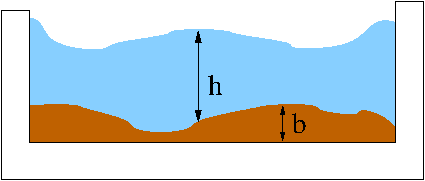
\includegraphics{basin_bathy}}
\end{DoxyImageNoCaption}
 

The shallow water equations describe the changes of water depth {\itshape h} and horizontal velocities {\itshape v$_{\mbox{x}}$ } and {\itshape v$_{\mbox{y}}$ } (in the resp. coordinate directions) over time, depending on some initial conditions -- in the case of tsunami simulation, these initial conditions could, for example, result from an initial elevation of the sea floor caused by an earthquake. The respective changes in time can be described via a system of partial differential equations\-: \[ \begin{array}{c} \displaystyle \frac{\partial h}{\partial t} + \frac{\partial (v_x h)}{\partial x} + \frac{\partial (v_y h)}{\partial y} = 0 \\[1em] \displaystyle \frac{\partial (h v_x)}{\partial t} + \frac{\partial (h v_x v_x)}{\partial x} + \frac{\partial (h v_y v_x)}{\partial y} + \frac{1}{2} g \frac{\partial (h^2)}{\partial x} = - gh \frac{\partial b}{\partial x}, \\[1em] \displaystyle \frac{\partial (h v_y)}{\partial t} + \frac{\partial (h v_x v_y)}{\partial x} + \frac{\partial (h v_y v_y)}{\partial y} + \frac{1}{2} g \frac{\partial (h^2)}{\partial y} = - gh \frac{\partial b}{\partial y}, \end{array} \] The equation for {\itshape h} is obtained, if we examine the conservation of mass in a control volume. The equations for {\itshape hv$_{\mbox{x}}$ } and {\itshape hv$_{\mbox{y}}$ } result from conservation of momentum (note that {\itshape h} is directly related to the volume, and thus the mass of the water -- thus {\itshape hv$_{\mbox{x}}$ } can be interpreted as a momentum).

The two terms involving {\itshape g} model a gravity-\/induced force ({\itshape g} being the constant for the gravitational acceleration, {\itshape g} = 9.\-81 ms$^{\mbox{-\/2}}$ ), which results from the hydrostatic pressure. The right-\/hand-\/side source terms model the effect of an uneven ocean floor ({\itshape b} obtained from respective bathymetry data).\hypertarget{index_finvol}{}\subsection{Finite Volume Discretisation}\label{index_finvol}
The shallow water equations are usually too difficult to be solved exactly -\/ hence, S\-W\-E implements simple discrete models as an approximation. As the applied numerical method (typically a Finite Volume discretization) may vary, we will stick to the basics at this point.

First, S\-W\-E assumes that the unknown functions {\itshape h(t,x,y)}, {\itshape hu(t,x,y) \-:= h(t,x,y) v$_{\mbox{x}}$ (t,x,y)}, {\itshape hv(t,x,y) \-:= h(t,x,y) v$_{\mbox{y}}$ (t,x,y)}, as well as the given sea bottom level {\itshape b(x,y)}, are approximated on a Cartesian mesh of grid cells, as illustrated below. In each grid cell, with indices {\itshape (i,j)}, the unknowns have constant values {\itshape h$_{\mbox{ij}}$ }, {\itshape hu$_{\mbox{ij}}$ }, {\itshape hv$_{\mbox{ij}}$ }, and {\itshape b$_{\mbox{ij}}$ }\-:

 
\begin{DoxyImageNoCaption}
  \mbox{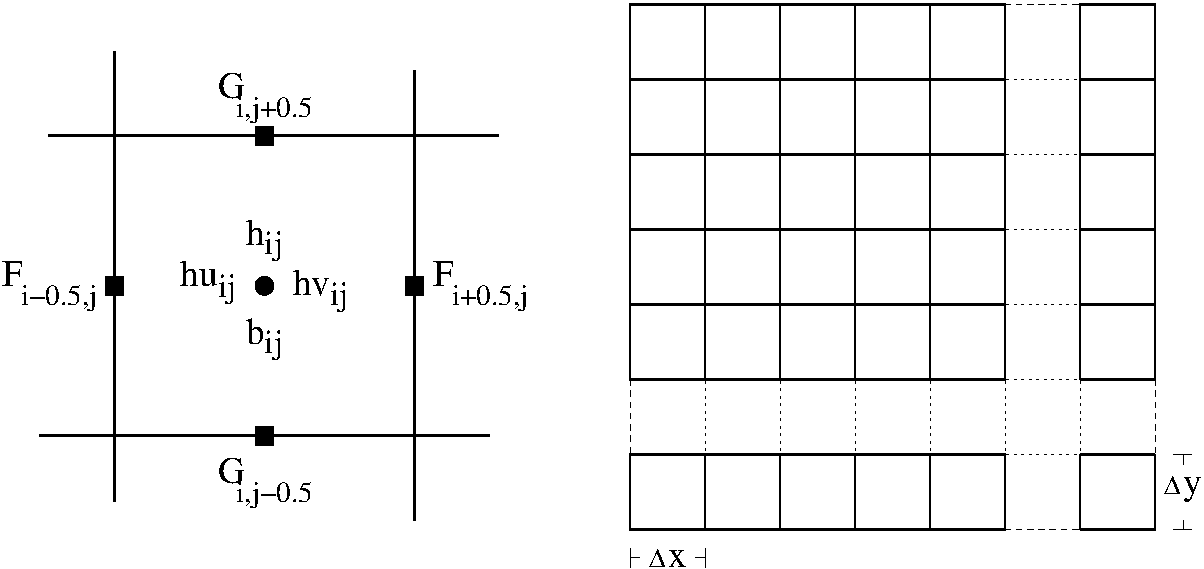
\includegraphics{grid_unknowns}}
\end{DoxyImageNoCaption}
\hypertarget{index_fluxes}{}\subsection{Computing Numerical Fluxes at Edges and Euler Time-\/\-Stepping}\label{index_fluxes}
The details of the numerical schemes are too complicated to be described in this overview. Please refer to the accompanying material. To put it short, we successively perform two main computational steps\-:
\begin{DoxyItemize}
\item we compute so-\/called {\bfseries numerical fluxes} on each edge of the grid (which approximate the transfer of mass or momentum between grid cells),
\item based on these numerical fluxes, we then update the unknowns in each cell.
\end{DoxyItemize}\hypertarget{index_impl}{}\section{Implementation and base class S\-W\-E\-\_\-\-Block}\label{index_impl}
For the simulation of the shallow water model, we thus require a regular Cartesian grid, where each grid cell carries the respective unknowns -\/ water level, momentum in x-\/ and y-\/direction, and bathymetry data. The central data structures for Cartesian grid and arrays of unknowns are provided with the abstract base class \hyperlink{classSWE__Block}{S\-W\-E\-\_\-\-Block}, which has four 2\-D arrays \hyperlink{classSWE__Block_a64a0f8f437f38b5f3b8ec5b4abdb864e}{S\-W\-E\-\_\-\-Block\-::h}, \hyperlink{classSWE__Block_aec2c1278fdb23f083216d8d397f26060}{S\-W\-E\-\_\-\-Block\-::hu}, \hyperlink{classSWE__Block_a0897aa3c2d78749f209c95e08196d831}{S\-W\-E\-\_\-\-Block\-::hv}, and \hyperlink{classSWE__Block_af7487209129f40b26ea171762754a261}{S\-W\-E\-\_\-\-Block\-::b}. To implement the behaviour of the fluid at boundaries, and also to allow the connection of several grid blocks (for parallelization or just to build more complicated computational domains), each array has an additional layer of so-\/called {\itshape ghost cells}, as illustrated in the following figure\-:


\begin{DoxyImageNoCaption}
  \mbox{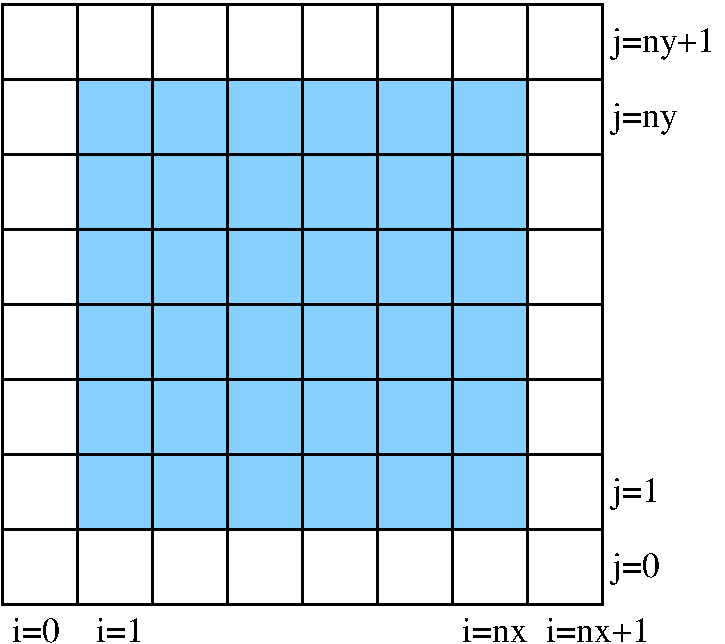
\includegraphics{ghost_cells}}
\end{DoxyImageNoCaption}
 \hypertarget{index_models}{}\subsection{Parallelisation and Different Models}\label{index_models}
In each time step, our numerical algorithm will compute the flux terms for each edge of the computational domain. To compute the fluxes, we require the values of the unknowns in both adjacent cells. At the boundaries of the fluid domain, the ghost layer makes sure that we also have two adjacent cells for the cell edges on the domain boundary. The values in the ghost layer cells will be set to values depending on the values in the adjacent fluid domain. We will model three different situations\-: \{description\} \{Outflow\-:\} \{h\}, \{u\}, and \{v\} in the ghost cell are set to the same value as in the adjacent fluid cell. This models the situation that the unknowns do not change across the domain boundary (undisturbed outflow). \{Wall\-:\} At a wall, the velocity component normal to the boundary should be \$0\$, such that no fluid can cross the boundary. To model this case, we set the normal velocity, e.\-g. \{u\mbox{[}0\mbox{]}\} at the left boundary, to the negative value of the adjacent cell\-: \{-\/u\mbox{[}1\mbox{]}\}. The interpolated value at the boundary edge will then be \$0\$ (\{h\} is identical in both cells due to the imposed boundary condition). The other two variables are set in the same way as for the outflow situation. \{Connect\-:\} With the connect case, we can connect a domain at two boundaries. If we connect the left and right boundary, we will obtain a periodically repeated domain. Here, all ghost values are determined by the values of the unknowns in the fluid cell adjacent to the connected boundary. \{description\}

To implement the boundary conditions, the class \{\hyperlink{classSWE__Block}{S\-W\-E\-\_\-\-Block}\} contains an array of four enum variables, \{boundary\mbox{[}4\mbox{]}\} (for left/right/bottom/top boundary), that can take the values {\ttfamily O\-U\-T\-F\-L\-O\-W}, {\ttfamily W\-A\-L\-L}, and {\ttfamily C\-O\-N\-N\-E\-C\-T}.\hypertarget{index_multblocks}{}\subsection{Multiple Blocks}\label{index_multblocks}
Via the connect boundary condition, it is also possible to connect several Cartesian grid blocks to build a more complicated domain. Figure fig\-:connect\} illustrates the exchange of ghost values for two connected blocks.

  
\begin{figure}
\begin{center}
  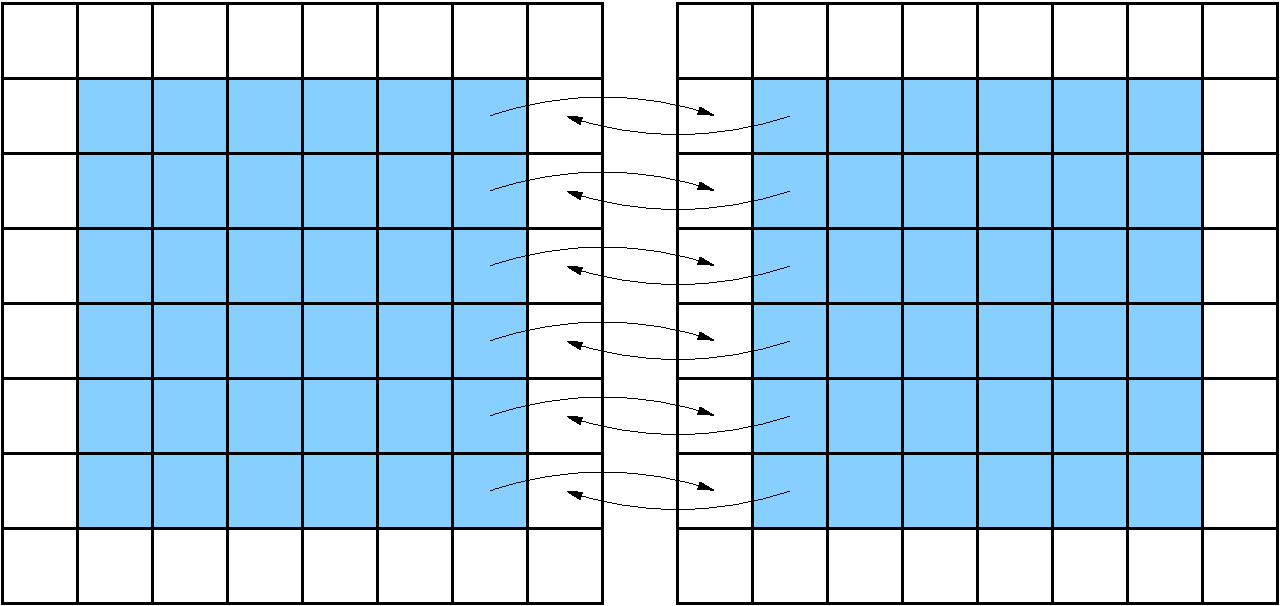
\includegraphics[width=0.8\textwidth]{pics/connect.pdf}
\end{center}
\caption{Exchange of values in ghost layers between two connected \texttt{SWE\_Block}s.}
\label{fig:connect}
\end{figure}


To store the neighbour block in case of a {\ttfamily C\-O\-N\-N\-E\-C\-T} boundary, {\ttfamily \hyperlink{classSWE__Block}{S\-W\-E\-\_\-\-Block}} contains a further array of four pointers, {\ttfamily neighbour\mbox{[}4\mbox{]}} (for left/right/bottom/top boundary), that will store a pointer to the connected adjacent {\ttfamily \hyperlink{classSWE__Block}{S\-W\-E\-\_\-\-Block}}.

The respective block approach can also be exploited for parallelisation\-: the different blocks would then be assigned to the available processors (or processor cores) -- each processor (core) works on its share of blocks, while the program has to make sure to keep the values in the ghost cells up to date (which requires explicit communication in the case of distributed-\/memory computers).\hypertarget{_}{}\subsection{}\label{_}
For each time step, our solver thus performs the following steps -- each step is implemented via a separate member function of the class \{\hyperlink{classSWE__Block}{S\-W\-E\-\_\-\-Block}\}\-: \{enumerate\}  set the values at the boundaries\-: \{set\-Boundary\-Layer()\};  compute the flux terms for all edges\-: \{compute\-Fluxes()\};  from the flux terms, compute the in/outflow balance for each cell, and compute the new values of the unknowns for the next time step\-: \{euler\-Timestep()\}. \{enumerate\}\hypertarget{_}{}\subsection{}\label{_}
The class \{\hyperlink{classSWE__Block}{S\-W\-E\-\_\-\-Block}\} contains further methods that will write the numerical solution into a sequence of files that can be read by the visualisation package Para\-View (just enter the respective folder from Para\-View -- the files will be recognised and displayed as one project). Para\-View allows to visualise the computed time-\/dependent solution (as ``movie'' or in single-\/step mode). Para\-View is pretty self-\/explanatory for our purposes, but provides an online help for further instructions.\hypertarget{_}{}\subsection{}\label{_}
We also provide a C\-U\-D\-A implementation of the simulation code (requires a computer with a C\-U\-D\-A-\/capable G\-P\-U, together with the respective drivers -- visit N\-V\-I\-D\-I\-A's website on C\-U\-D\-A for details on implementation). Apart from the fact that the simulation usually runs a lot faster on the G\-P\-U, the program is also capable of plotting the computing solution (water surface) ``on the fly''.

Finally\-: whoever thinks that they can do a better (faster, ...) implementation (visualisation, ...) of the provided code is more than welcome to do so! Feel free to contribute to S\-W\-E -\/ for questions, just contact Michael Bader (\href{mailto:bader@in.tum.de}{\tt bader@in.\-tum.\-de}). 
\chapter{Todo List}
\label{todo}
\hypertarget{todo}{}

\begin{DoxyRefList}
\item[\label{todo__todo000002}%
\hypertarget{todo__todo000002}{}%
Member \hyperlink{classio_1_1VtkWriter_aaed37669d1c38bafaf3fc36169342720}{io\-:\-:Vtk\-Writer\-:\-:Vtk\-Writer} (const std\-::string \&i\-\_\-file\-Name, const \hyperlink{classFloat2D}{Float2\-D} \&i\-\_\-b, const Boundary\-Size \&i\-\_\-boundary\-Size, int i\-\_\-n\-X, int i\-\_\-n\-Y, float i\-\_\-d\-X, float i\-\_\-d\-Y, int i\-\_\-offset\-X=0, int i\-\_\-offset\-Y=0)]This version can only handle a boundary layer of size 1 
\end{DoxyRefList}
\chapter{Deprecated List}
\label{deprecated}
\hypertarget{deprecated}{}

\begin{DoxyRefList}
\item[\label{deprecated__deprecated000001}%
\hypertarget{deprecated__deprecated000001}{}%
Member \hyperlink{help_8hh_aa10dc278c6ac60f9cd49955cbe16fbcb}{generate\-File\-Name} (std\-::string base\-Name, int time\-Step)]
\item[\label{deprecated__deprecated000003}%
\hypertarget{deprecated__deprecated000003}{}%
Member \hyperlink{help_8hh_ab05bce4e4d30d0b9fb85f81668f98f79}{generate\-File\-Name} (std\-::string base\-Name, int time\-Step, int block\-\_\-\-X, int block\-\_\-\-Y, std\-::string i\-\_\-file\-Extension=\char`\"{}.\-vts\char`\"{})]
\item[\label{deprecated__deprecated000002}%
\hypertarget{deprecated__deprecated000002}{}%
Member \hyperlink{help_8hh_a206f33ce37fa47f8635d02a1cfc9881f}{generate\-File\-Name} (std\-::string i\-\_\-base\-Name, int i\-\_\-block\-Position\-X, int i\-\_\-block\-Position\-Y, std\-::string i\-\_\-file\-Extension=\char`\"{}.\-nc\char`\"{})]
\end{DoxyRefList}
\chapter{Hierarchical Index}
\section{Class Hierarchy}
This inheritance list is sorted roughly, but not completely, alphabetically\-:\begin{DoxyCompactList}
\item \contentsline{section}{Array}{\pageref{classArray}}{}
\item \contentsline{section}{Camera}{\pageref{classCamera}}{}
\item \contentsline{section}{Controller}{\pageref{classController}}{}
\item Test\-Suite\begin{DoxyCompactList}
\item \contentsline{section}{Dimen\-Split\-Test}{\pageref{classDimenSplitTest}}{}
\end{DoxyCompactList}
\item \contentsline{section}{Float1\-D}{\pageref{classFloat1D}}{}
\item \contentsline{section}{Float2\-D}{\pageref{classFloat2D}}{}
\item \contentsline{section}{solver\-:\-:F\-Wave$<$ float $>$}{\pageref{classsolver_1_1FWave}}{}
\item \contentsline{section}{io\-:\-:Boundary\-Size}{\pageref{structio_1_1BoundarySize}}{}
\item \contentsline{section}{io\-:\-:Writer}{\pageref{classio_1_1Writer}}{}
\begin{DoxyCompactList}
\item \contentsline{section}{io\-:\-:Net\-Cdf\-Writer}{\pageref{classio_1_1NetCdfWriter}}{}
\item \contentsline{section}{io\-:\-:Vtk\-Writer}{\pageref{classio_1_1VtkWriter}}{}
\end{DoxyCompactList}
\item \contentsline{section}{Shader}{\pageref{classShader}}{}
\item \contentsline{section}{Simulation}{\pageref{classSimulation}}{}
\item \contentsline{section}{solver\-:\-:F\-Wave$<$ T $>$}{\pageref{classsolver_1_1FWave}}{}
\item \contentsline{section}{S\-W\-E\-\_\-\-Asagi\-Grid}{\pageref{classSWE__AsagiGrid}}{}
\item \contentsline{section}{S\-W\-E\-\_\-\-Block}{\pageref{classSWE__Block}}{}
\begin{DoxyCompactList}
\item \contentsline{section}{S\-W\-E\-\_\-\-Block\-C\-U\-D\-A}{\pageref{classSWE__BlockCUDA}}{}
\begin{DoxyCompactList}
\item \contentsline{section}{S\-W\-E\-\_\-\-Rusanov\-Block\-C\-U\-D\-A}{\pageref{classSWE__RusanovBlockCUDA}}{}
\item \contentsline{section}{S\-W\-E\-\_\-\-Wave\-Propagation\-Block\-Cuda}{\pageref{classSWE__WavePropagationBlockCuda}}{}
\end{DoxyCompactList}
\item \contentsline{section}{S\-W\-E\-\_\-\-Dimensional\-Splitting}{\pageref{classSWE__DimensionalSplitting}}{}
\item \contentsline{section}{S\-W\-E\-\_\-\-Rusanov\-Block}{\pageref{classSWE__RusanovBlock}}{}
\item \contentsline{section}{S\-W\-E\-\_\-\-Wave\-Accumulation\-Block}{\pageref{classSWE__WaveAccumulationBlock}}{}
\item \contentsline{section}{S\-W\-E\-\_\-\-Wave\-Propagation\-Block}{\pageref{classSWE__WavePropagationBlock}}{}
\item \contentsline{section}{S\-W\-E\-\_\-\-Wave\-Propagation\-Block\-S\-I\-M\-D}{\pageref{classSWE__WavePropagationBlockSIMD}}{}
\end{DoxyCompactList}
\item \contentsline{section}{S\-W\-E\-\_\-\-Block1\-D}{\pageref{structSWE__Block1D}}{}
\item \contentsline{section}{S\-W\-E\-\_\-\-Scenario}{\pageref{classSWE__Scenario}}{}
\begin{DoxyCompactList}
\item \contentsline{section}{S\-W\-E\-\_\-\-Artificial\-Tsunami\-Scenario}{\pageref{classSWE__ArtificialTsunamiScenario}}{}
\item \contentsline{section}{S\-W\-E\-\_\-\-Artificial\-Tsunami\-Scenario}{\pageref{classSWE__ArtificialTsunamiScenario}}{}
\item \contentsline{section}{S\-W\-E\-\_\-\-Asagi\-Scenario}{\pageref{classSWE__AsagiScenario}}{}
\item \contentsline{section}{S\-W\-E\-\_\-\-Bathymetry\-Dam\-Break\-Scenario}{\pageref{classSWE__BathymetryDamBreakScenario}}{}
\item \contentsline{section}{S\-W\-E\-\_\-\-Checkpoint\-Scenario}{\pageref{classSWE__CheckpointScenario}}{}
\item \contentsline{section}{S\-W\-E\-\_\-\-Obstacle\-Dam\-Break\-Scenario}{\pageref{classSWE__ObstacleDamBreakScenario}}{}
\item \contentsline{section}{S\-W\-E\-\_\-\-Radial\-Dam\-Break\-Scenario}{\pageref{classSWE__RadialDamBreakScenario}}{}
\item \contentsline{section}{S\-W\-E\-\_\-\-Sea\-At\-Rest\-Scenario}{\pageref{classSWE__SeaAtRestScenario}}{}
\item \contentsline{section}{S\-W\-E\-\_\-\-Seismology\-Scenario}{\pageref{classSWE__SeismologyScenario}}{}
\item \contentsline{section}{S\-W\-E\-\_\-\-Splashing\-Cone\-Scenario}{\pageref{classSWE__SplashingConeScenario}}{}
\item \contentsline{section}{S\-W\-E\-\_\-\-Splashing\-Pool\-Scenario}{\pageref{classSWE__SplashingPoolScenario}}{}
\item \contentsline{section}{S\-W\-E\-\_\-\-Tsunami\-Scenario}{\pageref{classSWE__TsunamiScenario}}{}
\end{DoxyCompactList}
\item \contentsline{section}{S\-W\-E\-\_\-\-Vis\-Info}{\pageref{classSWE__VisInfo}}{}
\begin{DoxyCompactList}
\item \contentsline{section}{S\-W\-E\-\_\-\-Asagi\-Japan\-Small\-Vis\-Info}{\pageref{classSWE__AsagiJapanSmallVisInfo}}{}
\item \contentsline{section}{S\-W\-E\-\_\-\-Bathymetry\-Dam\-Break\-Vis\-Info}{\pageref{classSWE__BathymetryDamBreakVisInfo}}{}
\end{DoxyCompactList}
\item \contentsline{section}{Text}{\pageref{classText}}{}
\item \contentsline{section}{tools\-:\-:Args}{\pageref{classtools_1_1Args}}{}
\item \contentsline{section}{tools\-:\-:Logger}{\pageref{classtools_1_1Logger}}{}
\item \contentsline{section}{tools\-:\-:Progress\-Bar}{\pageref{classtools_1_1ProgressBar}}{}
\item \contentsline{section}{V\-B\-O}{\pageref{classVBO}}{}
\item \contentsline{section}{Visualization}{\pageref{classVisualization}}{}
\end{DoxyCompactList}

\chapter{Class Index}
\section{Class List}
Here are the classes, structs, unions and interfaces with brief descriptions\-:\begin{DoxyCompactList}
\item\contentsline{section}{\hyperlink{classArray}{Array} }{\pageref{classArray}}{}
\item\contentsline{section}{\hyperlink{classCamera}{Camera} }{\pageref{classCamera}}{}
\item\contentsline{section}{\hyperlink{classController}{Controller} }{\pageref{classController}}{}
\item\contentsline{section}{\hyperlink{classDimenSplitTest}{Dimen\-Split\-Test} }{\pageref{classDimenSplitTest}}{}
\item\contentsline{section}{\hyperlink{classFloat1D}{Float1\-D} }{\pageref{classFloat1D}}{}
\item\contentsline{section}{\hyperlink{classFloat2D}{Float2\-D} }{\pageref{classFloat2D}}{}
\item\contentsline{section}{\hyperlink{structio_1_1BoundarySize}{io\-::\-Boundary\-Size} }{\pageref{structio_1_1BoundarySize}}{}
\item\contentsline{section}{\hyperlink{classio_1_1NetCdfWriter}{io\-::\-Net\-Cdf\-Writer} }{\pageref{classio_1_1NetCdfWriter}}{}
\item\contentsline{section}{\hyperlink{classio_1_1VtkWriter}{io\-::\-Vtk\-Writer} }{\pageref{classio_1_1VtkWriter}}{}
\item\contentsline{section}{\hyperlink{classio_1_1Writer}{io\-::\-Writer} }{\pageref{classio_1_1Writer}}{}
\item\contentsline{section}{\hyperlink{classShader}{Shader} }{\pageref{classShader}}{}
\item\contentsline{section}{\hyperlink{classSimulation}{Simulation} }{\pageref{classSimulation}}{}
\item\contentsline{section}{\hyperlink{classsolver_1_1FWave}{solver\-::\-F\-Wave$<$ T $>$} }{\pageref{classsolver_1_1FWave}}{}
\item\contentsline{section}{\hyperlink{classSWE__ArtificialTsunamiScenario}{S\-W\-E\-\_\-\-Artificial\-Tsunami\-Scenario} }{\pageref{classSWE__ArtificialTsunamiScenario}}{}
\item\contentsline{section}{\hyperlink{classSWE__AsagiGrid}{S\-W\-E\-\_\-\-Asagi\-Grid} }{\pageref{classSWE__AsagiGrid}}{}
\item\contentsline{section}{\hyperlink{classSWE__AsagiJapanSmallVisInfo}{S\-W\-E\-\_\-\-Asagi\-Japan\-Small\-Vis\-Info} }{\pageref{classSWE__AsagiJapanSmallVisInfo}}{}
\item\contentsline{section}{\hyperlink{classSWE__AsagiScenario}{S\-W\-E\-\_\-\-Asagi\-Scenario} }{\pageref{classSWE__AsagiScenario}}{}
\item\contentsline{section}{\hyperlink{classSWE__BathymetryDamBreakScenario}{S\-W\-E\-\_\-\-Bathymetry\-Dam\-Break\-Scenario} }{\pageref{classSWE__BathymetryDamBreakScenario}}{}
\item\contentsline{section}{\hyperlink{classSWE__BathymetryDamBreakVisInfo}{S\-W\-E\-\_\-\-Bathymetry\-Dam\-Break\-Vis\-Info} }{\pageref{classSWE__BathymetryDamBreakVisInfo}}{}
\item\contentsline{section}{\hyperlink{classSWE__Block}{S\-W\-E\-\_\-\-Block} }{\pageref{classSWE__Block}}{}
\item\contentsline{section}{\hyperlink{structSWE__Block1D}{S\-W\-E\-\_\-\-Block1\-D} }{\pageref{structSWE__Block1D}}{}
\item\contentsline{section}{\hyperlink{classSWE__BlockCUDA}{S\-W\-E\-\_\-\-Block\-C\-U\-D\-A} }{\pageref{classSWE__BlockCUDA}}{}
\item\contentsline{section}{\hyperlink{classSWE__CheckpointScenario}{S\-W\-E\-\_\-\-Checkpoint\-Scenario} }{\pageref{classSWE__CheckpointScenario}}{}
\item\contentsline{section}{\hyperlink{classSWE__DimensionalSplitting}{S\-W\-E\-\_\-\-Dimensional\-Splitting} }{\pageref{classSWE__DimensionalSplitting}}{}
\item\contentsline{section}{\hyperlink{classSWE__ObstacleDamBreakScenario}{S\-W\-E\-\_\-\-Obstacle\-Dam\-Break\-Scenario} }{\pageref{classSWE__ObstacleDamBreakScenario}}{}
\item\contentsline{section}{\hyperlink{classSWE__RadialDamBreakScenario}{S\-W\-E\-\_\-\-Radial\-Dam\-Break\-Scenario} }{\pageref{classSWE__RadialDamBreakScenario}}{}
\item\contentsline{section}{\hyperlink{classSWE__RusanovBlock}{S\-W\-E\-\_\-\-Rusanov\-Block} }{\pageref{classSWE__RusanovBlock}}{}
\item\contentsline{section}{\hyperlink{classSWE__RusanovBlockCUDA}{S\-W\-E\-\_\-\-Rusanov\-Block\-C\-U\-D\-A} }{\pageref{classSWE__RusanovBlockCUDA}}{}
\item\contentsline{section}{\hyperlink{classSWE__Scenario}{S\-W\-E\-\_\-\-Scenario} }{\pageref{classSWE__Scenario}}{}
\item\contentsline{section}{\hyperlink{classSWE__SeaAtRestScenario}{S\-W\-E\-\_\-\-Sea\-At\-Rest\-Scenario} }{\pageref{classSWE__SeaAtRestScenario}}{}
\item\contentsline{section}{\hyperlink{classSWE__SeismologyScenario}{S\-W\-E\-\_\-\-Seismology\-Scenario} }{\pageref{classSWE__SeismologyScenario}}{}
\item\contentsline{section}{\hyperlink{classSWE__SplashingConeScenario}{S\-W\-E\-\_\-\-Splashing\-Cone\-Scenario} }{\pageref{classSWE__SplashingConeScenario}}{}
\item\contentsline{section}{\hyperlink{classSWE__SplashingPoolScenario}{S\-W\-E\-\_\-\-Splashing\-Pool\-Scenario} }{\pageref{classSWE__SplashingPoolScenario}}{}
\item\contentsline{section}{\hyperlink{classSWE__TsunamiScenario}{S\-W\-E\-\_\-\-Tsunami\-Scenario} }{\pageref{classSWE__TsunamiScenario}}{}
\item\contentsline{section}{\hyperlink{classSWE__VisInfo}{S\-W\-E\-\_\-\-Vis\-Info} }{\pageref{classSWE__VisInfo}}{}
\item\contentsline{section}{\hyperlink{classSWE__WaveAccumulationBlock}{S\-W\-E\-\_\-\-Wave\-Accumulation\-Block} }{\pageref{classSWE__WaveAccumulationBlock}}{}
\item\contentsline{section}{\hyperlink{classSWE__WavePropagationBlock}{S\-W\-E\-\_\-\-Wave\-Propagation\-Block} }{\pageref{classSWE__WavePropagationBlock}}{}
\item\contentsline{section}{\hyperlink{classSWE__WavePropagationBlockCuda}{S\-W\-E\-\_\-\-Wave\-Propagation\-Block\-Cuda} }{\pageref{classSWE__WavePropagationBlockCuda}}{}
\item\contentsline{section}{\hyperlink{classSWE__WavePropagationBlockSIMD}{S\-W\-E\-\_\-\-Wave\-Propagation\-Block\-S\-I\-M\-D} }{\pageref{classSWE__WavePropagationBlockSIMD}}{}
\item\contentsline{section}{\hyperlink{classText}{Text} }{\pageref{classText}}{}
\item\contentsline{section}{\hyperlink{classtools_1_1Args}{tools\-::\-Args} }{\pageref{classtools_1_1Args}}{}
\item\contentsline{section}{\hyperlink{classtools_1_1Logger}{tools\-::\-Logger} }{\pageref{classtools_1_1Logger}}{}
\item\contentsline{section}{\hyperlink{classtools_1_1ProgressBar}{tools\-::\-Progress\-Bar} }{\pageref{classtools_1_1ProgressBar}}{}
\item\contentsline{section}{\hyperlink{classVBO}{V\-B\-O} }{\pageref{classVBO}}{}
\item\contentsline{section}{\hyperlink{classVisualization}{Visualization} }{\pageref{classVisualization}}{}
\end{DoxyCompactList}

\chapter{File Index}
\section{File List}
Here is a list of all documented files with brief descriptions\-:\begin{DoxyCompactList}
\item\contentsline{section}{/home/sascha/\-Dokumente/\-Projects/\-Tsun\-Sim/\-S\-W\-E/src/blocks/\hyperlink{SWE__Block_8cpp}{S\-W\-E\-\_\-\-Block.\-cpp} }{\pageref{SWE__Block_8cpp}}{}
\item\contentsline{section}{/home/sascha/\-Dokumente/\-Projects/\-Tsun\-Sim/\-S\-W\-E/src/blocks/\hyperlink{SWE__Block_8hh}{S\-W\-E\-\_\-\-Block.\-hh} }{\pageref{SWE__Block_8hh}}{}
\item\contentsline{section}{/home/sascha/\-Dokumente/\-Projects/\-Tsun\-Sim/\-S\-W\-E/src/blocks/\hyperlink{SWE__DimensionalSplitting_8hpp}{S\-W\-E\-\_\-\-Dimensional\-Splitting.\-hpp} }{\pageref{SWE__DimensionalSplitting_8hpp}}{}
\item\contentsline{section}{/home/sascha/\-Dokumente/\-Projects/\-Tsun\-Sim/\-S\-W\-E/src/blocks/\hyperlink{SWE__WaveAccumulationBlock_8cpp}{S\-W\-E\-\_\-\-Wave\-Accumulation\-Block.\-cpp} }{\pageref{SWE__WaveAccumulationBlock_8cpp}}{}
\item\contentsline{section}{/home/sascha/\-Dokumente/\-Projects/\-Tsun\-Sim/\-S\-W\-E/src/blocks/\hyperlink{SWE__WaveAccumulationBlock_8hh}{S\-W\-E\-\_\-\-Wave\-Accumulation\-Block.\-hh} }{\pageref{SWE__WaveAccumulationBlock_8hh}}{}
\item\contentsline{section}{/home/sascha/\-Dokumente/\-Projects/\-Tsun\-Sim/\-S\-W\-E/src/blocks/\hyperlink{SWE__WavePropagationBlock_8cpp}{S\-W\-E\-\_\-\-Wave\-Propagation\-Block.\-cpp} }{\pageref{SWE__WavePropagationBlock_8cpp}}{}
\item\contentsline{section}{/home/sascha/\-Dokumente/\-Projects/\-Tsun\-Sim/\-S\-W\-E/src/blocks/\hyperlink{SWE__WavePropagationBlock_8hh}{S\-W\-E\-\_\-\-Wave\-Propagation\-Block.\-hh} }{\pageref{SWE__WavePropagationBlock_8hh}}{}
\item\contentsline{section}{/home/sascha/\-Dokumente/\-Projects/\-Tsun\-Sim/\-S\-W\-E/src/blocks/\hyperlink{SWE__WavePropagationBlockSIMD_8cpp}{S\-W\-E\-\_\-\-Wave\-Propagation\-Block\-S\-I\-M\-D.\-cpp} }{\pageref{SWE__WavePropagationBlockSIMD_8cpp}}{}
\item\contentsline{section}{/home/sascha/\-Dokumente/\-Projects/\-Tsun\-Sim/\-S\-W\-E/src/blocks/\hyperlink{SWE__WavePropagationBlockSIMD_8hh}{S\-W\-E\-\_\-\-Wave\-Propagation\-Block\-S\-I\-M\-D.\-hh} }{\pageref{SWE__WavePropagationBlockSIMD_8hh}}{}
\item\contentsline{section}{/home/sascha/\-Dokumente/\-Projects/\-Tsun\-Sim/\-S\-W\-E/src/blocks/cuda/\hyperlink{SWE__BlockCUDA_8cu}{S\-W\-E\-\_\-\-Block\-C\-U\-D\-A.\-cu} }{\pageref{SWE__BlockCUDA_8cu}}{}
\item\contentsline{section}{/home/sascha/\-Dokumente/\-Projects/\-Tsun\-Sim/\-S\-W\-E/src/blocks/cuda/\hyperlink{SWE__BlockCUDA_8hh}{S\-W\-E\-\_\-\-Block\-C\-U\-D\-A.\-hh} }{\pageref{SWE__BlockCUDA_8hh}}{}
\item\contentsline{section}{/home/sascha/\-Dokumente/\-Projects/\-Tsun\-Sim/\-S\-W\-E/src/blocks/cuda/\hyperlink{SWE__BlockCUDA__kernels_8cu}{S\-W\-E\-\_\-\-Block\-C\-U\-D\-A\-\_\-kernels.\-cu} }{\pageref{SWE__BlockCUDA__kernels_8cu}}{}
\item\contentsline{section}{/home/sascha/\-Dokumente/\-Projects/\-Tsun\-Sim/\-S\-W\-E/src/blocks/cuda/\hyperlink{SWE__BlockCUDA__kernels_8hh}{S\-W\-E\-\_\-\-Block\-C\-U\-D\-A\-\_\-kernels.\-hh} }{\pageref{SWE__BlockCUDA__kernels_8hh}}{}
\item\contentsline{section}{/home/sascha/\-Dokumente/\-Projects/\-Tsun\-Sim/\-S\-W\-E/src/blocks/cuda/\hyperlink{SWE__WavePropagationBlockCuda_8cu}{S\-W\-E\-\_\-\-Wave\-Propagation\-Block\-Cuda.\-cu} }{\pageref{SWE__WavePropagationBlockCuda_8cu}}{}
\item\contentsline{section}{/home/sascha/\-Dokumente/\-Projects/\-Tsun\-Sim/\-S\-W\-E/src/blocks/cuda/\hyperlink{SWE__WavePropagationBlockCuda_8hh}{S\-W\-E\-\_\-\-Wave\-Propagation\-Block\-Cuda.\-hh} }{\pageref{SWE__WavePropagationBlockCuda_8hh}}{}
\item\contentsline{section}{/home/sascha/\-Dokumente/\-Projects/\-Tsun\-Sim/\-S\-W\-E/src/blocks/cuda/\hyperlink{SWE__WavePropagationBlockCuda__kernels_8cu}{S\-W\-E\-\_\-\-Wave\-Propagation\-Block\-Cuda\-\_\-kernels.\-cu} }{\pageref{SWE__WavePropagationBlockCuda__kernels_8cu}}{}
\item\contentsline{section}{/home/sascha/\-Dokumente/\-Projects/\-Tsun\-Sim/\-S\-W\-E/src/blocks/cuda/\hyperlink{SWE__WavePropagationBlockCuda__kernels_8hh}{S\-W\-E\-\_\-\-Wave\-Propagation\-Block\-Cuda\-\_\-kernels.\-hh} }{\pageref{SWE__WavePropagationBlockCuda__kernels_8hh}}{}
\item\contentsline{section}{/home/sascha/\-Dokumente/\-Projects/\-Tsun\-Sim/\-S\-W\-E/src/blocks/rusanov/\hyperlink{SWE__RusanovBlock_8cpp}{S\-W\-E\-\_\-\-Rusanov\-Block.\-cpp} }{\pageref{SWE__RusanovBlock_8cpp}}{}
\item\contentsline{section}{/home/sascha/\-Dokumente/\-Projects/\-Tsun\-Sim/\-S\-W\-E/src/blocks/rusanov/\hyperlink{SWE__RusanovBlock_8hh}{S\-W\-E\-\_\-\-Rusanov\-Block.\-hh} }{\pageref{SWE__RusanovBlock_8hh}}{}
\item\contentsline{section}{/home/sascha/\-Dokumente/\-Projects/\-Tsun\-Sim/\-S\-W\-E/src/blocks/rusanov/\hyperlink{SWE__RusanovBlockCUDA_8cu}{S\-W\-E\-\_\-\-Rusanov\-Block\-C\-U\-D\-A.\-cu} }{\pageref{SWE__RusanovBlockCUDA_8cu}}{}
\item\contentsline{section}{/home/sascha/\-Dokumente/\-Projects/\-Tsun\-Sim/\-S\-W\-E/src/blocks/rusanov/\hyperlink{SWE__RusanovBlockCUDA_8hh}{S\-W\-E\-\_\-\-Rusanov\-Block\-C\-U\-D\-A.\-hh} }{\pageref{SWE__RusanovBlockCUDA_8hh}}{}
\item\contentsline{section}{/home/sascha/\-Dokumente/\-Projects/\-Tsun\-Sim/\-S\-W\-E/src/blocks/rusanov/\hyperlink{SWE__RusanovBlockCUDA__kernels_8cu}{S\-W\-E\-\_\-\-Rusanov\-Block\-C\-U\-D\-A\-\_\-kernels.\-cu} }{\pageref{SWE__RusanovBlockCUDA__kernels_8cu}}{}
\item\contentsline{section}{/home/sascha/\-Dokumente/\-Projects/\-Tsun\-Sim/\-S\-W\-E/src/blocks/rusanov/\hyperlink{SWE__RusanovBlockCUDA__kernels_8hh}{S\-W\-E\-\_\-\-Rusanov\-Block\-C\-U\-D\-A\-\_\-kernels.\-hh} }{\pageref{SWE__RusanovBlockCUDA__kernels_8hh}}{}
\item\contentsline{section}{/home/sascha/\-Dokumente/\-Projects/\-Tsun\-Sim/\-S\-W\-E/src/examples/\hyperlink{swe__mpi_8cpp}{swe\-\_\-mpi.\-cpp} }{\pageref{swe__mpi_8cpp}}{}
\item\contentsline{section}{/home/sascha/\-Dokumente/\-Projects/\-Tsun\-Sim/\-S\-W\-E/src/examples/\hyperlink{swe__simple_8cpp}{swe\-\_\-simple.\-cpp} }{\pageref{swe__simple_8cpp}}{}
\item\contentsline{section}{/home/sascha/\-Dokumente/\-Projects/\-Tsun\-Sim/\-S\-W\-E/src/opengl/{\bfseries camera.\-h} }{\pageref{camera_8h}}{}
\item\contentsline{section}{/home/sascha/\-Dokumente/\-Projects/\-Tsun\-Sim/\-S\-W\-E/src/opengl/{\bfseries controller.\-h} }{\pageref{controller_8h}}{}
\item\contentsline{section}{/home/sascha/\-Dokumente/\-Projects/\-Tsun\-Sim/\-S\-W\-E/src/opengl/{\bfseries shader.\-h} }{\pageref{shader_8h}}{}
\item\contentsline{section}{/home/sascha/\-Dokumente/\-Projects/\-Tsun\-Sim/\-S\-W\-E/src/opengl/{\bfseries simulation.\-h} }{\pageref{simulation_8h}}{}
\item\contentsline{section}{/home/sascha/\-Dokumente/\-Projects/\-Tsun\-Sim/\-S\-W\-E/src/opengl/{\bfseries text.\-h} }{\pageref{text_8h}}{}
\item\contentsline{section}{/home/sascha/\-Dokumente/\-Projects/\-Tsun\-Sim/\-S\-W\-E/src/opengl/\hyperlink{vbo_8cpp}{vbo.\-cpp} }{\pageref{vbo_8cpp}}{}
\item\contentsline{section}{/home/sascha/\-Dokumente/\-Projects/\-Tsun\-Sim/\-S\-W\-E/src/opengl/\hyperlink{vbo_8h}{vbo.\-h} }{\pageref{vbo_8h}}{}
\item\contentsline{section}{/home/sascha/\-Dokumente/\-Projects/\-Tsun\-Sim/\-S\-W\-E/src/opengl/{\bfseries visualization.\-h} }{\pageref{visualization_8h}}{}
\item\contentsline{section}{/home/sascha/\-Dokumente/\-Projects/\-Tsun\-Sim/\-S\-W\-E/src/scenarios/\hyperlink{SWE__AsagiScenario_8cpp}{S\-W\-E\-\_\-\-Asagi\-Scenario.\-cpp} }{\pageref{SWE__AsagiScenario_8cpp}}{}
\item\contentsline{section}{/home/sascha/\-Dokumente/\-Projects/\-Tsun\-Sim/\-S\-W\-E/src/scenarios/\hyperlink{SWE__AsagiScenario_8hh}{S\-W\-E\-\_\-\-Asagi\-Scenario.\-hh} }{\pageref{SWE__AsagiScenario_8hh}}{}
\item\contentsline{section}{/home/sascha/\-Dokumente/\-Projects/\-Tsun\-Sim/\-S\-W\-E/src/scenarios/\hyperlink{SWE__AsagiScenario__vis_8hh}{S\-W\-E\-\_\-\-Asagi\-Scenario\-\_\-vis.\-hh} }{\pageref{SWE__AsagiScenario__vis_8hh}}{}
\item\contentsline{section}{/home/sascha/\-Dokumente/\-Projects/\-Tsun\-Sim/\-S\-W\-E/src/scenarios/\hyperlink{SWE__Scenario_8hh}{S\-W\-E\-\_\-\-Scenario.\-hh} }{\pageref{SWE__Scenario_8hh}}{}
\item\contentsline{section}{/home/sascha/\-Dokumente/\-Projects/\-Tsun\-Sim/\-S\-W\-E/src/scenarios/\hyperlink{SWE__simple__scenarios_8hh}{S\-W\-E\-\_\-simple\-\_\-scenarios.\-hh} }{\pageref{SWE__simple__scenarios_8hh}}{}
\item\contentsline{section}{/home/sascha/\-Dokumente/\-Projects/\-Tsun\-Sim/\-S\-W\-E/src/scenarios/{\bfseries S\-W\-E\-\_\-simple\-\_\-scenarios\-\_\-vis.\-hh} }{\pageref{SWE__simple__scenarios__vis_8hh}}{}
\item\contentsline{section}{/home/sascha/\-Dokumente/\-Projects/\-Tsun\-Sim/\-S\-W\-E/src/scenarios/\hyperlink{SWE__VisInfo_8hh}{S\-W\-E\-\_\-\-Vis\-Info.\-hh} }{\pageref{SWE__VisInfo_8hh}}{}
\item\contentsline{section}{/home/sascha/\-Dokumente/\-Projects/\-Tsun\-Sim/\-S\-W\-E/src/tools/\hyperlink{args_8hh}{args.\-hh} }{\pageref{args_8hh}}{}
\item\contentsline{section}{/home/sascha/\-Dokumente/\-Projects/\-Tsun\-Sim/\-S\-W\-E/src/tools/\hyperlink{help_8hh}{help.\-hh} }{\pageref{help_8hh}}{}
\item\contentsline{section}{/home/sascha/\-Dokumente/\-Projects/\-Tsun\-Sim/\-S\-W\-E/src/tools/\hyperlink{Logger_8cpp}{Logger.\-cpp} }{\pageref{Logger_8cpp}}{}
\item\contentsline{section}{/home/sascha/\-Dokumente/\-Projects/\-Tsun\-Sim/\-S\-W\-E/src/tools/\hyperlink{Logger_8hh}{Logger.\-hh} }{\pageref{Logger_8hh}}{}
\item\contentsline{section}{/home/sascha/\-Dokumente/\-Projects/\-Tsun\-Sim/\-S\-W\-E/src/tools/\hyperlink{ProgressBar_8hh}{Progress\-Bar.\-hh} }{\pageref{ProgressBar_8hh}}{}
\item\contentsline{section}{/home/sascha/\-Dokumente/\-Projects/\-Tsun\-Sim/\-S\-W\-E/src/writer/\hyperlink{NetCdfWriter_8cpp}{Net\-Cdf\-Writer.\-cpp} }{\pageref{NetCdfWriter_8cpp}}{}
\item\contentsline{section}{/home/sascha/\-Dokumente/\-Projects/\-Tsun\-Sim/\-S\-W\-E/src/writer/\hyperlink{NetCdfWriter_8hh}{Net\-Cdf\-Writer.\-hh} }{\pageref{NetCdfWriter_8hh}}{}
\item\contentsline{section}{/home/sascha/\-Dokumente/\-Projects/\-Tsun\-Sim/\-S\-W\-E/src/writer/\hyperlink{VtkWriter_8cpp}{Vtk\-Writer.\-cpp} }{\pageref{VtkWriter_8cpp}}{}
\item\contentsline{section}{/home/sascha/\-Dokumente/\-Projects/\-Tsun\-Sim/\-S\-W\-E/src/writer/\hyperlink{VtkWriter_8hh}{Vtk\-Writer.\-hh} }{\pageref{VtkWriter_8hh}}{}
\item\contentsline{section}{/home/sascha/\-Dokumente/\-Projects/\-Tsun\-Sim/\-S\-W\-E/src/writer/\hyperlink{Writer_8hh}{Writer.\-hh} }{\pageref{Writer_8hh}}{}
\item\contentsline{section}{/home/sascha/\-Dokumente/\-Projects/\-Tsun\-Sim/\-S\-W\-E/submodules/swe\-\_\-solvers/{\bfseries F\-Wave.\-hpp} }{\pageref{FWave_8hpp}}{}
\end{DoxyCompactList}

\chapter{Class Documentation}
\hypertarget{classCamera}{\section{Camera Class Reference}
\label{classCamera}\index{Camera@{Camera}}
}
\subsection*{Public Member Functions}
\begin{DoxyCompactItemize}
\item 
\hyperlink{classCamera_abd689594d0f4923a86c6246eb6f0b19b}{Camera} (const char $\ast$window\-\_\-title)
\item 
void \hyperlink{classCamera_a778673e0a23face89f7bcc091d6cde90}{set\-Camera} ()
\item 
\hypertarget{classCamera_a02be8aa0dbef77e02dddc715a726fb67}{void {\bfseries reset} ()}\label{classCamera_a02be8aa0dbef77e02dddc715a726fb67}

\item 
void \hyperlink{classCamera_a0d7176e717c810846265bcdcd9b84dfc}{view\-Distance} (float view\-Distance)
\item 
void \hyperlink{classCamera_a33f913cbf4a80da781dba52394874510}{orient} (float ang\-X, float ang\-Y)
\item 
void \hyperlink{classCamera_a8c2cbaf57e3af080a081526971b444d5}{zoom\-In} (float scale\-Factor)
\item 
void \hyperlink{classCamera_aab00e9276abe4e02232496de6a7853da}{zoom\-Out} (float scale\-Factor)
\item 
void \hyperlink{classCamera_a3c26259ca3463566848fc69e4c7fe286}{start\-Panning} (int x\-Pos, int y\-Pos)
\item 
void \hyperlink{classCamera_abf9c2431830d130ccde9a942e203acb3}{panning} (int new\-X, int new\-Y)
\item 
void \hyperlink{classCamera_addc91448d3f388b8410dc9cf98b571e8}{display\-Image} ()
\end{DoxyCompactItemize}


\subsection{Constructor \& Destructor Documentation}
\hypertarget{classCamera_abd689594d0f4923a86c6246eb6f0b19b}{\index{Camera@{Camera}!Camera@{Camera}}
\index{Camera@{Camera}!Camera@{Camera}}
\subsubsection[{Camera}]{\setlength{\rightskip}{0pt plus 5cm}Camera\-::\-Camera (
\begin{DoxyParamCaption}
\item[{const char $\ast$}]{window\-\_\-title}
\end{DoxyParamCaption}
)}}\label{classCamera_abd689594d0f4923a86c6246eb6f0b19b}
Constructor \begin{DoxyVerb}@param view_distance        initial view distance from the origin 
@param window_title         title of the current window\end{DoxyVerb}
 

\subsection{Member Function Documentation}
\hypertarget{classCamera_addc91448d3f388b8410dc9cf98b571e8}{\index{Camera@{Camera}!display\-Image@{display\-Image}}
\index{display\-Image@{display\-Image}!Camera@{Camera}}
\subsubsection[{display\-Image}]{\setlength{\rightskip}{0pt plus 5cm}void Camera\-::display\-Image (
\begin{DoxyParamCaption}
{}
\end{DoxyParamCaption}
)}}\label{classCamera_addc91448d3f388b8410dc9cf98b571e8}
Calculates the current framerate, updates the window title and swaps framebuffers to display the new image \hypertarget{classCamera_a33f913cbf4a80da781dba52394874510}{\index{Camera@{Camera}!orient@{orient}}
\index{orient@{orient}!Camera@{Camera}}
\subsubsection[{orient}]{\setlength{\rightskip}{0pt plus 5cm}void Camera\-::orient (
\begin{DoxyParamCaption}
\item[{float}]{angle\-\_\-d\-X, }
\item[{float}]{angle\-\_\-d\-Y}
\end{DoxyParamCaption}
)}}\label{classCamera_a33f913cbf4a80da781dba52394874510}
Increment viewing orientation of the camera \begin{DoxyVerb}@param angle_dX             angle relative to the x-axis
@param angle_dY             angle relative to the rotated y-axis\end{DoxyVerb}
 \hypertarget{classCamera_abf9c2431830d130ccde9a942e203acb3}{\index{Camera@{Camera}!panning@{panning}}
\index{panning@{panning}!Camera@{Camera}}
\subsubsection[{panning}]{\setlength{\rightskip}{0pt plus 5cm}void Camera\-::panning (
\begin{DoxyParamCaption}
\item[{int}]{new\-X, }
\item[{int}]{new\-Y}
\end{DoxyParamCaption}
)}}\label{classCamera_abf9c2431830d130ccde9a942e203acb3}
User drags our object. Transform screen coordinates into world coordinates and update the objects position \hypertarget{classCamera_a778673e0a23face89f7bcc091d6cde90}{\index{Camera@{Camera}!set\-Camera@{set\-Camera}}
\index{set\-Camera@{set\-Camera}!Camera@{Camera}}
\subsubsection[{set\-Camera}]{\setlength{\rightskip}{0pt plus 5cm}void Camera\-::set\-Camera (
\begin{DoxyParamCaption}
{}
\end{DoxyParamCaption}
)}}\label{classCamera_a778673e0a23face89f7bcc091d6cde90}
Set the camera via glu\-Look\-At and set the light position afterwards \hypertarget{classCamera_a3c26259ca3463566848fc69e4c7fe286}{\index{Camera@{Camera}!start\-Panning@{start\-Panning}}
\index{start\-Panning@{start\-Panning}!Camera@{Camera}}
\subsubsection[{start\-Panning}]{\setlength{\rightskip}{0pt plus 5cm}void Camera\-::start\-Panning (
\begin{DoxyParamCaption}
\item[{int}]{x\-Pos, }
\item[{int}]{y\-Pos}
\end{DoxyParamCaption}
)}}\label{classCamera_a3c26259ca3463566848fc69e4c7fe286}
User starts dragging. Remember the old mouse coordinates. \hypertarget{classCamera_a0d7176e717c810846265bcdcd9b84dfc}{\index{Camera@{Camera}!view\-Distance@{view\-Distance}}
\index{view\-Distance@{view\-Distance}!Camera@{Camera}}
\subsubsection[{view\-Distance}]{\setlength{\rightskip}{0pt plus 5cm}void Camera\-::view\-Distance (
\begin{DoxyParamCaption}
\item[{float}]{view\-Distance}
\end{DoxyParamCaption}
)}}\label{classCamera_a0d7176e717c810846265bcdcd9b84dfc}
Set the view distance \hypertarget{classCamera_a8c2cbaf57e3af080a081526971b444d5}{\index{Camera@{Camera}!zoom\-In@{zoom\-In}}
\index{zoom\-In@{zoom\-In}!Camera@{Camera}}
\subsubsection[{zoom\-In}]{\setlength{\rightskip}{0pt plus 5cm}void Camera\-::zoom\-In (
\begin{DoxyParamCaption}
\item[{float}]{scale\-Factor}
\end{DoxyParamCaption}
)}}\label{classCamera_a8c2cbaf57e3af080a081526971b444d5}
Zoom in \begin{DoxyVerb}@param scaleFactor          factor which is used for zooming                        \end{DoxyVerb}
 \hypertarget{classCamera_aab00e9276abe4e02232496de6a7853da}{\index{Camera@{Camera}!zoom\-Out@{zoom\-Out}}
\index{zoom\-Out@{zoom\-Out}!Camera@{Camera}}
\subsubsection[{zoom\-Out}]{\setlength{\rightskip}{0pt plus 5cm}void Camera\-::zoom\-Out (
\begin{DoxyParamCaption}
\item[{float}]{scale\-Factor}
\end{DoxyParamCaption}
)}}\label{classCamera_aab00e9276abe4e02232496de6a7853da}
Zoom out \begin{DoxyVerb}@param scaleFactor          factor which is used for zooming                        \end{DoxyVerb}
 

The documentation for this class was generated from the following files\-:\begin{DoxyCompactItemize}
\item 
src/opengl/camera.\-h\item 
src/opengl/camera.\-cpp\end{DoxyCompactItemize}

\hypertarget{classController}{\section{Controller Class Reference}
\label{classController}\index{Controller@{Controller}}
}
\subsection*{Public Member Functions}
\begin{DoxyCompactItemize}
\item 
\hyperlink{classController_a2b55acad847052f83457ad6d309befd6}{Controller} (\hyperlink{classSimulation}{Simulation} $\ast$sim, \hyperlink{classVisualization}{Visualization} $\ast$vis)
\item 
bool \hyperlink{classController_abaacee3e0b0630e6c664145e88fefefb}{handle\-Events} ()
\item 
bool \hyperlink{classController_a93e6b148bdad66a036f0a5798491c29b}{has\-Focus} ()
\item 
bool \hyperlink{classController_af4a1555d7e04ef235749b81302bbd092}{is\-Paused} ()
\end{DoxyCompactItemize}


\subsection{Constructor \& Destructor Documentation}
\hypertarget{classController_a2b55acad847052f83457ad6d309befd6}{\index{Controller@{Controller}!Controller@{Controller}}
\index{Controller@{Controller}!Controller@{Controller}}
\subsubsection[{Controller}]{\setlength{\rightskip}{0pt plus 5cm}Controller\-::\-Controller (
\begin{DoxyParamCaption}
\item[{{\bf Simulation} $\ast$}]{sim, }
\item[{{\bf Visualization} $\ast$}]{vis}
\end{DoxyParamCaption}
)}}\label{classController_a2b55acad847052f83457ad6d309befd6}
Constructor \begin{DoxyVerb}@param sim                          instance of simulation class
@param vis                          instance of visualization class\end{DoxyVerb}
 

\subsection{Member Function Documentation}
\hypertarget{classController_abaacee3e0b0630e6c664145e88fefefb}{\index{Controller@{Controller}!handle\-Events@{handle\-Events}}
\index{handle\-Events@{handle\-Events}!Controller@{Controller}}
\subsubsection[{handle\-Events}]{\setlength{\rightskip}{0pt plus 5cm}bool Controller\-::handle\-Events (
\begin{DoxyParamCaption}
{}
\end{DoxyParamCaption}
)}}\label{classController_abaacee3e0b0630e6c664145e88fefefb}
Process all user events in a loop Returns true, when user wants to quit \hypertarget{classController_a93e6b148bdad66a036f0a5798491c29b}{\index{Controller@{Controller}!has\-Focus@{has\-Focus}}
\index{has\-Focus@{has\-Focus}!Controller@{Controller}}
\subsubsection[{has\-Focus}]{\setlength{\rightskip}{0pt plus 5cm}bool Controller\-::has\-Focus (
\begin{DoxyParamCaption}
{}
\end{DoxyParamCaption}
)}}\label{classController_a93e6b148bdad66a036f0a5798491c29b}
Returns true, when window has focus \hypertarget{classController_af4a1555d7e04ef235749b81302bbd092}{\index{Controller@{Controller}!is\-Paused@{is\-Paused}}
\index{is\-Paused@{is\-Paused}!Controller@{Controller}}
\subsubsection[{is\-Paused}]{\setlength{\rightskip}{0pt plus 5cm}bool Controller\-::is\-Paused (
\begin{DoxyParamCaption}
{}
\end{DoxyParamCaption}
)}}\label{classController_af4a1555d7e04ef235749b81302bbd092}
Return whether program is currently paused 

The documentation for this class was generated from the following files\-:\begin{DoxyCompactItemize}
\item 
src/opengl/controller.\-h\item 
src/opengl/controller.\-cpp\end{DoxyCompactItemize}

\hypertarget{classFloat1D}{\section{Float1\-D Class Reference}
\label{classFloat1D}\index{Float1\-D@{Float1\-D}}
}


{\ttfamily \#include $<$help.\-hh$>$}

\subsection*{Public Member Functions}
\begin{DoxyCompactItemize}
\item 
\hypertarget{classFloat1D_abac72fb922ec7c6d05818be856ede9a2}{{\bfseries Float1\-D} (float $\ast$\-\_\-elem, int \-\_\-rows, int \-\_\-stride=1)}\label{classFloat1D_abac72fb922ec7c6d05818be856ede9a2}

\item 
\hypertarget{classFloat1D_ab5c51078ce867170570f54f6fed7af7e}{std\-::string {\bfseries To\-String} ()}\label{classFloat1D_ab5c51078ce867170570f54f6fed7af7e}

\item 
\hypertarget{classFloat1D_a4602b1598eaf2e130a55df93b9723e91}{float \& {\bfseries operator\mbox{[}$\,$\mbox{]}} (int i)}\label{classFloat1D_a4602b1598eaf2e130a55df93b9723e91}

\item 
\hypertarget{classFloat1D_af3356b364d5ff56f3740729724da0467}{const float \& {\bfseries operator\mbox{[}$\,$\mbox{]}} (int i) const }\label{classFloat1D_af3356b364d5ff56f3740729724da0467}

\item 
\hypertarget{classFloat1D_a2e7889e514588f539a8dc47c75e70601}{float $\ast$ {\bfseries elem\-Vector} ()}\label{classFloat1D_a2e7889e514588f539a8dc47c75e70601}

\item 
\hypertarget{classFloat1D_a8af61aafa38fdab2e9bdbeb7eba563c6}{void {\bfseries force\-Size} (int new\-Size)}\label{classFloat1D_a8af61aafa38fdab2e9bdbeb7eba563c6}

\item 
\hypertarget{classFloat1D_a247a2e783f7300467c55fa2e7b19aa43}{int {\bfseries get\-Size} () const }\label{classFloat1D_a247a2e783f7300467c55fa2e7b19aa43}

\end{DoxyCompactItemize}


\subsection{Detailed Description}
class \hyperlink{classFloat1D}{Float1\-D} is a proxy class that can represent, for example, a column or row vector of a \hyperlink{classFloat2D}{Float2\-D} array, where row (sub-\/)arrays are stored with a respective stride. Besides constructor/deconstructor, the class provides overloading of the \mbox{[}\mbox{]}-\/operator, such that elements can be accessed as v\mbox{[}i\mbox{]} (independent of the stride). The class will never allocate separate memory for the vectors, but point to the interior data structure of \hyperlink{classFloat2D}{Float2\-D} (or other \char`\"{}host\char`\"{} data structures). 

The documentation for this class was generated from the following file\-:\begin{DoxyCompactItemize}
\item 
src/tools/\hyperlink{help_8hh}{help.\-hh}\end{DoxyCompactItemize}

\hypertarget{classFloat2D}{\section{Float2\-D Class Reference}
\label{classFloat2D}\index{Float2\-D@{Float2\-D}}
}


{\ttfamily \#include $<$help.\-hh$>$}

\subsection*{Public Member Functions}
\begin{DoxyCompactItemize}
\item 
\hyperlink{classFloat2D_aceac75782e5db5cb644a893de73f7933}{Float2\-D} (int \-\_\-cols, int \-\_\-rows, bool \-\_\-allocate\-Memory=true)
\item 
\hyperlink{classFloat2D_a51ccca3defa8be28c89f63f1768a79b0}{Float2\-D} (int \-\_\-cols, int \-\_\-rows, float $\ast$\-\_\-elem)
\item 
\hyperlink{classFloat2D_aa4c91cf3f61da6180d2d3e92699d7c92}{Float2\-D} (\hyperlink{classFloat2D}{Float2\-D} \&\-\_\-elem, bool shallow\-Copy)
\item 
\hypertarget{classFloat2D_a0c514deed419976c1de95a476148edb7}{float $\ast$ {\bfseries operator\mbox{[}$\,$\mbox{]}} (int i)}\label{classFloat2D_a0c514deed419976c1de95a476148edb7}

\item 
\hypertarget{classFloat2D_a2890be398d2b6381253169f26225e93b}{float const $\ast$ {\bfseries operator\mbox{[}$\,$\mbox{]}} (int i) const }\label{classFloat2D_a2890be398d2b6381253169f26225e93b}

\item 
\hypertarget{classFloat2D_ab7ea635b12555d35bae9c4ef87024b07}{float $\ast$ {\bfseries elem\-Vector} ()}\label{classFloat2D_ab7ea635b12555d35bae9c4ef87024b07}

\item 
\hypertarget{classFloat2D_a9f523397af4e14fb2006ad4484f95380}{int {\bfseries get\-Rows} () const }\label{classFloat2D_a9f523397af4e14fb2006ad4484f95380}

\item 
\hypertarget{classFloat2D_af029eb7eb99dc96e95095796d7ea93fa}{int {\bfseries get\-Cols} () const }\label{classFloat2D_af029eb7eb99dc96e95095796d7ea93fa}

\item 
\hypertarget{classFloat2D_abea4f5de8e07341d0564a87065af6091}{\hyperlink{classFloat1D}{Float1\-D} {\bfseries get\-Col\-Proxy} (int i)}\label{classFloat2D_abea4f5de8e07341d0564a87065af6091}

\item 
\hypertarget{classFloat2D_a6c3329adba1854ea3e9589fd7271765b}{\hyperlink{classFloat1D}{Float1\-D} {\bfseries get\-Row\-Proxy} (int j)}\label{classFloat2D_a6c3329adba1854ea3e9589fd7271765b}

\item 
\hypertarget{classFloat2D_a4c9e36406c2cad64d759e9ce626fcdc5}{std\-::string {\bfseries To\-String} () const }\label{classFloat2D_a4c9e36406c2cad64d759e9ce626fcdc5}

\end{DoxyCompactItemize}
\subsection*{Static Public Member Functions}
\begin{DoxyCompactItemize}
\item 
\hypertarget{classFloat2D_a7484b254a7c4206e3bc75572397c2d51}{static \hyperlink{classFloat2D}{Float2\-D} {\bfseries compress} (const \hyperlink{classFloat2D}{Float2\-D} \&input, int compress, int cut\-Cols\-Left, int cut\-Cols\-Right, int cut\-Rows\-Bot, int cut\-Rows\-Top)}\label{classFloat2D_a7484b254a7c4206e3bc75572397c2d51}

\end{DoxyCompactItemize}


\subsection{Detailed Description}
class \hyperlink{classFloat2D}{Float2\-D} is a very basic helper class to deal with 2\-D float arrays\-: indices represent columns (1st index, \char`\"{}horizontal\char`\"{}/x-\/coordinate) and rows (2nd index, \char`\"{}vertical\char`\"{}/y-\/coordinate) of a 2\-D grid; values are sequentially ordered in memory using \char`\"{}column major\char`\"{} order. Besides constructor/deconstructor, the class provides overloading of the \mbox{[}\mbox{]}-\/operator, such that elements can be accessed as a\mbox{[}i\mbox{]}\mbox{[}j\mbox{]}. 

\subsection{Constructor \& Destructor Documentation}
\hypertarget{classFloat2D_aceac75782e5db5cb644a893de73f7933}{\index{Float2\-D@{Float2\-D}!Float2\-D@{Float2\-D}}
\index{Float2\-D@{Float2\-D}!Float2D@{Float2\-D}}
\subsubsection[{Float2\-D}]{\setlength{\rightskip}{0pt plus 5cm}Float2\-D\-::\-Float2\-D (
\begin{DoxyParamCaption}
\item[{int}]{\-\_\-cols, }
\item[{int}]{\-\_\-rows, }
\item[{bool}]{\-\_\-allocate\-Memory = {\ttfamily true}}
\end{DoxyParamCaption}
)\hspace{0.3cm}{\ttfamily [inline]}}}\label{classFloat2D_aceac75782e5db5cb644a893de73f7933}
Constructor\-: takes size of the 2\-D array as parameters and creates a respective \hyperlink{classFloat2D}{Float2\-D} object; allocates memory for the array, but does not initialise value. 
\begin{DoxyParams}{Parameters}
{\em \-\_\-cols} & number of columns (i.\-e., elements in horizontal direction) \\
\hline
{\em \-\_\-rows} & rumber of rows (i.\-e., elements in vertical directions) \\
\hline
\end{DoxyParams}
\hypertarget{classFloat2D_a51ccca3defa8be28c89f63f1768a79b0}{\index{Float2\-D@{Float2\-D}!Float2\-D@{Float2\-D}}
\index{Float2\-D@{Float2\-D}!Float2D@{Float2\-D}}
\subsubsection[{Float2\-D}]{\setlength{\rightskip}{0pt plus 5cm}Float2\-D\-::\-Float2\-D (
\begin{DoxyParamCaption}
\item[{int}]{\-\_\-cols, }
\item[{int}]{\-\_\-rows, }
\item[{float $\ast$}]{\-\_\-elem}
\end{DoxyParamCaption}
)\hspace{0.3cm}{\ttfamily [inline]}}}\label{classFloat2D_a51ccca3defa8be28c89f63f1768a79b0}
Constructor\-: takes size of the 2\-D array as parameters and creates a respective \hyperlink{classFloat2D}{Float2\-D} object; this constructor does not allocate memory for the array, but uses the allocated memory provided via the respective variable \#\-\_\-elem 
\begin{DoxyParams}{Parameters}
{\em \-\_\-cols} & number of columns (i.\-e., elements in horizontal direction) \\
\hline
{\em \-\_\-rows} & rumber of rows (i.\-e., elements in vertical directions) \\
\hline
{\em \-\_\-elem} & pointer to a suitably allocated region of memory to be used for thew array elements \\
\hline
\end{DoxyParams}
\hypertarget{classFloat2D_aa4c91cf3f61da6180d2d3e92699d7c92}{\index{Float2\-D@{Float2\-D}!Float2\-D@{Float2\-D}}
\index{Float2\-D@{Float2\-D}!Float2D@{Float2\-D}}
\subsubsection[{Float2\-D}]{\setlength{\rightskip}{0pt plus 5cm}Float2\-D\-::\-Float2\-D (
\begin{DoxyParamCaption}
\item[{{\bf Float2\-D} \&}]{\-\_\-elem, }
\item[{bool}]{shallow\-Copy}
\end{DoxyParamCaption}
)\hspace{0.3cm}{\ttfamily [inline]}}}\label{classFloat2D_aa4c91cf3f61da6180d2d3e92699d7c92}
Constructor\-: takes size of the 2\-D array as parameters and creates a respective \hyperlink{classFloat2D}{Float2\-D} object; this constructor does not allocate memory for the array, but uses the allocated memory provided via the respective variable \#\-\_\-elem 
\begin{DoxyParams}{Parameters}
{\em \-\_\-cols} & number of columns (i.\-e., elements in horizontal direction) \\
\hline
{\em \-\_\-rows} & rumber of rows (i.\-e., elements in vertical directions) \\
\hline
{\em \-\_\-elem} & pointer to a suitably allocated region of memory to be used for thew array elements \\
\hline
\end{DoxyParams}


The documentation for this class was generated from the following file\-:\begin{DoxyCompactItemize}
\item 
src/tools/\hyperlink{help_8hh}{help.\-hh}\end{DoxyCompactItemize}

\hypertarget{structio_1_1BoundarySize}{\section{io\-:\-:Boundary\-Size Struct Reference}
\label{structio_1_1BoundarySize}\index{io\-::\-Boundary\-Size@{io\-::\-Boundary\-Size}}
}


{\ttfamily \#include $<$Writer.\-hh$>$}

\subsection*{Public Member Functions}
\begin{DoxyCompactItemize}
\item 
\hypertarget{structio_1_1BoundarySize_a4130ec88292d4a0eff9c402a90ef907d}{int \& {\bfseries operator\mbox{[}$\,$\mbox{]}} (unsigned int i)}\label{structio_1_1BoundarySize_a4130ec88292d4a0eff9c402a90ef907d}

\item 
\hypertarget{structio_1_1BoundarySize_ab7593d2a82890d5d255c30d1dd8fee08}{int {\bfseries operator\mbox{[}$\,$\mbox{]}} (unsigned int i) const }\label{structio_1_1BoundarySize_ab7593d2a82890d5d255c30d1dd8fee08}

\end{DoxyCompactItemize}
\subsection*{Public Attributes}
\begin{DoxyCompactItemize}
\item 
int \hyperlink{structio_1_1BoundarySize_ae1ac1aecc0b840076b68948dc2ceba8a}{boundary\-Size} \mbox{[}4\mbox{]}
\end{DoxyCompactItemize}


\subsection{Detailed Description}
This struct is used so we can initialize this array in the constructor. 

\subsection{Member Data Documentation}
\hypertarget{structio_1_1BoundarySize_ae1ac1aecc0b840076b68948dc2ceba8a}{\index{io\-::\-Boundary\-Size@{io\-::\-Boundary\-Size}!boundary\-Size@{boundary\-Size}}
\index{boundary\-Size@{boundary\-Size}!io::BoundarySize@{io\-::\-Boundary\-Size}}
\subsubsection[{boundary\-Size}]{\setlength{\rightskip}{0pt plus 5cm}int io\-::\-Boundary\-Size\-::boundary\-Size\mbox{[}4\mbox{]}}}\label{structio_1_1BoundarySize_ae1ac1aecc0b840076b68948dc2ceba8a}
boundary\-Size\mbox{[}0\mbox{]} == left boundary\-Size\mbox{[}1\mbox{]} == right boundary\-Size\mbox{[}2\mbox{]} == bottom boundary\-Size\mbox{[}3\mbox{]} == top 

The documentation for this struct was generated from the following file\-:\begin{DoxyCompactItemize}
\item 
/home/sascha/\-Dokumente/\-Projects/\-Tsun\-Sim/\-S\-W\-E/src/writer/\hyperlink{Writer_8hh}{Writer.\-hh}\end{DoxyCompactItemize}

\hypertarget{classio_1_1NetCdfWriter}{\section{io\-:\-:Net\-Cdf\-Writer Class Reference}
\label{classio_1_1NetCdfWriter}\index{io\-::\-Net\-Cdf\-Writer@{io\-::\-Net\-Cdf\-Writer}}
}
Inheritance diagram for io\-:\-:Net\-Cdf\-Writer\-:\begin{figure}[H]
\begin{center}
\leavevmode
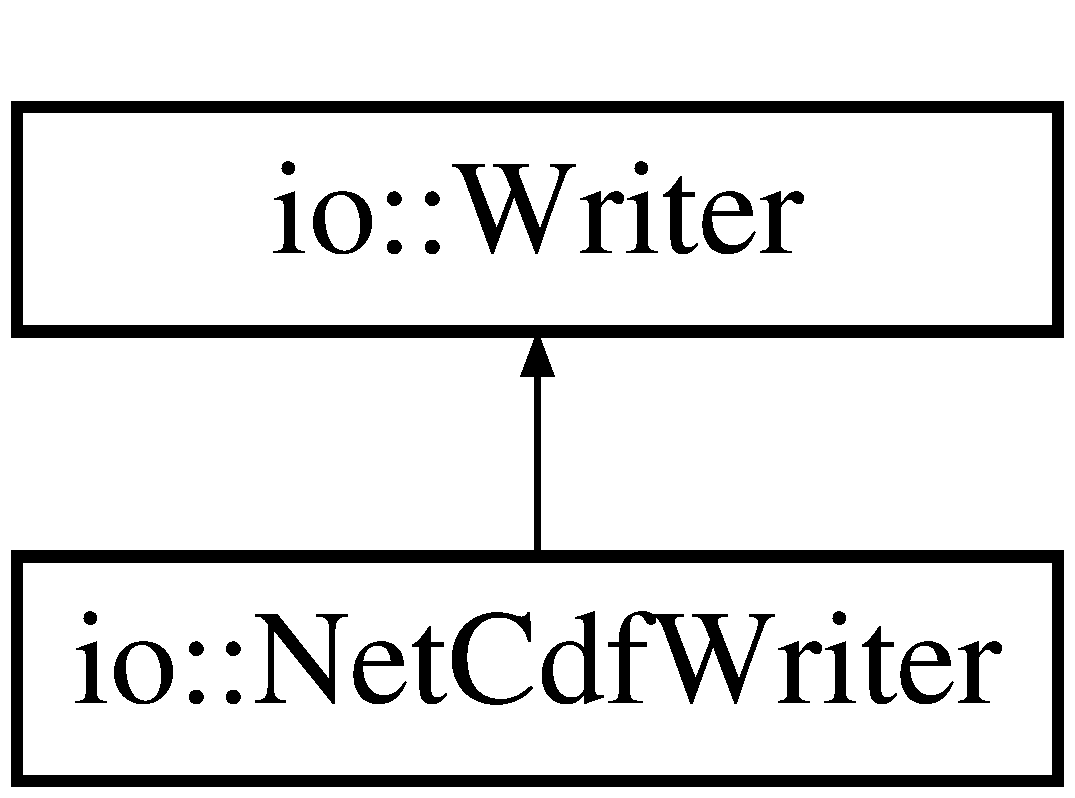
\includegraphics[height=2.000000cm]{classio_1_1NetCdfWriter}
\end{center}
\end{figure}
\subsection*{Public Member Functions}
\begin{DoxyCompactItemize}
\item 
\hyperlink{classio_1_1NetCdfWriter_afb378e970e3f004612cfc36a0c171805}{Net\-Cdf\-Writer} (const std\-::string \&i\-\_\-file\-Name, const \hyperlink{classFloat2D}{Float2\-D} \&i\-\_\-b, const \hyperlink{structio_1_1BoundarySize}{Boundary\-Size} \&i\-\_\-boundary\-Size, int i\-\_\-n\-X, int i\-\_\-n\-Y, float i\-\_\-d\-X, float i\-\_\-d\-Y, float i\-\_\-origin\-X=0., float i\-\_\-origin\-Y=0., unsigned int i\-\_\-flush=0, size\-\_\-t cont\-Timestep=0)
\item 
\hyperlink{classio_1_1NetCdfWriter_af9066dce4d7c62ef038a10e1244085b0}{Net\-Cdf\-Writer} (const std\-::string \&i\-\_\-file\-Name, const \hyperlink{classFloat2D}{Float2\-D} \&i\-\_\-b, const \hyperlink{structio_1_1BoundarySize}{Boundary\-Size} \&i\-\_\-boundary\-Size, const \hyperlink{SWE__Scenario_8hh_af75d5dd7322fa39ed0af4e7839e600f8}{Boundary\-Type} \&boundary\-Type\-Left, const \hyperlink{SWE__Scenario_8hh_af75d5dd7322fa39ed0af4e7839e600f8}{Boundary\-Type} \&boundary\-Type\-Right, const \hyperlink{SWE__Scenario_8hh_af75d5dd7322fa39ed0af4e7839e600f8}{Boundary\-Type} \&boundary\-Type\-Top, const \hyperlink{SWE__Scenario_8hh_af75d5dd7322fa39ed0af4e7839e600f8}{Boundary\-Type} \&boundary\-Type\-Bottom, const float end\-Of\-Simulation, int i\-\_\-n\-X, int i\-\_\-n\-Y, float i\-\_\-d\-X, float i\-\_\-d\-Y, float i\-\_\-origin\-X=0., float i\-\_\-origin\-Y=0., unsigned int i\-\_\-flush=0, bool use\-Checkpoints=false)
\item 
virtual \hyperlink{classio_1_1NetCdfWriter_ace10f1b56bbb4a1b6c2092ed661a1a0d}{$\sim$\-Net\-Cdf\-Writer} ()
\item 
void \hyperlink{classio_1_1NetCdfWriter_a8e49f21f16b1720a348de50485754b0c}{write\-Time\-Step} (const \hyperlink{classFloat2D}{Float2\-D} \&i\-\_\-h, const \hyperlink{classFloat2D}{Float2\-D} \&i\-\_\-hu, const \hyperlink{classFloat2D}{Float2\-D} \&i\-\_\-hv, float i\-\_\-time)
\end{DoxyCompactItemize}
\subsection*{Additional Inherited Members}


\subsection{Constructor \& Destructor Documentation}
\hypertarget{classio_1_1NetCdfWriter_afb378e970e3f004612cfc36a0c171805}{\index{io\-::\-Net\-Cdf\-Writer@{io\-::\-Net\-Cdf\-Writer}!Net\-Cdf\-Writer@{Net\-Cdf\-Writer}}
\index{Net\-Cdf\-Writer@{Net\-Cdf\-Writer}!io::NetCdfWriter@{io\-::\-Net\-Cdf\-Writer}}
\subsubsection[{Net\-Cdf\-Writer}]{\setlength{\rightskip}{0pt plus 5cm}io\-::\-Net\-Cdf\-Writer\-::\-Net\-Cdf\-Writer (
\begin{DoxyParamCaption}
\item[{const std\-::string \&}]{i\-\_\-base\-Name, }
\item[{const {\bf Float2\-D} \&}]{i\-\_\-b, }
\item[{const {\bf Boundary\-Size} \&}]{i\-\_\-boundary\-Size, }
\item[{int}]{i\-\_\-n\-X, }
\item[{int}]{i\-\_\-n\-Y, }
\item[{float}]{i\-\_\-d\-X, }
\item[{float}]{i\-\_\-d\-Y, }
\item[{float}]{i\-\_\-origin\-X = {\ttfamily 0.}, }
\item[{float}]{i\-\_\-origin\-Y = {\ttfamily 0.}, }
\item[{unsigned int}]{i\-\_\-flush = {\ttfamily 0}, }
\item[{size\-\_\-t}]{cont\-Timestep = {\ttfamily 0}}
\end{DoxyParamCaption}
)}}\label{classio_1_1NetCdfWriter_afb378e970e3f004612cfc36a0c171805}
Create a net\-Cdf-\/file Any existing file will be replaced.


\begin{DoxyParams}{Parameters}
{\em i\-\_\-base\-Name} & base name of the net\-C\-D\-F-\/file to which the data will be written to. \\
\hline
{\em i\-\_\-n\-X} & number of cells in the horizontal direction. \\
\hline
{\em i\-\_\-n\-Y} & number of cells in the vertical direction. \\
\hline
{\em i\-\_\-d\-X} & cell size in x-\/direction. \\
\hline
{\em i\-\_\-d\-Y} & cell size in y-\/direction. \\
\hline
{\em i\-\_\-origin\-X} & \\
\hline
{\em i\-\_\-origin\-Y} & \\
\hline
{\em i\-\_\-flush} & If $>$ 0, flush data to disk every i\-\_\-flush write operation \\
\hline
{\em i\-\_\-dynamic\-Bathymetry} & \\
\hline
\end{DoxyParams}
\hypertarget{classio_1_1NetCdfWriter_af9066dce4d7c62ef038a10e1244085b0}{\index{io\-::\-Net\-Cdf\-Writer@{io\-::\-Net\-Cdf\-Writer}!Net\-Cdf\-Writer@{Net\-Cdf\-Writer}}
\index{Net\-Cdf\-Writer@{Net\-Cdf\-Writer}!io::NetCdfWriter@{io\-::\-Net\-Cdf\-Writer}}
\subsubsection[{Net\-Cdf\-Writer}]{\setlength{\rightskip}{0pt plus 5cm}io\-::\-Net\-Cdf\-Writer\-::\-Net\-Cdf\-Writer (
\begin{DoxyParamCaption}
\item[{const std\-::string \&}]{i\-\_\-base\-Name, }
\item[{const {\bf Float2\-D} \&}]{i\-\_\-b, }
\item[{const {\bf Boundary\-Size} \&}]{i\-\_\-boundary\-Size, }
\item[{const {\bf Boundary\-Type} \&}]{i\-\_\-boundary\-Type\-Left, }
\item[{const {\bf Boundary\-Type} \&}]{i\-\_\-boundary\-Type\-Right, }
\item[{const {\bf Boundary\-Type} \&}]{i\-\_\-boundary\-Type\-Top, }
\item[{const {\bf Boundary\-Type} \&}]{i\-\_\-boundary\-Type\-Bottom, }
\item[{const float}]{i\-\_\-end\-Of\-Simulation, }
\item[{int}]{i\-\_\-n\-X, }
\item[{int}]{i\-\_\-n\-Y, }
\item[{float}]{i\-\_\-d\-X, }
\item[{float}]{i\-\_\-d\-Y, }
\item[{float}]{i\-\_\-origin\-X = {\ttfamily 0.}, }
\item[{float}]{i\-\_\-origin\-Y = {\ttfamily 0.}, }
\item[{unsigned int}]{i\-\_\-flush = {\ttfamily 0}, }
\item[{bool}]{use\-Checkpoints = {\ttfamily false}}
\end{DoxyParamCaption}
)}}\label{classio_1_1NetCdfWriter_af9066dce4d7c62ef038a10e1244085b0}
Create a net\-Cdf-\/file Any existing file will be replaced.


\begin{DoxyParams}{Parameters}
{\em i\-\_\-base\-Name} & base name of the net\-C\-D\-F-\/file to which the data will be written to. \\
\hline
{\em i\-\_\-boundary\-Type\-Left} & The boundary type on the Left of the simulation domain \\
\hline
{\em i\-\_\-boundary\-Type\-Right} & The boundary type on the Right of the simulation domain \\
\hline
{\em i\-\_\-boundary\-Type\-Top} & The boundary type on the Top of the simulation domain \\
\hline
{\em i\-\_\-boundary\-Type\-Bottom} & The boundary type on the Bottom of the simulation domain \\
\hline
{\em i\-\_\-end\-Of\-Simulation} & The time when the simulation should end \\
\hline
{\em i\-\_\-n\-X} & number of cells in the horizontal direction. \\
\hline
{\em i\-\_\-n\-Y} & number of cells in the vertical direction. \\
\hline
{\em i\-\_\-d\-X} & cell size in x-\/direction. \\
\hline
{\em i\-\_\-d\-Y} & cell size in y-\/direction. \\
\hline
{\em i\-\_\-origin\-X} & \\
\hline
{\em i\-\_\-origin\-Y} & \\
\hline
{\em i\-\_\-flush} & If $>$ 0, flush data to disk every i\-\_\-flush write operation \\
\hline
{\em i\-\_\-dynamic\-Bathymetry} & \\
\hline
\end{DoxyParams}
\hypertarget{classio_1_1NetCdfWriter_ace10f1b56bbb4a1b6c2092ed661a1a0d}{\index{io\-::\-Net\-Cdf\-Writer@{io\-::\-Net\-Cdf\-Writer}!$\sim$\-Net\-Cdf\-Writer@{$\sim$\-Net\-Cdf\-Writer}}
\index{$\sim$\-Net\-Cdf\-Writer@{$\sim$\-Net\-Cdf\-Writer}!io::NetCdfWriter@{io\-::\-Net\-Cdf\-Writer}}
\subsubsection[{$\sim$\-Net\-Cdf\-Writer}]{\setlength{\rightskip}{0pt plus 5cm}io\-::\-Net\-Cdf\-Writer\-::$\sim$\-Net\-Cdf\-Writer (
\begin{DoxyParamCaption}
{}
\end{DoxyParamCaption}
)\hspace{0.3cm}{\ttfamily [virtual]}}}\label{classio_1_1NetCdfWriter_ace10f1b56bbb4a1b6c2092ed661a1a0d}
Destructor of a net\-C\-D\-F-\/writer. 

\subsection{Member Function Documentation}
\hypertarget{classio_1_1NetCdfWriter_a8e49f21f16b1720a348de50485754b0c}{\index{io\-::\-Net\-Cdf\-Writer@{io\-::\-Net\-Cdf\-Writer}!write\-Time\-Step@{write\-Time\-Step}}
\index{write\-Time\-Step@{write\-Time\-Step}!io::NetCdfWriter@{io\-::\-Net\-Cdf\-Writer}}
\subsubsection[{write\-Time\-Step}]{\setlength{\rightskip}{0pt plus 5cm}void io\-::\-Net\-Cdf\-Writer\-::write\-Time\-Step (
\begin{DoxyParamCaption}
\item[{const {\bf Float2\-D} \&}]{i\-\_\-h, }
\item[{const {\bf Float2\-D} \&}]{i\-\_\-hu, }
\item[{const {\bf Float2\-D} \&}]{i\-\_\-hv, }
\item[{float}]{i\-\_\-time}
\end{DoxyParamCaption}
)\hspace{0.3cm}{\ttfamily [virtual]}}}\label{classio_1_1NetCdfWriter_a8e49f21f16b1720a348de50485754b0c}
Writes the unknwons to a net\-C\-D\-F-\/file (-\/$>$ constructor) with respect to the boundary sizes.

boundary\-Size\mbox{[}0\mbox{]} == left boundary\-Size\mbox{[}1\mbox{]} == right boundary\-Size\mbox{[}2\mbox{]} == bottom boundary\-Size\mbox{[}3\mbox{]} == top


\begin{DoxyParams}{Parameters}
{\em i\-\_\-h} & water heights at a given time step. \\
\hline
{\em i\-\_\-hu} & momentums in x-\/direction at a given time step. \\
\hline
{\em i\-\_\-hv} & momentums in y-\/direction at a given time step. \\
\hline
{\em i\-\_\-boundary\-Size} & size of the boundaries. \\
\hline
{\em i\-\_\-time} & simulation time of the time step. \\
\hline
\end{DoxyParams}


Implements \hyperlink{classio_1_1Writer_a9ac05caa91aca4e79094d6718a2da16c}{io\-::\-Writer}.



The documentation for this class was generated from the following files\-:\begin{DoxyCompactItemize}
\item 
/home/sascha/\-Dokumente/\-Projects/\-Tsun\-Sim/\-S\-W\-E/src/writer/\hyperlink{NetCdfWriter_8hh}{Net\-Cdf\-Writer.\-hh}\item 
/home/sascha/\-Dokumente/\-Projects/\-Tsun\-Sim/\-S\-W\-E/src/writer/\hyperlink{NetCdfWriter_8cpp}{Net\-Cdf\-Writer.\-cpp}\end{DoxyCompactItemize}

\hypertarget{classio_1_1VtkWriter}{\section{io\-:\-:Vtk\-Writer Class Reference}
\label{classio_1_1VtkWriter}\index{io\-::\-Vtk\-Writer@{io\-::\-Vtk\-Writer}}
}
Inheritance diagram for io\-:\-:Vtk\-Writer\-:\begin{figure}[H]
\begin{center}
\leavevmode
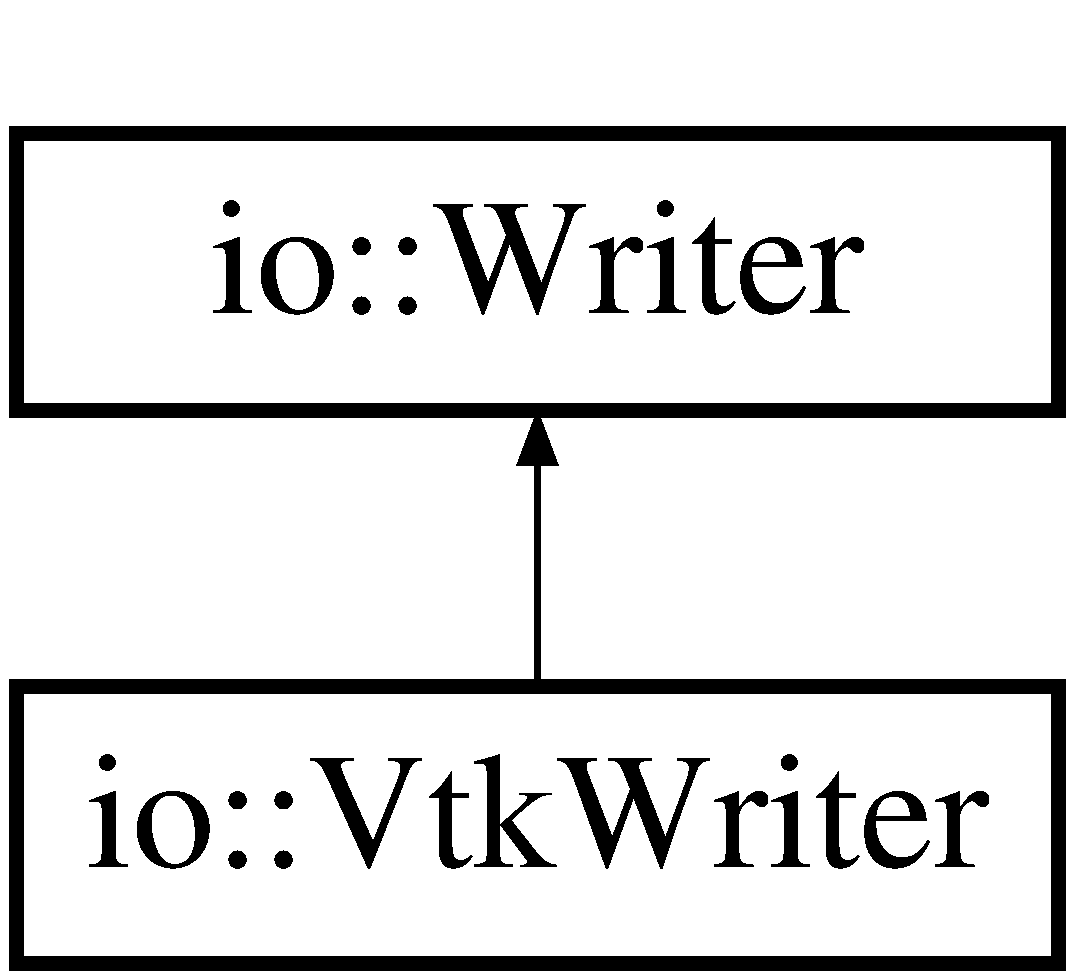
\includegraphics[height=2.000000cm]{classio_1_1VtkWriter}
\end{center}
\end{figure}
\subsection*{Public Member Functions}
\begin{DoxyCompactItemize}
\item 
\hyperlink{classio_1_1VtkWriter_aaed37669d1c38bafaf3fc36169342720}{Vtk\-Writer} (const std\-::string \&i\-\_\-file\-Name, const \hyperlink{classFloat2D}{Float2\-D} \&i\-\_\-b, const \hyperlink{structio_1_1BoundarySize}{Boundary\-Size} \&i\-\_\-boundary\-Size, int i\-\_\-n\-X, int i\-\_\-n\-Y, float i\-\_\-d\-X, float i\-\_\-d\-Y, int i\-\_\-offset\-X=0, int i\-\_\-offset\-Y=0)
\item 
void \hyperlink{classio_1_1VtkWriter_ad464e594a34f4cd94b02087a2fade7bf}{write\-Time\-Step} (const \hyperlink{classFloat2D}{Float2\-D} \&i\-\_\-h, const \hyperlink{classFloat2D}{Float2\-D} \&i\-\_\-hu, const \hyperlink{classFloat2D}{Float2\-D} \&i\-\_\-hv, float i\-\_\-time)
\end{DoxyCompactItemize}
\subsection*{Additional Inherited Members}


\subsection{Constructor \& Destructor Documentation}
\hypertarget{classio_1_1VtkWriter_aaed37669d1c38bafaf3fc36169342720}{\index{io\-::\-Vtk\-Writer@{io\-::\-Vtk\-Writer}!Vtk\-Writer@{Vtk\-Writer}}
\index{Vtk\-Writer@{Vtk\-Writer}!io::VtkWriter@{io\-::\-Vtk\-Writer}}
\subsubsection[{Vtk\-Writer}]{\setlength{\rightskip}{0pt plus 5cm}io\-::\-Vtk\-Writer\-::\-Vtk\-Writer (
\begin{DoxyParamCaption}
\item[{const std\-::string \&}]{i\-\_\-base\-Name, }
\item[{const {\bf Float2\-D} \&}]{i\-\_\-b, }
\item[{const {\bf Boundary\-Size} \&}]{i\-\_\-boundary\-Size, }
\item[{int}]{i\-\_\-n\-X, }
\item[{int}]{i\-\_\-n\-Y, }
\item[{float}]{i\-\_\-d\-X, }
\item[{float}]{i\-\_\-d\-Y, }
\item[{int}]{i\-\_\-offset\-X = {\ttfamily 0}, }
\item[{int}]{i\-\_\-offset\-Y = {\ttfamily 0}}
\end{DoxyParamCaption}
)}}\label{classio_1_1VtkWriter_aaed37669d1c38bafaf3fc36169342720}
Creates a vtk file for each time step. Any existing file will be replaced.


\begin{DoxyParams}{Parameters}
{\em i\-\_\-base\-Name} & base name of the net\-C\-D\-F-\/file to which the data will be written to. \\
\hline
{\em i\-\_\-n\-X} & number of cells in the horizontal direction. \\
\hline
{\em i\-\_\-n\-Y} & number of cells in the vertical direction. \\
\hline
{\em i\-\_\-d\-X} & cell size in x-\/direction. \\
\hline
{\em i\-\_\-d\-Y} & cell size in y-\/direction. \\
\hline
{\em i\-\_\-offset\-X} & x-\/offset of the block \\
\hline
{\em i\-\_\-offset\-Y} & y-\/offset of the block \\
\hline
{\em i\-\_\-dynamic\-Bathymetry} & \\
\hline
\end{DoxyParams}
\begin{DoxyRefDesc}{Todo}
\item[\hyperlink{todo__todo000002}{Todo}]This version can only handle a boundary layer of size 1 \end{DoxyRefDesc}


\subsection{Member Function Documentation}
\hypertarget{classio_1_1VtkWriter_ad464e594a34f4cd94b02087a2fade7bf}{\index{io\-::\-Vtk\-Writer@{io\-::\-Vtk\-Writer}!write\-Time\-Step@{write\-Time\-Step}}
\index{write\-Time\-Step@{write\-Time\-Step}!io::VtkWriter@{io\-::\-Vtk\-Writer}}
\subsubsection[{write\-Time\-Step}]{\setlength{\rightskip}{0pt plus 5cm}void io\-::\-Vtk\-Writer\-::write\-Time\-Step (
\begin{DoxyParamCaption}
\item[{const {\bf Float2\-D} \&}]{i\-\_\-h, }
\item[{const {\bf Float2\-D} \&}]{i\-\_\-hu, }
\item[{const {\bf Float2\-D} \&}]{i\-\_\-hv, }
\item[{float}]{i\-\_\-time}
\end{DoxyParamCaption}
)\hspace{0.3cm}{\ttfamily [virtual]}}}\label{classio_1_1VtkWriter_ad464e594a34f4cd94b02087a2fade7bf}
Writes one time step


\begin{DoxyParams}{Parameters}
{\em i\-\_\-h} & water heights at a given time step. \\
\hline
{\em i\-\_\-hu} & momentums in x-\/direction at a given time step. \\
\hline
{\em i\-\_\-hv} & momentums in y-\/direction at a given time step. \\
\hline
{\em i\-\_\-time} & simulation time of the time step. \\
\hline
\end{DoxyParams}


Implements \hyperlink{classio_1_1Writer_a9ac05caa91aca4e79094d6718a2da16c}{io\-::\-Writer}.



The documentation for this class was generated from the following files\-:\begin{DoxyCompactItemize}
\item 
/home/sascha/\-Dokumente/\-Projects/\-Tsun\-Sim/\-S\-W\-E/src/writer/\hyperlink{VtkWriter_8hh}{Vtk\-Writer.\-hh}\item 
/home/sascha/\-Dokumente/\-Projects/\-Tsun\-Sim/\-S\-W\-E/src/writer/\hyperlink{VtkWriter_8cpp}{Vtk\-Writer.\-cpp}\end{DoxyCompactItemize}

\hypertarget{classio_1_1Writer}{\section{io\-:\-:Writer Class Reference}
\label{classio_1_1Writer}\index{io\-::\-Writer@{io\-::\-Writer}}
}
Inheritance diagram for io\-:\-:Writer\-:\begin{figure}[H]
\begin{center}
\leavevmode
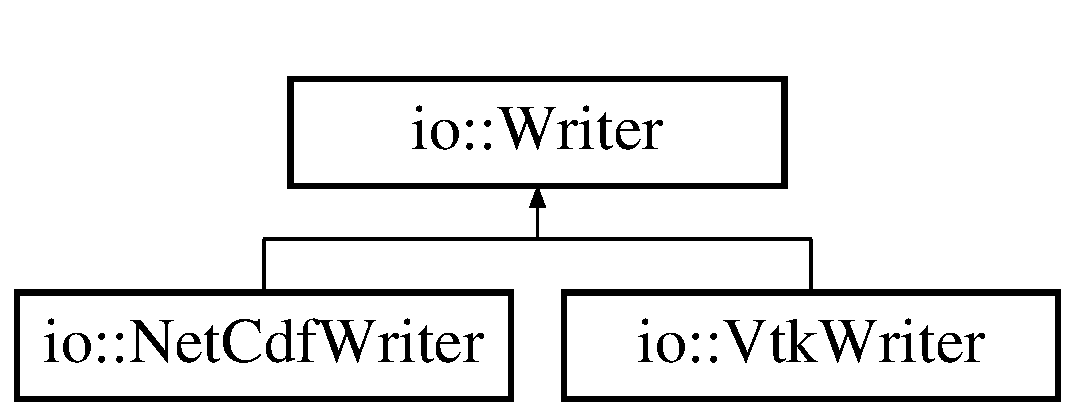
\includegraphics[height=2.000000cm]{classio_1_1Writer}
\end{center}
\end{figure}
\subsection*{Public Member Functions}
\begin{DoxyCompactItemize}
\item 
\hyperlink{classio_1_1Writer_a6fe95f4a66e8b8ee1c9a52196ff3433f}{Writer} (const std\-::string \&i\-\_\-file\-Name, const \hyperlink{classFloat2D}{Float2\-D} \&i\-\_\-b, const \hyperlink{structio_1_1BoundarySize}{Boundary\-Size} \&i\-\_\-boundary\-Size, int i\-\_\-n\-X, int i\-\_\-n\-Y)
\item 
virtual void \hyperlink{classio_1_1Writer_a9ac05caa91aca4e79094d6718a2da16c}{write\-Time\-Step} (const \hyperlink{classFloat2D}{Float2\-D} \&i\-\_\-h, const \hyperlink{classFloat2D}{Float2\-D} \&i\-\_\-hu, const \hyperlink{classFloat2D}{Float2\-D} \&i\-\_\-hv, float i\-\_\-time)=0
\end{DoxyCompactItemize}
\subsection*{Protected Attributes}
\begin{DoxyCompactItemize}
\item 
\hypertarget{classio_1_1Writer_a93b978e8cbfc6bcf6dbfdc3f393d300a}{const std\-::string \hyperlink{classio_1_1Writer_a93b978e8cbfc6bcf6dbfdc3f393d300a}{file\-Name}}\label{classio_1_1Writer_a93b978e8cbfc6bcf6dbfdc3f393d300a}

\begin{DoxyCompactList}\small\item\em file name of the data file \end{DoxyCompactList}\item 
\hypertarget{classio_1_1Writer_a1f5d4ab8728ae1c2ceba52c6c822d0bc}{const \hyperlink{classFloat2D}{Float2\-D} \& \hyperlink{classio_1_1Writer_a1f5d4ab8728ae1c2ceba52c6c822d0bc}{b}}\label{classio_1_1Writer_a1f5d4ab8728ae1c2ceba52c6c822d0bc}

\begin{DoxyCompactList}\small\item\em (Reference) to bathymetry data \end{DoxyCompactList}\item 
\hypertarget{classio_1_1Writer_a7cf701232192c20c41cbb4454601c219}{const \hyperlink{structio_1_1BoundarySize}{Boundary\-Size} \hyperlink{classio_1_1Writer_a7cf701232192c20c41cbb4454601c219}{boundary\-Size}}\label{classio_1_1Writer_a7cf701232192c20c41cbb4454601c219}

\begin{DoxyCompactList}\small\item\em Boundary layer size. \end{DoxyCompactList}\item 
\hypertarget{classio_1_1Writer_a080fc86da3b2d8ea130382917d96252d}{const unsigned int \hyperlink{classio_1_1Writer_a080fc86da3b2d8ea130382917d96252d}{n\-X}}\label{classio_1_1Writer_a080fc86da3b2d8ea130382917d96252d}

\begin{DoxyCompactList}\small\item\em dimensions of the grid in x-\/ and y-\/direction. \end{DoxyCompactList}\item 
\hypertarget{classio_1_1Writer_a8c4ceaedd4b3e571cc4a5cacbcb21604}{const unsigned int {\bfseries n\-Y}}\label{classio_1_1Writer_a8c4ceaedd4b3e571cc4a5cacbcb21604}

\item 
\hypertarget{classio_1_1Writer_aa21f3ee8a54cf9278d711fe4f454f45c}{size\-\_\-t \hyperlink{classio_1_1Writer_aa21f3ee8a54cf9278d711fe4f454f45c}{time\-Step}}\label{classio_1_1Writer_aa21f3ee8a54cf9278d711fe4f454f45c}

\begin{DoxyCompactList}\small\item\em current time step \end{DoxyCompactList}\end{DoxyCompactItemize}


\subsection{Constructor \& Destructor Documentation}
\hypertarget{classio_1_1Writer_a6fe95f4a66e8b8ee1c9a52196ff3433f}{\index{io\-::\-Writer@{io\-::\-Writer}!Writer@{Writer}}
\index{Writer@{Writer}!io::Writer@{io\-::\-Writer}}
\subsubsection[{Writer}]{\setlength{\rightskip}{0pt plus 5cm}io\-::\-Writer\-::\-Writer (
\begin{DoxyParamCaption}
\item[{const std\-::string \&}]{i\-\_\-file\-Name, }
\item[{const {\bf Float2\-D} \&}]{i\-\_\-b, }
\item[{const {\bf Boundary\-Size} \&}]{i\-\_\-boundary\-Size, }
\item[{int}]{i\-\_\-n\-X, }
\item[{int}]{i\-\_\-n\-Y}
\end{DoxyParamCaption}
)\hspace{0.3cm}{\ttfamily [inline]}}}\label{classio_1_1Writer_a6fe95f4a66e8b8ee1c9a52196ff3433f}

\begin{DoxyParams}{Parameters}
{\em i\-\_\-boundary\-Size} & size of the boundaries. \\
\hline
\end{DoxyParams}


\subsection{Member Function Documentation}
\hypertarget{classio_1_1Writer_a9ac05caa91aca4e79094d6718a2da16c}{\index{io\-::\-Writer@{io\-::\-Writer}!write\-Time\-Step@{write\-Time\-Step}}
\index{write\-Time\-Step@{write\-Time\-Step}!io::Writer@{io\-::\-Writer}}
\subsubsection[{write\-Time\-Step}]{\setlength{\rightskip}{0pt plus 5cm}virtual void io\-::\-Writer\-::write\-Time\-Step (
\begin{DoxyParamCaption}
\item[{const {\bf Float2\-D} \&}]{i\-\_\-h, }
\item[{const {\bf Float2\-D} \&}]{i\-\_\-hu, }
\item[{const {\bf Float2\-D} \&}]{i\-\_\-hv, }
\item[{float}]{i\-\_\-time}
\end{DoxyParamCaption}
)\hspace{0.3cm}{\ttfamily [pure virtual]}}}\label{classio_1_1Writer_a9ac05caa91aca4e79094d6718a2da16c}
Writes one time step


\begin{DoxyParams}{Parameters}
{\em i\-\_\-h} & water heights at a given time step. \\
\hline
{\em i\-\_\-hu} & momentums in x-\/direction at a given time step. \\
\hline
{\em i\-\_\-hv} & momentums in y-\/direction at a given time step. \\
\hline
{\em i\-\_\-time} & simulation time of the time step. \\
\hline
\end{DoxyParams}


Implemented in \hyperlink{classio_1_1NetCdfWriter_a8e49f21f16b1720a348de50485754b0c}{io\-::\-Net\-Cdf\-Writer}, and \hyperlink{classio_1_1VtkWriter_ad464e594a34f4cd94b02087a2fade7bf}{io\-::\-Vtk\-Writer}.



The documentation for this class was generated from the following file\-:\begin{DoxyCompactItemize}
\item 
/home/sascha/\-Dokumente/\-Projects/\-Tsun\-Sim/\-S\-W\-E/src/writer/\hyperlink{Writer_8hh}{Writer.\-hh}\end{DoxyCompactItemize}

\hypertarget{classShader}{\section{Shader Class Reference}
\label{classShader}\index{Shader@{Shader}}
}
\subsection*{Public Member Functions}
\begin{DoxyCompactItemize}
\item 
\hyperlink{classShader_a662551e9ee2ac3a0b1658ac929e16c1a}{Shader} (char const $\ast$vertex\-Shader\-File, char const $\ast$fragment\-Shader\-File)
\item 
\hyperlink{classShader_aff01df87e8a102f270b5b135a295e59d}{$\sim$\-Shader} ()
\item 
bool \hyperlink{classShader_af70fd9c2a4bc664dc0dce167cba627e6}{shaders\-Loaded} ()
\item 
void \hyperlink{classShader_a537720c8635f679c74d843d02c2dc98d}{enable\-Shader} ()
\item 
void \hyperlink{classShader_a858693041864f93142536850be5963dd}{disable\-Shader} ()
\item 
G\-Lint \hyperlink{classShader_a348d7c110ee1e4092aaddc50a657112a}{get\-Uniform\-Location} (const char $\ast$name)
\item 
void \hyperlink{classShader_a0c16e2e949cd318bee4dd00d2f73559a}{set\-Uniform} (G\-Lint location, G\-Lfloat value)
\end{DoxyCompactItemize}


\subsection{Constructor \& Destructor Documentation}
\hypertarget{classShader_a662551e9ee2ac3a0b1658ac929e16c1a}{\index{Shader@{Shader}!Shader@{Shader}}
\index{Shader@{Shader}!Shader@{Shader}}
\subsubsection[{Shader}]{\setlength{\rightskip}{0pt plus 5cm}Shader\-::\-Shader (
\begin{DoxyParamCaption}
\item[{char const $\ast$}]{vertex\-Shader\-File, }
\item[{char const $\ast$}]{fragment\-Shader\-File}
\end{DoxyParamCaption}
)}}\label{classShader_a662551e9ee2ac3a0b1658ac929e16c1a}
Constructor. Check whether shaders are supported. If yes, load vertex and fragment shader from textfile into memory and compile


\begin{DoxyParams}{Parameters}
{\em vertex\-Shader\-File} & name of the text file containing the vertex shader code \\
\hline
{\em fragment\-Shader\-File} & name of the text file containing the fragment shader code \\
\hline
\end{DoxyParams}
\hypertarget{classShader_aff01df87e8a102f270b5b135a295e59d}{\index{Shader@{Shader}!$\sim$\-Shader@{$\sim$\-Shader}}
\index{$\sim$\-Shader@{$\sim$\-Shader}!Shader@{Shader}}
\subsubsection[{$\sim$\-Shader}]{\setlength{\rightskip}{0pt plus 5cm}Shader\-::$\sim$\-Shader (
\begin{DoxyParamCaption}
{}
\end{DoxyParamCaption}
)}}\label{classShader_aff01df87e8a102f270b5b135a295e59d}
Destructor. Unload shaders and free resources. 

\subsection{Member Function Documentation}
\hypertarget{classShader_a858693041864f93142536850be5963dd}{\index{Shader@{Shader}!disable\-Shader@{disable\-Shader}}
\index{disable\-Shader@{disable\-Shader}!Shader@{Shader}}
\subsubsection[{disable\-Shader}]{\setlength{\rightskip}{0pt plus 5cm}void Shader\-::disable\-Shader (
\begin{DoxyParamCaption}
{}
\end{DoxyParamCaption}
)}}\label{classShader_a858693041864f93142536850be5963dd}
Restores Open\-G\-L default shaders \hypertarget{classShader_a537720c8635f679c74d843d02c2dc98d}{\index{Shader@{Shader}!enable\-Shader@{enable\-Shader}}
\index{enable\-Shader@{enable\-Shader}!Shader@{Shader}}
\subsubsection[{enable\-Shader}]{\setlength{\rightskip}{0pt plus 5cm}void Shader\-::enable\-Shader (
\begin{DoxyParamCaption}
{}
\end{DoxyParamCaption}
)}}\label{classShader_a537720c8635f679c74d843d02c2dc98d}
Replaces Open\-G\-L shaders by our custom shaders \hypertarget{classShader_a348d7c110ee1e4092aaddc50a657112a}{\index{Shader@{Shader}!get\-Uniform\-Location@{get\-Uniform\-Location}}
\index{get\-Uniform\-Location@{get\-Uniform\-Location}!Shader@{Shader}}
\subsubsection[{get\-Uniform\-Location}]{\setlength{\rightskip}{0pt plus 5cm}G\-Lint Shader\-::get\-Uniform\-Location (
\begin{DoxyParamCaption}
\item[{const char $\ast$}]{name}
\end{DoxyParamCaption}
)\hspace{0.3cm}{\ttfamily [inline]}}}\label{classShader_a348d7c110ee1e4092aaddc50a657112a}
\begin{DoxyReturn}{Returns}
Location of the uniform variable 
\end{DoxyReturn}
\hypertarget{classShader_a0c16e2e949cd318bee4dd00d2f73559a}{\index{Shader@{Shader}!set\-Uniform@{set\-Uniform}}
\index{set\-Uniform@{set\-Uniform}!Shader@{Shader}}
\subsubsection[{set\-Uniform}]{\setlength{\rightskip}{0pt plus 5cm}void Shader\-::set\-Uniform (
\begin{DoxyParamCaption}
\item[{G\-Lint}]{location, }
\item[{G\-Lfloat}]{value}
\end{DoxyParamCaption}
)\hspace{0.3cm}{\ttfamily [inline]}}}\label{classShader_a0c16e2e949cd318bee4dd00d2f73559a}
Set a uniform variable in the shader \hypertarget{classShader_af70fd9c2a4bc664dc0dce167cba627e6}{\index{Shader@{Shader}!shaders\-Loaded@{shaders\-Loaded}}
\index{shaders\-Loaded@{shaders\-Loaded}!Shader@{Shader}}
\subsubsection[{shaders\-Loaded}]{\setlength{\rightskip}{0pt plus 5cm}bool Shader\-::shaders\-Loaded (
\begin{DoxyParamCaption}
{}
\end{DoxyParamCaption}
)}}\label{classShader_af70fd9c2a4bc664dc0dce167cba627e6}
Returns, whether shaders could by loaded successfully 

The documentation for this class was generated from the following files\-:\begin{DoxyCompactItemize}
\item 
/home/sascha/\-Dokumente/\-Projects/\-Tsun\-Sim/\-S\-W\-E/src/opengl/shader.\-h\item 
/home/sascha/\-Dokumente/\-Projects/\-Tsun\-Sim/\-S\-W\-E/src/opengl/shader.\-cpp\end{DoxyCompactItemize}

\hypertarget{classSimulation}{\section{Simulation Class Reference}
\label{classSimulation}\index{Simulation@{Simulation}}
}
\subsection*{Public Member Functions}
\begin{DoxyCompactItemize}
\item 
\hyperlink{classSimulation_a5b224cc5b36bcc8eb29689aff223de41}{Simulation} ()
\item 
\hyperlink{classSimulation_a80fad3f57dfaf195a36f7bc49bc88279}{$\sim$\-Simulation} ()
\item 
void \hyperlink{classSimulation_a6be9990c6b2e31959254c8aa7b6df8a1}{restart} ()
\item 
\hypertarget{classSimulation_a0d9c93f7fbb498ac6f84d22baab8bbb0}{void {\bfseries load\-New\-Scenario} (\hyperlink{classSWE__Scenario}{S\-W\-E\-\_\-\-Scenario} $\ast$scene)}\label{classSimulation_a0d9c93f7fbb498ac6f84d22baab8bbb0}

\item 
\hypertarget{classSimulation_a349cba71f66fac2a159e3517ae7327ab}{void {\bfseries resize} (float factor)}\label{classSimulation_a349cba71f66fac2a159e3517ae7327ab}

\item 
void \hyperlink{classSimulation_a3d8e72877a4c982eaead748b8f8faf36}{set\-Bath\-Buffer} (float $\ast$output)
\item 
void \hyperlink{classSimulation_ab49e788b7f797a1bebdb3f5667cc95b9}{run\-Cuda} (struct cuda\-Graphics\-Resource $\ast$$\ast$vbo\-\_\-resource, struct cuda\-Graphics\-Resource $\ast$$\ast$vbo\-\_\-normals)
\item 
\hypertarget{classSimulation_a3e99b3b75a733fe887f1ea60307af78e}{int {\bfseries get\-Nx} ()}\label{classSimulation_a3e99b3b75a733fe887f1ea60307af78e}

\item 
\hypertarget{classSimulation_a58809b28521e41ba4b853cbf49dcd5a6}{int {\bfseries get\-Ny} ()}\label{classSimulation_a58809b28521e41ba4b853cbf49dcd5a6}

\item 
\hypertarget{classSimulation_a54ff6716f1d6d7a7627ee31062afa2c2}{const \hyperlink{classFloat2D}{Float2\-D} \& {\bfseries get\-Bathymetry} ()}\label{classSimulation_a54ff6716f1d6d7a7627ee31062afa2c2}

\item 
void \hyperlink{classSimulation_aeb1357e23e68821bb27922f3c97b04c2}{get\-Scaling\-Approximation} (float \&b\-Scale, float \&b\-Offset, float \&w\-Scale)
\item 
\hypertarget{classSimulation_a60120697b4c33d63ed3226f30683f207}{void {\bfseries toogle\-Loop} ()}\label{classSimulation_a60120697b4c33d63ed3226f30683f207}

\end{DoxyCompactItemize}


\subsection{Constructor \& Destructor Documentation}
\hypertarget{classSimulation_a5b224cc5b36bcc8eb29689aff223de41}{\index{Simulation@{Simulation}!Simulation@{Simulation}}
\index{Simulation@{Simulation}!Simulation@{Simulation}}
\subsubsection[{Simulation}]{\setlength{\rightskip}{0pt plus 5cm}Simulation\-::\-Simulation (
\begin{DoxyParamCaption}
{}
\end{DoxyParamCaption}
)}}\label{classSimulation_a5b224cc5b36bcc8eb29689aff223de41}
Constructor. Initializes \hyperlink{classSWE__BlockCUDA}{S\-W\-E\-\_\-\-Block\-C\-U\-D\-A} and creates a new instance of it. \hypertarget{classSimulation_a80fad3f57dfaf195a36f7bc49bc88279}{\index{Simulation@{Simulation}!$\sim$\-Simulation@{$\sim$\-Simulation}}
\index{$\sim$\-Simulation@{$\sim$\-Simulation}!Simulation@{Simulation}}
\subsubsection[{$\sim$\-Simulation}]{\setlength{\rightskip}{0pt plus 5cm}Simulation\-::$\sim$\-Simulation (
\begin{DoxyParamCaption}
{}
\end{DoxyParamCaption}
)}}\label{classSimulation_a80fad3f57dfaf195a36f7bc49bc88279}
Destructor. 

\subsection{Member Function Documentation}
\hypertarget{classSimulation_aeb1357e23e68821bb27922f3c97b04c2}{\index{Simulation@{Simulation}!get\-Scaling\-Approximation@{get\-Scaling\-Approximation}}
\index{get\-Scaling\-Approximation@{get\-Scaling\-Approximation}!Simulation@{Simulation}}
\subsubsection[{get\-Scaling\-Approximation}]{\setlength{\rightskip}{0pt plus 5cm}void Simulation\-::get\-Scaling\-Approximation (
\begin{DoxyParamCaption}
\item[{float \&}]{b\-Scale, }
\item[{float \&}]{b\-Offset, }
\item[{float \&}]{w\-Scale}
\end{DoxyParamCaption}
)}}\label{classSimulation_aeb1357e23e68821bb27922f3c97b04c2}
Computes a first approximation of the scaling values needed for visualization. Gets called before simulation starts and determines the average, mininimum and maximum values of the bathymetry and water surface data. Uses latter values to estimate the scaling factors. \hypertarget{classSimulation_a6be9990c6b2e31959254c8aa7b6df8a1}{\index{Simulation@{Simulation}!restart@{restart}}
\index{restart@{restart}!Simulation@{Simulation}}
\subsubsection[{restart}]{\setlength{\rightskip}{0pt plus 5cm}void Simulation\-::restart (
\begin{DoxyParamCaption}
{}
\end{DoxyParamCaption}
)}}\label{classSimulation_a6be9990c6b2e31959254c8aa7b6df8a1}
Restarts the simulation. Restores the initial bondaries. \hypertarget{classSimulation_ab49e788b7f797a1bebdb3f5667cc95b9}{\index{Simulation@{Simulation}!run\-Cuda@{run\-Cuda}}
\index{run\-Cuda@{run\-Cuda}!Simulation@{Simulation}}
\subsubsection[{run\-Cuda}]{\setlength{\rightskip}{0pt plus 5cm}void Simulation\-::run\-Cuda (
\begin{DoxyParamCaption}
\item[{struct cuda\-Graphics\-Resource $\ast$$\ast$}]{vbo\-\_\-resource, }
\item[{struct cuda\-Graphics\-Resource $\ast$$\ast$}]{vbo\-\_\-normals}
\end{DoxyParamCaption}
)}}\label{classSimulation_ab49e788b7f797a1bebdb3f5667cc95b9}
This is the main simulation procedure. Simulates one timestep and computes normals afterwards.


\begin{DoxyParams}{Parameters}
{\em vbo\-\_\-resource} & cuda resource holding the vertex positions \\
\hline
{\em vbo\-\_\-normals} & cuda resource holding the normals \\
\hline
\end{DoxyParams}
\hypertarget{classSimulation_a3d8e72877a4c982eaead748b8f8faf36}{\index{Simulation@{Simulation}!set\-Bath\-Buffer@{set\-Bath\-Buffer}}
\index{set\-Bath\-Buffer@{set\-Bath\-Buffer}!Simulation@{Simulation}}
\subsubsection[{set\-Bath\-Buffer}]{\setlength{\rightskip}{0pt plus 5cm}void Simulation\-::set\-Bath\-Buffer (
\begin{DoxyParamCaption}
\item[{float $\ast$}]{bath}
\end{DoxyParamCaption}
)}}\label{classSimulation_a3d8e72877a4c982eaead748b8f8faf36}
Sets the bathymetry buffer. Buffer contains vertex position and vertex normal in sequence. 
\begin{DoxyParams}{Parameters}
{\em bath} & float array in which computed values will be stored \\
\hline
\end{DoxyParams}


The documentation for this class was generated from the following files\-:\begin{DoxyCompactItemize}
\item 
src/opengl/simulation.\-h\item 
src/opengl/simulation.\-cu\end{DoxyCompactItemize}

\hypertarget{classsolver_1_1FWave}{\section{solver\-:\-:F\-Wave$<$ T $>$ Class Template Reference}
\label{classsolver_1_1FWave}\index{solver\-::\-F\-Wave$<$ T $>$@{solver\-::\-F\-Wave$<$ T $>$}}
}


{\ttfamily \#include $<$F\-Wave.\-hpp$>$}

\subsection*{Public Member Functions}
\begin{DoxyCompactItemize}
\item 
\hyperlink{classsolver_1_1FWave_a446e2721d799afa5612a3a2b8c30d668}{F\-Wave} ()
\item 
\hypertarget{classsolver_1_1FWave_ac300b35d491bfc9ff591c79115017042}{{\bfseries F\-Wave} (bool use\-Outflow)}\label{classsolver_1_1FWave_ac300b35d491bfc9ff591c79115017042}

\item 
void \hyperlink{classsolver_1_1FWave_afb800cb94c48af043ac828c9d730ae63}{compute\-Net\-Updates} (T i\-\_\-h\-\_\-l, T i\-\_\-h\-\_\-r, T i\-\_\-hu\-\_\-l, T i\-\_\-hu\-\_\-r, T i\-\_\-b\-\_\-l, T i\-\_\-b\-\_\-r, T \&o\-\_\-h\-\_\-l, T \&o\-\_\-h\-\_\-r, T \&o\-\_\-hu\-\_\-l, T \&o\-\_\-hu\-\_\-r, T \&o\-\_\-max\-\_\-ws)
\end{DoxyCompactItemize}


\subsection{Detailed Description}
\subsubsection*{template$<$typename T$>$class solver\-::\-F\-Wave$<$ T $>$}

Simple solver used to compute net udates for a given set of height, momentum and bathymetry values 

\subsection{Constructor \& Destructor Documentation}
\hypertarget{classsolver_1_1FWave_a446e2721d799afa5612a3a2b8c30d668}{\index{solver\-::\-F\-Wave@{solver\-::\-F\-Wave}!F\-Wave@{F\-Wave}}
\index{F\-Wave@{F\-Wave}!solver::FWave@{solver\-::\-F\-Wave}}
\subsubsection[{F\-Wave}]{\setlength{\rightskip}{0pt plus 5cm}template$<$typename T$>$ {\bf solver\-::\-F\-Wave}$<$ T $>$\-::{\bf F\-Wave} (
\begin{DoxyParamCaption}
{}
\end{DoxyParamCaption}
)\hspace{0.3cm}{\ttfamily [inline]}}}\label{classsolver_1_1FWave_a446e2721d799afa5612a3a2b8c30d668}
The default constructor just setting gravity 

\subsection{Member Function Documentation}
\hypertarget{classsolver_1_1FWave_afb800cb94c48af043ac828c9d730ae63}{\index{solver\-::\-F\-Wave@{solver\-::\-F\-Wave}!compute\-Net\-Updates@{compute\-Net\-Updates}}
\index{compute\-Net\-Updates@{compute\-Net\-Updates}!solver::FWave@{solver\-::\-F\-Wave}}
\subsubsection[{compute\-Net\-Updates}]{\setlength{\rightskip}{0pt plus 5cm}template$<$typename T$>$ void {\bf solver\-::\-F\-Wave}$<$ T $>$\-::compute\-Net\-Updates (
\begin{DoxyParamCaption}
\item[{T}]{i\-\_\-h\-\_\-l, }
\item[{T}]{i\-\_\-h\-\_\-r, }
\item[{T}]{i\-\_\-hu\-\_\-l, }
\item[{T}]{i\-\_\-hu\-\_\-r, }
\item[{T}]{i\-\_\-b\-\_\-l, }
\item[{T}]{i\-\_\-b\-\_\-r, }
\item[{T \&}]{o\-\_\-h\-\_\-l, }
\item[{T \&}]{o\-\_\-h\-\_\-r, }
\item[{T \&}]{o\-\_\-hu\-\_\-l, }
\item[{T \&}]{o\-\_\-hu\-\_\-r, }
\item[{T \&}]{o\-\_\-max\-\_\-ws}
\end{DoxyParamCaption}
)\hspace{0.3cm}{\ttfamily [inline]}}}\label{classsolver_1_1FWave_afb800cb94c48af043ac828c9d730ae63}
Computes the next timesteps net updates


\begin{DoxyParams}{Parameters}
{\em i\-\_\-h\-\_\-l} & the height on the left cell of the edge \\
\hline
{\em i\-\_\-h\-\_\-r} & the height on the right cell of the edge \\
\hline
{\em i\-\_\-hu\-\_\-l} & the momentum on the left cell of the edge \\
\hline
{\em i\-\_\-hu\-\_\-r} & the momentum on the right cell of the edge \\
\hline
{\em i\-\_\-b\-\_\-l} & the bathymetry on the left cell of the edge \\
\hline
{\em i\-\_\-b\-\_\-r} & the bathymetry on the right cell of the edge\\
\hline
{\em o\-\_\-h\-\_\-l} & output\-: the height update for the left cell \\
\hline
{\em o\-\_\-h\-\_\-r} & output\-: the height update for the right cell \\
\hline
{\em o\-\_\-hu\-\_\-l} & output\-: the momentum update for the left cell \\
\hline
{\em o\-\_\-hu\-\_\-r} & output\-: the momentum update for the right cell \\
\hline
{\em o\-\_\-max\-\_\-wd} & output\-: the maximum wavespeed (which is the maximum of the left and right wave speed) \\
\hline
\end{DoxyParams}


The documentation for this class was generated from the following file\-:\begin{DoxyCompactItemize}
\item 
/home/sascha/\-Dokumente/\-Projects/\-Tsun\-Sim/\-S\-W\-E/submodules/swe\-\_\-solvers/F\-Wave.\-hpp\end{DoxyCompactItemize}

\hypertarget{classSWE__AsagiGrid}{\section{S\-W\-E\-\_\-\-Asagi\-Grid Class Reference}
\label{classSWE__AsagiGrid}\index{S\-W\-E\-\_\-\-Asagi\-Grid@{S\-W\-E\-\_\-\-Asagi\-Grid}}
}
\subsection*{Public Member Functions}
\begin{DoxyCompactItemize}
\item 
\hypertarget{classSWE__AsagiGrid_a36c68a45fd51ed1bae1971ac252ed1cc}{void {\bfseries open} (const std\-::string \&i\-\_\-filename)}\label{classSWE__AsagiGrid_a36c68a45fd51ed1bae1971ac252ed1cc}

\item 
\hypertarget{classSWE__AsagiGrid_ab0dca1af30b0d89f3a68f429c77b0840}{void {\bfseries close} ()}\label{classSWE__AsagiGrid_ab0dca1af30b0d89f3a68f429c77b0840}

\item 
\hypertarget{classSWE__AsagiGrid_a8596fb0fdadd3ab51760d7101d6e89d1}{asagi\-::\-Grid \& {\bfseries grid} ()}\label{classSWE__AsagiGrid_a8596fb0fdadd3ab51760d7101d6e89d1}

\end{DoxyCompactItemize}


The documentation for this class was generated from the following file\-:\begin{DoxyCompactItemize}
\item 
/home/sascha/\-Dokumente/\-Projects/\-Tsun\-Sim/\-S\-W\-E/src/scenarios/\hyperlink{SWE__AsagiScenario_8hh}{S\-W\-E\-\_\-\-Asagi\-Scenario.\-hh}\end{DoxyCompactItemize}

\hypertarget{classSWE__AsagiJapanSmallVisInfo}{\section{S\-W\-E\-\_\-\-Asagi\-Japan\-Small\-Vis\-Info Class Reference}
\label{classSWE__AsagiJapanSmallVisInfo}\index{S\-W\-E\-\_\-\-Asagi\-Japan\-Small\-Vis\-Info@{S\-W\-E\-\_\-\-Asagi\-Japan\-Small\-Vis\-Info}}
}
Inheritance diagram for S\-W\-E\-\_\-\-Asagi\-Japan\-Small\-Vis\-Info\-:\begin{figure}[H]
\begin{center}
\leavevmode
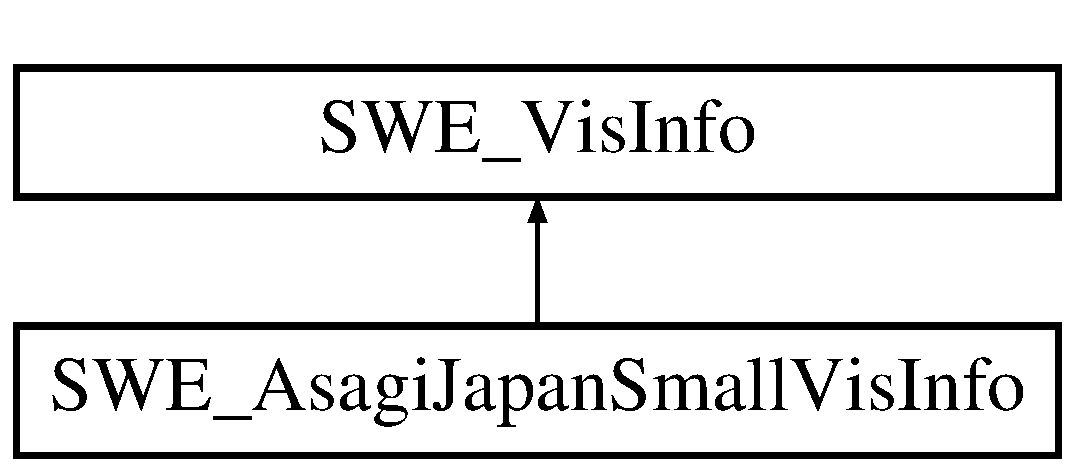
\includegraphics[height=2.000000cm]{classSWE__AsagiJapanSmallVisInfo}
\end{center}
\end{figure}
\subsection*{Public Member Functions}
\begin{DoxyCompactItemize}
\item 
virtual float \hyperlink{classSWE__AsagiJapanSmallVisInfo_a9c2092b5e02596e5ca2ba57c39d3b77e}{water\-Vertical\-Scaling} ()
\item 
virtual float \hyperlink{classSWE__AsagiJapanSmallVisInfo_ab25d85575460a76d88b90e2c927d49ac}{bathy\-Vertical\-Scaling} ()
\end{DoxyCompactItemize}


\subsection{Member Function Documentation}
\hypertarget{classSWE__AsagiJapanSmallVisInfo_ab25d85575460a76d88b90e2c927d49ac}{\index{S\-W\-E\-\_\-\-Asagi\-Japan\-Small\-Vis\-Info@{S\-W\-E\-\_\-\-Asagi\-Japan\-Small\-Vis\-Info}!bathy\-Vertical\-Scaling@{bathy\-Vertical\-Scaling}}
\index{bathy\-Vertical\-Scaling@{bathy\-Vertical\-Scaling}!SWE_AsagiJapanSmallVisInfo@{S\-W\-E\-\_\-\-Asagi\-Japan\-Small\-Vis\-Info}}
\subsubsection[{bathy\-Vertical\-Scaling}]{\setlength{\rightskip}{0pt plus 5cm}virtual float S\-W\-E\-\_\-\-Asagi\-Japan\-Small\-Vis\-Info\-::bathy\-Vertical\-Scaling (
\begin{DoxyParamCaption}
{}
\end{DoxyParamCaption}
)\hspace{0.3cm}{\ttfamily [inline]}, {\ttfamily [virtual]}}}\label{classSWE__AsagiJapanSmallVisInfo_ab25d85575460a76d88b90e2c927d49ac}
\begin{DoxyReturn}{Returns}
The vertical scaling factor for the bathymetry 
\end{DoxyReturn}


Reimplemented from \hyperlink{classSWE__VisInfo_a10ddd7a192e67c69832e695e48b26e91}{S\-W\-E\-\_\-\-Vis\-Info}.

\hypertarget{classSWE__AsagiJapanSmallVisInfo_a9c2092b5e02596e5ca2ba57c39d3b77e}{\index{S\-W\-E\-\_\-\-Asagi\-Japan\-Small\-Vis\-Info@{S\-W\-E\-\_\-\-Asagi\-Japan\-Small\-Vis\-Info}!water\-Vertical\-Scaling@{water\-Vertical\-Scaling}}
\index{water\-Vertical\-Scaling@{water\-Vertical\-Scaling}!SWE_AsagiJapanSmallVisInfo@{S\-W\-E\-\_\-\-Asagi\-Japan\-Small\-Vis\-Info}}
\subsubsection[{water\-Vertical\-Scaling}]{\setlength{\rightskip}{0pt plus 5cm}virtual float S\-W\-E\-\_\-\-Asagi\-Japan\-Small\-Vis\-Info\-::water\-Vertical\-Scaling (
\begin{DoxyParamCaption}
{}
\end{DoxyParamCaption}
)\hspace{0.3cm}{\ttfamily [inline]}, {\ttfamily [virtual]}}}\label{classSWE__AsagiJapanSmallVisInfo_a9c2092b5e02596e5ca2ba57c39d3b77e}
\begin{DoxyReturn}{Returns}
The vertical scaling factor of the water 
\end{DoxyReturn}


Reimplemented from \hyperlink{classSWE__VisInfo_a9552a55a7581b7835d415315e2c17f04}{S\-W\-E\-\_\-\-Vis\-Info}.



The documentation for this class was generated from the following file\-:\begin{DoxyCompactItemize}
\item 
src/scenarios/\hyperlink{SWE__AsagiScenario__vis_8hh}{S\-W\-E\-\_\-\-Asagi\-Scenario\-\_\-vis.\-hh}\end{DoxyCompactItemize}

\hypertarget{classSWE__AsagiScenario}{\section{S\-W\-E\-\_\-\-Asagi\-Scenario Class Reference}
\label{classSWE__AsagiScenario}\index{S\-W\-E\-\_\-\-Asagi\-Scenario@{S\-W\-E\-\_\-\-Asagi\-Scenario}}
}
Inheritance diagram for S\-W\-E\-\_\-\-Asagi\-Scenario\-:\begin{figure}[H]
\begin{center}
\leavevmode
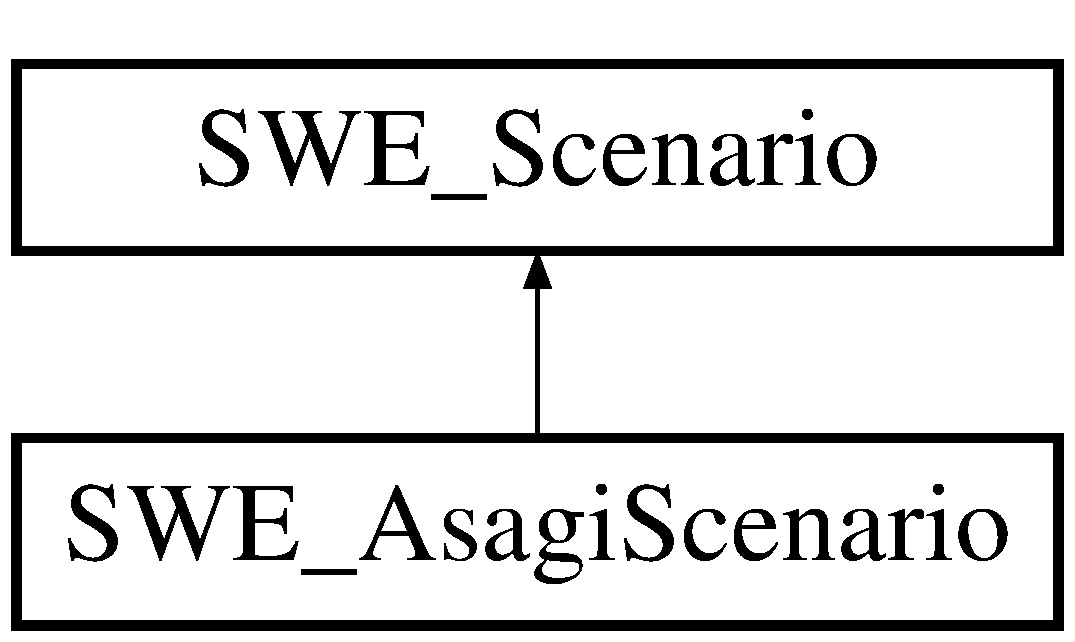
\includegraphics[height=2.000000cm]{classSWE__AsagiScenario}
\end{center}
\end{figure}
\subsection*{Public Member Functions}
\begin{DoxyCompactItemize}
\item 
\hyperlink{classSWE__AsagiScenario_a9add0345b6793da297a44598451074e1}{S\-W\-E\-\_\-\-Asagi\-Scenario} (const std\-::string i\-\_\-bathymetry\-File, const std\-::string i\-\_\-displacement\-File, const float i\-\_\-duration, const float i\-\_\-simulation\-Area\mbox{[}4\mbox{]}, const bool i\-\_\-dynamic\-Displacement=false)
\item 
\hypertarget{classSWE__AsagiScenario_a48d6ba2326cbc06df693990cf41144e6}{void {\bfseries delete\-Grids} ()}\label{classSWE__AsagiScenario_a48d6ba2326cbc06df693990cf41144e6}

\item 
float \hyperlink{classSWE__AsagiScenario_a3d2772883dc584cb1c8ffaafa4dafb8f}{get\-Water\-Height} (float i\-\_\-position\-X, float i\-\_\-position\-Y)
\item 
float \hyperlink{classSWE__AsagiScenario_a95456b79bd1f96120bd8efa73d927568}{get\-Bathymetry} (const float i\-\_\-position\-X, const float i\-\_\-position\-Y)
\item 
float \hyperlink{classSWE__AsagiScenario_a462a4df01aec18b2e5af37f42e86cfde}{get\-Bathymetry\-And\-Dynamic\-Displacement} (const float i\-\_\-position\-X, const float i\-\_\-position\-Y, const float i\-\_\-time)
\item 
bool \hyperlink{classSWE__AsagiScenario_ada067ab5b456f445c66b9fe84c3a4ca5}{dynamic\-Displacement\-Available} (const float i\-\_\-time)
\item 
float \hyperlink{classSWE__AsagiScenario_a44449cbcfad023f60ae2af020576fe4b}{end\-Simulation} ()
\item 
\hyperlink{SWE__Scenario_8hh_af75d5dd7322fa39ed0af4e7839e600f8}{Boundary\-Type} \hyperlink{classSWE__AsagiScenario_adf7992278300b2cb2475398245bad877}{get\-Boundary\-Type} (\hyperlink{SWE__Scenario_8hh_aa5e01e3f7df312f7b9b0d02521141fcc}{Boundary\-Edge} i\-\_\-edge)
\item 
float \hyperlink{classSWE__AsagiScenario_a1f35638db4394f05fa2d0669634aa9ca}{get\-Boundary\-Pos} (\hyperlink{SWE__Scenario_8hh_aa5e01e3f7df312f7b9b0d02521141fcc}{Boundary\-Edge} i\-\_\-edge)
\end{DoxyCompactItemize}


\subsection{Constructor \& Destructor Documentation}
\hypertarget{classSWE__AsagiScenario_a9add0345b6793da297a44598451074e1}{\index{S\-W\-E\-\_\-\-Asagi\-Scenario@{S\-W\-E\-\_\-\-Asagi\-Scenario}!S\-W\-E\-\_\-\-Asagi\-Scenario@{S\-W\-E\-\_\-\-Asagi\-Scenario}}
\index{S\-W\-E\-\_\-\-Asagi\-Scenario@{S\-W\-E\-\_\-\-Asagi\-Scenario}!SWE_AsagiScenario@{S\-W\-E\-\_\-\-Asagi\-Scenario}}
\subsubsection[{S\-W\-E\-\_\-\-Asagi\-Scenario}]{\setlength{\rightskip}{0pt plus 5cm}S\-W\-E\-\_\-\-Asagi\-Scenario\-::\-S\-W\-E\-\_\-\-Asagi\-Scenario (
\begin{DoxyParamCaption}
\item[{const std\-::string}]{i\-\_\-bathymetry\-File, }
\item[{const std\-::string}]{i\-\_\-displacement\-File, }
\item[{const float}]{i\-\_\-duration, }
\item[{const float}]{i\-\_\-simulation\-Area\mbox{[}4\mbox{]}, }
\item[{const bool}]{i\-\_\-dynamic\-Displacement = {\ttfamily false}}
\end{DoxyParamCaption}
)\hspace{0.3cm}{\ttfamily [inline]}}}\label{classSWE__AsagiScenario_a9add0345b6793da297a44598451074e1}
Constructor of an Asagi Scenario, which initializes the corresponding Asagi grids.


\begin{DoxyParams}{Parameters}
{\em i\-\_\-origin\-X} & origin of the simulation area (x-\/direction) \\
\hline
{\em i\-\_\-origin\-Y} & origin of the simulation area (y-\/direction) \\
\hline
{\em i\-\_\-bathymetry\-File} & path to the net\-C\-D\-F-\/bathymetry file \\
\hline
{\em i\-\_\-displacement\-File} & path to the net\-C\-D\-F-\/displacement file \\
\hline
{\em i\-\_\-duration} & time the simulation runs (in seconds) \\
\hline
\end{DoxyParams}


\subsection{Member Function Documentation}
\hypertarget{classSWE__AsagiScenario_ada067ab5b456f445c66b9fe84c3a4ca5}{\index{S\-W\-E\-\_\-\-Asagi\-Scenario@{S\-W\-E\-\_\-\-Asagi\-Scenario}!dynamic\-Displacement\-Available@{dynamic\-Displacement\-Available}}
\index{dynamic\-Displacement\-Available@{dynamic\-Displacement\-Available}!SWE_AsagiScenario@{S\-W\-E\-\_\-\-Asagi\-Scenario}}
\subsubsection[{dynamic\-Displacement\-Available}]{\setlength{\rightskip}{0pt plus 5cm}bool S\-W\-E\-\_\-\-Asagi\-Scenario\-::dynamic\-Displacement\-Available (
\begin{DoxyParamCaption}
\item[{const float}]{i\-\_\-time}
\end{DoxyParamCaption}
)\hspace{0.3cm}{\ttfamily [inline]}}}\label{classSWE__AsagiScenario_ada067ab5b456f445c66b9fe84c3a4ca5}
Check if there is an dynamic displacement is available for the corresponding time. 
\begin{DoxyParams}{Parameters}
{\em i\-\_\-time} & current simulation time \\
\hline
\end{DoxyParams}
\begin{DoxyReturn}{Returns}
true if there is data available, false else 
\end{DoxyReturn}
\hypertarget{classSWE__AsagiScenario_a44449cbcfad023f60ae2af020576fe4b}{\index{S\-W\-E\-\_\-\-Asagi\-Scenario@{S\-W\-E\-\_\-\-Asagi\-Scenario}!end\-Simulation@{end\-Simulation}}
\index{end\-Simulation@{end\-Simulation}!SWE_AsagiScenario@{S\-W\-E\-\_\-\-Asagi\-Scenario}}
\subsubsection[{end\-Simulation}]{\setlength{\rightskip}{0pt plus 5cm}float S\-W\-E\-\_\-\-Asagi\-Scenario\-::end\-Simulation (
\begin{DoxyParamCaption}
{}
\end{DoxyParamCaption}
)\hspace{0.3cm}{\ttfamily [inline]}, {\ttfamily [virtual]}}}\label{classSWE__AsagiScenario_a44449cbcfad023f60ae2af020576fe4b}
Get the number of seconds, the simulation should run. \begin{DoxyReturn}{Returns}
number of seconds, the simulation should run 
\end{DoxyReturn}


Reimplemented from \hyperlink{classSWE__Scenario}{S\-W\-E\-\_\-\-Scenario}.

\hypertarget{classSWE__AsagiScenario_a95456b79bd1f96120bd8efa73d927568}{\index{S\-W\-E\-\_\-\-Asagi\-Scenario@{S\-W\-E\-\_\-\-Asagi\-Scenario}!get\-Bathymetry@{get\-Bathymetry}}
\index{get\-Bathymetry@{get\-Bathymetry}!SWE_AsagiScenario@{S\-W\-E\-\_\-\-Asagi\-Scenario}}
\subsubsection[{get\-Bathymetry}]{\setlength{\rightskip}{0pt plus 5cm}float S\-W\-E\-\_\-\-Asagi\-Scenario\-::get\-Bathymetry (
\begin{DoxyParamCaption}
\item[{const float}]{i\-\_\-position\-X, }
\item[{const float}]{i\-\_\-position\-Y}
\end{DoxyParamCaption}
)\hspace{0.3cm}{\ttfamily [inline]}, {\ttfamily [virtual]}}}\label{classSWE__AsagiScenario_a95456b79bd1f96120bd8efa73d927568}
Get the bathymetry including static displacement at a specific location


\begin{DoxyParams}{Parameters}
{\em i\-\_\-position\-X} & position relative to the origin of the displacement grid in x-\/direction \\
\hline
{\em i\-\_\-position\-Y} & position relative to the origin of the displacement grid in y-\/direction \\
\hline
\end{DoxyParams}
\begin{DoxyReturn}{Returns}
bathymetry (after the initial displacement (static displacement) 
\end{DoxyReturn}


Reimplemented from \hyperlink{classSWE__Scenario}{S\-W\-E\-\_\-\-Scenario}.

\hypertarget{classSWE__AsagiScenario_a462a4df01aec18b2e5af37f42e86cfde}{\index{S\-W\-E\-\_\-\-Asagi\-Scenario@{S\-W\-E\-\_\-\-Asagi\-Scenario}!get\-Bathymetry\-And\-Dynamic\-Displacement@{get\-Bathymetry\-And\-Dynamic\-Displacement}}
\index{get\-Bathymetry\-And\-Dynamic\-Displacement@{get\-Bathymetry\-And\-Dynamic\-Displacement}!SWE_AsagiScenario@{S\-W\-E\-\_\-\-Asagi\-Scenario}}
\subsubsection[{get\-Bathymetry\-And\-Dynamic\-Displacement}]{\setlength{\rightskip}{0pt plus 5cm}float S\-W\-E\-\_\-\-Asagi\-Scenario\-::get\-Bathymetry\-And\-Dynamic\-Displacement (
\begin{DoxyParamCaption}
\item[{const float}]{i\-\_\-position\-X, }
\item[{const float}]{i\-\_\-position\-Y, }
\item[{const float}]{i\-\_\-time}
\end{DoxyParamCaption}
)\hspace{0.3cm}{\ttfamily [inline]}}}\label{classSWE__AsagiScenario_a462a4df01aec18b2e5af37f42e86cfde}
Get the bathymetry including dynamic displacement at a specific location


\begin{DoxyParams}{Parameters}
{\em i\-\_\-position\-X} & position relative to the origin of the displacement grid in x-\/direction \\
\hline
{\em i\-\_\-position\-Y} & position relative to the origin of the displacement grid in y-\/direction \\
\hline
{\em i\-\_\-time} & time relative to the origin of the dynamic displacement \\
\hline
\end{DoxyParams}
\begin{DoxyReturn}{Returns}
bathymetry (after the initial displacement (static displacement), after the specified amount of time (dynamic displacement)) 
\end{DoxyReturn}
\hypertarget{classSWE__AsagiScenario_a1f35638db4394f05fa2d0669634aa9ca}{\index{S\-W\-E\-\_\-\-Asagi\-Scenario@{S\-W\-E\-\_\-\-Asagi\-Scenario}!get\-Boundary\-Pos@{get\-Boundary\-Pos}}
\index{get\-Boundary\-Pos@{get\-Boundary\-Pos}!SWE_AsagiScenario@{S\-W\-E\-\_\-\-Asagi\-Scenario}}
\subsubsection[{get\-Boundary\-Pos}]{\setlength{\rightskip}{0pt plus 5cm}float S\-W\-E\-\_\-\-Asagi\-Scenario\-::get\-Boundary\-Pos (
\begin{DoxyParamCaption}
\item[{{\bf Boundary\-Edge}}]{i\-\_\-edge}
\end{DoxyParamCaption}
)\hspace{0.3cm}{\ttfamily [inline]}, {\ttfamily [virtual]}}}\label{classSWE__AsagiScenario_a1f35638db4394f05fa2d0669634aa9ca}
Get the boundary positions


\begin{DoxyParams}{Parameters}
{\em i\-\_\-edge} & which edge \\
\hline
\end{DoxyParams}
\begin{DoxyReturn}{Returns}
value in the corresponding dimension 
\end{DoxyReturn}


Reimplemented from \hyperlink{classSWE__Scenario}{S\-W\-E\-\_\-\-Scenario}.

\hypertarget{classSWE__AsagiScenario_adf7992278300b2cb2475398245bad877}{\index{S\-W\-E\-\_\-\-Asagi\-Scenario@{S\-W\-E\-\_\-\-Asagi\-Scenario}!get\-Boundary\-Type@{get\-Boundary\-Type}}
\index{get\-Boundary\-Type@{get\-Boundary\-Type}!SWE_AsagiScenario@{S\-W\-E\-\_\-\-Asagi\-Scenario}}
\subsubsection[{get\-Boundary\-Type}]{\setlength{\rightskip}{0pt plus 5cm}{\bf Boundary\-Type} S\-W\-E\-\_\-\-Asagi\-Scenario\-::get\-Boundary\-Type (
\begin{DoxyParamCaption}
\item[{{\bf Boundary\-Edge}}]{i\-\_\-edge}
\end{DoxyParamCaption}
)\hspace{0.3cm}{\ttfamily [inline]}, {\ttfamily [virtual]}}}\label{classSWE__AsagiScenario_adf7992278300b2cb2475398245bad877}
Get the boundary types of the simulation 
\begin{DoxyParams}{Parameters}
{\em edge} & specific edge \\
\hline
\end{DoxyParams}
\begin{DoxyReturn}{Returns}
type of the edge 
\end{DoxyReturn}


Reimplemented from \hyperlink{classSWE__Scenario}{S\-W\-E\-\_\-\-Scenario}.

\hypertarget{classSWE__AsagiScenario_a3d2772883dc584cb1c8ffaafa4dafb8f}{\index{S\-W\-E\-\_\-\-Asagi\-Scenario@{S\-W\-E\-\_\-\-Asagi\-Scenario}!get\-Water\-Height@{get\-Water\-Height}}
\index{get\-Water\-Height@{get\-Water\-Height}!SWE_AsagiScenario@{S\-W\-E\-\_\-\-Asagi\-Scenario}}
\subsubsection[{get\-Water\-Height}]{\setlength{\rightskip}{0pt plus 5cm}float S\-W\-E\-\_\-\-Asagi\-Scenario\-::get\-Water\-Height (
\begin{DoxyParamCaption}
\item[{float}]{i\-\_\-position\-X, }
\item[{float}]{i\-\_\-position\-Y}
\end{DoxyParamCaption}
)\hspace{0.3cm}{\ttfamily [inline]}, {\ttfamily [virtual]}}}\label{classSWE__AsagiScenario_a3d2772883dc584cb1c8ffaafa4dafb8f}
Get the water height at a specific location (before the initial displacement).


\begin{DoxyParams}{Parameters}
{\em i\-\_\-position\-X} & position relative to the origin of the bathymetry grid in x-\/direction \\
\hline
{\em i\-\_\-position\-Y} & position relative to the origin of the bathymetry grid in y-\/direction \\
\hline
\end{DoxyParams}
\begin{DoxyReturn}{Returns}
water height (before the initial displacement) 
\end{DoxyReturn}


Reimplemented from \hyperlink{classSWE__Scenario}{S\-W\-E\-\_\-\-Scenario}.



The documentation for this class was generated from the following files\-:\begin{DoxyCompactItemize}
\item 
/home/sascha/\-Dokumente/\-Projects/\-Tsun\-Sim/\-S\-W\-E/src/scenarios/\hyperlink{SWE__AsagiScenario_8hh}{S\-W\-E\-\_\-\-Asagi\-Scenario.\-hh}\item 
/home/sascha/\-Dokumente/\-Projects/\-Tsun\-Sim/\-S\-W\-E/src/scenarios/\hyperlink{SWE__AsagiScenario_8cpp}{S\-W\-E\-\_\-\-Asagi\-Scenario.\-cpp}\end{DoxyCompactItemize}

\hypertarget{classSWE__BathymetryDamBreakScenario}{\section{S\-W\-E\-\_\-\-Bathymetry\-Dam\-Break\-Scenario Class Reference}
\label{classSWE__BathymetryDamBreakScenario}\index{S\-W\-E\-\_\-\-Bathymetry\-Dam\-Break\-Scenario@{S\-W\-E\-\_\-\-Bathymetry\-Dam\-Break\-Scenario}}
}


{\ttfamily \#include $<$S\-W\-E\-\_\-simple\-\_\-scenarios.\-hh$>$}

Inheritance diagram for S\-W\-E\-\_\-\-Bathymetry\-Dam\-Break\-Scenario\-:\begin{figure}[H]
\begin{center}
\leavevmode
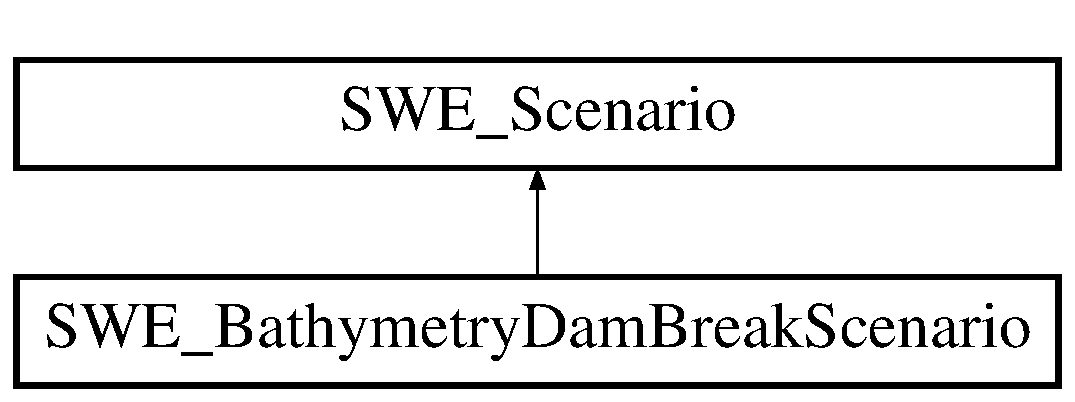
\includegraphics[height=2.000000cm]{classSWE__BathymetryDamBreakScenario}
\end{center}
\end{figure}
\subsection*{Public Member Functions}
\begin{DoxyCompactItemize}
\item 
\hypertarget{classSWE__BathymetryDamBreakScenario_abbc8b6d317163f21d2e9d46f67a6465f}{float {\bfseries get\-Bathymetry} (float x, float y)}\label{classSWE__BathymetryDamBreakScenario_abbc8b6d317163f21d2e9d46f67a6465f}

\item 
\hypertarget{classSWE__BathymetryDamBreakScenario_a29a5d3d82ad7092504b79a263c766feb}{virtual float {\bfseries end\-Simulation} ()}\label{classSWE__BathymetryDamBreakScenario_a29a5d3d82ad7092504b79a263c766feb}

\item 
\hypertarget{classSWE__BathymetryDamBreakScenario_ac7a07d56d659238c0dc099c6251e265b}{virtual \hyperlink{SWE__Scenario_8hh_af75d5dd7322fa39ed0af4e7839e600f8}{Boundary\-Type} {\bfseries get\-Boundary\-Type} (\hyperlink{SWE__Scenario_8hh_aa5e01e3f7df312f7b9b0d02521141fcc}{Boundary\-Edge} edge)}\label{classSWE__BathymetryDamBreakScenario_ac7a07d56d659238c0dc099c6251e265b}

\item 
float \hyperlink{classSWE__BathymetryDamBreakScenario_aa861ba2d4d7e71509f78e1d4d4cb82c7}{get\-Boundary\-Pos} (\hyperlink{SWE__Scenario_8hh_aa5e01e3f7df312f7b9b0d02521141fcc}{Boundary\-Edge} i\-\_\-edge)
\item 
float \hyperlink{classSWE__BathymetryDamBreakScenario_aa903538480526b092fff75160d7e225c}{get\-Water\-Height} (float i\-\_\-position\-X, float i\-\_\-position\-Y)
\end{DoxyCompactItemize}
\subsection*{Additional Inherited Members}


\subsection{Detailed Description}
Scenario \char`\"{}\-Bathymetry Dam Break\char`\"{}\-: uniform water depth, but elevated bathymetry in the centre of the domain 

\subsection{Member Function Documentation}
\hypertarget{classSWE__BathymetryDamBreakScenario_aa861ba2d4d7e71509f78e1d4d4cb82c7}{\index{S\-W\-E\-\_\-\-Bathymetry\-Dam\-Break\-Scenario@{S\-W\-E\-\_\-\-Bathymetry\-Dam\-Break\-Scenario}!get\-Boundary\-Pos@{get\-Boundary\-Pos}}
\index{get\-Boundary\-Pos@{get\-Boundary\-Pos}!SWE_BathymetryDamBreakScenario@{S\-W\-E\-\_\-\-Bathymetry\-Dam\-Break\-Scenario}}
\subsubsection[{get\-Boundary\-Pos}]{\setlength{\rightskip}{0pt plus 5cm}float S\-W\-E\-\_\-\-Bathymetry\-Dam\-Break\-Scenario\-::get\-Boundary\-Pos (
\begin{DoxyParamCaption}
\item[{{\bf Boundary\-Edge}}]{i\-\_\-edge}
\end{DoxyParamCaption}
)\hspace{0.3cm}{\ttfamily [inline]}, {\ttfamily [virtual]}}}\label{classSWE__BathymetryDamBreakScenario_aa861ba2d4d7e71509f78e1d4d4cb82c7}
Get the boundary positions


\begin{DoxyParams}{Parameters}
{\em i\-\_\-edge} & which edge \\
\hline
\end{DoxyParams}
\begin{DoxyReturn}{Returns}
value in the corresponding dimension 
\end{DoxyReturn}


Reimplemented from \hyperlink{classSWE__Scenario}{S\-W\-E\-\_\-\-Scenario}.

\hypertarget{classSWE__BathymetryDamBreakScenario_aa903538480526b092fff75160d7e225c}{\index{S\-W\-E\-\_\-\-Bathymetry\-Dam\-Break\-Scenario@{S\-W\-E\-\_\-\-Bathymetry\-Dam\-Break\-Scenario}!get\-Water\-Height@{get\-Water\-Height}}
\index{get\-Water\-Height@{get\-Water\-Height}!SWE_BathymetryDamBreakScenario@{S\-W\-E\-\_\-\-Bathymetry\-Dam\-Break\-Scenario}}
\subsubsection[{get\-Water\-Height}]{\setlength{\rightskip}{0pt plus 5cm}float S\-W\-E\-\_\-\-Bathymetry\-Dam\-Break\-Scenario\-::get\-Water\-Height (
\begin{DoxyParamCaption}
\item[{float}]{i\-\_\-position\-X, }
\item[{float}]{i\-\_\-position\-Y}
\end{DoxyParamCaption}
)\hspace{0.3cm}{\ttfamily [inline]}, {\ttfamily [virtual]}}}\label{classSWE__BathymetryDamBreakScenario_aa903538480526b092fff75160d7e225c}
Get the water height at a specific location.


\begin{DoxyParams}{Parameters}
{\em i\-\_\-position\-X} & position relative to the origin of the bathymetry grid in x-\/direction \\
\hline
{\em i\-\_\-position\-Y} & position relative to the origin of the bathymetry grid in y-\/direction \\
\hline
\end{DoxyParams}
\begin{DoxyReturn}{Returns}
water height (before the initial displacement) 
\end{DoxyReturn}


Reimplemented from \hyperlink{classSWE__Scenario}{S\-W\-E\-\_\-\-Scenario}.



The documentation for this class was generated from the following file\-:\begin{DoxyCompactItemize}
\item 
/home/sascha/\-Dokumente/\-Projects/\-Tsun\-Sim/\-S\-W\-E/src/scenarios/\hyperlink{SWE__simple__scenarios_8hh}{S\-W\-E\-\_\-simple\-\_\-scenarios.\-hh}\end{DoxyCompactItemize}

\hypertarget{classSWE__BathymetryDamBreakVisInfo}{\section{S\-W\-E\-\_\-\-Bathymetry\-Dam\-Break\-Vis\-Info Class Reference}
\label{classSWE__BathymetryDamBreakVisInfo}\index{S\-W\-E\-\_\-\-Bathymetry\-Dam\-Break\-Vis\-Info@{S\-W\-E\-\_\-\-Bathymetry\-Dam\-Break\-Vis\-Info}}
}


{\ttfamily \#include $<$S\-W\-E\-\_\-simple\-\_\-scenarios\-\_\-vis.\-hh$>$}

Inheritance diagram for S\-W\-E\-\_\-\-Bathymetry\-Dam\-Break\-Vis\-Info\-:\begin{figure}[H]
\begin{center}
\leavevmode
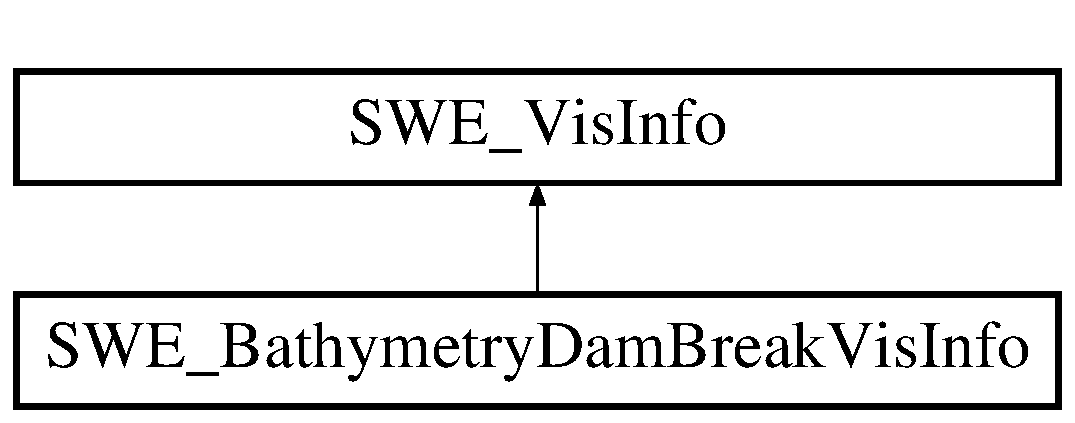
\includegraphics[height=2.000000cm]{classSWE__BathymetryDamBreakVisInfo}
\end{center}
\end{figure}
\subsection*{Public Member Functions}
\begin{DoxyCompactItemize}
\item 
float \hyperlink{classSWE__BathymetryDamBreakVisInfo_aaecf007665b780a6066485ea0d2d2695}{bathy\-Vertical\-Offset} ()
\end{DoxyCompactItemize}


\subsection{Detailed Description}
Vis\-Info \char`\"{}\-Bathymetry Dam Break\char`\"{}\-: uniform water depth, but elevated bathymetry in the center of the domain Set bathymetry offset hence it is visible in the screen 

\subsection{Member Function Documentation}
\hypertarget{classSWE__BathymetryDamBreakVisInfo_aaecf007665b780a6066485ea0d2d2695}{\index{S\-W\-E\-\_\-\-Bathymetry\-Dam\-Break\-Vis\-Info@{S\-W\-E\-\_\-\-Bathymetry\-Dam\-Break\-Vis\-Info}!bathy\-Vertical\-Offset@{bathy\-Vertical\-Offset}}
\index{bathy\-Vertical\-Offset@{bathy\-Vertical\-Offset}!SWE_BathymetryDamBreakVisInfo@{S\-W\-E\-\_\-\-Bathymetry\-Dam\-Break\-Vis\-Info}}
\subsubsection[{bathy\-Vertical\-Offset}]{\setlength{\rightskip}{0pt plus 5cm}float S\-W\-E\-\_\-\-Bathymetry\-Dam\-Break\-Vis\-Info\-::bathy\-Vertical\-Offset (
\begin{DoxyParamCaption}
{}
\end{DoxyParamCaption}
)\hspace{0.3cm}{\ttfamily [inline]}, {\ttfamily [virtual]}}}\label{classSWE__BathymetryDamBreakVisInfo_aaecf007665b780a6066485ea0d2d2695}
\begin{DoxyReturn}{Returns}
The vertical offset for the bathymetry. Should be 0 for \char`\"{}real\char`\"{} scenarios (scenarios with dry areas) 
\end{DoxyReturn}


Reimplemented from \hyperlink{classSWE__VisInfo_a9c24e444c209f6f0c03a96950931e677}{S\-W\-E\-\_\-\-Vis\-Info}.



The documentation for this class was generated from the following file\-:\begin{DoxyCompactItemize}
\item 
src/scenarios/S\-W\-E\-\_\-simple\-\_\-scenarios\-\_\-vis.\-hh\end{DoxyCompactItemize}

\hypertarget{classSWE__Block}{\section{S\-W\-E\-\_\-\-Block Class Reference}
\label{classSWE__Block}\index{S\-W\-E\-\_\-\-Block@{S\-W\-E\-\_\-\-Block}}
}


{\ttfamily \#include $<$S\-W\-E\-\_\-\-Block.\-hh$>$}

Inheritance diagram for S\-W\-E\-\_\-\-Block\-:\begin{figure}[H]
\begin{center}
\leavevmode
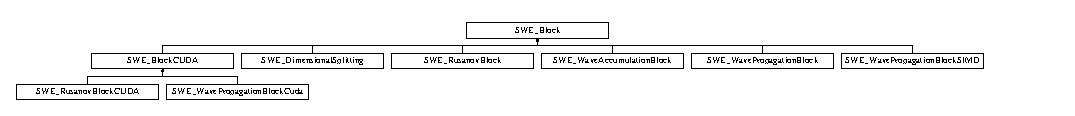
\includegraphics[height=1.111111cm]{classSWE__Block}
\end{center}
\end{figure}
\subsection*{Public Member Functions}
\begin{DoxyCompactItemize}
\item 
void \hyperlink{classSWE__Block_a46b715c584468a5daa975ec1eb1ab947}{init\-Scenario} (float \-\_\-offset\-X, float \-\_\-offset\-Y, \hyperlink{classSWE__Scenario}{S\-W\-E\-\_\-\-Scenario} \&i\-\_\-scenario, const bool i\-\_\-multiple\-Blocks=false)
\begin{DoxyCompactList}\small\item\em initialise unknowns to a specific scenario\-: \end{DoxyCompactList}\item 
void \hyperlink{classSWE__Block_a6481ce1c80a219fbefefdcbd13ed3688}{set\-Water\-Height} (float($\ast$\-\_\-h)(float, float))
\begin{DoxyCompactList}\small\item\em set the water height according to a given function \end{DoxyCompactList}\item 
void \hyperlink{classSWE__Block_a245332c325fd0ff6a7e9c2d3d9454970}{set\-Discharge} (float($\ast$\-\_\-u)(float, float), float($\ast$\-\_\-v)(float, float))
\begin{DoxyCompactList}\small\item\em set the momentum/discharge according to the provided functions \end{DoxyCompactList}\item 
void \hyperlink{classSWE__Block_af2ab34b138a14f2c295849f3b2acc5f3}{set\-Bathymetry} (float \-\_\-b)
\begin{DoxyCompactList}\small\item\em set the bathymetry to a uniform value \end{DoxyCompactList}\item 
void \hyperlink{classSWE__Block_ad4214fcfd102a4c167d274ad87d9dd90}{set\-Bathymetry} (float($\ast$\-\_\-b)(float, float))
\begin{DoxyCompactList}\small\item\em set the bathymetry according to a given function \end{DoxyCompactList}\item 
void \hyperlink{classSWE__Block_ab2e750bb5e8a952cd9f771054cb4e7b0}{set\-Bathymetry} (float $\ast$\-\_\-b)
\begin{DoxyCompactList}\small\item\em set the whole bathymetry matrix \end{DoxyCompactList}\item 
void \hyperlink{classSWE__Block_a54d2adb939d59e064edd7316faae445f}{set\-Bathymetry} (int i\-\_\-x, int i\-\_\-y, float i\-\_\-b)
\begin{DoxyCompactList}\small\item\em set one single cell's bathymetry value \end{DoxyCompactList}\item 
const \hyperlink{classFloat2D}{Float2\-D} \& \hyperlink{classSWE__Block_ab1aea4294403c194180c3dc107339fd7}{get\-Water\-Height} ()
\begin{DoxyCompactList}\small\item\em provides read access to the water height array \end{DoxyCompactList}\item 
const \hyperlink{classFloat2D}{Float2\-D} \& \hyperlink{classSWE__Block_ae5e766626a1e3fee89625610e2c67f1f}{get\-Discharge\-\_\-hu} ()
\begin{DoxyCompactList}\small\item\em provides read access to the momentum/discharge array (x-\/component) \end{DoxyCompactList}\item 
const \hyperlink{classFloat2D}{Float2\-D} \& \hyperlink{classSWE__Block_aece9e8dc3f9b8ab27420e537c76daf7c}{get\-Discharge\-\_\-hv} ()
\begin{DoxyCompactList}\small\item\em provides read access to the momentum/discharge array (y-\/component) \end{DoxyCompactList}\item 
const \hyperlink{classFloat2D}{Float2\-D} \& \hyperlink{classSWE__Block_a98e2c99a335d11d09a1489d6873b5615}{get\-Bathymetry} ()
\begin{DoxyCompactList}\small\item\em provides read access to the bathymetry data \end{DoxyCompactList}\item 
void \hyperlink{classSWE__Block_aa220b93e43b10f56c72a44d7363645c1}{set\-Boundary\-Type} (\hyperlink{SWE__Scenario_8hh_aa5e01e3f7df312f7b9b0d02521141fcc}{Boundary\-Edge} edge, \hyperlink{SWE__Scenario_8hh_af75d5dd7322fa39ed0af4e7839e600f8}{Boundary\-Type} boundtype, const \hyperlink{structSWE__Block1D}{S\-W\-E\-\_\-\-Block1\-D} $\ast$inflow=N\-U\-L\-L)
\begin{DoxyCompactList}\small\item\em set type of boundary condition for the specified boundary \end{DoxyCompactList}\item 
virtual \hyperlink{structSWE__Block1D}{S\-W\-E\-\_\-\-Block1\-D} $\ast$ \hyperlink{classSWE__Block_a827ee5c61dc9c1b472ac8b4e1c19956a}{register\-Copy\-Layer} (\hyperlink{SWE__Scenario_8hh_aa5e01e3f7df312f7b9b0d02521141fcc}{Boundary\-Edge} edge)
\begin{DoxyCompactList}\small\item\em return a pointer to proxy class to access the copy layer \end{DoxyCompactList}\item 
virtual \hyperlink{structSWE__Block1D}{S\-W\-E\-\_\-\-Block1\-D} $\ast$ \hyperlink{classSWE__Block_a9a96c59444645e237d098803009158a3}{grab\-Ghost\-Layer} (\hyperlink{SWE__Scenario_8hh_aa5e01e3f7df312f7b9b0d02521141fcc}{Boundary\-Edge} edge)
\begin{DoxyCompactList}\small\item\em \char`\"{}grab\char`\"{} the ghost layer in order to set these values externally \end{DoxyCompactList}\item 
void \hyperlink{classSWE__Block_afd17334abee3145e27cc3c9b7b935da2}{set\-Ghost\-Layer} ()
\begin{DoxyCompactList}\small\item\em set values in ghost layers \end{DoxyCompactList}\item 
float \hyperlink{classSWE__Block_a74da1eb712e639e47b5b848081b2afad}{get\-Max\-Timestep} ()
\begin{DoxyCompactList}\small\item\em return maximum size of the time step to ensure stability of the method \end{DoxyCompactList}\item 
void \hyperlink{classSWE__Block_acf2ff6617cbc0d3d837f0e618039cfe2}{compute\-Max\-Timestep} (const float i\-\_\-dry\-Tol=0.\-1, const float i\-\_\-cfl\-Number=0.\-4)
\item 
virtual void \hyperlink{classSWE__Block_add6908e1ceb261a0a1f3ebc262cc5f11}{simulate\-Timestep} (float dt)
\begin{DoxyCompactList}\small\item\em execute a single time step (with fixed time step size) of the simulation \end{DoxyCompactList}\item 
virtual float \hyperlink{classSWE__Block_a69784e2be2d09035fb2af9d306768f07}{simulate} (float t\-Start, float t\-End)
\item 
virtual void \hyperlink{classSWE__Block_a94dcf2c6ae31731e4586e45628b0c00e}{compute\-Numerical\-Fluxes} ()=0
\begin{DoxyCompactList}\small\item\em compute the numerical fluxes for each edge of the Cartesian grid \end{DoxyCompactList}\item 
virtual void \hyperlink{classSWE__Block_ab2b4b659f23d5d45413dece8d2da3298}{update\-Unknowns} (float dt)=0
\begin{DoxyCompactList}\small\item\em compute the new values of the unknowns h, hu, and hv in all grid cells \end{DoxyCompactList}\item 
\hypertarget{classSWE__Block_aa27028fa4bc13bb2d9251b09e0fdfce6}{int \hyperlink{classSWE__Block_aa27028fa4bc13bb2d9251b09e0fdfce6}{get\-Nx} ()}\label{classSWE__Block_aa27028fa4bc13bb2d9251b09e0fdfce6}

\begin{DoxyCompactList}\small\item\em returns \hyperlink{classSWE__Block_a46ec0dc1157997bd255fb39924f1e2bb}{nx}, i.\-e. the grid size in x-\/direction \end{DoxyCompactList}\item 
\hypertarget{classSWE__Block_a4b65557b6f73ffb6454dad3dbf86e9ad}{int \hyperlink{classSWE__Block_a4b65557b6f73ffb6454dad3dbf86e9ad}{get\-Ny} ()}\label{classSWE__Block_a4b65557b6f73ffb6454dad3dbf86e9ad}

\begin{DoxyCompactList}\small\item\em returns \hyperlink{classSWE__Block_a3f139630d12423eb4bd7df3e45c7f5da}{ny}, i.\-e. the grid size in y-\/direction \end{DoxyCompactList}\item 
\hypertarget{classSWE__Block_a2d4b3b3a932f3895c4f013cd4bb319d3}{float \hyperlink{classSWE__Block_a2d4b3b3a932f3895c4f013cd4bb319d3}{get\-Dx} ()}\label{classSWE__Block_a2d4b3b3a932f3895c4f013cd4bb319d3}

\begin{DoxyCompactList}\small\item\em returns \hyperlink{classSWE__Block_af2262b1cce6834d939c5a2315dae49b1}{dx}, i.\-e. the cell size in x-\/direction \end{DoxyCompactList}\item 
\hypertarget{classSWE__Block_add4edc5f146a02c00187a81d93f00fb7}{float \hyperlink{classSWE__Block_add4edc5f146a02c00187a81d93f00fb7}{get\-Dy} ()}\label{classSWE__Block_add4edc5f146a02c00187a81d93f00fb7}

\begin{DoxyCompactList}\small\item\em returns \hyperlink{classSWE__Block_a9feb988748d792bca0ca0508e43bd87f}{dy}, i.\-e. the cell size in y-\/direction \end{DoxyCompactList}\item 
\hypertarget{classSWE__Block_a5f279d69697c335d5e9c9c4d3c54e3b8}{float \hyperlink{classSWE__Block_a5f279d69697c335d5e9c9c4d3c54e3b8}{get\-Offx} ()}\label{classSWE__Block_a5f279d69697c335d5e9c9c4d3c54e3b8}

\begin{DoxyCompactList}\small\item\em return \hyperlink{classSWE__Block_aa9e9b1fa797c133c4989e4c54f09b542}{offset\-X}, i.\-e. the x-\/origin of the coordinate system \end{DoxyCompactList}\item 
\hypertarget{classSWE__Block_a22364064412b824204dc8a79bf572893}{float \hyperlink{classSWE__Block_a22364064412b824204dc8a79bf572893}{get\-Offy} ()}\label{classSWE__Block_a22364064412b824204dc8a79bf572893}

\begin{DoxyCompactList}\small\item\em return \hyperlink{classSWE__Block_aa05241101a66f0f0548eba6dbbaa1bbb}{offset\-Y}, i.\-e. the y-\/origin of the coordinate system \end{DoxyCompactList}\end{DoxyCompactItemize}
\subsection*{Static Public Attributes}
\begin{DoxyCompactItemize}
\item 
\hypertarget{classSWE__Block_a073ca743ff4077a7e456906be704958f}{static const float \hyperlink{classSWE__Block_a073ca743ff4077a7e456906be704958f}{g} = 9.\-81f}\label{classSWE__Block_a073ca743ff4077a7e456906be704958f}

\begin{DoxyCompactList}\small\item\em static variable that holds the gravity constant (g = 9.\-81 m/s$^\wedge$2)\-: \end{DoxyCompactList}\end{DoxyCompactItemize}
\subsection*{Protected Member Functions}
\begin{DoxyCompactItemize}
\item 
\hyperlink{classSWE__Block_a114ed3bb6a8a2c482e5f94f768543b82}{S\-W\-E\-\_\-\-Block} (int l\-\_\-nx, int l\-\_\-ny, float l\-\_\-dx, float l\-\_\-dy)
\item 
virtual \hyperlink{classSWE__Block_a2ddff1c284663ba514985a3574def1b0}{$\sim$\-S\-W\-E\-\_\-\-Block} ()
\item 
void \hyperlink{classSWE__Block_a6beb68dacde9c8479647c25c6a5cbcf5}{set\-Boundary\-Bathymetry} ()
\item 
virtual void \hyperlink{classSWE__Block_ae914f9bf6d4ef8f974f9f005114985e7}{synch\-After\-Write} ()
\item 
virtual void \hyperlink{classSWE__Block_aa2924833e29a795d8c04fb79bfe794de}{synch\-Water\-Height\-After\-Write} ()
\item 
virtual void \hyperlink{classSWE__Block_a94c34030153178c9d94f3f14be174eaf}{synch\-Discharge\-After\-Write} ()
\item 
virtual void \hyperlink{classSWE__Block_a4bece8aa90f67e55c40b91aab900febb}{synch\-Bathymetry\-After\-Write} ()
\item 
virtual void \hyperlink{classSWE__Block_a4657993ebdb5f0132b077e63790d0b2b}{synch\-Ghost\-Layer\-After\-Write} ()
\item 
virtual void \hyperlink{classSWE__Block_a23d936cb9a4367092e5b2515f81fe819}{synch\-Before\-Read} ()
\item 
virtual void \hyperlink{classSWE__Block_a07c85681ab29106c3b164db969899ace}{synch\-Water\-Height\-Before\-Read} ()
\item 
virtual void \hyperlink{classSWE__Block_a3773dcb194212fb8cb40ab8465575aa1}{synch\-Discharge\-Before\-Read} ()
\item 
virtual void \hyperlink{classSWE__Block_a7c8258c6949518ca44f4e9ce89d33b09}{synch\-Bathymetry\-Before\-Read} ()
\item 
virtual void \hyperlink{classSWE__Block_a13c90d5a6596336013c41e73c8795f83}{synch\-Copy\-Layer\-Before\-Read} ()
\item 
virtual void \hyperlink{classSWE__Block_a379807f0bf932b40aeb42065633fce60}{set\-Boundary\-Conditions} ()
\begin{DoxyCompactList}\small\item\em set boundary conditions in ghost layers (set boundary conditions) \end{DoxyCompactList}\end{DoxyCompactItemize}
\subsection*{Protected Attributes}
\begin{DoxyCompactItemize}
\item 
\hypertarget{classSWE__Block_a46ec0dc1157997bd255fb39924f1e2bb}{int \hyperlink{classSWE__Block_a46ec0dc1157997bd255fb39924f1e2bb}{nx}}\label{classSWE__Block_a46ec0dc1157997bd255fb39924f1e2bb}

\begin{DoxyCompactList}\small\item\em size of Cartesian arrays in x-\/direction \end{DoxyCompactList}\item 
\hypertarget{classSWE__Block_a3f139630d12423eb4bd7df3e45c7f5da}{int \hyperlink{classSWE__Block_a3f139630d12423eb4bd7df3e45c7f5da}{ny}}\label{classSWE__Block_a3f139630d12423eb4bd7df3e45c7f5da}

\begin{DoxyCompactList}\small\item\em size of Cartesian arrays in y-\/direction \end{DoxyCompactList}\item 
\hypertarget{classSWE__Block_af2262b1cce6834d939c5a2315dae49b1}{float \hyperlink{classSWE__Block_af2262b1cce6834d939c5a2315dae49b1}{dx}}\label{classSWE__Block_af2262b1cce6834d939c5a2315dae49b1}

\begin{DoxyCompactList}\small\item\em mesh size of the Cartesian grid in x-\/direction \end{DoxyCompactList}\item 
\hypertarget{classSWE__Block_a9feb988748d792bca0ca0508e43bd87f}{float \hyperlink{classSWE__Block_a9feb988748d792bca0ca0508e43bd87f}{dy}}\label{classSWE__Block_a9feb988748d792bca0ca0508e43bd87f}

\begin{DoxyCompactList}\small\item\em mesh size of the Cartesian grid in y-\/direction \end{DoxyCompactList}\item 
\hypertarget{classSWE__Block_a64a0f8f437f38b5f3b8ec5b4abdb864e}{\hyperlink{classFloat2D}{Float2\-D} \hyperlink{classSWE__Block_a64a0f8f437f38b5f3b8ec5b4abdb864e}{h}}\label{classSWE__Block_a64a0f8f437f38b5f3b8ec5b4abdb864e}

\begin{DoxyCompactList}\small\item\em array that holds the water height for each element \end{DoxyCompactList}\item 
\hypertarget{classSWE__Block_aec2c1278fdb23f083216d8d397f26060}{\hyperlink{classFloat2D}{Float2\-D} \hyperlink{classSWE__Block_aec2c1278fdb23f083216d8d397f26060}{hu}}\label{classSWE__Block_aec2c1278fdb23f083216d8d397f26060}

\begin{DoxyCompactList}\small\item\em array that holds the x-\/component of the momentum for each element (water height h multiplied by velocity in x-\/direction) \end{DoxyCompactList}\item 
\hypertarget{classSWE__Block_a0897aa3c2d78749f209c95e08196d831}{\hyperlink{classFloat2D}{Float2\-D} \hyperlink{classSWE__Block_a0897aa3c2d78749f209c95e08196d831}{hv}}\label{classSWE__Block_a0897aa3c2d78749f209c95e08196d831}

\begin{DoxyCompactList}\small\item\em array that holds the y-\/component of the momentum for each element (water height h multiplied by velocity in y-\/direction) \end{DoxyCompactList}\item 
\hypertarget{classSWE__Block_af7487209129f40b26ea171762754a261}{\hyperlink{classFloat2D}{Float2\-D} \hyperlink{classSWE__Block_af7487209129f40b26ea171762754a261}{b}}\label{classSWE__Block_af7487209129f40b26ea171762754a261}

\begin{DoxyCompactList}\small\item\em array that holds the bathymetry data (sea floor elevation) for each element \end{DoxyCompactList}\item 
\hypertarget{classSWE__Block_a0e56d0cad169abd4f5de95d9f96c7a73}{\hyperlink{SWE__Scenario_8hh_af75d5dd7322fa39ed0af4e7839e600f8}{Boundary\-Type} \hyperlink{classSWE__Block_a0e56d0cad169abd4f5de95d9f96c7a73}{boundary} \mbox{[}4\mbox{]}}\label{classSWE__Block_a0e56d0cad169abd4f5de95d9f96c7a73}

\begin{DoxyCompactList}\small\item\em type of boundary conditions at L\-E\-F\-T, R\-I\-G\-H\-T, T\-O\-P, and B\-O\-T\-T\-O\-M boundary \end{DoxyCompactList}\item 
\hypertarget{classSWE__Block_a5ea4ea4815af9eb66c51de9ad9b8d148}{const \hyperlink{structSWE__Block1D}{S\-W\-E\-\_\-\-Block1\-D} $\ast$ \hyperlink{classSWE__Block_a5ea4ea4815af9eb66c51de9ad9b8d148}{neighbour} \mbox{[}4\mbox{]}}\label{classSWE__Block_a5ea4ea4815af9eb66c51de9ad9b8d148}

\begin{DoxyCompactList}\small\item\em for C\-O\-N\-N\-E\-C\-T boundaries\-: pointer to connected neighbour block \end{DoxyCompactList}\item 
float \hyperlink{classSWE__Block_a05cbc9b40e0483bf73dbc2bdeae7dee3}{max\-Timestep}
\begin{DoxyCompactList}\small\item\em maximum time step allowed to ensure stability of the method \end{DoxyCompactList}\item 
\hypertarget{classSWE__Block_aa9e9b1fa797c133c4989e4c54f09b542}{float \hyperlink{classSWE__Block_aa9e9b1fa797c133c4989e4c54f09b542}{offset\-X}}\label{classSWE__Block_aa9e9b1fa797c133c4989e4c54f09b542}

\begin{DoxyCompactList}\small\item\em x-\/coordinate of the origin (left-\/bottom corner) of the Cartesian grid \end{DoxyCompactList}\item 
\hypertarget{classSWE__Block_aa05241101a66f0f0548eba6dbbaa1bbb}{float \hyperlink{classSWE__Block_aa05241101a66f0f0548eba6dbbaa1bbb}{offset\-Y}}\label{classSWE__Block_aa05241101a66f0f0548eba6dbbaa1bbb}

\begin{DoxyCompactList}\small\item\em y-\/coordinate of the origin (left-\/bottom corner) of the Cartesian grid \end{DoxyCompactList}\end{DoxyCompactItemize}


\subsection{Detailed Description}
\hyperlink{classSWE__Block}{S\-W\-E\-\_\-\-Block} is the main data structure to compute our shallow water model on a single Cartesian grid block\-: \hyperlink{classSWE__Block}{S\-W\-E\-\_\-\-Block} is an abstract class (and interface) that should be extended by respective implementation classes.

\paragraph*{Cartesian Grid for Discretization\-:}

S\-W\-E\-\_\-\-Blocks uses a regular Cartesian grid of size \hyperlink{classSWE__Block_a46ec0dc1157997bd255fb39924f1e2bb}{nx} by \hyperlink{classSWE__Block_a3f139630d12423eb4bd7df3e45c7f5da}{ny}, where each grid cell carries three unknowns\-:
\begin{DoxyItemize}
\item the water level \hyperlink{classSWE__Block_a64a0f8f437f38b5f3b8ec5b4abdb864e}{h}
\item the momentum components \hyperlink{classSWE__Block_aec2c1278fdb23f083216d8d397f26060}{hu} and \hyperlink{classSWE__Block_a0897aa3c2d78749f209c95e08196d831}{hv} (in x-\/ and y-\/ direction, resp.)
\item the bathymetry \hyperlink{classSWE__Block_af7487209129f40b26ea171762754a261}{b}
\end{DoxyItemize}

Each of the components is stored as a 2\-D array, implemented as a \hyperlink{classFloat2D}{Float2\-D} object, and are defined on grid indices \mbox{[}0,..,\hyperlink{classSWE__Block_a46ec0dc1157997bd255fb39924f1e2bb}{nx}+1\mbox{]}$\ast$\mbox{[}0,..,\hyperlink{classSWE__Block_a3f139630d12423eb4bd7df3e45c7f5da}{ny}+1\mbox{]}. The computational domain is indexed with \mbox{[}1,..,\hyperlink{classSWE__Block_a46ec0dc1157997bd255fb39924f1e2bb}{nx}\mbox{]}$\ast$\mbox{[}1,..,\hyperlink{classSWE__Block_a3f139630d12423eb4bd7df3e45c7f5da}{ny}\mbox{]}.

The mesh sizes of the grid in x-\/ and y-\/direction are stored in static variables \hyperlink{classSWE__Block_af2262b1cce6834d939c5a2315dae49b1}{dx} and \hyperlink{classSWE__Block_a9feb988748d792bca0ca0508e43bd87f}{dy}. The position of the Cartesian grid in space is stored via the coordinates of the left-\/bottom corner of the grid, in the variables \hyperlink{classSWE__Block_aa9e9b1fa797c133c4989e4c54f09b542}{offset\-X} and \hyperlink{classSWE__Block_aa05241101a66f0f0548eba6dbbaa1bbb}{offset\-Y}.

\paragraph*{Ghost layers\-:}

To implement the behaviour of the fluid at boundaries and for using multiple block in serial and parallel settings, \hyperlink{classSWE__Block}{S\-W\-E\-\_\-\-Block} adds an additional layer of so-\/called ghost cells to the Cartesian grid, as illustrated in the following figure. Cells in the ghost layer have indices 0 or \hyperlink{classSWE__Block_a46ec0dc1157997bd255fb39924f1e2bb}{nx}+1 / \hyperlink{classSWE__Block_a3f139630d12423eb4bd7df3e45c7f5da}{ny}+1.



\paragraph*{Memory Model\-:}

The variables \hyperlink{classSWE__Block_a64a0f8f437f38b5f3b8ec5b4abdb864e}{h}, \hyperlink{classSWE__Block_aec2c1278fdb23f083216d8d397f26060}{hu}, \hyperlink{classSWE__Block_a0897aa3c2d78749f209c95e08196d831}{hv} for water height and momentum will typically be updated by classes derived from \hyperlink{classSWE__Block}{S\-W\-E\-\_\-\-Block}. However, it is not assumed that such and updated will be performed in every time step. Instead, subclasses are welcome to update \hyperlink{classSWE__Block_a64a0f8f437f38b5f3b8ec5b4abdb864e}{h}, \hyperlink{classSWE__Block_aec2c1278fdb23f083216d8d397f26060}{hu}, and \hyperlink{classSWE__Block_a0897aa3c2d78749f209c95e08196d831}{hv} in a lazy fashion, and keep data in faster memory (incl. local memory of acceleration hardware, such as G\-P\-G\-P\-Us), instead.

It is assumed that the bathymetry data \hyperlink{classSWE__Block_af7487209129f40b26ea171762754a261}{b} is not changed during the algorithm (up to the exceptions mentioned in the following).

To force a synchronization of the respective data structures, the following methods are provided as part of \hyperlink{classSWE__Block}{S\-W\-E\-\_\-\-Block}\-:
\begin{DoxyItemize}
\item \hyperlink{classSWE__Block_ae914f9bf6d4ef8f974f9f005114985e7}{synch\-After\-Write()} to synchronize \hyperlink{classSWE__Block_a64a0f8f437f38b5f3b8ec5b4abdb864e}{h}, \hyperlink{classSWE__Block_aec2c1278fdb23f083216d8d397f26060}{hu}, \hyperlink{classSWE__Block_a0897aa3c2d78749f209c95e08196d831}{hv}, and \hyperlink{classSWE__Block_af7487209129f40b26ea171762754a261}{b} after an external update (reading a file, e.\-g.);
\item \hyperlink{classSWE__Block_aa2924833e29a795d8c04fb79bfe794de}{synch\-Water\-Height\-After\-Write()}, \hyperlink{classSWE__Block_a94c34030153178c9d94f3f14be174eaf}{synch\-Discharge\-After\-Write()}, \hyperlink{classSWE__Block_a4bece8aa90f67e55c40b91aab900febb}{synch\-Bathymetry\-After\-Write()}\-: to synchronize only \hyperlink{classSWE__Block_a64a0f8f437f38b5f3b8ec5b4abdb864e}{h} or momentum (\hyperlink{classSWE__Block_aec2c1278fdb23f083216d8d397f26060}{hu} and \hyperlink{classSWE__Block_a0897aa3c2d78749f209c95e08196d831}{hv}) or bathymetry \hyperlink{classSWE__Block_af7487209129f40b26ea171762754a261}{b};
\item \hyperlink{classSWE__Block_a4657993ebdb5f0132b077e63790d0b2b}{synch\-Ghost\-Layer\-After\-Write()} to synchronize only the ghost layers
\item \hyperlink{classSWE__Block_a23d936cb9a4367092e5b2515f81fe819}{synch\-Before\-Read()} to synchronize \hyperlink{classSWE__Block_a64a0f8f437f38b5f3b8ec5b4abdb864e}{h}, \hyperlink{classSWE__Block_aec2c1278fdb23f083216d8d397f26060}{hu}, \hyperlink{classSWE__Block_a0897aa3c2d78749f209c95e08196d831}{hv}, and \hyperlink{classSWE__Block_af7487209129f40b26ea171762754a261}{b} before an output of the variables (writing a visualization file, e.\-g.)
\item \hyperlink{classSWE__Block_a07c85681ab29106c3b164db969899ace}{synch\-Water\-Height\-Before\-Read()}, \hyperlink{classSWE__Block_a3773dcb194212fb8cb40ab8465575aa1}{synch\-Discharge\-Before\-Read()}, \hyperlink{classSWE__Block_a7c8258c6949518ca44f4e9ce89d33b09}{synch\-Bathymetry\-Before\-Read()}\-: as \hyperlink{classSWE__Block_a23d936cb9a4367092e5b2515f81fe819}{synch\-Before\-Read()}, but only for the specified variables
\item \hyperlink{classSWE__Block_a13c90d5a6596336013c41e73c8795f83}{synch\-Copy\-Layer\-Before\-Read()}\-: synchronizes the copy layer only (i.\-e., a layer that is to be replicated in a neighbouring \hyperlink{classSWE__Block}{S\-W\-E\-\_\-\-Block}.
\end{DoxyItemize}

\paragraph*{Derived Classes}

As \hyperlink{classSWE__Block}{S\-W\-E\-\_\-\-Block} just provides an abstract base class together with the most important data structures, the implementation of concrete models is the job of respective derived classes (see the class diagram at the top of this page). Similar, parallel implementations that are based on a specific parallel programming model (such as Open\-M\-P) or parallel architecture (such as G\-P\-U/\-C\-U\-D\-A) should form subclasses of their own. Please refer to the documentation of these classes for more details on the model and on the parallelisation approach. 

\subsection{Constructor \& Destructor Documentation}
\hypertarget{classSWE__Block_a114ed3bb6a8a2c482e5f94f768543b82}{\index{S\-W\-E\-\_\-\-Block@{S\-W\-E\-\_\-\-Block}!S\-W\-E\-\_\-\-Block@{S\-W\-E\-\_\-\-Block}}
\index{S\-W\-E\-\_\-\-Block@{S\-W\-E\-\_\-\-Block}!SWE_Block@{S\-W\-E\-\_\-\-Block}}
\subsubsection[{S\-W\-E\-\_\-\-Block}]{\setlength{\rightskip}{0pt plus 5cm}S\-W\-E\-\_\-\-Block\-::\-S\-W\-E\-\_\-\-Block (
\begin{DoxyParamCaption}
\item[{int}]{l\-\_\-nx, }
\item[{int}]{l\-\_\-ny, }
\item[{float}]{l\-\_\-dx, }
\item[{float}]{l\-\_\-dy}
\end{DoxyParamCaption}
)\hspace{0.3cm}{\ttfamily [protected]}}}\label{classSWE__Block_a114ed3bb6a8a2c482e5f94f768543b82}
Constructor\-: allocate variables for simulation

unknowns h (water height), hu,hv (discharge in x-\/ and y-\/direction), and b (bathymetry) are defined on grid indices \mbox{[}0,..,nx+1\mbox{]}$\ast$\mbox{[}0,..,ny+1\mbox{]} -\/$>$ computational domain is \mbox{[}1,..,nx\mbox{]}$\ast$\mbox{[}1,..,ny\mbox{]} -\/$>$ plus ghost cell layer

The constructor is protected\-: no instances of \hyperlink{classSWE__Block}{S\-W\-E\-\_\-\-Block} can be generated. \hypertarget{classSWE__Block_a2ddff1c284663ba514985a3574def1b0}{\index{S\-W\-E\-\_\-\-Block@{S\-W\-E\-\_\-\-Block}!$\sim$\-S\-W\-E\-\_\-\-Block@{$\sim$\-S\-W\-E\-\_\-\-Block}}
\index{$\sim$\-S\-W\-E\-\_\-\-Block@{$\sim$\-S\-W\-E\-\_\-\-Block}!SWE_Block@{S\-W\-E\-\_\-\-Block}}
\subsubsection[{$\sim$\-S\-W\-E\-\_\-\-Block}]{\setlength{\rightskip}{0pt plus 5cm}S\-W\-E\-\_\-\-Block\-::$\sim$\-S\-W\-E\-\_\-\-Block (
\begin{DoxyParamCaption}
{}
\end{DoxyParamCaption}
)\hspace{0.3cm}{\ttfamily [protected]}, {\ttfamily [virtual]}}}\label{classSWE__Block_a2ddff1c284663ba514985a3574def1b0}
Destructor\-: de-\/allocate all variables 

\subsection{Member Function Documentation}
\hypertarget{classSWE__Block_acf2ff6617cbc0d3d837f0e618039cfe2}{\index{S\-W\-E\-\_\-\-Block@{S\-W\-E\-\_\-\-Block}!compute\-Max\-Timestep@{compute\-Max\-Timestep}}
\index{compute\-Max\-Timestep@{compute\-Max\-Timestep}!SWE_Block@{S\-W\-E\-\_\-\-Block}}
\subsubsection[{compute\-Max\-Timestep}]{\setlength{\rightskip}{0pt plus 5cm}void S\-W\-E\-\_\-\-Block\-::compute\-Max\-Timestep (
\begin{DoxyParamCaption}
\item[{const float}]{i\-\_\-dry\-Tol = {\ttfamily 0.1}, }
\item[{const float}]{i\-\_\-cfl\-Number = {\ttfamily 0.4}}
\end{DoxyParamCaption}
)}}\label{classSWE__Block_acf2ff6617cbc0d3d837f0e618039cfe2}
Compute the largest allowed time step for the current grid block (reference implementation) depending on the current values of variables h, hu, and hv, and store this time step size in member variable max\-Timestep.


\begin{DoxyParams}{Parameters}
{\em i\-\_\-dry\-Tol} & dry tolerance (dry cells do not affect the time step). \\
\hline
{\em i\-\_\-cfl\-Number} & C\-F\-L number of the used method. \\
\hline
\end{DoxyParams}
\hypertarget{classSWE__Block_a94dcf2c6ae31731e4586e45628b0c00e}{\index{S\-W\-E\-\_\-\-Block@{S\-W\-E\-\_\-\-Block}!compute\-Numerical\-Fluxes@{compute\-Numerical\-Fluxes}}
\index{compute\-Numerical\-Fluxes@{compute\-Numerical\-Fluxes}!SWE_Block@{S\-W\-E\-\_\-\-Block}}
\subsubsection[{compute\-Numerical\-Fluxes}]{\setlength{\rightskip}{0pt plus 5cm}virtual void S\-W\-E\-\_\-\-Block\-::compute\-Numerical\-Fluxes (
\begin{DoxyParamCaption}
{}
\end{DoxyParamCaption}
)\hspace{0.3cm}{\ttfamily [pure virtual]}}}\label{classSWE__Block_a94dcf2c6ae31731e4586e45628b0c00e}


compute the numerical fluxes for each edge of the Cartesian grid 

The computation of fluxes strongly depends on the chosen numerical method. Hence, this purely virtual function has to be implemented in the respective derived classes. 

Implemented in \hyperlink{classSWE__WavePropagationBlockSIMD_a4aa15050ec1db113f54fff06539a900f}{S\-W\-E\-\_\-\-Wave\-Propagation\-Block\-S\-I\-M\-D}, \hyperlink{classSWE__DimensionalSplitting_a84759f8fbbbfe1e46613375515826f0f}{S\-W\-E\-\_\-\-Dimensional\-Splitting}, \hyperlink{classSWE__WavePropagationBlock_a5f6335a38fb3cf38623326959f06baf4}{S\-W\-E\-\_\-\-Wave\-Propagation\-Block}, \hyperlink{classSWE__WavePropagationBlockCuda_a8a89bf61b9fc4433652f400ca8e564ed}{S\-W\-E\-\_\-\-Wave\-Propagation\-Block\-Cuda}, \hyperlink{classSWE__WaveAccumulationBlock_acac0b73f22b256bc91a58ff8d0831e5d}{S\-W\-E\-\_\-\-Wave\-Accumulation\-Block}, \hyperlink{classSWE__RusanovBlock_a78cdefa510cd2d88ca4e213f75b9b10b}{S\-W\-E\-\_\-\-Rusanov\-Block}, and \hyperlink{classSWE__RusanovBlockCUDA_a85ec49606ab69ded8cd6f39aa4be1505}{S\-W\-E\-\_\-\-Rusanov\-Block\-C\-U\-D\-A}.

\hypertarget{classSWE__Block_a98e2c99a335d11d09a1489d6873b5615}{\index{S\-W\-E\-\_\-\-Block@{S\-W\-E\-\_\-\-Block}!get\-Bathymetry@{get\-Bathymetry}}
\index{get\-Bathymetry@{get\-Bathymetry}!SWE_Block@{S\-W\-E\-\_\-\-Block}}
\subsubsection[{get\-Bathymetry}]{\setlength{\rightskip}{0pt plus 5cm}const {\bf Float2\-D} \& S\-W\-E\-\_\-\-Block\-::get\-Bathymetry (
\begin{DoxyParamCaption}
{}
\end{DoxyParamCaption}
)}}\label{classSWE__Block_a98e2c99a335d11d09a1489d6873b5615}


provides read access to the bathymetry data 

return reference to bathymetry unknown b \hypertarget{classSWE__Block_ae5e766626a1e3fee89625610e2c67f1f}{\index{S\-W\-E\-\_\-\-Block@{S\-W\-E\-\_\-\-Block}!get\-Discharge\-\_\-hu@{get\-Discharge\-\_\-hu}}
\index{get\-Discharge\-\_\-hu@{get\-Discharge\-\_\-hu}!SWE_Block@{S\-W\-E\-\_\-\-Block}}
\subsubsection[{get\-Discharge\-\_\-hu}]{\setlength{\rightskip}{0pt plus 5cm}const {\bf Float2\-D} \& S\-W\-E\-\_\-\-Block\-::get\-Discharge\-\_\-hu (
\begin{DoxyParamCaption}
{}
\end{DoxyParamCaption}
)}}\label{classSWE__Block_ae5e766626a1e3fee89625610e2c67f1f}


provides read access to the momentum/discharge array (x-\/component) 

return reference to discharge unknown hu \hypertarget{classSWE__Block_aece9e8dc3f9b8ab27420e537c76daf7c}{\index{S\-W\-E\-\_\-\-Block@{S\-W\-E\-\_\-\-Block}!get\-Discharge\-\_\-hv@{get\-Discharge\-\_\-hv}}
\index{get\-Discharge\-\_\-hv@{get\-Discharge\-\_\-hv}!SWE_Block@{S\-W\-E\-\_\-\-Block}}
\subsubsection[{get\-Discharge\-\_\-hv}]{\setlength{\rightskip}{0pt plus 5cm}const {\bf Float2\-D} \& S\-W\-E\-\_\-\-Block\-::get\-Discharge\-\_\-hv (
\begin{DoxyParamCaption}
{}
\end{DoxyParamCaption}
)}}\label{classSWE__Block_aece9e8dc3f9b8ab27420e537c76daf7c}


provides read access to the momentum/discharge array (y-\/component) 

return reference to discharge unknown hv \hypertarget{classSWE__Block_a74da1eb712e639e47b5b848081b2afad}{\index{S\-W\-E\-\_\-\-Block@{S\-W\-E\-\_\-\-Block}!get\-Max\-Timestep@{get\-Max\-Timestep}}
\index{get\-Max\-Timestep@{get\-Max\-Timestep}!SWE_Block@{S\-W\-E\-\_\-\-Block}}
\subsubsection[{get\-Max\-Timestep}]{\setlength{\rightskip}{0pt plus 5cm}float S\-W\-E\-\_\-\-Block\-::get\-Max\-Timestep (
\begin{DoxyParamCaption}
{}
\end{DoxyParamCaption}
)\hspace{0.3cm}{\ttfamily [inline]}}}\label{classSWE__Block_a74da1eb712e639e47b5b848081b2afad}


return maximum size of the time step to ensure stability of the method 

\begin{DoxyReturn}{Returns}
current value of the member variable \hyperlink{classSWE__Block_a05cbc9b40e0483bf73dbc2bdeae7dee3}{max\-Timestep} 
\end{DoxyReturn}
\hypertarget{classSWE__Block_ab1aea4294403c194180c3dc107339fd7}{\index{S\-W\-E\-\_\-\-Block@{S\-W\-E\-\_\-\-Block}!get\-Water\-Height@{get\-Water\-Height}}
\index{get\-Water\-Height@{get\-Water\-Height}!SWE_Block@{S\-W\-E\-\_\-\-Block}}
\subsubsection[{get\-Water\-Height}]{\setlength{\rightskip}{0pt plus 5cm}const {\bf Float2\-D} \& S\-W\-E\-\_\-\-Block\-::get\-Water\-Height (
\begin{DoxyParamCaption}
{}
\end{DoxyParamCaption}
)}}\label{classSWE__Block_ab1aea4294403c194180c3dc107339fd7}


provides read access to the water height array 

return reference to water height unknown h \hypertarget{classSWE__Block_a9a96c59444645e237d098803009158a3}{\index{S\-W\-E\-\_\-\-Block@{S\-W\-E\-\_\-\-Block}!grab\-Ghost\-Layer@{grab\-Ghost\-Layer}}
\index{grab\-Ghost\-Layer@{grab\-Ghost\-Layer}!SWE_Block@{S\-W\-E\-\_\-\-Block}}
\subsubsection[{grab\-Ghost\-Layer}]{\setlength{\rightskip}{0pt plus 5cm}{\bf S\-W\-E\-\_\-\-Block1\-D} $\ast$ S\-W\-E\-\_\-\-Block\-::grab\-Ghost\-Layer (
\begin{DoxyParamCaption}
\item[{{\bf Boundary\-Edge}}]{edge}
\end{DoxyParamCaption}
)\hspace{0.3cm}{\ttfamily [virtual]}}}\label{classSWE__Block_a9a96c59444645e237d098803009158a3}


\char`\"{}grab\char`\"{} the ghost layer in order to set these values externally 

\char`\"{}grab\char`\"{} the ghost layer at the specific boundary in order to set boundary values in this ghost layer externally. The boundary conditions at the respective ghost layer is set to P\-A\-S\-S\-I\-V\-E, such that the grabbing program component is responsible to provide correct values in the ghost layer, for example by receiving data from a remote copy layer via M\-P\-I communication. 
\begin{DoxyParams}{Parameters}
{\em specified} & edge \\
\hline
\end{DoxyParams}
\begin{DoxyReturn}{Returns}
a \hyperlink{structSWE__Block1D}{S\-W\-E\-\_\-\-Block1\-D} object that contains row variables h, hu, and hv 
\end{DoxyReturn}


Reimplemented in \hyperlink{classSWE__BlockCUDA_ab8671269d89d544a333a0b8c0fa72f37}{S\-W\-E\-\_\-\-Block\-C\-U\-D\-A}.

\hypertarget{classSWE__Block_a46b715c584468a5daa975ec1eb1ab947}{\index{S\-W\-E\-\_\-\-Block@{S\-W\-E\-\_\-\-Block}!init\-Scenario@{init\-Scenario}}
\index{init\-Scenario@{init\-Scenario}!SWE_Block@{S\-W\-E\-\_\-\-Block}}
\subsubsection[{init\-Scenario}]{\setlength{\rightskip}{0pt plus 5cm}void S\-W\-E\-\_\-\-Block\-::init\-Scenario (
\begin{DoxyParamCaption}
\item[{float}]{\-\_\-offset\-X, }
\item[{float}]{\-\_\-offset\-Y, }
\item[{{\bf S\-W\-E\-\_\-\-Scenario} \&}]{i\-\_\-scenario, }
\item[{const bool}]{i\-\_\-multiple\-Blocks = {\ttfamily false}}
\end{DoxyParamCaption}
)}}\label{classSWE__Block_a46b715c584468a5daa975ec1eb1ab947}


initialise unknowns to a specific scenario\-: 

Initializes the unknowns and bathymetry in all grid cells according to the given \hyperlink{classSWE__Scenario}{S\-W\-E\-\_\-\-Scenario}.

In the case of multiple S\-W\-E\-\_\-\-Blocks at this point, it is not clear how the boundary conditions should be set. This is because an isolated \hyperlink{classSWE__Block}{S\-W\-E\-\_\-\-Block} doesn't have any in information about the grid. Therefore the calling routine, which has the information about multiple blocks, has to take care about setting the right boundary conditions.


\begin{DoxyParams}{Parameters}
{\em i\-\_\-scenario} & scenario, which is used during the setup. \\
\hline
{\em i\-\_\-multiple\-Blocks} & are the multiple S\-W\-E\-\_\-blocks? \\
\hline
\end{DoxyParams}
\hypertarget{classSWE__Block_a827ee5c61dc9c1b472ac8b4e1c19956a}{\index{S\-W\-E\-\_\-\-Block@{S\-W\-E\-\_\-\-Block}!register\-Copy\-Layer@{register\-Copy\-Layer}}
\index{register\-Copy\-Layer@{register\-Copy\-Layer}!SWE_Block@{S\-W\-E\-\_\-\-Block}}
\subsubsection[{register\-Copy\-Layer}]{\setlength{\rightskip}{0pt plus 5cm}{\bf S\-W\-E\-\_\-\-Block1\-D} $\ast$ S\-W\-E\-\_\-\-Block\-::register\-Copy\-Layer (
\begin{DoxyParamCaption}
\item[{{\bf Boundary\-Edge}}]{edge}
\end{DoxyParamCaption}
)\hspace{0.3cm}{\ttfamily [virtual]}}}\label{classSWE__Block_a827ee5c61dc9c1b472ac8b4e1c19956a}


return a pointer to proxy class to access the copy layer 

register the row or column layer next to a boundary as a \char`\"{}copy layer\char`\"{}, from which values will be copied into the ghost layer or a neighbour; \begin{DoxyReturn}{Returns}
a \hyperlink{structSWE__Block1D}{S\-W\-E\-\_\-\-Block1\-D} object that contains row variables h, hu, and hv 
\end{DoxyReturn}


Reimplemented in \hyperlink{classSWE__BlockCUDA_a22782766fc679ac14e9ba30a4efc1688}{S\-W\-E\-\_\-\-Block\-C\-U\-D\-A}.

\hypertarget{classSWE__Block_af2ab34b138a14f2c295849f3b2acc5f3}{\index{S\-W\-E\-\_\-\-Block@{S\-W\-E\-\_\-\-Block}!set\-Bathymetry@{set\-Bathymetry}}
\index{set\-Bathymetry@{set\-Bathymetry}!SWE_Block@{S\-W\-E\-\_\-\-Block}}
\subsubsection[{set\-Bathymetry}]{\setlength{\rightskip}{0pt plus 5cm}void S\-W\-E\-\_\-\-Block\-::set\-Bathymetry (
\begin{DoxyParamCaption}
\item[{float}]{\-\_\-b}
\end{DoxyParamCaption}
)}}\label{classSWE__Block_af2ab34b138a14f2c295849f3b2acc5f3}


set the bathymetry to a uniform value 

set Bathymetry b in all grid cells (incl. ghost/boundary layers) to a uniform value bathymetry source terms are re-\/computed \hypertarget{classSWE__Block_ad4214fcfd102a4c167d274ad87d9dd90}{\index{S\-W\-E\-\_\-\-Block@{S\-W\-E\-\_\-\-Block}!set\-Bathymetry@{set\-Bathymetry}}
\index{set\-Bathymetry@{set\-Bathymetry}!SWE_Block@{S\-W\-E\-\_\-\-Block}}
\subsubsection[{set\-Bathymetry}]{\setlength{\rightskip}{0pt plus 5cm}void S\-W\-E\-\_\-\-Block\-::set\-Bathymetry (
\begin{DoxyParamCaption}
\item[{float($\ast$)(float, float)}]{\-\_\-b}
\end{DoxyParamCaption}
)}}\label{classSWE__Block_ad4214fcfd102a4c167d274ad87d9dd90}


set the bathymetry according to a given function 

set Bathymetry b in all grid cells (incl. ghost/boundary layers) using the specified bathymetry function; bathymetry source terms are re-\/computed \hypertarget{classSWE__Block_ab2e750bb5e8a952cd9f771054cb4e7b0}{\index{S\-W\-E\-\_\-\-Block@{S\-W\-E\-\_\-\-Block}!set\-Bathymetry@{set\-Bathymetry}}
\index{set\-Bathymetry@{set\-Bathymetry}!SWE_Block@{S\-W\-E\-\_\-\-Block}}
\subsubsection[{set\-Bathymetry}]{\setlength{\rightskip}{0pt plus 5cm}void S\-W\-E\-\_\-\-Block\-::set\-Bathymetry (
\begin{DoxyParamCaption}
\item[{float $\ast$}]{\-\_\-b}
\end{DoxyParamCaption}
)}}\label{classSWE__Block_ab2e750bb5e8a952cd9f771054cb4e7b0}


set the whole bathymetry matrix 

Restores values for h, v, and u from file data 
\begin{DoxyParams}{Parameters}
{\em \-\_\-b} & array holding b-\/values in sequence \\
\hline
\end{DoxyParams}
\hypertarget{classSWE__Block_a54d2adb939d59e064edd7316faae445f}{\index{S\-W\-E\-\_\-\-Block@{S\-W\-E\-\_\-\-Block}!set\-Bathymetry@{set\-Bathymetry}}
\index{set\-Bathymetry@{set\-Bathymetry}!SWE_Block@{S\-W\-E\-\_\-\-Block}}
\subsubsection[{set\-Bathymetry}]{\setlength{\rightskip}{0pt plus 5cm}void S\-W\-E\-\_\-\-Block\-::set\-Bathymetry (
\begin{DoxyParamCaption}
\item[{int}]{i\-\_\-x, }
\item[{int}]{i\-\_\-y, }
\item[{float}]{i\-\_\-b}
\end{DoxyParamCaption}
)}}\label{classSWE__Block_a54d2adb939d59e064edd7316faae445f}


set one single cell's bathymetry value 

Sets the bathymetry value at one single cell

Assumption\-: User has no knowledge of ghost layer. if nx and ny were both zero, the only valid input for (i\-\_\-x, i\-\_\-y) would be (0, 0) 
\begin{DoxyParams}{Parameters}
{\em i\-\_\-b} & new bathymetry value \\
\hline
{\em i\-\_\-x} & x-\/coordinate of the cell \\
\hline
{\em i\-\_\-y} & y-\/coordinate of the cell \\
\hline
\end{DoxyParams}
\hypertarget{classSWE__Block_a6beb68dacde9c8479647c25c6a5cbcf5}{\index{S\-W\-E\-\_\-\-Block@{S\-W\-E\-\_\-\-Block}!set\-Boundary\-Bathymetry@{set\-Boundary\-Bathymetry}}
\index{set\-Boundary\-Bathymetry@{set\-Boundary\-Bathymetry}!SWE_Block@{S\-W\-E\-\_\-\-Block}}
\subsubsection[{set\-Boundary\-Bathymetry}]{\setlength{\rightskip}{0pt plus 5cm}void S\-W\-E\-\_\-\-Block\-::set\-Boundary\-Bathymetry (
\begin{DoxyParamCaption}
{}
\end{DoxyParamCaption}
)\hspace{0.3cm}{\ttfamily [protected]}}}\label{classSWE__Block_a6beb68dacde9c8479647c25c6a5cbcf5}
Sets the bathymetry on O\-U\-T\-F\-L\-O\-W or W\-A\-L\-L boundaries. Should be called very time a boundary is changed to a O\-U\-T\-F\-L\-O\-W or W\-A\-L\-L boundary {\bfseries or} the bathymetry changes. \hypertarget{classSWE__Block_a379807f0bf932b40aeb42065633fce60}{\index{S\-W\-E\-\_\-\-Block@{S\-W\-E\-\_\-\-Block}!set\-Boundary\-Conditions@{set\-Boundary\-Conditions}}
\index{set\-Boundary\-Conditions@{set\-Boundary\-Conditions}!SWE_Block@{S\-W\-E\-\_\-\-Block}}
\subsubsection[{set\-Boundary\-Conditions}]{\setlength{\rightskip}{0pt plus 5cm}void S\-W\-E\-\_\-\-Block\-::set\-Boundary\-Conditions (
\begin{DoxyParamCaption}
{}
\end{DoxyParamCaption}
)\hspace{0.3cm}{\ttfamily [protected]}, {\ttfamily [virtual]}}}\label{classSWE__Block_a379807f0bf932b40aeb42065633fce60}


set boundary conditions in ghost layers (set boundary conditions) 

set the values of all ghost cells depending on the specifed boundary conditions
\begin{DoxyItemize}
\item set boundary conditions for typs W\-A\-L\-L and O\-U\-T\-F\-L\-O\-W
\item derived classes need to transfer ghost layers 
\end{DoxyItemize}

Reimplemented in \hyperlink{classSWE__BlockCUDA_a7cf66067cb7f023aadbd910051d389c8}{S\-W\-E\-\_\-\-Block\-C\-U\-D\-A}.

\hypertarget{classSWE__Block_aa220b93e43b10f56c72a44d7363645c1}{\index{S\-W\-E\-\_\-\-Block@{S\-W\-E\-\_\-\-Block}!set\-Boundary\-Type@{set\-Boundary\-Type}}
\index{set\-Boundary\-Type@{set\-Boundary\-Type}!SWE_Block@{S\-W\-E\-\_\-\-Block}}
\subsubsection[{set\-Boundary\-Type}]{\setlength{\rightskip}{0pt plus 5cm}void S\-W\-E\-\_\-\-Block\-::set\-Boundary\-Type (
\begin{DoxyParamCaption}
\item[{{\bf Boundary\-Edge}}]{edge, }
\item[{{\bf Boundary\-Type}}]{boundtype, }
\item[{const {\bf S\-W\-E\-\_\-\-Block1\-D} $\ast$}]{i\-\_\-inflow = {\ttfamily NULL}}
\end{DoxyParamCaption}
)}}\label{classSWE__Block_aa220b93e43b10f56c72a44d7363645c1}


set type of boundary condition for the specified boundary 

Set the boundary type for specific block boundary.


\begin{DoxyParams}{Parameters}
{\em i\-\_\-edge} & location of the edge relative to the S\-W\-E\-\_\-block. \\
\hline
{\em i\-\_\-boundary\-Type} & type of the boundary condition. \\
\hline
{\em i\-\_\-inflow} & pointer to an \hyperlink{structSWE__Block1D}{S\-W\-E\-\_\-\-Block1\-D}, which specifies the inflow (should be N\-U\-L\-L for W\-A\-L\-L or O\-U\-T\-F\-L\-O\-W boundary) \\
\hline
\end{DoxyParams}
\hypertarget{classSWE__Block_a245332c325fd0ff6a7e9c2d3d9454970}{\index{S\-W\-E\-\_\-\-Block@{S\-W\-E\-\_\-\-Block}!set\-Discharge@{set\-Discharge}}
\index{set\-Discharge@{set\-Discharge}!SWE_Block@{S\-W\-E\-\_\-\-Block}}
\subsubsection[{set\-Discharge}]{\setlength{\rightskip}{0pt plus 5cm}void S\-W\-E\-\_\-\-Block\-::set\-Discharge (
\begin{DoxyParamCaption}
\item[{float($\ast$)(float, float)}]{\-\_\-u, }
\item[{float($\ast$)(float, float)}]{\-\_\-v}
\end{DoxyParamCaption}
)}}\label{classSWE__Block_a245332c325fd0ff6a7e9c2d3d9454970}


set the momentum/discharge according to the provided functions 

set discharge in all interior grid cells (i.\-e. except ghost layer) to values specified by parameter functions Note\-: unknowns hu and hv represent momentum, while parameters u and v are velocities! \hypertarget{classSWE__Block_afd17334abee3145e27cc3c9b7b935da2}{\index{S\-W\-E\-\_\-\-Block@{S\-W\-E\-\_\-\-Block}!set\-Ghost\-Layer@{set\-Ghost\-Layer}}
\index{set\-Ghost\-Layer@{set\-Ghost\-Layer}!SWE_Block@{S\-W\-E\-\_\-\-Block}}
\subsubsection[{set\-Ghost\-Layer}]{\setlength{\rightskip}{0pt plus 5cm}void S\-W\-E\-\_\-\-Block\-::set\-Ghost\-Layer (
\begin{DoxyParamCaption}
{}
\end{DoxyParamCaption}
)}}\label{classSWE__Block_afd17334abee3145e27cc3c9b7b935da2}


set values in ghost layers 

set the values of all ghost cells depending on the specifed boundary conditions; if the ghost layer replicates the variables of a remote \hyperlink{classSWE__Block}{S\-W\-E\-\_\-\-Block}, the values are copied \hypertarget{classSWE__Block_a6481ce1c80a219fbefefdcbd13ed3688}{\index{S\-W\-E\-\_\-\-Block@{S\-W\-E\-\_\-\-Block}!set\-Water\-Height@{set\-Water\-Height}}
\index{set\-Water\-Height@{set\-Water\-Height}!SWE_Block@{S\-W\-E\-\_\-\-Block}}
\subsubsection[{set\-Water\-Height}]{\setlength{\rightskip}{0pt plus 5cm}void S\-W\-E\-\_\-\-Block\-::set\-Water\-Height (
\begin{DoxyParamCaption}
\item[{float($\ast$)(float, float)}]{\-\_\-h}
\end{DoxyParamCaption}
)}}\label{classSWE__Block_a6481ce1c80a219fbefefdcbd13ed3688}


set the water height according to a given function 

set water height h in all interior grid cells (i.\-e. except ghost layer) to values specified by parameter function \-\_\-h \hypertarget{classSWE__Block_a69784e2be2d09035fb2af9d306768f07}{\index{S\-W\-E\-\_\-\-Block@{S\-W\-E\-\_\-\-Block}!simulate@{simulate}}
\index{simulate@{simulate}!SWE_Block@{S\-W\-E\-\_\-\-Block}}
\subsubsection[{simulate}]{\setlength{\rightskip}{0pt plus 5cm}float S\-W\-E\-\_\-\-Block\-::simulate (
\begin{DoxyParamCaption}
\item[{float}]{i\-\_\-t\-Start, }
\item[{float}]{i\-\_\-t\-End}
\end{DoxyParamCaption}
)\hspace{0.3cm}{\ttfamily [virtual]}}}\label{classSWE__Block_a69784e2be2d09035fb2af9d306768f07}
perform the simulation starting with simulation time t\-Start, until simulation time t\-End is reached

simulate implements the main simulation loop between two checkpoints; Note\-: this implementation can only be used, if you only use a single \hyperlink{classSWE__Block}{S\-W\-E\-\_\-\-Block} and only apply simple boundary conditions! In particular, \hyperlink{classSWE__Block_a69784e2be2d09035fb2af9d306768f07}{S\-W\-E\-\_\-\-Block\-::simulate} can not trigger calls to exchange values of copy and ghost layers between blocks! 
\begin{DoxyParams}{Parameters}
{\em t\-Start} & time where the simulation is started \\
\hline
{\em t\-End} & time of the next checkpoint \\
\hline
\end{DoxyParams}
\begin{DoxyReturn}{Returns}
actual end time reached 
\end{DoxyReturn}


Reimplemented in \hyperlink{classSWE__WavePropagationBlockSIMD_a6c54dbcd43a77b46bae4de36b8d16af7}{S\-W\-E\-\_\-\-Wave\-Propagation\-Block\-S\-I\-M\-D}, \hyperlink{classSWE__WavePropagationBlockCuda_a8c0fbb70ad29f3775d35978bf2d5b396}{S\-W\-E\-\_\-\-Wave\-Propagation\-Block\-Cuda}, \hyperlink{classSWE__RusanovBlockCUDA_a77719262dc1789adea136ed50f17bb58}{S\-W\-E\-\_\-\-Rusanov\-Block\-C\-U\-D\-A}, and \hyperlink{classSWE__RusanovBlock_a645322106b3e5b6f0cca077611ad2159}{S\-W\-E\-\_\-\-Rusanov\-Block}.

\hypertarget{classSWE__Block_add6908e1ceb261a0a1f3ebc262cc5f11}{\index{S\-W\-E\-\_\-\-Block@{S\-W\-E\-\_\-\-Block}!simulate\-Timestep@{simulate\-Timestep}}
\index{simulate\-Timestep@{simulate\-Timestep}!SWE_Block@{S\-W\-E\-\_\-\-Block}}
\subsubsection[{simulate\-Timestep}]{\setlength{\rightskip}{0pt plus 5cm}void S\-W\-E\-\_\-\-Block\-::simulate\-Timestep (
\begin{DoxyParamCaption}
\item[{float}]{dt}
\end{DoxyParamCaption}
)\hspace{0.3cm}{\ttfamily [virtual]}}}\label{classSWE__Block_add6908e1ceb261a0a1f3ebc262cc5f11}


execute a single time step (with fixed time step size) of the simulation 

Executes a single timestep with fixed time step size
\begin{DoxyItemize}
\item compute net updates for every edge
\item update cell values with the net updates
\end{DoxyItemize}


\begin{DoxyParams}{Parameters}
{\em dt} & time step width of the update \\
\hline
\end{DoxyParams}


Reimplemented in \hyperlink{classSWE__WavePropagationBlockSIMD_a99c288632c402eaf7dff76f03624872a}{S\-W\-E\-\_\-\-Wave\-Propagation\-Block\-S\-I\-M\-D}, \hyperlink{classSWE__WavePropagationBlockCuda_ab401d17ea7a60ff30219076bc85dc591}{S\-W\-E\-\_\-\-Wave\-Propagation\-Block\-Cuda}, \hyperlink{classSWE__RusanovBlockCUDA_a238b383e0458babb52e3dd5b5784bc48}{S\-W\-E\-\_\-\-Rusanov\-Block\-C\-U\-D\-A}, and \hyperlink{classSWE__RusanovBlock_ada062db4f54700011d50378b0045830a}{S\-W\-E\-\_\-\-Rusanov\-Block}.

\hypertarget{classSWE__Block_ae914f9bf6d4ef8f974f9f005114985e7}{\index{S\-W\-E\-\_\-\-Block@{S\-W\-E\-\_\-\-Block}!synch\-After\-Write@{synch\-After\-Write}}
\index{synch\-After\-Write@{synch\-After\-Write}!SWE_Block@{S\-W\-E\-\_\-\-Block}}
\subsubsection[{synch\-After\-Write}]{\setlength{\rightskip}{0pt plus 5cm}void S\-W\-E\-\_\-\-Block\-::synch\-After\-Write (
\begin{DoxyParamCaption}
{}
\end{DoxyParamCaption}
)\hspace{0.3cm}{\ttfamily [protected]}, {\ttfamily [virtual]}}}\label{classSWE__Block_ae914f9bf6d4ef8f974f9f005114985e7}
Update all temporary and non-\/local (for heterogeneous computing) variables after an external update of the main variables h, hu, hv, and b. 

Reimplemented in \hyperlink{classSWE__BlockCUDA_a0876ef53f667c142d7d4dd9d01cfd2dc}{S\-W\-E\-\_\-\-Block\-C\-U\-D\-A}.

\hypertarget{classSWE__Block_a4bece8aa90f67e55c40b91aab900febb}{\index{S\-W\-E\-\_\-\-Block@{S\-W\-E\-\_\-\-Block}!synch\-Bathymetry\-After\-Write@{synch\-Bathymetry\-After\-Write}}
\index{synch\-Bathymetry\-After\-Write@{synch\-Bathymetry\-After\-Write}!SWE_Block@{S\-W\-E\-\_\-\-Block}}
\subsubsection[{synch\-Bathymetry\-After\-Write}]{\setlength{\rightskip}{0pt plus 5cm}void S\-W\-E\-\_\-\-Block\-::synch\-Bathymetry\-After\-Write (
\begin{DoxyParamCaption}
{}
\end{DoxyParamCaption}
)\hspace{0.3cm}{\ttfamily [protected]}, {\ttfamily [virtual]}}}\label{classSWE__Block_a4bece8aa90f67e55c40b91aab900febb}
Update temporary and non-\/local (for heterogeneous computing) variables after an external update of the bathymetry b 

Reimplemented in \hyperlink{classSWE__BlockCUDA_aef79c805fec82b4d439642a758a8e95f}{S\-W\-E\-\_\-\-Block\-C\-U\-D\-A}.

\hypertarget{classSWE__Block_a7c8258c6949518ca44f4e9ce89d33b09}{\index{S\-W\-E\-\_\-\-Block@{S\-W\-E\-\_\-\-Block}!synch\-Bathymetry\-Before\-Read@{synch\-Bathymetry\-Before\-Read}}
\index{synch\-Bathymetry\-Before\-Read@{synch\-Bathymetry\-Before\-Read}!SWE_Block@{S\-W\-E\-\_\-\-Block}}
\subsubsection[{synch\-Bathymetry\-Before\-Read}]{\setlength{\rightskip}{0pt plus 5cm}void S\-W\-E\-\_\-\-Block\-::synch\-Bathymetry\-Before\-Read (
\begin{DoxyParamCaption}
{}
\end{DoxyParamCaption}
)\hspace{0.3cm}{\ttfamily [protected]}, {\ttfamily [virtual]}}}\label{classSWE__Block_a7c8258c6949518ca44f4e9ce89d33b09}
Update temporary and non-\/local (for heterogeneous computing) variables before an external access to the bathymetry b 

Reimplemented in \hyperlink{classSWE__BlockCUDA_a3edd34c86eb0837d09f24cbf56a16e69}{S\-W\-E\-\_\-\-Block\-C\-U\-D\-A}.

\hypertarget{classSWE__Block_a23d936cb9a4367092e5b2515f81fe819}{\index{S\-W\-E\-\_\-\-Block@{S\-W\-E\-\_\-\-Block}!synch\-Before\-Read@{synch\-Before\-Read}}
\index{synch\-Before\-Read@{synch\-Before\-Read}!SWE_Block@{S\-W\-E\-\_\-\-Block}}
\subsubsection[{synch\-Before\-Read}]{\setlength{\rightskip}{0pt plus 5cm}void S\-W\-E\-\_\-\-Block\-::synch\-Before\-Read (
\begin{DoxyParamCaption}
{}
\end{DoxyParamCaption}
)\hspace{0.3cm}{\ttfamily [protected]}, {\ttfamily [virtual]}}}\label{classSWE__Block_a23d936cb9a4367092e5b2515f81fe819}
Update all temporary and non-\/local (for heterogeneous computing) variables before an external access to the main variables h, hu, hv, and b. 

Reimplemented in \hyperlink{classSWE__BlockCUDA_a9ba846c6fa27734412d9fdfaa3823de2}{S\-W\-E\-\_\-\-Block\-C\-U\-D\-A}.

\hypertarget{classSWE__Block_a13c90d5a6596336013c41e73c8795f83}{\index{S\-W\-E\-\_\-\-Block@{S\-W\-E\-\_\-\-Block}!synch\-Copy\-Layer\-Before\-Read@{synch\-Copy\-Layer\-Before\-Read}}
\index{synch\-Copy\-Layer\-Before\-Read@{synch\-Copy\-Layer\-Before\-Read}!SWE_Block@{S\-W\-E\-\_\-\-Block}}
\subsubsection[{synch\-Copy\-Layer\-Before\-Read}]{\setlength{\rightskip}{0pt plus 5cm}void S\-W\-E\-\_\-\-Block\-::synch\-Copy\-Layer\-Before\-Read (
\begin{DoxyParamCaption}
{}
\end{DoxyParamCaption}
)\hspace{0.3cm}{\ttfamily [protected]}, {\ttfamily [virtual]}}}\label{classSWE__Block_a13c90d5a6596336013c41e73c8795f83}
Update (for heterogeneous computing) variables in copy layers before an external access to the unknowns 

Reimplemented in \hyperlink{classSWE__BlockCUDA_a41d117ca8fe9a8c5509369edd026fd63}{S\-W\-E\-\_\-\-Block\-C\-U\-D\-A}.

\hypertarget{classSWE__Block_a94c34030153178c9d94f3f14be174eaf}{\index{S\-W\-E\-\_\-\-Block@{S\-W\-E\-\_\-\-Block}!synch\-Discharge\-After\-Write@{synch\-Discharge\-After\-Write}}
\index{synch\-Discharge\-After\-Write@{synch\-Discharge\-After\-Write}!SWE_Block@{S\-W\-E\-\_\-\-Block}}
\subsubsection[{synch\-Discharge\-After\-Write}]{\setlength{\rightskip}{0pt plus 5cm}void S\-W\-E\-\_\-\-Block\-::synch\-Discharge\-After\-Write (
\begin{DoxyParamCaption}
{}
\end{DoxyParamCaption}
)\hspace{0.3cm}{\ttfamily [protected]}, {\ttfamily [virtual]}}}\label{classSWE__Block_a94c34030153178c9d94f3f14be174eaf}
Update temporary and non-\/local (for heterogeneous computing) variables after an external update of the discharge variables hu and hv 

Reimplemented in \hyperlink{classSWE__BlockCUDA_a71b1d0b2e6959c298dfccf6a36264e13}{S\-W\-E\-\_\-\-Block\-C\-U\-D\-A}.

\hypertarget{classSWE__Block_a3773dcb194212fb8cb40ab8465575aa1}{\index{S\-W\-E\-\_\-\-Block@{S\-W\-E\-\_\-\-Block}!synch\-Discharge\-Before\-Read@{synch\-Discharge\-Before\-Read}}
\index{synch\-Discharge\-Before\-Read@{synch\-Discharge\-Before\-Read}!SWE_Block@{S\-W\-E\-\_\-\-Block}}
\subsubsection[{synch\-Discharge\-Before\-Read}]{\setlength{\rightskip}{0pt plus 5cm}void S\-W\-E\-\_\-\-Block\-::synch\-Discharge\-Before\-Read (
\begin{DoxyParamCaption}
{}
\end{DoxyParamCaption}
)\hspace{0.3cm}{\ttfamily [protected]}, {\ttfamily [virtual]}}}\label{classSWE__Block_a3773dcb194212fb8cb40ab8465575aa1}
Update temporary and non-\/local (for heterogeneous computing) variables before an external access to the discharge variables hu and hv 

Reimplemented in \hyperlink{classSWE__BlockCUDA_adea7daf7794147d73d9465d37b37055e}{S\-W\-E\-\_\-\-Block\-C\-U\-D\-A}.

\hypertarget{classSWE__Block_a4657993ebdb5f0132b077e63790d0b2b}{\index{S\-W\-E\-\_\-\-Block@{S\-W\-E\-\_\-\-Block}!synch\-Ghost\-Layer\-After\-Write@{synch\-Ghost\-Layer\-After\-Write}}
\index{synch\-Ghost\-Layer\-After\-Write@{synch\-Ghost\-Layer\-After\-Write}!SWE_Block@{S\-W\-E\-\_\-\-Block}}
\subsubsection[{synch\-Ghost\-Layer\-After\-Write}]{\setlength{\rightskip}{0pt plus 5cm}void S\-W\-E\-\_\-\-Block\-::synch\-Ghost\-Layer\-After\-Write (
\begin{DoxyParamCaption}
{}
\end{DoxyParamCaption}
)\hspace{0.3cm}{\ttfamily [protected]}, {\ttfamily [virtual]}}}\label{classSWE__Block_a4657993ebdb5f0132b077e63790d0b2b}
Update the ghost layers (only for C\-O\-N\-N\-E\-C\-T and P\-A\-S\-S\-I\-V\-E boundary conditions) after an external update of the main variables h, hu, hv, and b in the ghost layer. 

Reimplemented in \hyperlink{classSWE__BlockCUDA_ab9cc911c9d67bcab9ecb2818a056930b}{S\-W\-E\-\_\-\-Block\-C\-U\-D\-A}.

\hypertarget{classSWE__Block_aa2924833e29a795d8c04fb79bfe794de}{\index{S\-W\-E\-\_\-\-Block@{S\-W\-E\-\_\-\-Block}!synch\-Water\-Height\-After\-Write@{synch\-Water\-Height\-After\-Write}}
\index{synch\-Water\-Height\-After\-Write@{synch\-Water\-Height\-After\-Write}!SWE_Block@{S\-W\-E\-\_\-\-Block}}
\subsubsection[{synch\-Water\-Height\-After\-Write}]{\setlength{\rightskip}{0pt plus 5cm}void S\-W\-E\-\_\-\-Block\-::synch\-Water\-Height\-After\-Write (
\begin{DoxyParamCaption}
{}
\end{DoxyParamCaption}
)\hspace{0.3cm}{\ttfamily [protected]}, {\ttfamily [virtual]}}}\label{classSWE__Block_aa2924833e29a795d8c04fb79bfe794de}
Update temporary and non-\/local (for heterogeneous computing) variables after an external update of the water height h 

Reimplemented in \hyperlink{classSWE__BlockCUDA_ae54054af51e68415a68f3a1c7b25c139}{S\-W\-E\-\_\-\-Block\-C\-U\-D\-A}.

\hypertarget{classSWE__Block_a07c85681ab29106c3b164db969899ace}{\index{S\-W\-E\-\_\-\-Block@{S\-W\-E\-\_\-\-Block}!synch\-Water\-Height\-Before\-Read@{synch\-Water\-Height\-Before\-Read}}
\index{synch\-Water\-Height\-Before\-Read@{synch\-Water\-Height\-Before\-Read}!SWE_Block@{S\-W\-E\-\_\-\-Block}}
\subsubsection[{synch\-Water\-Height\-Before\-Read}]{\setlength{\rightskip}{0pt plus 5cm}void S\-W\-E\-\_\-\-Block\-::synch\-Water\-Height\-Before\-Read (
\begin{DoxyParamCaption}
{}
\end{DoxyParamCaption}
)\hspace{0.3cm}{\ttfamily [protected]}, {\ttfamily [virtual]}}}\label{classSWE__Block_a07c85681ab29106c3b164db969899ace}
Update temporary and non-\/local (for heterogeneous computing) variables before an external access to the water height h 

Reimplemented in \hyperlink{classSWE__BlockCUDA_adfd3185b108632b2506558063714d7df}{S\-W\-E\-\_\-\-Block\-C\-U\-D\-A}.

\hypertarget{classSWE__Block_ab2b4b659f23d5d45413dece8d2da3298}{\index{S\-W\-E\-\_\-\-Block@{S\-W\-E\-\_\-\-Block}!update\-Unknowns@{update\-Unknowns}}
\index{update\-Unknowns@{update\-Unknowns}!SWE_Block@{S\-W\-E\-\_\-\-Block}}
\subsubsection[{update\-Unknowns}]{\setlength{\rightskip}{0pt plus 5cm}virtual void S\-W\-E\-\_\-\-Block\-::update\-Unknowns (
\begin{DoxyParamCaption}
\item[{float}]{dt}
\end{DoxyParamCaption}
)\hspace{0.3cm}{\ttfamily [pure virtual]}}}\label{classSWE__Block_ab2b4b659f23d5d45413dece8d2da3298}


compute the new values of the unknowns h, hu, and hv in all grid cells 

based on the numerical fluxes (computed by compute\-Numerical\-Fluxes) and the specified time step size dt, an Euler time step is executed. As the computational fluxes will depend on the numerical method, this purely virtual function has to be implemented separately for each specific numerical model (and parallelisation approach). 
\begin{DoxyParams}{Parameters}
{\em dt} & size of the time step \\
\hline
\end{DoxyParams}


Implemented in \hyperlink{classSWE__DimensionalSplitting_af74b527ff9ca7727442db92d2e438531}{S\-W\-E\-\_\-\-Dimensional\-Splitting}, \hyperlink{classSWE__WavePropagationBlockSIMD_a2596238868efd3cdd453d9ac2de15997}{S\-W\-E\-\_\-\-Wave\-Propagation\-Block\-S\-I\-M\-D}, \hyperlink{classSWE__WavePropagationBlock_a1b1422472a36602b34180e4ed27f6d8c}{S\-W\-E\-\_\-\-Wave\-Propagation\-Block}, \hyperlink{classSWE__WavePropagationBlockCuda_a4163045a47a73515841e754ca3859fc5}{S\-W\-E\-\_\-\-Wave\-Propagation\-Block\-Cuda}, \hyperlink{classSWE__WaveAccumulationBlock_a67b78723e81aec6e661b3710e6c41b43}{S\-W\-E\-\_\-\-Wave\-Accumulation\-Block}, \hyperlink{classSWE__RusanovBlock_a2980aa21030ba8fc607001ad817d7454}{S\-W\-E\-\_\-\-Rusanov\-Block}, and \hyperlink{classSWE__RusanovBlockCUDA_a0a18726a733492218423eed37a7ab406}{S\-W\-E\-\_\-\-Rusanov\-Block\-C\-U\-D\-A}.



\subsection{Member Data Documentation}
\hypertarget{classSWE__Block_a05cbc9b40e0483bf73dbc2bdeae7dee3}{\index{S\-W\-E\-\_\-\-Block@{S\-W\-E\-\_\-\-Block}!max\-Timestep@{max\-Timestep}}
\index{max\-Timestep@{max\-Timestep}!SWE_Block@{S\-W\-E\-\_\-\-Block}}
\subsubsection[{max\-Timestep}]{\setlength{\rightskip}{0pt plus 5cm}float S\-W\-E\-\_\-\-Block\-::max\-Timestep\hspace{0.3cm}{\ttfamily [protected]}}}\label{classSWE__Block_a05cbc9b40e0483bf73dbc2bdeae7dee3}


maximum time step allowed to ensure stability of the method 

max\-Timestep can be updated as part of the methods compute\-Numerical\-Fluxes and update\-Unknowns (depending on the numerical method) 

The documentation for this class was generated from the following files\-:\begin{DoxyCompactItemize}
\item 
src/blocks/\hyperlink{SWE__Block_8hh}{S\-W\-E\-\_\-\-Block.\-hh}\item 
src/blocks/\hyperlink{SWE__Block_8cpp}{S\-W\-E\-\_\-\-Block.\-cpp}\end{DoxyCompactItemize}

\hypertarget{structSWE__Block1D}{\section{S\-W\-E\-\_\-\-Block1\-D Struct Reference}
\label{structSWE__Block1D}\index{S\-W\-E\-\_\-\-Block1\-D@{S\-W\-E\-\_\-\-Block1\-D}}
}


{\ttfamily \#include $<$S\-W\-E\-\_\-\-Block.\-hh$>$}

\subsection*{Public Member Functions}
\begin{DoxyCompactItemize}
\item 
\hypertarget{structSWE__Block1D_a29516674bf63c42f9fd99995c09f4d55}{{\bfseries S\-W\-E\-\_\-\-Block1\-D} (const \hyperlink{classFloat1D}{Float1\-D} \&\-\_\-h, const \hyperlink{classFloat1D}{Float1\-D} \&\-\_\-hu, const \hyperlink{classFloat1D}{Float1\-D} \&\-\_\-hv)}\label{structSWE__Block1D_a29516674bf63c42f9fd99995c09f4d55}

\item 
\hypertarget{structSWE__Block1D_a9b23e09458246ba4212a1fbfc52206cc}{{\bfseries S\-W\-E\-\_\-\-Block1\-D} (float $\ast$\-\_\-h, float $\ast$\-\_\-hu, float $\ast$\-\_\-hv, int \-\_\-size, int \-\_\-stride=1)}\label{structSWE__Block1D_a9b23e09458246ba4212a1fbfc52206cc}

\end{DoxyCompactItemize}
\subsection*{Public Attributes}
\begin{DoxyCompactItemize}
\item 
\hypertarget{structSWE__Block1D_a7bea1da024ec63e77753fe32880fc5d2}{\hyperlink{classFloat1D}{Float1\-D} {\bfseries h}}\label{structSWE__Block1D_a7bea1da024ec63e77753fe32880fc5d2}

\item 
\hypertarget{structSWE__Block1D_a8662233fe9b86ead9ef2a419103271e5}{\hyperlink{classFloat1D}{Float1\-D} {\bfseries hu}}\label{structSWE__Block1D_a8662233fe9b86ead9ef2a419103271e5}

\item 
\hypertarget{structSWE__Block1D_aa261d9fcdb400d7da349f41dfa6d5b4f}{\hyperlink{classFloat1D}{Float1\-D} {\bfseries hv}}\label{structSWE__Block1D_aa261d9fcdb400d7da349f41dfa6d5b4f}

\end{DoxyCompactItemize}


\subsection{Detailed Description}
\hyperlink{structSWE__Block1D}{S\-W\-E\-\_\-\-Block1\-D} is a simple struct that can represent a single line or row of \hyperlink{classSWE__Block}{S\-W\-E\-\_\-\-Block} unknowns (using the \hyperlink{classFloat1D}{Float1\-D} proxy class). It is intended to unify the implementation of inflow and periodic boundary conditions, as well as the ghost/copy-\/layer connection between several \hyperlink{classSWE__Block}{S\-W\-E\-\_\-\-Block} grids. 

The documentation for this struct was generated from the following file\-:\begin{DoxyCompactItemize}
\item 
/home/sascha/\-Dokumente/\-Projects/\-Tsun\-Sim/\-S\-W\-E/src/blocks/\hyperlink{SWE__Block_8hh}{S\-W\-E\-\_\-\-Block.\-hh}\end{DoxyCompactItemize}

\hypertarget{classSWE__BlockCUDA}{\section{S\-W\-E\-\_\-\-Block\-C\-U\-D\-A Class Reference}
\label{classSWE__BlockCUDA}\index{S\-W\-E\-\_\-\-Block\-C\-U\-D\-A@{S\-W\-E\-\_\-\-Block\-C\-U\-D\-A}}
}


{\ttfamily \#include $<$S\-W\-E\-\_\-\-Block\-C\-U\-D\-A.\-hh$>$}

Inheritance diagram for S\-W\-E\-\_\-\-Block\-C\-U\-D\-A\-:\begin{figure}[H]
\begin{center}
\leavevmode
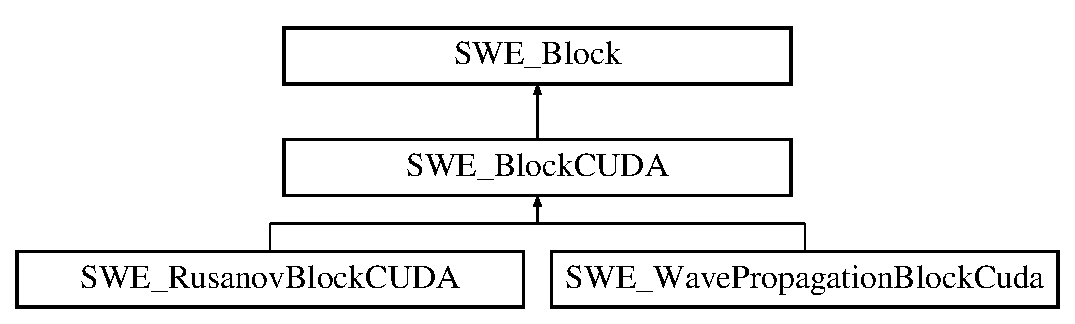
\includegraphics[height=3.000000cm]{classSWE__BlockCUDA}
\end{center}
\end{figure}
\subsection*{Public Member Functions}
\begin{DoxyCompactItemize}
\item 
\hyperlink{classSWE__BlockCUDA_a7e4f5f08cf6179d17e7ff64cb2f182d8}{S\-W\-E\-\_\-\-Block\-C\-U\-D\-A} (int l\-\_\-nx, int l\-\_\-ny, float l\-\_\-dx, float l\-\_\-dy)
\item 
virtual \hyperlink{classSWE__BlockCUDA_a37517831b7f36a9405eb566bc86e4243}{$\sim$\-S\-W\-E\-\_\-\-Block\-C\-U\-D\-A} ()
\item 
virtual \hyperlink{structSWE__Block1D}{S\-W\-E\-\_\-\-Block1\-D} $\ast$ \hyperlink{classSWE__BlockCUDA_a22782766fc679ac14e9ba30a4efc1688}{register\-Copy\-Layer} (\hyperlink{SWE__Scenario_8hh_aa5e01e3f7df312f7b9b0d02521141fcc}{Boundary\-Edge} edge)
\item 
virtual \hyperlink{structSWE__Block1D}{S\-W\-E\-\_\-\-Block1\-D} $\ast$ \hyperlink{classSWE__BlockCUDA_ab8671269d89d544a333a0b8c0fa72f37}{grab\-Ghost\-Layer} (\hyperlink{SWE__Scenario_8hh_aa5e01e3f7df312f7b9b0d02521141fcc}{Boundary\-Edge} edge)
\item 
const float $\ast$ \hyperlink{classSWE__BlockCUDA_a6d1b455840114ed08d785e17741e3015}{get\-C\-U\-D\-A\-\_\-water\-Height} ()
\item 
const float $\ast$ \hyperlink{classSWE__BlockCUDA_ad8bf853a1319ed215010dc05c78d33e6}{get\-C\-U\-D\-A\-\_\-bathymetry} ()
\end{DoxyCompactItemize}
\subsection*{Static Public Member Functions}
\begin{DoxyCompactItemize}
\item 
static void \hyperlink{classSWE__BlockCUDA_a73fceb94ac9c5ffc4164720967b06143}{print\-Device\-Information} ()
\item 
static void \hyperlink{classSWE__BlockCUDA_ad5143c0c87c6e28f84d446e3f93c0ec1}{init} (int i\-\_\-cuda\-Device=0)
\item 
static void \hyperlink{classSWE__BlockCUDA_a1d77f5dc1168bf11d1b10a92bcefa4ac}{finalize} ()
\end{DoxyCompactItemize}
\subsection*{Protected Member Functions}
\begin{DoxyCompactItemize}
\item 
virtual void \hyperlink{classSWE__BlockCUDA_a0876ef53f667c142d7d4dd9d01cfd2dc}{synch\-After\-Write} ()
\item 
virtual void \hyperlink{classSWE__BlockCUDA_ae54054af51e68415a68f3a1c7b25c139}{synch\-Water\-Height\-After\-Write} ()
\item 
virtual void \hyperlink{classSWE__BlockCUDA_a71b1d0b2e6959c298dfccf6a36264e13}{synch\-Discharge\-After\-Write} ()
\item 
virtual void \hyperlink{classSWE__BlockCUDA_aef79c805fec82b4d439642a758a8e95f}{synch\-Bathymetry\-After\-Write} ()
\item 
virtual void \hyperlink{classSWE__BlockCUDA_ab9cc911c9d67bcab9ecb2818a056930b}{synch\-Ghost\-Layer\-After\-Write} ()
\item 
virtual void \hyperlink{classSWE__BlockCUDA_a9ba846c6fa27734412d9fdfaa3823de2}{synch\-Before\-Read} ()
\item 
virtual void \hyperlink{classSWE__BlockCUDA_adfd3185b108632b2506558063714d7df}{synch\-Water\-Height\-Before\-Read} ()
\item 
virtual void \hyperlink{classSWE__BlockCUDA_adea7daf7794147d73d9465d37b37055e}{synch\-Discharge\-Before\-Read} ()
\item 
virtual void \hyperlink{classSWE__BlockCUDA_a3edd34c86eb0837d09f24cbf56a16e69}{synch\-Bathymetry\-Before\-Read} ()
\item 
virtual void \hyperlink{classSWE__BlockCUDA_a41d117ca8fe9a8c5509369edd026fd63}{synch\-Copy\-Layer\-Before\-Read} ()
\item 
virtual void \hyperlink{classSWE__BlockCUDA_a7cf66067cb7f023aadbd910051d389c8}{set\-Boundary\-Conditions} ()
\end{DoxyCompactItemize}
\subsection*{Protected Attributes}
\begin{DoxyCompactItemize}
\item 
\hypertarget{classSWE__BlockCUDA_a9c6a44214a75a9f5d4f8bb3806eaaf71}{float $\ast$ {\bfseries hd}}\label{classSWE__BlockCUDA_a9c6a44214a75a9f5d4f8bb3806eaaf71}

\item 
\hypertarget{classSWE__BlockCUDA_a2fb123601bbf091876dcccc351157c67}{float $\ast$ {\bfseries hud}}\label{classSWE__BlockCUDA_a2fb123601bbf091876dcccc351157c67}

\item 
\hypertarget{classSWE__BlockCUDA_a795fe87f7abfa7e6511232e03a808705}{float $\ast$ {\bfseries hvd}}\label{classSWE__BlockCUDA_a795fe87f7abfa7e6511232e03a808705}

\item 
\hypertarget{classSWE__BlockCUDA_ae08ee1752690e828a9e0470a3c55fb39}{float $\ast$ {\bfseries bd}}\label{classSWE__BlockCUDA_ae08ee1752690e828a9e0470a3c55fb39}

\end{DoxyCompactItemize}
\subsection*{Additional Inherited Members}


\subsection{Detailed Description}
\hyperlink{classSWE__BlockCUDA}{S\-W\-E\-\_\-\-Block\-C\-U\-D\-A} extends the base class \hyperlink{classSWE__Block}{S\-W\-E\-\_\-\-Block} towards a base class for a C\-U\-D\-A implementation of the shallow water equations. It adds the respective variables in G\-P\-U memory, and provides methods for data transfer between main and G\-P\-U memory. 

\subsection{Constructor \& Destructor Documentation}
\hypertarget{classSWE__BlockCUDA_a7e4f5f08cf6179d17e7ff64cb2f182d8}{\index{S\-W\-E\-\_\-\-Block\-C\-U\-D\-A@{S\-W\-E\-\_\-\-Block\-C\-U\-D\-A}!S\-W\-E\-\_\-\-Block\-C\-U\-D\-A@{S\-W\-E\-\_\-\-Block\-C\-U\-D\-A}}
\index{S\-W\-E\-\_\-\-Block\-C\-U\-D\-A@{S\-W\-E\-\_\-\-Block\-C\-U\-D\-A}!SWE_BlockCUDA@{S\-W\-E\-\_\-\-Block\-C\-U\-D\-A}}
\subsubsection[{S\-W\-E\-\_\-\-Block\-C\-U\-D\-A}]{\setlength{\rightskip}{0pt plus 5cm}S\-W\-E\-\_\-\-Block\-C\-U\-D\-A\-::\-S\-W\-E\-\_\-\-Block\-C\-U\-D\-A (
\begin{DoxyParamCaption}
\item[{int}]{l\-\_\-nx, }
\item[{int}]{l\-\_\-ny, }
\item[{float}]{l\-\_\-dx, }
\item[{float}]{l\-\_\-dy}
\end{DoxyParamCaption}
)}}\label{classSWE__BlockCUDA_a7e4f5f08cf6179d17e7ff64cb2f182d8}
Constructor\-: allocate variables for simulation

unknowns h,hu,hv,b are defined on grid indices \mbox{[}0,..,nx+1\mbox{]}$\ast$\mbox{[}0,..,ny+1\mbox{]} -\/$>$ computational domain is \mbox{[}1,..,nx\mbox{]}$\ast$\mbox{[}1,..,ny\mbox{]} -\/$>$ plus ghost cell layer

flux terms are defined for edges with indices \mbox{[}0,..,nx\mbox{]}$\ast$\mbox{[}1,..,ny\mbox{]} or \mbox{[}1,..,nx\mbox{]}$\ast$\href{for horizontal/vertical edges}{\tt 0,..,ny} Flux term with index (i,j) is located on the edge between cells with index (i,j) and (i+1,j) or (i,j+1)

bathymetry source terms are defined for cells with indices \mbox{[}1,..,nx\mbox{]}$\ast$\mbox{[}1,..,ny\mbox{]}


\begin{DoxyParams}{Parameters}
{\em i\-\_\-cuda\-Device} & I\-D of the C\-U\-D\-A-\/device, which should be used. \\
\hline
\end{DoxyParams}
\hypertarget{classSWE__BlockCUDA_a37517831b7f36a9405eb566bc86e4243}{\index{S\-W\-E\-\_\-\-Block\-C\-U\-D\-A@{S\-W\-E\-\_\-\-Block\-C\-U\-D\-A}!$\sim$\-S\-W\-E\-\_\-\-Block\-C\-U\-D\-A@{$\sim$\-S\-W\-E\-\_\-\-Block\-C\-U\-D\-A}}
\index{$\sim$\-S\-W\-E\-\_\-\-Block\-C\-U\-D\-A@{$\sim$\-S\-W\-E\-\_\-\-Block\-C\-U\-D\-A}!SWE_BlockCUDA@{S\-W\-E\-\_\-\-Block\-C\-U\-D\-A}}
\subsubsection[{$\sim$\-S\-W\-E\-\_\-\-Block\-C\-U\-D\-A}]{\setlength{\rightskip}{0pt plus 5cm}S\-W\-E\-\_\-\-Block\-C\-U\-D\-A\-::$\sim$\-S\-W\-E\-\_\-\-Block\-C\-U\-D\-A (
\begin{DoxyParamCaption}
{}
\end{DoxyParamCaption}
)\hspace{0.3cm}{\ttfamily [virtual]}}}\label{classSWE__BlockCUDA_a37517831b7f36a9405eb566bc86e4243}
Destructor\-: de-\/allocate all variables 

\subsection{Member Function Documentation}
\hypertarget{classSWE__BlockCUDA_a1d77f5dc1168bf11d1b10a92bcefa4ac}{\index{S\-W\-E\-\_\-\-Block\-C\-U\-D\-A@{S\-W\-E\-\_\-\-Block\-C\-U\-D\-A}!finalize@{finalize}}
\index{finalize@{finalize}!SWE_BlockCUDA@{S\-W\-E\-\_\-\-Block\-C\-U\-D\-A}}
\subsubsection[{finalize}]{\setlength{\rightskip}{0pt plus 5cm}void S\-W\-E\-\_\-\-Block\-C\-U\-D\-A\-::finalize (
\begin{DoxyParamCaption}
{}
\end{DoxyParamCaption}
)\hspace{0.3cm}{\ttfamily [static]}}}\label{classSWE__BlockCUDA_a1d77f5dc1168bf11d1b10a92bcefa4ac}
Cleans up the cuda device \hypertarget{classSWE__BlockCUDA_ad8bf853a1319ed215010dc05c78d33e6}{\index{S\-W\-E\-\_\-\-Block\-C\-U\-D\-A@{S\-W\-E\-\_\-\-Block\-C\-U\-D\-A}!get\-C\-U\-D\-A\-\_\-bathymetry@{get\-C\-U\-D\-A\-\_\-bathymetry}}
\index{get\-C\-U\-D\-A\-\_\-bathymetry@{get\-C\-U\-D\-A\-\_\-bathymetry}!SWE_BlockCUDA@{S\-W\-E\-\_\-\-Block\-C\-U\-D\-A}}
\subsubsection[{get\-C\-U\-D\-A\-\_\-bathymetry}]{\setlength{\rightskip}{0pt plus 5cm}const float$\ast$ S\-W\-E\-\_\-\-Block\-C\-U\-D\-A\-::get\-C\-U\-D\-A\-\_\-bathymetry (
\begin{DoxyParamCaption}
{}
\end{DoxyParamCaption}
)\hspace{0.3cm}{\ttfamily [inline]}}}\label{classSWE__BlockCUDA_ad8bf853a1319ed215010dc05c78d33e6}
\begin{DoxyReturn}{Returns}
pointer to the array \#hb (bathymetry) in device memory 
\end{DoxyReturn}
\hypertarget{classSWE__BlockCUDA_a6d1b455840114ed08d785e17741e3015}{\index{S\-W\-E\-\_\-\-Block\-C\-U\-D\-A@{S\-W\-E\-\_\-\-Block\-C\-U\-D\-A}!get\-C\-U\-D\-A\-\_\-water\-Height@{get\-C\-U\-D\-A\-\_\-water\-Height}}
\index{get\-C\-U\-D\-A\-\_\-water\-Height@{get\-C\-U\-D\-A\-\_\-water\-Height}!SWE_BlockCUDA@{S\-W\-E\-\_\-\-Block\-C\-U\-D\-A}}
\subsubsection[{get\-C\-U\-D\-A\-\_\-water\-Height}]{\setlength{\rightskip}{0pt plus 5cm}const float$\ast$ S\-W\-E\-\_\-\-Block\-C\-U\-D\-A\-::get\-C\-U\-D\-A\-\_\-water\-Height (
\begin{DoxyParamCaption}
{}
\end{DoxyParamCaption}
)\hspace{0.3cm}{\ttfamily [inline]}}}\label{classSWE__BlockCUDA_a6d1b455840114ed08d785e17741e3015}
\begin{DoxyReturn}{Returns}
pointer to the array \#hd (water height) in device memory 
\end{DoxyReturn}
\hypertarget{classSWE__BlockCUDA_ab8671269d89d544a333a0b8c0fa72f37}{\index{S\-W\-E\-\_\-\-Block\-C\-U\-D\-A@{S\-W\-E\-\_\-\-Block\-C\-U\-D\-A}!grab\-Ghost\-Layer@{grab\-Ghost\-Layer}}
\index{grab\-Ghost\-Layer@{grab\-Ghost\-Layer}!SWE_BlockCUDA@{S\-W\-E\-\_\-\-Block\-C\-U\-D\-A}}
\subsubsection[{grab\-Ghost\-Layer}]{\setlength{\rightskip}{0pt plus 5cm}{\bf S\-W\-E\-\_\-\-Block1\-D} $\ast$ S\-W\-E\-\_\-\-Block\-C\-U\-D\-A\-::grab\-Ghost\-Layer (
\begin{DoxyParamCaption}
\item[{{\bf Boundary\-Edge}}]{edge}
\end{DoxyParamCaption}
)\hspace{0.3cm}{\ttfamily [virtual]}}}\label{classSWE__BlockCUDA_ab8671269d89d544a333a0b8c0fa72f37}
\char`\"{}grab\char`\"{} the ghost layer at the specific boundary in order to set boundary values in this ghost layer externally. The boundary conditions at the respective ghost layer is set to P\-A\-S\-S\-I\-V\-E, such that the grabbing program component is responsible to provide correct values in the ghost layer, for example by receiving data from a remote copy layer via M\-P\-I communication. 
\begin{DoxyParams}{Parameters}
{\em specified} & edge \\
\hline
\end{DoxyParams}
\begin{DoxyReturn}{Returns}
a \hyperlink{structSWE__Block1D}{S\-W\-E\-\_\-\-Block1\-D} object that contains row variables h, hu, and hv 
\end{DoxyReturn}


Reimplemented from \hyperlink{classSWE__Block_a9a96c59444645e237d098803009158a3}{S\-W\-E\-\_\-\-Block}.

\hypertarget{classSWE__BlockCUDA_ad5143c0c87c6e28f84d446e3f93c0ec1}{\index{S\-W\-E\-\_\-\-Block\-C\-U\-D\-A@{S\-W\-E\-\_\-\-Block\-C\-U\-D\-A}!init@{init}}
\index{init@{init}!SWE_BlockCUDA@{S\-W\-E\-\_\-\-Block\-C\-U\-D\-A}}
\subsubsection[{init}]{\setlength{\rightskip}{0pt plus 5cm}void S\-W\-E\-\_\-\-Block\-C\-U\-D\-A\-::init (
\begin{DoxyParamCaption}
\item[{int}]{i\-\_\-cuda\-Device = {\ttfamily 0}}
\end{DoxyParamCaption}
)\hspace{0.3cm}{\ttfamily [static]}}}\label{classSWE__BlockCUDA_ad5143c0c87c6e28f84d446e3f93c0ec1}
Initializes the cuda device Has to be called once at the beginning. \hypertarget{classSWE__BlockCUDA_a73fceb94ac9c5ffc4164720967b06143}{\index{S\-W\-E\-\_\-\-Block\-C\-U\-D\-A@{S\-W\-E\-\_\-\-Block\-C\-U\-D\-A}!print\-Device\-Information@{print\-Device\-Information}}
\index{print\-Device\-Information@{print\-Device\-Information}!SWE_BlockCUDA@{S\-W\-E\-\_\-\-Block\-C\-U\-D\-A}}
\subsubsection[{print\-Device\-Information}]{\setlength{\rightskip}{0pt plus 5cm}void S\-W\-E\-\_\-\-Block\-C\-U\-D\-A\-::print\-Device\-Information (
\begin{DoxyParamCaption}
{}
\end{DoxyParamCaption}
)\hspace{0.3cm}{\ttfamily [static]}}}\label{classSWE__BlockCUDA_a73fceb94ac9c5ffc4164720967b06143}
Print some available information about the C\-U\-D\-A devices. id of the C\-U\-D\-A device.

total number of C\-U\-D\-A devices on this host.

drive and runtime version

device properties \hypertarget{classSWE__BlockCUDA_a22782766fc679ac14e9ba30a4efc1688}{\index{S\-W\-E\-\_\-\-Block\-C\-U\-D\-A@{S\-W\-E\-\_\-\-Block\-C\-U\-D\-A}!register\-Copy\-Layer@{register\-Copy\-Layer}}
\index{register\-Copy\-Layer@{register\-Copy\-Layer}!SWE_BlockCUDA@{S\-W\-E\-\_\-\-Block\-C\-U\-D\-A}}
\subsubsection[{register\-Copy\-Layer}]{\setlength{\rightskip}{0pt plus 5cm}{\bf S\-W\-E\-\_\-\-Block1\-D} $\ast$ S\-W\-E\-\_\-\-Block\-C\-U\-D\-A\-::register\-Copy\-Layer (
\begin{DoxyParamCaption}
\item[{{\bf Boundary\-Edge}}]{edge}
\end{DoxyParamCaption}
)\hspace{0.3cm}{\ttfamily [virtual]}}}\label{classSWE__BlockCUDA_a22782766fc679ac14e9ba30a4efc1688}
register the row or column layer next to a boundary as a \char`\"{}copy layer\char`\"{}, from which values will be copied into the ghost layer or a neighbour; \begin{DoxyReturn}{Returns}
a \hyperlink{structSWE__Block1D}{S\-W\-E\-\_\-\-Block1\-D} object that contains row variables h, hu, and hv 
\end{DoxyReturn}


Reimplemented from \hyperlink{classSWE__Block_a827ee5c61dc9c1b472ac8b4e1c19956a}{S\-W\-E\-\_\-\-Block}.

\hypertarget{classSWE__BlockCUDA_a7cf66067cb7f023aadbd910051d389c8}{\index{S\-W\-E\-\_\-\-Block\-C\-U\-D\-A@{S\-W\-E\-\_\-\-Block\-C\-U\-D\-A}!set\-Boundary\-Conditions@{set\-Boundary\-Conditions}}
\index{set\-Boundary\-Conditions@{set\-Boundary\-Conditions}!SWE_BlockCUDA@{S\-W\-E\-\_\-\-Block\-C\-U\-D\-A}}
\subsubsection[{set\-Boundary\-Conditions}]{\setlength{\rightskip}{0pt plus 5cm}void S\-W\-E\-\_\-\-Block\-C\-U\-D\-A\-::set\-Boundary\-Conditions (
\begin{DoxyParamCaption}
{}
\end{DoxyParamCaption}
)\hspace{0.3cm}{\ttfamily [protected]}, {\ttfamily [virtual]}}}\label{classSWE__BlockCUDA_a7cf66067cb7f023aadbd910051d389c8}
set the values of all ghost cells depending on the specifed boundary conditions 

Reimplemented from \hyperlink{classSWE__Block_a379807f0bf932b40aeb42065633fce60}{S\-W\-E\-\_\-\-Block}.

\hypertarget{classSWE__BlockCUDA_a0876ef53f667c142d7d4dd9d01cfd2dc}{\index{S\-W\-E\-\_\-\-Block\-C\-U\-D\-A@{S\-W\-E\-\_\-\-Block\-C\-U\-D\-A}!synch\-After\-Write@{synch\-After\-Write}}
\index{synch\-After\-Write@{synch\-After\-Write}!SWE_BlockCUDA@{S\-W\-E\-\_\-\-Block\-C\-U\-D\-A}}
\subsubsection[{synch\-After\-Write}]{\setlength{\rightskip}{0pt plus 5cm}void S\-W\-E\-\_\-\-Block\-C\-U\-D\-A\-::synch\-After\-Write (
\begin{DoxyParamCaption}
{}
\end{DoxyParamCaption}
)\hspace{0.3cm}{\ttfamily [protected]}, {\ttfamily [virtual]}}}\label{classSWE__BlockCUDA_a0876ef53f667c142d7d4dd9d01cfd2dc}
Update all temporary and non-\/local (for heterogeneous computing) variables after an external update of the main variables h, hu, hv, and b. 

Reimplemented from \hyperlink{classSWE__Block_ae914f9bf6d4ef8f974f9f005114985e7}{S\-W\-E\-\_\-\-Block}.

\hypertarget{classSWE__BlockCUDA_aef79c805fec82b4d439642a758a8e95f}{\index{S\-W\-E\-\_\-\-Block\-C\-U\-D\-A@{S\-W\-E\-\_\-\-Block\-C\-U\-D\-A}!synch\-Bathymetry\-After\-Write@{synch\-Bathymetry\-After\-Write}}
\index{synch\-Bathymetry\-After\-Write@{synch\-Bathymetry\-After\-Write}!SWE_BlockCUDA@{S\-W\-E\-\_\-\-Block\-C\-U\-D\-A}}
\subsubsection[{synch\-Bathymetry\-After\-Write}]{\setlength{\rightskip}{0pt plus 5cm}void S\-W\-E\-\_\-\-Block\-C\-U\-D\-A\-::synch\-Bathymetry\-After\-Write (
\begin{DoxyParamCaption}
{}
\end{DoxyParamCaption}
)\hspace{0.3cm}{\ttfamily [protected]}, {\ttfamily [virtual]}}}\label{classSWE__BlockCUDA_aef79c805fec82b4d439642a758a8e95f}
Update temporary and non-\/local (for heterogeneous computing) variables after an external update of the bathymetry b 

Reimplemented from \hyperlink{classSWE__Block_a4bece8aa90f67e55c40b91aab900febb}{S\-W\-E\-\_\-\-Block}.

\hypertarget{classSWE__BlockCUDA_a3edd34c86eb0837d09f24cbf56a16e69}{\index{S\-W\-E\-\_\-\-Block\-C\-U\-D\-A@{S\-W\-E\-\_\-\-Block\-C\-U\-D\-A}!synch\-Bathymetry\-Before\-Read@{synch\-Bathymetry\-Before\-Read}}
\index{synch\-Bathymetry\-Before\-Read@{synch\-Bathymetry\-Before\-Read}!SWE_BlockCUDA@{S\-W\-E\-\_\-\-Block\-C\-U\-D\-A}}
\subsubsection[{synch\-Bathymetry\-Before\-Read}]{\setlength{\rightskip}{0pt plus 5cm}void S\-W\-E\-\_\-\-Block\-C\-U\-D\-A\-::synch\-Bathymetry\-Before\-Read (
\begin{DoxyParamCaption}
{}
\end{DoxyParamCaption}
)\hspace{0.3cm}{\ttfamily [protected]}, {\ttfamily [virtual]}}}\label{classSWE__BlockCUDA_a3edd34c86eb0837d09f24cbf56a16e69}
Update temporary and non-\/local (for heterogeneous computing) variables before an external access to the bathymetry b 

Reimplemented from \hyperlink{classSWE__Block_a7c8258c6949518ca44f4e9ce89d33b09}{S\-W\-E\-\_\-\-Block}.

\hypertarget{classSWE__BlockCUDA_a9ba846c6fa27734412d9fdfaa3823de2}{\index{S\-W\-E\-\_\-\-Block\-C\-U\-D\-A@{S\-W\-E\-\_\-\-Block\-C\-U\-D\-A}!synch\-Before\-Read@{synch\-Before\-Read}}
\index{synch\-Before\-Read@{synch\-Before\-Read}!SWE_BlockCUDA@{S\-W\-E\-\_\-\-Block\-C\-U\-D\-A}}
\subsubsection[{synch\-Before\-Read}]{\setlength{\rightskip}{0pt plus 5cm}void S\-W\-E\-\_\-\-Block\-C\-U\-D\-A\-::synch\-Before\-Read (
\begin{DoxyParamCaption}
{}
\end{DoxyParamCaption}
)\hspace{0.3cm}{\ttfamily [protected]}, {\ttfamily [virtual]}}}\label{classSWE__BlockCUDA_a9ba846c6fa27734412d9fdfaa3823de2}
Update the main variables h, hu, hv, and b before an external read access\-: copies current content of the respective device variables hd, hud, hvd, bd 

Reimplemented from \hyperlink{classSWE__Block_a23d936cb9a4367092e5b2515f81fe819}{S\-W\-E\-\_\-\-Block}.

\hypertarget{classSWE__BlockCUDA_a41d117ca8fe9a8c5509369edd026fd63}{\index{S\-W\-E\-\_\-\-Block\-C\-U\-D\-A@{S\-W\-E\-\_\-\-Block\-C\-U\-D\-A}!synch\-Copy\-Layer\-Before\-Read@{synch\-Copy\-Layer\-Before\-Read}}
\index{synch\-Copy\-Layer\-Before\-Read@{synch\-Copy\-Layer\-Before\-Read}!SWE_BlockCUDA@{S\-W\-E\-\_\-\-Block\-C\-U\-D\-A}}
\subsubsection[{synch\-Copy\-Layer\-Before\-Read}]{\setlength{\rightskip}{0pt plus 5cm}void S\-W\-E\-\_\-\-Block\-C\-U\-D\-A\-::synch\-Copy\-Layer\-Before\-Read (
\begin{DoxyParamCaption}
{}
\end{DoxyParamCaption}
)\hspace{0.3cm}{\ttfamily [protected]}, {\ttfamily [virtual]}}}\label{classSWE__BlockCUDA_a41d117ca8fe9a8c5509369edd026fd63}
Update (for heterogeneous computing) variables h, hu, hv in copy layers before an external access to the unknowns (only required for P\-A\-S\-S\-I\-V\-E and C\-O\-N\-N\-E\-C\-T boundaries)
\begin{DoxyItemize}
\item copy (up-\/to-\/date) content from device memory into main memory 
\end{DoxyItemize}

Reimplemented from \hyperlink{classSWE__Block_a13c90d5a6596336013c41e73c8795f83}{S\-W\-E\-\_\-\-Block}.

\hypertarget{classSWE__BlockCUDA_a71b1d0b2e6959c298dfccf6a36264e13}{\index{S\-W\-E\-\_\-\-Block\-C\-U\-D\-A@{S\-W\-E\-\_\-\-Block\-C\-U\-D\-A}!synch\-Discharge\-After\-Write@{synch\-Discharge\-After\-Write}}
\index{synch\-Discharge\-After\-Write@{synch\-Discharge\-After\-Write}!SWE_BlockCUDA@{S\-W\-E\-\_\-\-Block\-C\-U\-D\-A}}
\subsubsection[{synch\-Discharge\-After\-Write}]{\setlength{\rightskip}{0pt plus 5cm}void S\-W\-E\-\_\-\-Block\-C\-U\-D\-A\-::synch\-Discharge\-After\-Write (
\begin{DoxyParamCaption}
{}
\end{DoxyParamCaption}
)\hspace{0.3cm}{\ttfamily [protected]}, {\ttfamily [virtual]}}}\label{classSWE__BlockCUDA_a71b1d0b2e6959c298dfccf6a36264e13}
Update temporary and non-\/local (for heterogeneous computing) variables after an external update of the discharge variables hu and hv 

Reimplemented from \hyperlink{classSWE__Block_a94c34030153178c9d94f3f14be174eaf}{S\-W\-E\-\_\-\-Block}.

\hypertarget{classSWE__BlockCUDA_adea7daf7794147d73d9465d37b37055e}{\index{S\-W\-E\-\_\-\-Block\-C\-U\-D\-A@{S\-W\-E\-\_\-\-Block\-C\-U\-D\-A}!synch\-Discharge\-Before\-Read@{synch\-Discharge\-Before\-Read}}
\index{synch\-Discharge\-Before\-Read@{synch\-Discharge\-Before\-Read}!SWE_BlockCUDA@{S\-W\-E\-\_\-\-Block\-C\-U\-D\-A}}
\subsubsection[{synch\-Discharge\-Before\-Read}]{\setlength{\rightskip}{0pt plus 5cm}void S\-W\-E\-\_\-\-Block\-C\-U\-D\-A\-::synch\-Discharge\-Before\-Read (
\begin{DoxyParamCaption}
{}
\end{DoxyParamCaption}
)\hspace{0.3cm}{\ttfamily [protected]}, {\ttfamily [virtual]}}}\label{classSWE__BlockCUDA_adea7daf7794147d73d9465d37b37055e}
Update temporary and non-\/local (for heterogeneous computing) variables before an external access to the discharge variables hu and hv 

Reimplemented from \hyperlink{classSWE__Block_a3773dcb194212fb8cb40ab8465575aa1}{S\-W\-E\-\_\-\-Block}.

\hypertarget{classSWE__BlockCUDA_ab9cc911c9d67bcab9ecb2818a056930b}{\index{S\-W\-E\-\_\-\-Block\-C\-U\-D\-A@{S\-W\-E\-\_\-\-Block\-C\-U\-D\-A}!synch\-Ghost\-Layer\-After\-Write@{synch\-Ghost\-Layer\-After\-Write}}
\index{synch\-Ghost\-Layer\-After\-Write@{synch\-Ghost\-Layer\-After\-Write}!SWE_BlockCUDA@{S\-W\-E\-\_\-\-Block\-C\-U\-D\-A}}
\subsubsection[{synch\-Ghost\-Layer\-After\-Write}]{\setlength{\rightskip}{0pt plus 5cm}void S\-W\-E\-\_\-\-Block\-C\-U\-D\-A\-::synch\-Ghost\-Layer\-After\-Write (
\begin{DoxyParamCaption}
{}
\end{DoxyParamCaption}
)\hspace{0.3cm}{\ttfamily [protected]}, {\ttfamily [virtual]}}}\label{classSWE__BlockCUDA_ab9cc911c9d67bcab9ecb2818a056930b}
synchronise the ghost layer content of h, hu, and hv in main memory with device memory and auxiliary data structures, i.\-e. transfer memory from main/auxiliary memory into device memory 

Reimplemented from \hyperlink{classSWE__Block_a4657993ebdb5f0132b077e63790d0b2b}{S\-W\-E\-\_\-\-Block}.

\hypertarget{classSWE__BlockCUDA_ae54054af51e68415a68f3a1c7b25c139}{\index{S\-W\-E\-\_\-\-Block\-C\-U\-D\-A@{S\-W\-E\-\_\-\-Block\-C\-U\-D\-A}!synch\-Water\-Height\-After\-Write@{synch\-Water\-Height\-After\-Write}}
\index{synch\-Water\-Height\-After\-Write@{synch\-Water\-Height\-After\-Write}!SWE_BlockCUDA@{S\-W\-E\-\_\-\-Block\-C\-U\-D\-A}}
\subsubsection[{synch\-Water\-Height\-After\-Write}]{\setlength{\rightskip}{0pt plus 5cm}void S\-W\-E\-\_\-\-Block\-C\-U\-D\-A\-::synch\-Water\-Height\-After\-Write (
\begin{DoxyParamCaption}
{}
\end{DoxyParamCaption}
)\hspace{0.3cm}{\ttfamily [protected]}, {\ttfamily [virtual]}}}\label{classSWE__BlockCUDA_ae54054af51e68415a68f3a1c7b25c139}
Update temporary and non-\/local (for heterogeneous computing) variables after an external update of the water height h 

Reimplemented from \hyperlink{classSWE__Block_aa2924833e29a795d8c04fb79bfe794de}{S\-W\-E\-\_\-\-Block}.

\hypertarget{classSWE__BlockCUDA_adfd3185b108632b2506558063714d7df}{\index{S\-W\-E\-\_\-\-Block\-C\-U\-D\-A@{S\-W\-E\-\_\-\-Block\-C\-U\-D\-A}!synch\-Water\-Height\-Before\-Read@{synch\-Water\-Height\-Before\-Read}}
\index{synch\-Water\-Height\-Before\-Read@{synch\-Water\-Height\-Before\-Read}!SWE_BlockCUDA@{S\-W\-E\-\_\-\-Block\-C\-U\-D\-A}}
\subsubsection[{synch\-Water\-Height\-Before\-Read}]{\setlength{\rightskip}{0pt plus 5cm}void S\-W\-E\-\_\-\-Block\-C\-U\-D\-A\-::synch\-Water\-Height\-Before\-Read (
\begin{DoxyParamCaption}
{}
\end{DoxyParamCaption}
)\hspace{0.3cm}{\ttfamily [protected]}, {\ttfamily [virtual]}}}\label{classSWE__BlockCUDA_adfd3185b108632b2506558063714d7df}
Update temporary and non-\/local (for heterogeneous computing) variables before an external access to the water height h 

Reimplemented from \hyperlink{classSWE__Block_a07c85681ab29106c3b164db969899ace}{S\-W\-E\-\_\-\-Block}.



The documentation for this class was generated from the following files\-:\begin{DoxyCompactItemize}
\item 
/home/sascha/\-Dokumente/\-Projects/\-Tsun\-Sim/\-S\-W\-E/src/blocks/cuda/\hyperlink{SWE__BlockCUDA_8hh}{S\-W\-E\-\_\-\-Block\-C\-U\-D\-A.\-hh}\item 
/home/sascha/\-Dokumente/\-Projects/\-Tsun\-Sim/\-S\-W\-E/src/blocks/cuda/\hyperlink{SWE__BlockCUDA_8cu}{S\-W\-E\-\_\-\-Block\-C\-U\-D\-A.\-cu}\end{DoxyCompactItemize}

\hypertarget{classSWE__DimensionalSplitting}{\section{S\-W\-E\-\_\-\-Dimensional\-Splitting Class Reference}
\label{classSWE__DimensionalSplitting}\index{S\-W\-E\-\_\-\-Dimensional\-Splitting@{S\-W\-E\-\_\-\-Dimensional\-Splitting}}
}


{\ttfamily \#include $<$S\-W\-E\-\_\-\-Dimensional\-Splitting.\-hpp$>$}

Inheritance diagram for S\-W\-E\-\_\-\-Dimensional\-Splitting\-:\begin{figure}[H]
\begin{center}
\leavevmode
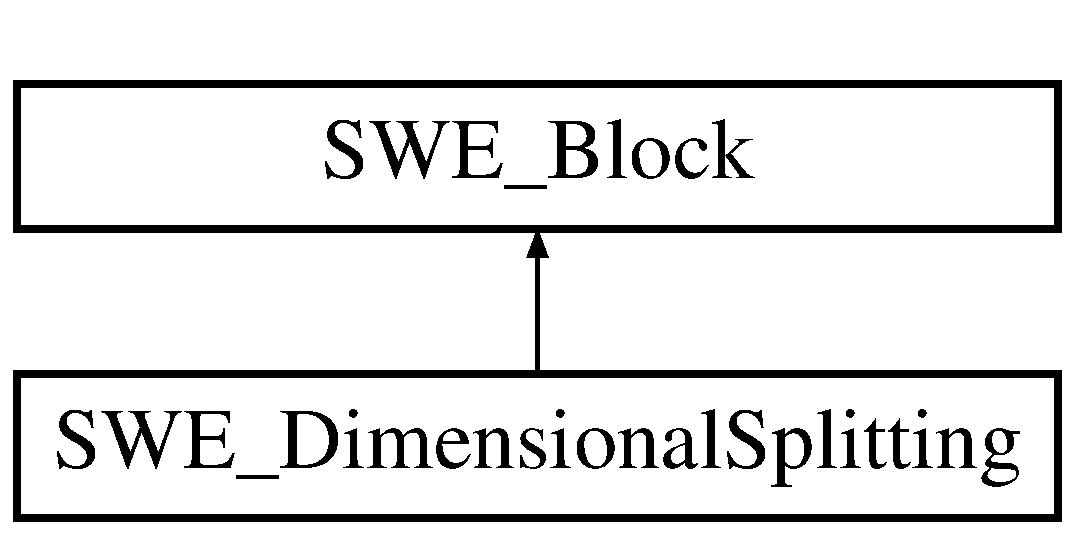
\includegraphics[height=2.000000cm]{classSWE__DimensionalSplitting}
\end{center}
\end{figure}
\subsection*{Public Member Functions}
\begin{DoxyCompactItemize}
\item 
\hyperlink{classSWE__DimensionalSplitting_a3ab0c9de647ca241dbab1aa02cc42a04}{S\-W\-E\-\_\-\-Dimensional\-Splitting} (int l\-\_\-nx, int l\-\_\-ny, float l\-\_\-dx, float l\-\_\-dy)
\item 
void \hyperlink{classSWE__DimensionalSplitting_a84759f8fbbbfe1e46613375515826f0f}{compute\-Numerical\-Fluxes} ()
\item 
void \hyperlink{classSWE__DimensionalSplitting_af74b527ff9ca7727442db92d2e438531}{update\-Unknowns} (float dt)
\end{DoxyCompactItemize}
\subsection*{Additional Inherited Members}


\subsection{Detailed Description}
This class implements \hyperlink{classSWE__Block}{S\-W\-E\-\_\-\-Block} using the dimensional splitting approach and the F-\/\-Wave solver 

\subsection{Constructor \& Destructor Documentation}
\hypertarget{classSWE__DimensionalSplitting_a3ab0c9de647ca241dbab1aa02cc42a04}{\index{S\-W\-E\-\_\-\-Dimensional\-Splitting@{S\-W\-E\-\_\-\-Dimensional\-Splitting}!S\-W\-E\-\_\-\-Dimensional\-Splitting@{S\-W\-E\-\_\-\-Dimensional\-Splitting}}
\index{S\-W\-E\-\_\-\-Dimensional\-Splitting@{S\-W\-E\-\_\-\-Dimensional\-Splitting}!SWE_DimensionalSplitting@{S\-W\-E\-\_\-\-Dimensional\-Splitting}}
\subsubsection[{S\-W\-E\-\_\-\-Dimensional\-Splitting}]{\setlength{\rightskip}{0pt plus 5cm}S\-W\-E\-\_\-\-Dimensional\-Splitting\-::\-S\-W\-E\-\_\-\-Dimensional\-Splitting (
\begin{DoxyParamCaption}
\item[{int}]{l\-\_\-nx, }
\item[{int}]{l\-\_\-ny, }
\item[{float}]{l\-\_\-dx, }
\item[{float}]{l\-\_\-dy}
\end{DoxyParamCaption}
)\hspace{0.3cm}{\ttfamily [inline]}}}\label{classSWE__DimensionalSplitting_a3ab0c9de647ca241dbab1aa02cc42a04}
Constructor


\begin{DoxyParams}{Parameters}
{\em l\-\_\-nx} & x dimension of the domain \\
\hline
{\em l\-\_\-ny} & y dimension of the domain \\
\hline
{\em l\-\_\-dx} & cell size in x dimension \\
\hline
{\em l\-\_\-dy} & cell size in y dimension \\
\hline
\end{DoxyParams}


\subsection{Member Function Documentation}
\hypertarget{classSWE__DimensionalSplitting_a84759f8fbbbfe1e46613375515826f0f}{\index{S\-W\-E\-\_\-\-Dimensional\-Splitting@{S\-W\-E\-\_\-\-Dimensional\-Splitting}!compute\-Numerical\-Fluxes@{compute\-Numerical\-Fluxes}}
\index{compute\-Numerical\-Fluxes@{compute\-Numerical\-Fluxes}!SWE_DimensionalSplitting@{S\-W\-E\-\_\-\-Dimensional\-Splitting}}
\subsubsection[{compute\-Numerical\-Fluxes}]{\setlength{\rightskip}{0pt plus 5cm}void S\-W\-E\-\_\-\-Dimensional\-Splitting\-::compute\-Numerical\-Fluxes (
\begin{DoxyParamCaption}
{}
\end{DoxyParamCaption}
)\hspace{0.3cm}{\ttfamily [inline]}, {\ttfamily [virtual]}}}\label{classSWE__DimensionalSplitting_a84759f8fbbbfe1e46613375515826f0f}
computing the net updates A\-N\-D applying them already 

Implements \hyperlink{classSWE__Block_a94dcf2c6ae31731e4586e45628b0c00e}{S\-W\-E\-\_\-\-Block}.

\hypertarget{classSWE__DimensionalSplitting_af74b527ff9ca7727442db92d2e438531}{\index{S\-W\-E\-\_\-\-Dimensional\-Splitting@{S\-W\-E\-\_\-\-Dimensional\-Splitting}!update\-Unknowns@{update\-Unknowns}}
\index{update\-Unknowns@{update\-Unknowns}!SWE_DimensionalSplitting@{S\-W\-E\-\_\-\-Dimensional\-Splitting}}
\subsubsection[{update\-Unknowns}]{\setlength{\rightskip}{0pt plus 5cm}void S\-W\-E\-\_\-\-Dimensional\-Splitting\-::update\-Unknowns (
\begin{DoxyParamCaption}
\item[{float}]{dt}
\end{DoxyParamCaption}
)\hspace{0.3cm}{\ttfamily [inline]}, {\ttfamily [virtual]}}}\label{classSWE__DimensionalSplitting_af74b527ff9ca7727442db92d2e438531}
Applying the net updates (C\-A\-R\-E\-: Compute\-Numerical\-Fluxes already calls this, don't use it again) 

Implements \hyperlink{classSWE__Block_ab2b4b659f23d5d45413dece8d2da3298}{S\-W\-E\-\_\-\-Block}.



The documentation for this class was generated from the following file\-:\begin{DoxyCompactItemize}
\item 
/home/sascha/\-Dokumente/\-Projects/\-Tsun\-Sim/\-S\-W\-E/src/blocks/\hyperlink{SWE__DimensionalSplitting_8hpp}{S\-W\-E\-\_\-\-Dimensional\-Splitting.\-hpp}\end{DoxyCompactItemize}

\hypertarget{classSWE__RadialDamBreakScenario}{\section{S\-W\-E\-\_\-\-Radial\-Dam\-Break\-Scenario Class Reference}
\label{classSWE__RadialDamBreakScenario}\index{S\-W\-E\-\_\-\-Radial\-Dam\-Break\-Scenario@{S\-W\-E\-\_\-\-Radial\-Dam\-Break\-Scenario}}
}


{\ttfamily \#include $<$S\-W\-E\-\_\-simple\-\_\-scenarios.\-hh$>$}

Inheritance diagram for S\-W\-E\-\_\-\-Radial\-Dam\-Break\-Scenario\-:\begin{figure}[H]
\begin{center}
\leavevmode
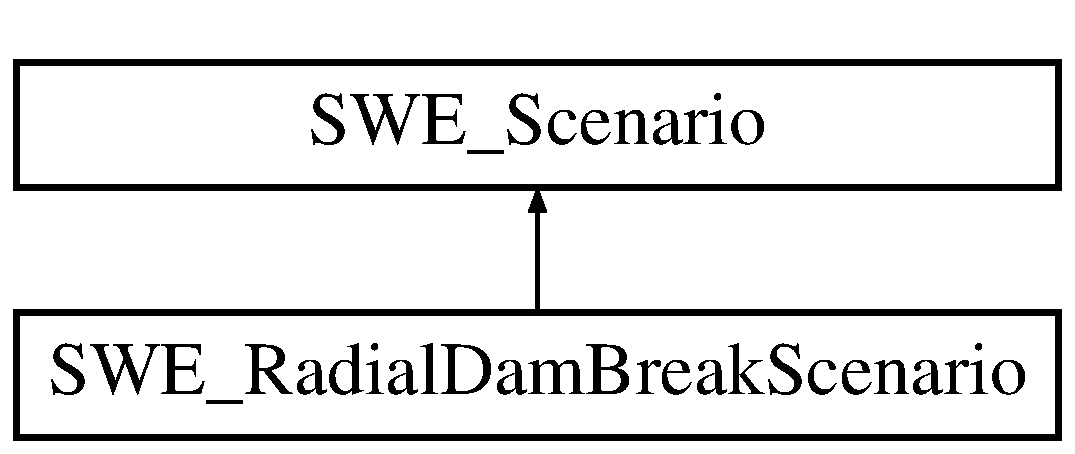
\includegraphics[height=2.000000cm]{classSWE__RadialDamBreakScenario}
\end{center}
\end{figure}
\subsection*{Public Member Functions}
\begin{DoxyCompactItemize}
\item 
\hypertarget{classSWE__RadialDamBreakScenario_ab54c88d18ff3a577a3e33f1659d97b50}{float {\bfseries get\-Bathymetry} (float x, float y)}\label{classSWE__RadialDamBreakScenario_ab54c88d18ff3a577a3e33f1659d97b50}

\item 
\hypertarget{classSWE__RadialDamBreakScenario_a0fb0917dd1e47f9580bd94ba5816795c}{float {\bfseries get\-Water\-Height} (float x, float y)}\label{classSWE__RadialDamBreakScenario_a0fb0917dd1e47f9580bd94ba5816795c}

\item 
\hypertarget{classSWE__RadialDamBreakScenario_a5e118a3d34aace3175745965d5d9c567}{virtual float {\bfseries end\-Simulation} ()}\label{classSWE__RadialDamBreakScenario_a5e118a3d34aace3175745965d5d9c567}

\item 
\hypertarget{classSWE__RadialDamBreakScenario_a40a7ddfd7d85631eeb708232c9f7f20d}{virtual \hyperlink{SWE__Scenario_8hh_af75d5dd7322fa39ed0af4e7839e600f8}{Boundary\-Type} {\bfseries get\-Boundary\-Type} (\hyperlink{SWE__Scenario_8hh_aa5e01e3f7df312f7b9b0d02521141fcc}{Boundary\-Edge} edge)}\label{classSWE__RadialDamBreakScenario_a40a7ddfd7d85631eeb708232c9f7f20d}

\item 
float \hyperlink{classSWE__RadialDamBreakScenario_ac5392df630c8164560df5cb902df385a}{get\-Boundary\-Pos} (\hyperlink{SWE__Scenario_8hh_aa5e01e3f7df312f7b9b0d02521141fcc}{Boundary\-Edge} i\-\_\-edge)
\end{DoxyCompactItemize}
\subsection*{Additional Inherited Members}


\subsection{Detailed Description}
Scenario \char`\"{}\-Radial Dam Break\char`\"{}\-: elevated water in the center of the domain 

\subsection{Member Function Documentation}
\hypertarget{classSWE__RadialDamBreakScenario_ac5392df630c8164560df5cb902df385a}{\index{S\-W\-E\-\_\-\-Radial\-Dam\-Break\-Scenario@{S\-W\-E\-\_\-\-Radial\-Dam\-Break\-Scenario}!get\-Boundary\-Pos@{get\-Boundary\-Pos}}
\index{get\-Boundary\-Pos@{get\-Boundary\-Pos}!SWE_RadialDamBreakScenario@{S\-W\-E\-\_\-\-Radial\-Dam\-Break\-Scenario}}
\subsubsection[{get\-Boundary\-Pos}]{\setlength{\rightskip}{0pt plus 5cm}float S\-W\-E\-\_\-\-Radial\-Dam\-Break\-Scenario\-::get\-Boundary\-Pos (
\begin{DoxyParamCaption}
\item[{{\bf Boundary\-Edge}}]{i\-\_\-edge}
\end{DoxyParamCaption}
)\hspace{0.3cm}{\ttfamily [inline]}, {\ttfamily [virtual]}}}\label{classSWE__RadialDamBreakScenario_ac5392df630c8164560df5cb902df385a}
Get the boundary positions


\begin{DoxyParams}{Parameters}
{\em i\-\_\-edge} & which edge \\
\hline
\end{DoxyParams}
\begin{DoxyReturn}{Returns}
value in the corresponding dimension 
\end{DoxyReturn}


Reimplemented from \hyperlink{classSWE__Scenario}{S\-W\-E\-\_\-\-Scenario}.



The documentation for this class was generated from the following file\-:\begin{DoxyCompactItemize}
\item 
/home/sascha/\-Dokumente/\-Projects/\-Tsun\-Sim/\-S\-W\-E/src/scenarios/\hyperlink{SWE__simple__scenarios_8hh}{S\-W\-E\-\_\-simple\-\_\-scenarios.\-hh}\end{DoxyCompactItemize}

\hypertarget{classSWE__RusanovBlock}{\section{S\-W\-E\-\_\-\-Rusanov\-Block Class Reference}
\label{classSWE__RusanovBlock}\index{S\-W\-E\-\_\-\-Rusanov\-Block@{S\-W\-E\-\_\-\-Rusanov\-Block}}
}


{\ttfamily \#include $<$S\-W\-E\-\_\-\-Rusanov\-Block.\-hh$>$}

Inheritance diagram for S\-W\-E\-\_\-\-Rusanov\-Block\-:\begin{figure}[H]
\begin{center}
\leavevmode
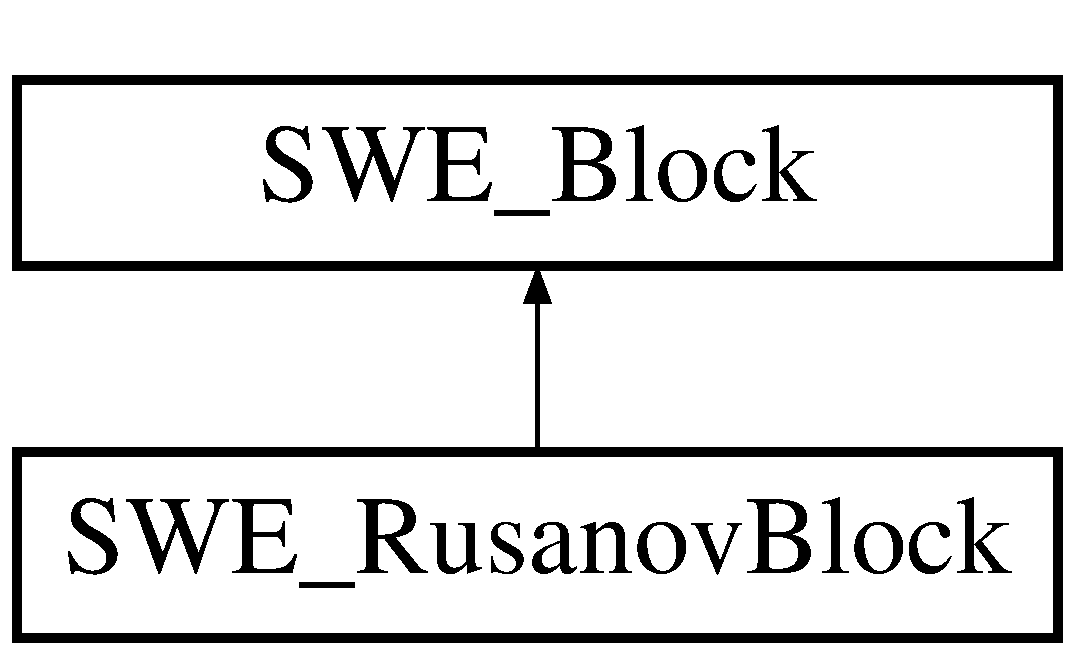
\includegraphics[height=2.000000cm]{classSWE__RusanovBlock}
\end{center}
\end{figure}
\subsection*{Public Member Functions}
\begin{DoxyCompactItemize}
\item 
\hyperlink{classSWE__RusanovBlock_a479a282899300076c44ccabcb42b5b5c}{S\-W\-E\-\_\-\-Rusanov\-Block} (float \-\_\-offset\-X=0, float \-\_\-offset\-Y=0)
\item 
virtual \hyperlink{classSWE__RusanovBlock_aab12f79b94c8ac3cc541ceb2814f72d4}{$\sim$\-S\-W\-E\-\_\-\-Rusanov\-Block} ()
\item 
virtual void \hyperlink{classSWE__RusanovBlock_ada062db4f54700011d50378b0045830a}{simulate\-Timestep} (float dt)
\begin{DoxyCompactList}\small\item\em execute a single time step of the simulation \end{DoxyCompactList}\item 
virtual float \hyperlink{classSWE__RusanovBlock_a645322106b3e5b6f0cca077611ad2159}{simulate} (float t\-Start, float t\-End)
\begin{DoxyCompactList}\small\item\em compute simulate from specified start to end time \end{DoxyCompactList}\item 
virtual void \hyperlink{classSWE__RusanovBlock_a78cdefa510cd2d88ca4e213f75b9b10b}{compute\-Numerical\-Fluxes} ()
\begin{DoxyCompactList}\small\item\em compute flux terms on edges \end{DoxyCompactList}\item 
virtual void \hyperlink{classSWE__RusanovBlock_a2980aa21030ba8fc607001ad817d7454}{update\-Unknowns} (float dt)
\begin{DoxyCompactList}\small\item\em update unknowns according to fluxes (Euler time step) \end{DoxyCompactList}\end{DoxyCompactItemize}
\subsection*{Protected Member Functions}
\begin{DoxyCompactItemize}
\item 
virtual void \hyperlink{classSWE__RusanovBlock_ac7306305d9c39e418301fc588693c88b}{compute\-Bathymetry\-Sources} ()
\begin{DoxyCompactList}\small\item\em compute source terms \end{DoxyCompactList}\item 
float \hyperlink{classSWE__RusanovBlock_a5a2f154dd2110e8515829564dd806530}{compute\-Local\-S\-V} (int i, int j, char dir)
\item 
\hypertarget{classSWE__RusanovBlock_a88b3537e5dbe509b0b7495b8e28275bf}{virtual void {\bfseries compute\-Max\-Timestep} ()}\label{classSWE__RusanovBlock_a88b3537e5dbe509b0b7495b8e28275bf}

\end{DoxyCompactItemize}
\subsection*{Static Protected Member Functions}
\begin{DoxyCompactItemize}
\item 
static float \hyperlink{classSWE__RusanovBlock_a37c4e0d841054a32adaa8ab26fb7c208}{compute\-Flux} (float f\-Loc, float f\-Neigh, float xi\-Loc, float xi\-Neigh, float llf)
\end{DoxyCompactItemize}
\subsection*{Protected Attributes}
\begin{DoxyCompactItemize}
\item 
\hypertarget{classSWE__RusanovBlock_a13e147a6a4f8b39e1a95f37372a04d5b}{\hyperlink{classFloat2D}{Float2\-D} {\bfseries Fh}}\label{classSWE__RusanovBlock_a13e147a6a4f8b39e1a95f37372a04d5b}

\item 
\hypertarget{classSWE__RusanovBlock_a945f257acfa7b05dd0989c9525160b0b}{\hyperlink{classFloat2D}{Float2\-D} {\bfseries Fhu}}\label{classSWE__RusanovBlock_a945f257acfa7b05dd0989c9525160b0b}

\item 
\hypertarget{classSWE__RusanovBlock_a788982f2b64f97d271291ef7df669c57}{\hyperlink{classFloat2D}{Float2\-D} {\bfseries Fhv}}\label{classSWE__RusanovBlock_a788982f2b64f97d271291ef7df669c57}

\item 
\hypertarget{classSWE__RusanovBlock_aaa1d9c2b8f3dc1afe0f818bade7c3940}{\hyperlink{classFloat2D}{Float2\-D} {\bfseries Gh}}\label{classSWE__RusanovBlock_aaa1d9c2b8f3dc1afe0f818bade7c3940}

\item 
\hypertarget{classSWE__RusanovBlock_af479e7882925550951da40ce85736f83}{\hyperlink{classFloat2D}{Float2\-D} {\bfseries Ghu}}\label{classSWE__RusanovBlock_af479e7882925550951da40ce85736f83}

\item 
\hypertarget{classSWE__RusanovBlock_a2f856e0d68708748451c9ca1f166aa79}{\hyperlink{classFloat2D}{Float2\-D} {\bfseries Ghv}}\label{classSWE__RusanovBlock_a2f856e0d68708748451c9ca1f166aa79}

\item 
\hypertarget{classSWE__RusanovBlock_af6f73bf8459849ad75c1d7e70b279710}{\hyperlink{classFloat2D}{Float2\-D} {\bfseries Bx}}\label{classSWE__RusanovBlock_af6f73bf8459849ad75c1d7e70b279710}

\item 
\hypertarget{classSWE__RusanovBlock_a0c044eadcc80059b8708cf8f8c77add1}{\hyperlink{classFloat2D}{Float2\-D} {\bfseries By}}\label{classSWE__RusanovBlock_a0c044eadcc80059b8708cf8f8c77add1}

\end{DoxyCompactItemize}
\subsection*{Friends}
\begin{DoxyCompactItemize}
\item 
ostream \& \hyperlink{classSWE__RusanovBlock_a11f96afabd5e590e50d491568b96503a}{operator$<$$<$} (ostream \&os, const \hyperlink{classSWE__RusanovBlock}{S\-W\-E\-\_\-\-Rusanov\-Block} \&swe)
\end{DoxyCompactItemize}
\subsection*{Additional Inherited Members}


\subsection{Detailed Description}
\hyperlink{classSWE__RusanovBlock}{S\-W\-E\-\_\-\-Rusanov\-Block} is an implementation of the \hyperlink{classSWE__Block}{S\-W\-E\-\_\-\-Block} abstract class. It uses a simple Rusanov flux (aka local Lax-\/\-Friedrich) in the model, with some simple modifications to obtain a well-\/balanced scheme. 

\subsection{Constructor \& Destructor Documentation}
\hypertarget{classSWE__RusanovBlock_a479a282899300076c44ccabcb42b5b5c}{\index{S\-W\-E\-\_\-\-Rusanov\-Block@{S\-W\-E\-\_\-\-Rusanov\-Block}!S\-W\-E\-\_\-\-Rusanov\-Block@{S\-W\-E\-\_\-\-Rusanov\-Block}}
\index{S\-W\-E\-\_\-\-Rusanov\-Block@{S\-W\-E\-\_\-\-Rusanov\-Block}!SWE_RusanovBlock@{S\-W\-E\-\_\-\-Rusanov\-Block}}
\subsubsection[{S\-W\-E\-\_\-\-Rusanov\-Block}]{\setlength{\rightskip}{0pt plus 5cm}S\-W\-E\-\_\-\-Rusanov\-Block\-::\-S\-W\-E\-\_\-\-Rusanov\-Block (
\begin{DoxyParamCaption}
\item[{float}]{\-\_\-offset\-X = {\ttfamily 0}, }
\item[{float}]{\-\_\-offset\-Y = {\ttfamily 0}}
\end{DoxyParamCaption}
)}}\label{classSWE__RusanovBlock_a479a282899300076c44ccabcb42b5b5c}
Constructor\-: allocate variables for simulation

unknowns h,hu,hv,b are defined on grid indices \mbox{[}0,..,nx+1\mbox{]}$\ast$\mbox{[}0,..,ny+1\mbox{]} -\/$>$ computational domain is \mbox{[}1,..,nx\mbox{]}$\ast$\mbox{[}1,..,ny\mbox{]} -\/$>$ plus ghost cell layer

flux terms are defined for edges with indices \mbox{[}0,..,nx\mbox{]}$\ast$\mbox{[}1,..,ny\mbox{]} or \mbox{[}1,..,nx\mbox{]}$\ast$\href{for horizontal/vertical edges}{\tt 0,..,ny} Flux term with index (i,j) is located on the edge between cells with index (i,j) and (i+1,j) or (i,j+1)

bathymetry source terms are defined for cells with indices \mbox{[}1,..,nx\mbox{]}$\ast$\mbox{[}1,..,ny\mbox{]}

@ param \-\_\-offset\-X x coordinate of block origin @ param \-\_\-offset\-Y y coordinate of block origin \hypertarget{classSWE__RusanovBlock_aab12f79b94c8ac3cc541ceb2814f72d4}{\index{S\-W\-E\-\_\-\-Rusanov\-Block@{S\-W\-E\-\_\-\-Rusanov\-Block}!$\sim$\-S\-W\-E\-\_\-\-Rusanov\-Block@{$\sim$\-S\-W\-E\-\_\-\-Rusanov\-Block}}
\index{$\sim$\-S\-W\-E\-\_\-\-Rusanov\-Block@{$\sim$\-S\-W\-E\-\_\-\-Rusanov\-Block}!SWE_RusanovBlock@{S\-W\-E\-\_\-\-Rusanov\-Block}}
\subsubsection[{$\sim$\-S\-W\-E\-\_\-\-Rusanov\-Block}]{\setlength{\rightskip}{0pt plus 5cm}S\-W\-E\-\_\-\-Rusanov\-Block\-::$\sim$\-S\-W\-E\-\_\-\-Rusanov\-Block (
\begin{DoxyParamCaption}
{}
\end{DoxyParamCaption}
)\hspace{0.3cm}{\ttfamily [virtual]}}}\label{classSWE__RusanovBlock_aab12f79b94c8ac3cc541ceb2814f72d4}
Destructor\-: de-\/allocate all variables 

\subsection{Member Function Documentation}
\hypertarget{classSWE__RusanovBlock_ac7306305d9c39e418301fc588693c88b}{\index{S\-W\-E\-\_\-\-Rusanov\-Block@{S\-W\-E\-\_\-\-Rusanov\-Block}!compute\-Bathymetry\-Sources@{compute\-Bathymetry\-Sources}}
\index{compute\-Bathymetry\-Sources@{compute\-Bathymetry\-Sources}!SWE_RusanovBlock@{S\-W\-E\-\_\-\-Rusanov\-Block}}
\subsubsection[{compute\-Bathymetry\-Sources}]{\setlength{\rightskip}{0pt plus 5cm}void S\-W\-E\-\_\-\-Rusanov\-Block\-::compute\-Bathymetry\-Sources (
\begin{DoxyParamCaption}
{}
\end{DoxyParamCaption}
)\hspace{0.3cm}{\ttfamily [protected]}, {\ttfamily [virtual]}}}\label{classSWE__RusanovBlock_ac7306305d9c39e418301fc588693c88b}


compute source terms 

compute the bathymetry source terms in all cells \hypertarget{classSWE__RusanovBlock_a37c4e0d841054a32adaa8ab26fb7c208}{\index{S\-W\-E\-\_\-\-Rusanov\-Block@{S\-W\-E\-\_\-\-Rusanov\-Block}!compute\-Flux@{compute\-Flux}}
\index{compute\-Flux@{compute\-Flux}!SWE_RusanovBlock@{S\-W\-E\-\_\-\-Rusanov\-Block}}
\subsubsection[{compute\-Flux}]{\setlength{\rightskip}{0pt plus 5cm}float S\-W\-E\-\_\-\-Rusanov\-Block\-::compute\-Flux (
\begin{DoxyParamCaption}
\item[{float}]{f\-Low, }
\item[{float}]{f\-High, }
\item[{float}]{xi\-Low, }
\item[{float}]{xi\-High, }
\item[{float}]{llf}
\end{DoxyParamCaption}
)\hspace{0.3cm}{\ttfamily [static]}, {\ttfamily [protected]}}}\label{classSWE__RusanovBlock_a37c4e0d841054a32adaa8ab26fb7c208}
compute the flux term on a given edge (acc. to local Lax-\/\-Friedrich method aka Rusanov flux)\-: f\-Low and f\-High contain the values of the flux function in the two adjacent grid cells xi\-Low and xi\-High are the values of the unknowns in the two adjacent grid cells \char`\"{}\-Low\char`\"{} represents the cell with lower i/j index (\char`\"{}\-High\char`\"{} for larger index). llf should contain the local signal velocity (as compute by compute\-Local\-S\-V) for llf=dx/dt (or dy/dt), we obtain the standard Lax Friedrich method \hypertarget{classSWE__RusanovBlock_a5a2f154dd2110e8515829564dd806530}{\index{S\-W\-E\-\_\-\-Rusanov\-Block@{S\-W\-E\-\_\-\-Rusanov\-Block}!compute\-Local\-S\-V@{compute\-Local\-S\-V}}
\index{compute\-Local\-S\-V@{compute\-Local\-S\-V}!SWE_RusanovBlock@{S\-W\-E\-\_\-\-Rusanov\-Block}}
\subsubsection[{compute\-Local\-S\-V}]{\setlength{\rightskip}{0pt plus 5cm}float S\-W\-E\-\_\-\-Rusanov\-Block\-::compute\-Local\-S\-V (
\begin{DoxyParamCaption}
\item[{int}]{i, }
\item[{int}]{j, }
\item[{char}]{dir}
\end{DoxyParamCaption}
)\hspace{0.3cm}{\ttfamily [protected]}}}\label{classSWE__RusanovBlock_a5a2f154dd2110e8515829564dd806530}
computes the local signal velocity in x-\/ or y-\/direction for two adjacent cells with indices (i,j) and (i+1,j) (if dir='x') or (i,j+1) (if dir='y' \hypertarget{classSWE__RusanovBlock_a78cdefa510cd2d88ca4e213f75b9b10b}{\index{S\-W\-E\-\_\-\-Rusanov\-Block@{S\-W\-E\-\_\-\-Rusanov\-Block}!compute\-Numerical\-Fluxes@{compute\-Numerical\-Fluxes}}
\index{compute\-Numerical\-Fluxes@{compute\-Numerical\-Fluxes}!SWE_RusanovBlock@{S\-W\-E\-\_\-\-Rusanov\-Block}}
\subsubsection[{compute\-Numerical\-Fluxes}]{\setlength{\rightskip}{0pt plus 5cm}void S\-W\-E\-\_\-\-Rusanov\-Block\-::compute\-Numerical\-Fluxes (
\begin{DoxyParamCaption}
{}
\end{DoxyParamCaption}
)\hspace{0.3cm}{\ttfamily [virtual]}}}\label{classSWE__RusanovBlock_a78cdefa510cd2d88ca4e213f75b9b10b}


compute flux terms on edges 

compute the flux terms on all edges; before the computation, compute\-Bathymetry\-Sources is called 

Implements \hyperlink{classSWE__Block_a94dcf2c6ae31731e4586e45628b0c00e}{S\-W\-E\-\_\-\-Block}.

\hypertarget{classSWE__RusanovBlock_a645322106b3e5b6f0cca077611ad2159}{\index{S\-W\-E\-\_\-\-Rusanov\-Block@{S\-W\-E\-\_\-\-Rusanov\-Block}!simulate@{simulate}}
\index{simulate@{simulate}!SWE_RusanovBlock@{S\-W\-E\-\_\-\-Rusanov\-Block}}
\subsubsection[{simulate}]{\setlength{\rightskip}{0pt plus 5cm}float S\-W\-E\-\_\-\-Rusanov\-Block\-::simulate (
\begin{DoxyParamCaption}
\item[{float}]{t\-Start, }
\item[{float}]{t\-End}
\end{DoxyParamCaption}
)\hspace{0.3cm}{\ttfamily [virtual]}}}\label{classSWE__RusanovBlock_a645322106b3e5b6f0cca077611ad2159}


compute simulate from specified start to end time 

implements interface function simulate\-: perform forward-\/\-Euler time steps, starting with simulation time t\-Start,\-: until simulation time t\-End is reached; boundary conditions and bathymetry source terms are computed for each timestep as required -\/ intended as main simulation loop between two checkpoints 

Reimplemented from \hyperlink{classSWE__Block_a69784e2be2d09035fb2af9d306768f07}{S\-W\-E\-\_\-\-Block}.

\hypertarget{classSWE__RusanovBlock_ada062db4f54700011d50378b0045830a}{\index{S\-W\-E\-\_\-\-Rusanov\-Block@{S\-W\-E\-\_\-\-Rusanov\-Block}!simulate\-Timestep@{simulate\-Timestep}}
\index{simulate\-Timestep@{simulate\-Timestep}!SWE_RusanovBlock@{S\-W\-E\-\_\-\-Rusanov\-Block}}
\subsubsection[{simulate\-Timestep}]{\setlength{\rightskip}{0pt plus 5cm}void S\-W\-E\-\_\-\-Rusanov\-Block\-::simulate\-Timestep (
\begin{DoxyParamCaption}
\item[{float}]{dt}
\end{DoxyParamCaption}
)\hspace{0.3cm}{\ttfamily [virtual]}}}\label{classSWE__RusanovBlock_ada062db4f54700011d50378b0045830a}


execute a single time step of the simulation 

Depending on the current values of h, hu, hv (incl. ghost layers) update these unknowns in each grid cell (ghost layers and bathymetry are not updated). The Rusanov implementation of simulate\-Timestep subsequently calls the functions compute\-Numerical\-Fluxes (to compute all fluxes on grid edges), and update\-Unknowns (to update the variables according to flux values, typically according to an Euler time step). 
\begin{DoxyParams}{Parameters}
{\em dt} & size of the time step \\
\hline
\end{DoxyParams}


Reimplemented from \hyperlink{classSWE__Block_add6908e1ceb261a0a1f3ebc262cc5f11}{S\-W\-E\-\_\-\-Block}.

\hypertarget{classSWE__RusanovBlock_a2980aa21030ba8fc607001ad817d7454}{\index{S\-W\-E\-\_\-\-Rusanov\-Block@{S\-W\-E\-\_\-\-Rusanov\-Block}!update\-Unknowns@{update\-Unknowns}}
\index{update\-Unknowns@{update\-Unknowns}!SWE_RusanovBlock@{S\-W\-E\-\_\-\-Rusanov\-Block}}
\subsubsection[{update\-Unknowns}]{\setlength{\rightskip}{0pt plus 5cm}void S\-W\-E\-\_\-\-Rusanov\-Block\-::update\-Unknowns (
\begin{DoxyParamCaption}
\item[{float}]{dt}
\end{DoxyParamCaption}
)\hspace{0.3cm}{\ttfamily [virtual]}}}\label{classSWE__RusanovBlock_a2980aa21030ba8fc607001ad817d7454}


update unknowns according to fluxes (Euler time step) 

implements interface function update\-Unknowns\-: based on the (Rusanov) fluxes computed on each edge (and stored in the variables Fh, Gh, etc.); compute the balance terms for each cell, and update the unknowns according to an Euler time step. 
\begin{DoxyParams}{Parameters}
{\em dt} & size of the time step. \\
\hline
\end{DoxyParams}


Implements \hyperlink{classSWE__Block_ab2b4b659f23d5d45413dece8d2da3298}{S\-W\-E\-\_\-\-Block}.



\subsection{Friends And Related Function Documentation}
\hypertarget{classSWE__RusanovBlock_a11f96afabd5e590e50d491568b96503a}{\index{S\-W\-E\-\_\-\-Rusanov\-Block@{S\-W\-E\-\_\-\-Rusanov\-Block}!operator$<$$<$@{operator$<$$<$}}
\index{operator$<$$<$@{operator$<$$<$}!SWE_RusanovBlock@{S\-W\-E\-\_\-\-Rusanov\-Block}}
\subsubsection[{operator$<$$<$}]{\setlength{\rightskip}{0pt plus 5cm}ostream\& operator$<$$<$ (
\begin{DoxyParamCaption}
\item[{ostream \&}]{os, }
\item[{const {\bf S\-W\-E\-\_\-\-Rusanov\-Block} \&}]{swe}
\end{DoxyParamCaption}
)\hspace{0.3cm}{\ttfamily [friend]}}}\label{classSWE__RusanovBlock_a11f96afabd5e590e50d491568b96503a}
overload operator$<$$<$ such that data can be written via cout $<$$<$ -\/$>$ needs to be declared as friend to be allowed to access private data 

The documentation for this class was generated from the following files\-:\begin{DoxyCompactItemize}
\item 
/home/sascha/\-Dokumente/\-Projects/\-Tsun\-Sim/\-S\-W\-E/src/blocks/rusanov/\hyperlink{SWE__RusanovBlock_8hh}{S\-W\-E\-\_\-\-Rusanov\-Block.\-hh}\item 
/home/sascha/\-Dokumente/\-Projects/\-Tsun\-Sim/\-S\-W\-E/src/blocks/rusanov/\hyperlink{SWE__RusanovBlock_8cpp}{S\-W\-E\-\_\-\-Rusanov\-Block.\-cpp}\end{DoxyCompactItemize}

\hypertarget{classSWE__RusanovBlockCUDA}{\section{S\-W\-E\-\_\-\-Rusanov\-Block\-C\-U\-D\-A Class Reference}
\label{classSWE__RusanovBlockCUDA}\index{S\-W\-E\-\_\-\-Rusanov\-Block\-C\-U\-D\-A@{S\-W\-E\-\_\-\-Rusanov\-Block\-C\-U\-D\-A}}
}


{\ttfamily \#include $<$S\-W\-E\-\_\-\-Rusanov\-Block\-C\-U\-D\-A.\-hh$>$}

Inheritance diagram for S\-W\-E\-\_\-\-Rusanov\-Block\-C\-U\-D\-A\-:\begin{figure}[H]
\begin{center}
\leavevmode
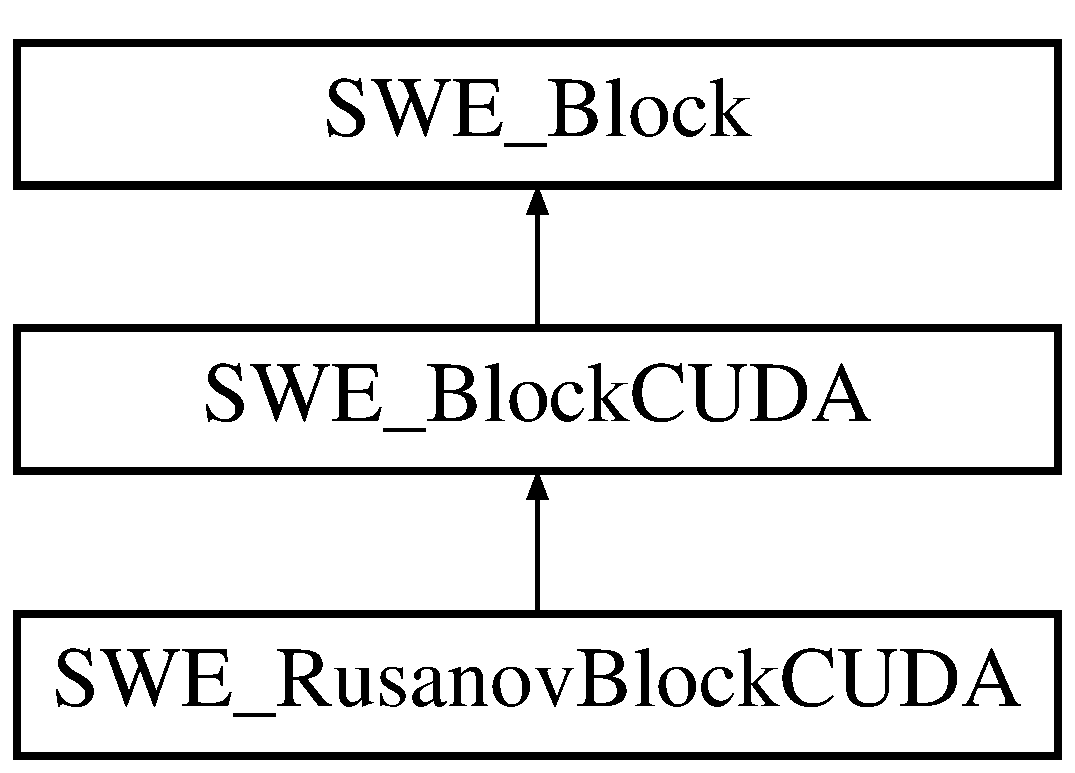
\includegraphics[height=3.000000cm]{classSWE__RusanovBlockCUDA}
\end{center}
\end{figure}
\subsection*{Public Member Functions}
\begin{DoxyCompactItemize}
\item 
\hyperlink{classSWE__RusanovBlockCUDA_a5bd6db4a52d816534923d851ea6f9314}{S\-W\-E\-\_\-\-Rusanov\-Block\-C\-U\-D\-A} (float \-\_\-offset\-X=0, float \-\_\-offset\-Y=0, const int i\-\_\-cuda\-Device=0)
\item 
virtual \hyperlink{classSWE__RusanovBlockCUDA_a4af9183cc7715e1b1a3d91cdb98f9cda}{$\sim$\-S\-W\-E\-\_\-\-Rusanov\-Block\-C\-U\-D\-A} ()
\item 
virtual void \hyperlink{classSWE__RusanovBlockCUDA_a85ec49606ab69ded8cd6f39aa4be1505}{compute\-Numerical\-Fluxes} ()
\item 
virtual void \hyperlink{classSWE__RusanovBlockCUDA_a0a18726a733492218423eed37a7ab406}{update\-Unknowns} (float dt)
\item 
virtual void \hyperlink{classSWE__RusanovBlockCUDA_a238b383e0458babb52e3dd5b5784bc48}{simulate\-Timestep} (float dt)
\begin{DoxyCompactList}\small\item\em execute a single time step of the simulation \end{DoxyCompactList}\item 
virtual float \hyperlink{classSWE__RusanovBlockCUDA_a77719262dc1789adea136ed50f17bb58}{simulate} (float t\-Start, float t\-End)
\end{DoxyCompactItemize}
\subsection*{Friends}
\begin{DoxyCompactItemize}
\item 
ostream \& \hyperlink{classSWE__RusanovBlockCUDA_adbdcb6417643b695657724ea16f84954}{operator$<$$<$} (ostream \&os, const \hyperlink{classSWE__RusanovBlockCUDA}{S\-W\-E\-\_\-\-Rusanov\-Block\-C\-U\-D\-A} \&swe)
\end{DoxyCompactItemize}
\subsection*{Additional Inherited Members}


\subsection{Detailed Description}
\hyperlink{classSWE__RusanovBlockCUDA}{S\-W\-E\-\_\-\-Rusanov\-Block\-C\-U\-D\-A} extends the base class \hyperlink{classSWE__BlockCUDA}{S\-W\-E\-\_\-\-Block\-C\-U\-D\-A}, and provides a concrete C\-U\-D\-A implementation of a simple shallow water model based on Rusanov Flux computation on the edges and explicit time stepping. 

\subsection{Constructor \& Destructor Documentation}
\hypertarget{classSWE__RusanovBlockCUDA_a5bd6db4a52d816534923d851ea6f9314}{\index{S\-W\-E\-\_\-\-Rusanov\-Block\-C\-U\-D\-A@{S\-W\-E\-\_\-\-Rusanov\-Block\-C\-U\-D\-A}!S\-W\-E\-\_\-\-Rusanov\-Block\-C\-U\-D\-A@{S\-W\-E\-\_\-\-Rusanov\-Block\-C\-U\-D\-A}}
\index{S\-W\-E\-\_\-\-Rusanov\-Block\-C\-U\-D\-A@{S\-W\-E\-\_\-\-Rusanov\-Block\-C\-U\-D\-A}!SWE_RusanovBlockCUDA@{S\-W\-E\-\_\-\-Rusanov\-Block\-C\-U\-D\-A}}
\subsubsection[{S\-W\-E\-\_\-\-Rusanov\-Block\-C\-U\-D\-A}]{\setlength{\rightskip}{0pt plus 5cm}S\-W\-E\-\_\-\-Rusanov\-Block\-C\-U\-D\-A\-::\-S\-W\-E\-\_\-\-Rusanov\-Block\-C\-U\-D\-A (
\begin{DoxyParamCaption}
\item[{float}]{\-\_\-offset\-X = {\ttfamily 0}, }
\item[{float}]{\-\_\-offset\-Y = {\ttfamily 0}, }
\item[{const int}]{i\-\_\-cuda\-Device = {\ttfamily 0}}
\end{DoxyParamCaption}
)}}\label{classSWE__RusanovBlockCUDA_a5bd6db4a52d816534923d851ea6f9314}
Constructor\-: allocate variables for simulation

unknowns h,hu,hv,b are defined on grid indices \mbox{[}0,..,nx+1\mbox{]}$\ast$\mbox{[}0,..,ny+1\mbox{]} -\/$>$ computational domain is \mbox{[}1,..,nx\mbox{]}$\ast$\mbox{[}1,..,ny\mbox{]} -\/$>$ plus ghost cell layer

flux terms are defined for edges with indices \mbox{[}0,..,nx\mbox{]}$\ast$\mbox{[}1,..,ny\mbox{]} or \mbox{[}1,..,nx\mbox{]}$\ast$\href{for horizontal/vertical edges}{\tt 0,..,ny} Flux term with index (i,j) is located on the edge between cells with index (i,j) and (i+1,j) or (i,j+1)

bathymetry source terms are defined for cells with indices \mbox{[}1,..,nx\mbox{]}$\ast$\mbox{[}1,..,ny\mbox{]} \hypertarget{classSWE__RusanovBlockCUDA_a4af9183cc7715e1b1a3d91cdb98f9cda}{\index{S\-W\-E\-\_\-\-Rusanov\-Block\-C\-U\-D\-A@{S\-W\-E\-\_\-\-Rusanov\-Block\-C\-U\-D\-A}!$\sim$\-S\-W\-E\-\_\-\-Rusanov\-Block\-C\-U\-D\-A@{$\sim$\-S\-W\-E\-\_\-\-Rusanov\-Block\-C\-U\-D\-A}}
\index{$\sim$\-S\-W\-E\-\_\-\-Rusanov\-Block\-C\-U\-D\-A@{$\sim$\-S\-W\-E\-\_\-\-Rusanov\-Block\-C\-U\-D\-A}!SWE_RusanovBlockCUDA@{S\-W\-E\-\_\-\-Rusanov\-Block\-C\-U\-D\-A}}
\subsubsection[{$\sim$\-S\-W\-E\-\_\-\-Rusanov\-Block\-C\-U\-D\-A}]{\setlength{\rightskip}{0pt plus 5cm}S\-W\-E\-\_\-\-Rusanov\-Block\-C\-U\-D\-A\-::$\sim$\-S\-W\-E\-\_\-\-Rusanov\-Block\-C\-U\-D\-A (
\begin{DoxyParamCaption}
{}
\end{DoxyParamCaption}
)\hspace{0.3cm}{\ttfamily [virtual]}}}\label{classSWE__RusanovBlockCUDA_a4af9183cc7715e1b1a3d91cdb98f9cda}
Destructor\-: de-\/allocate all variables 

\subsection{Member Function Documentation}
\hypertarget{classSWE__RusanovBlockCUDA_a85ec49606ab69ded8cd6f39aa4be1505}{\index{S\-W\-E\-\_\-\-Rusanov\-Block\-C\-U\-D\-A@{S\-W\-E\-\_\-\-Rusanov\-Block\-C\-U\-D\-A}!compute\-Numerical\-Fluxes@{compute\-Numerical\-Fluxes}}
\index{compute\-Numerical\-Fluxes@{compute\-Numerical\-Fluxes}!SWE_RusanovBlockCUDA@{S\-W\-E\-\_\-\-Rusanov\-Block\-C\-U\-D\-A}}
\subsubsection[{compute\-Numerical\-Fluxes}]{\setlength{\rightskip}{0pt plus 5cm}void S\-W\-E\-\_\-\-Rusanov\-Block\-C\-U\-D\-A\-::compute\-Numerical\-Fluxes (
\begin{DoxyParamCaption}
{}
\end{DoxyParamCaption}
)\hspace{0.3cm}{\ttfamily [virtual]}}}\label{classSWE__RusanovBlockCUDA_a85ec49606ab69ded8cd6f39aa4be1505}
compute the flux terms on all edges 

Implements \hyperlink{classSWE__Block_a94dcf2c6ae31731e4586e45628b0c00e}{S\-W\-E\-\_\-\-Block}.

\hypertarget{classSWE__RusanovBlockCUDA_a77719262dc1789adea136ed50f17bb58}{\index{S\-W\-E\-\_\-\-Rusanov\-Block\-C\-U\-D\-A@{S\-W\-E\-\_\-\-Rusanov\-Block\-C\-U\-D\-A}!simulate@{simulate}}
\index{simulate@{simulate}!SWE_RusanovBlockCUDA@{S\-W\-E\-\_\-\-Rusanov\-Block\-C\-U\-D\-A}}
\subsubsection[{simulate}]{\setlength{\rightskip}{0pt plus 5cm}\-\_\-\-\_\-host\-\_\-\-\_\- float S\-W\-E\-\_\-\-Rusanov\-Block\-C\-U\-D\-A\-::simulate (
\begin{DoxyParamCaption}
\item[{float}]{t\-Start, }
\item[{float}]{t\-End}
\end{DoxyParamCaption}
)\hspace{0.3cm}{\ttfamily [virtual]}}}\label{classSWE__RusanovBlockCUDA_a77719262dc1789adea136ed50f17bb58}
perform forward-\/\-Euler time steps, starting with simulation time t\-Start,\-: until simulation time t\-End is reached; device-\/global variables hd, hud, hvd are updated; unknowns h, hu, hv in main memory are not updated. Ghost layers and bathymetry sources are updated between timesteps. intended as main simulation loop between two checkpoints 

Reimplemented from \hyperlink{classSWE__Block_a69784e2be2d09035fb2af9d306768f07}{S\-W\-E\-\_\-\-Block}.

\hypertarget{classSWE__RusanovBlockCUDA_a238b383e0458babb52e3dd5b5784bc48}{\index{S\-W\-E\-\_\-\-Rusanov\-Block\-C\-U\-D\-A@{S\-W\-E\-\_\-\-Rusanov\-Block\-C\-U\-D\-A}!simulate\-Timestep@{simulate\-Timestep}}
\index{simulate\-Timestep@{simulate\-Timestep}!SWE_RusanovBlockCUDA@{S\-W\-E\-\_\-\-Rusanov\-Block\-C\-U\-D\-A}}
\subsubsection[{simulate\-Timestep}]{\setlength{\rightskip}{0pt plus 5cm}void S\-W\-E\-\_\-\-Rusanov\-Block\-C\-U\-D\-A\-::simulate\-Timestep (
\begin{DoxyParamCaption}
\item[{float}]{dt}
\end{DoxyParamCaption}
)\hspace{0.3cm}{\ttfamily [virtual]}}}\label{classSWE__RusanovBlockCUDA_a238b383e0458babb52e3dd5b5784bc48}


execute a single time step of the simulation 

Depending on the current values of h, hu, hv (incl. ghost layers) update these unknowns in each grid cell (ghost layers and bathymetry are not updated). The Rusanov C\-U\-D\-A-\/implementation of simulate\-Timestep subsequently calls the functions compute\-Numerical\-Fluxes (to compute all fluxes on grid edges), and update\-Unknowns (to update the variables according to flux values, typically according to an Euler time step). 
\begin{DoxyParams}{Parameters}
{\em dt} & size of the time step \\
\hline
\end{DoxyParams}


Reimplemented from \hyperlink{classSWE__Block_add6908e1ceb261a0a1f3ebc262cc5f11}{S\-W\-E\-\_\-\-Block}.

\hypertarget{classSWE__RusanovBlockCUDA_a0a18726a733492218423eed37a7ab406}{\index{S\-W\-E\-\_\-\-Rusanov\-Block\-C\-U\-D\-A@{S\-W\-E\-\_\-\-Rusanov\-Block\-C\-U\-D\-A}!update\-Unknowns@{update\-Unknowns}}
\index{update\-Unknowns@{update\-Unknowns}!SWE_RusanovBlockCUDA@{S\-W\-E\-\_\-\-Rusanov\-Block\-C\-U\-D\-A}}
\subsubsection[{update\-Unknowns}]{\setlength{\rightskip}{0pt plus 5cm}\-\_\-\-\_\-host\-\_\-\-\_\- void S\-W\-E\-\_\-\-Rusanov\-Block\-C\-U\-D\-A\-::update\-Unknowns (
\begin{DoxyParamCaption}
\item[{float}]{dt}
\end{DoxyParamCaption}
)\hspace{0.3cm}{\ttfamily [virtual]}}}\label{classSWE__RusanovBlockCUDA_a0a18726a733492218423eed37a7ab406}
implements interface function update\-Unknowns\-: based on the (Rusanov) fluxes computed on each edge (and stored in the variables Fh, Gh, etc.); compute the balance terms for each cell, and update the unknowns according to an Euler time step. It will force an update of the copy layer in the main memory by calling \hyperlink{classSWE__BlockCUDA_a41d117ca8fe9a8c5509369edd026fd63}{synch\-Copy\-Layer\-Before\-Read()}, and provide an compute the maximum allowed time step size by calling compute\-Max\-Timestep\-C\-U\-D\-A(). 
\begin{DoxyParams}{Parameters}
{\em dt} & size of the time step. \\
\hline
\end{DoxyParams}


Implements \hyperlink{classSWE__Block_ab2b4b659f23d5d45413dece8d2da3298}{S\-W\-E\-\_\-\-Block}.



\subsection{Friends And Related Function Documentation}
\hypertarget{classSWE__RusanovBlockCUDA_adbdcb6417643b695657724ea16f84954}{\index{S\-W\-E\-\_\-\-Rusanov\-Block\-C\-U\-D\-A@{S\-W\-E\-\_\-\-Rusanov\-Block\-C\-U\-D\-A}!operator$<$$<$@{operator$<$$<$}}
\index{operator$<$$<$@{operator$<$$<$}!SWE_RusanovBlockCUDA@{S\-W\-E\-\_\-\-Rusanov\-Block\-C\-U\-D\-A}}
\subsubsection[{operator$<$$<$}]{\setlength{\rightskip}{0pt plus 5cm}ostream\& operator$<$$<$ (
\begin{DoxyParamCaption}
\item[{ostream \&}]{os, }
\item[{const {\bf S\-W\-E\-\_\-\-Rusanov\-Block\-C\-U\-D\-A} \&}]{swe}
\end{DoxyParamCaption}
)\hspace{0.3cm}{\ttfamily [friend]}}}\label{classSWE__RusanovBlockCUDA_adbdcb6417643b695657724ea16f84954}
overload operator$<$$<$ such that data can be written via cout $<$$<$ -\/$>$ needs to be declared as friend to be allowed to access private data 

The documentation for this class was generated from the following files\-:\begin{DoxyCompactItemize}
\item 
/home/sascha/\-Dokumente/\-Projects/\-Tsun\-Sim/\-S\-W\-E/src/blocks/rusanov/\hyperlink{SWE__RusanovBlockCUDA_8hh}{S\-W\-E\-\_\-\-Rusanov\-Block\-C\-U\-D\-A.\-hh}\item 
/home/sascha/\-Dokumente/\-Projects/\-Tsun\-Sim/\-S\-W\-E/src/blocks/rusanov/\hyperlink{SWE__RusanovBlockCUDA_8cu}{S\-W\-E\-\_\-\-Rusanov\-Block\-C\-U\-D\-A.\-cu}\end{DoxyCompactItemize}

\hypertarget{classSWE__Scenario}{\section{S\-W\-E\-\_\-\-Scenario Class Reference}
\label{classSWE__Scenario}\index{S\-W\-E\-\_\-\-Scenario@{S\-W\-E\-\_\-\-Scenario}}
}


{\ttfamily \#include $<$S\-W\-E\-\_\-\-Scenario.\-hh$>$}

Inheritance diagram for S\-W\-E\-\_\-\-Scenario\-:\begin{figure}[H]
\begin{center}
\leavevmode
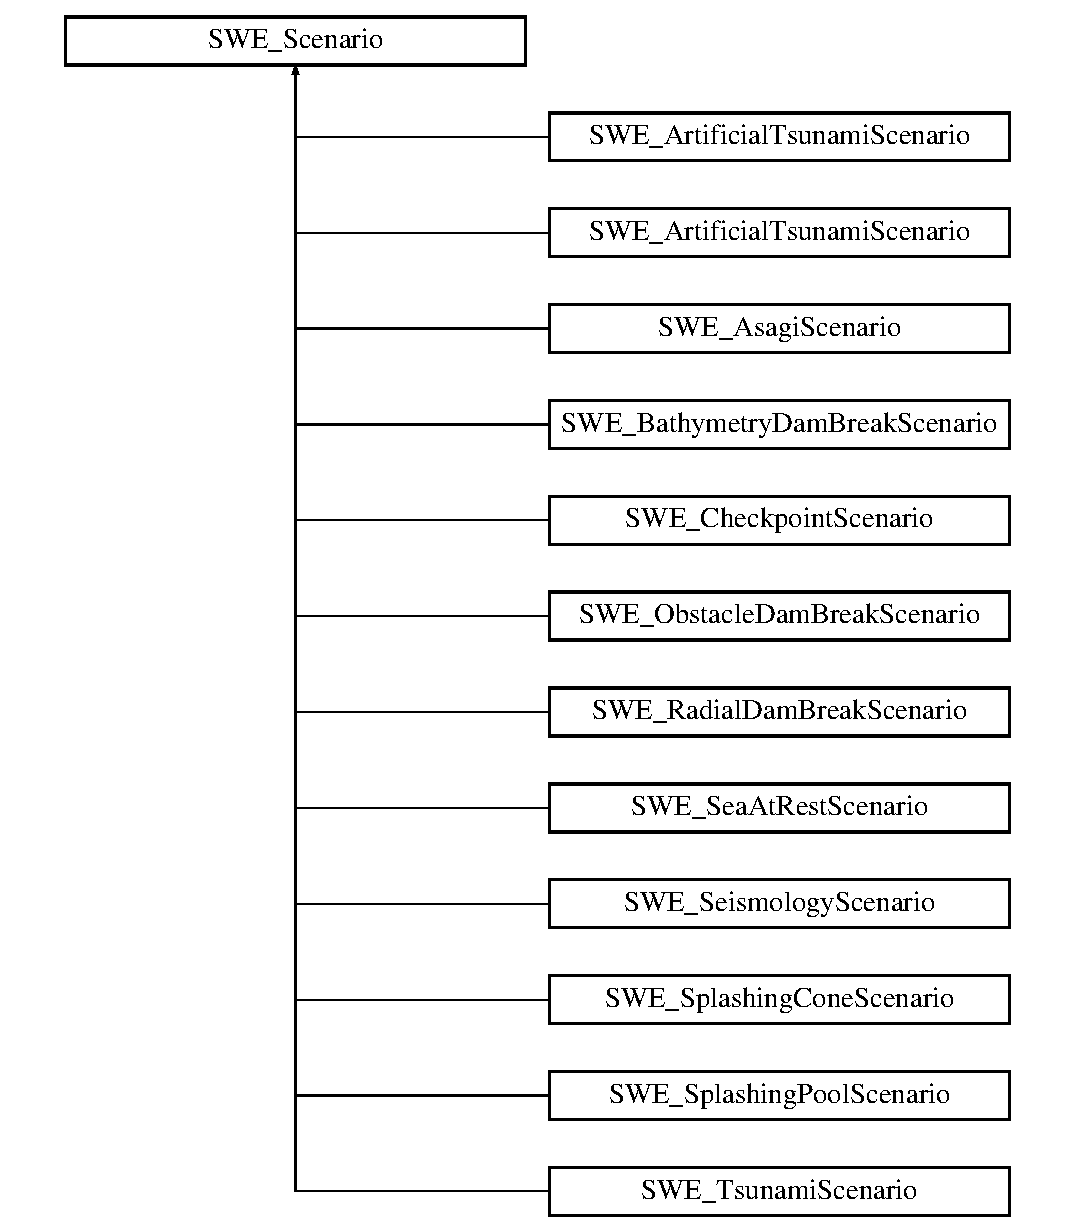
\includegraphics[height=11.000000cm]{classSWE__Scenario}
\end{center}
\end{figure}
\subsection*{Public Member Functions}
\begin{DoxyCompactItemize}
\item 
\hypertarget{classSWE__Scenario_a8b7fa4a4a64128d4f37330bb1ff6b26a}{{\bfseries S\-W\-E\-\_\-\-Scenario} (int x, int y, \hyperlink{SWE__Scenario_8hh_af75d5dd7322fa39ed0af4e7839e600f8}{Boundary\-Type} bounds=W\-A\-L\-L)}\label{classSWE__Scenario_a8b7fa4a4a64128d4f37330bb1ff6b26a}

\item 
\hypertarget{classSWE__Scenario_ade6f356d60b1402c034611266462b88b}{virtual float {\bfseries get\-Water\-Height} (float x, float y)}\label{classSWE__Scenario_ade6f356d60b1402c034611266462b88b}

\item 
\hypertarget{classSWE__Scenario_ab1d5e360c861df3c8c0ccd919bd7f495}{virtual float {\bfseries get\-Veloc\-\_\-u} (float x, float y)}\label{classSWE__Scenario_ab1d5e360c861df3c8c0ccd919bd7f495}

\item 
\hypertarget{classSWE__Scenario_afeaf75872a1678ea64e6f7accd1e49c6}{virtual float {\bfseries get\-Veloc\-\_\-v} (float x, float y)}\label{classSWE__Scenario_afeaf75872a1678ea64e6f7accd1e49c6}

\item 
\hypertarget{classSWE__Scenario_afe09a1ba63304800651f25873570a348}{virtual float {\bfseries get\-Bathymetry} (float x, float y)}\label{classSWE__Scenario_afe09a1ba63304800651f25873570a348}

\item 
\hypertarget{classSWE__Scenario_a86f33e15398c7e3de715c4d80e719e7e}{virtual int {\bfseries get\-Cells\-X} ()}\label{classSWE__Scenario_a86f33e15398c7e3de715c4d80e719e7e}

\item 
\hypertarget{classSWE__Scenario_abf002b0277bff080b82583b6012c2632}{virtual int {\bfseries get\-Cells\-Y} ()}\label{classSWE__Scenario_abf002b0277bff080b82583b6012c2632}

\item 
\hypertarget{classSWE__Scenario_a9de0f0f9fcc34dfe00c522b10c343d91}{virtual float {\bfseries water\-Height\-At\-Rest} ()}\label{classSWE__Scenario_a9de0f0f9fcc34dfe00c522b10c343d91}

\item 
\hypertarget{classSWE__Scenario_a7c4d192d17691191acdde72170d53b7f}{virtual float {\bfseries get\-Last\-Time} ()}\label{classSWE__Scenario_a7c4d192d17691191acdde72170d53b7f}

\item 
\hypertarget{classSWE__Scenario_ae7ed72f584069e9885c33c4ca83f3ff5}{virtual float {\bfseries end\-Simulation} ()}\label{classSWE__Scenario_ae7ed72f584069e9885c33c4ca83f3ff5}

\item 
\hypertarget{classSWE__Scenario_a0c36b8d2bc8d1fc42af68309f958817a}{virtual size\-\_\-t {\bfseries get\-Checkpoint\-Count} ()}\label{classSWE__Scenario_a0c36b8d2bc8d1fc42af68309f958817a}

\item 
\hypertarget{classSWE__Scenario_ab8fe7ce15d7758fb0c4e0e3887b34a5d}{virtual \hyperlink{SWE__Scenario_8hh_af75d5dd7322fa39ed0af4e7839e600f8}{Boundary\-Type} {\bfseries get\-Boundary\-Type} (\hyperlink{SWE__Scenario_8hh_aa5e01e3f7df312f7b9b0d02521141fcc}{Boundary\-Edge} edge)}\label{classSWE__Scenario_ab8fe7ce15d7758fb0c4e0e3887b34a5d}

\item 
\hypertarget{classSWE__Scenario_aef7a53a5d791bee0545488735381c6a2}{void {\bfseries set\-Boundary\-Types} (\hyperlink{SWE__Scenario_8hh_af75d5dd7322fa39ed0af4e7839e600f8}{Boundary\-Type} type)}\label{classSWE__Scenario_aef7a53a5d791bee0545488735381c6a2}

\item 
\hypertarget{classSWE__Scenario_a1b01e953c2079b64f527c9bc5a0c86d7}{virtual float {\bfseries get\-Boundary\-Pos} (\hyperlink{SWE__Scenario_8hh_aa5e01e3f7df312f7b9b0d02521141fcc}{Boundary\-Edge} edge)}\label{classSWE__Scenario_a1b01e953c2079b64f527c9bc5a0c86d7}

\end{DoxyCompactItemize}
\subsection*{Protected Attributes}
\begin{DoxyCompactItemize}
\item 
\hypertarget{classSWE__Scenario_abe1a2cbf009889f9330091b9d28833f0}{\hyperlink{SWE__Scenario_8hh_af75d5dd7322fa39ed0af4e7839e600f8}{Boundary\-Type} {\bfseries bound\-Type}}\label{classSWE__Scenario_abe1a2cbf009889f9330091b9d28833f0}

\item 
\hypertarget{classSWE__Scenario_afa6dda8b7b69dc1514b26b8de5fa321b}{int {\bfseries cells\-\_\-x}}\label{classSWE__Scenario_afa6dda8b7b69dc1514b26b8de5fa321b}

\item 
\hypertarget{classSWE__Scenario_a4cd13fca6b6ab5290426b55b5dd755ff}{int {\bfseries cells\-\_\-y}}\label{classSWE__Scenario_a4cd13fca6b6ab5290426b55b5dd755ff}

\end{DoxyCompactItemize}


\subsection{Detailed Description}
\hyperlink{classSWE__Scenario}{S\-W\-E\-\_\-\-Scenario} defines an interface to initialise the unknowns of a shallow water simulation -\/ i.\-e. to initialise water height, velocities, and bathymatry according to certain scenarios. \hyperlink{classSWE__Scenario}{S\-W\-E\-\_\-\-Scenario} can act as stand-\/alone scenario class, providing a very basic scenario (all functions are constant); however, the idea is to provide derived classes that implement the \hyperlink{classSWE__Scenario}{S\-W\-E\-\_\-\-Scenario} interface for more interesting scenarios. 

The documentation for this class was generated from the following file\-:\begin{DoxyCompactItemize}
\item 
/home/sascha/\-Dokumente/\-Projects/\-Tsun\-Sim/\-S\-W\-E/src/scenarios/\hyperlink{SWE__Scenario_8hh}{S\-W\-E\-\_\-\-Scenario.\-hh}\end{DoxyCompactItemize}

\hypertarget{classSWE__SeaAtRestScenario}{\section{S\-W\-E\-\_\-\-Sea\-At\-Rest\-Scenario Class Reference}
\label{classSWE__SeaAtRestScenario}\index{S\-W\-E\-\_\-\-Sea\-At\-Rest\-Scenario@{S\-W\-E\-\_\-\-Sea\-At\-Rest\-Scenario}}
}


{\ttfamily \#include $<$S\-W\-E\-\_\-simple\-\_\-scenarios.\-hh$>$}

Inheritance diagram for S\-W\-E\-\_\-\-Sea\-At\-Rest\-Scenario\-:\begin{figure}[H]
\begin{center}
\leavevmode
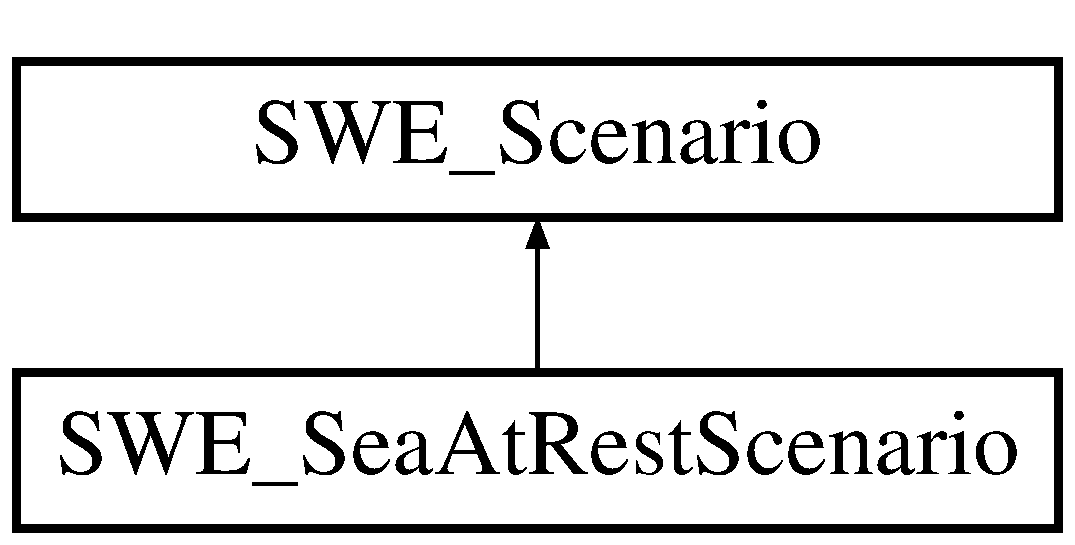
\includegraphics[height=2.000000cm]{classSWE__SeaAtRestScenario}
\end{center}
\end{figure}
\subsection*{Public Member Functions}
\begin{DoxyCompactItemize}
\item 
\hypertarget{classSWE__SeaAtRestScenario_a0d493a2c96cde62cc71035c5f62717d1}{float {\bfseries get\-Water\-Height} (float x, float y)}\label{classSWE__SeaAtRestScenario_a0d493a2c96cde62cc71035c5f62717d1}

\item 
\hypertarget{classSWE__SeaAtRestScenario_a738776f758bb5b914ede2e6f57cb3ffd}{float {\bfseries get\-Bathymetry} (float x, float y)}\label{classSWE__SeaAtRestScenario_a738776f758bb5b914ede2e6f57cb3ffd}

\end{DoxyCompactItemize}


\subsection{Detailed Description}
Scenario \char`\"{}\-Sea at Rest\char`\"{}\-: flat water surface (\char`\"{}sea at rest\char`\"{}), but non-\/uniform bathymetry (id. to \char`\"{}\-Bathymetry Dam Break\char`\"{}) test scenario for \char`\"{}sea at rest\char`\"{}-\/solution 

The documentation for this class was generated from the following file\-:\begin{DoxyCompactItemize}
\item 
/home/sascha/\-Dokumente/\-Projects/\-Tsun\-Sim/\-S\-W\-E/src/scenarios/\hyperlink{SWE__simple__scenarios_8hh}{S\-W\-E\-\_\-simple\-\_\-scenarios.\-hh}\end{DoxyCompactItemize}

\hypertarget{classSWE__SplashingConeScenario}{\section{S\-W\-E\-\_\-\-Splashing\-Cone\-Scenario Class Reference}
\label{classSWE__SplashingConeScenario}\index{S\-W\-E\-\_\-\-Splashing\-Cone\-Scenario@{S\-W\-E\-\_\-\-Splashing\-Cone\-Scenario}}
}


{\ttfamily \#include $<$S\-W\-E\-\_\-simple\-\_\-scenarios.\-hh$>$}

Inheritance diagram for S\-W\-E\-\_\-\-Splashing\-Cone\-Scenario\-:\begin{figure}[H]
\begin{center}
\leavevmode
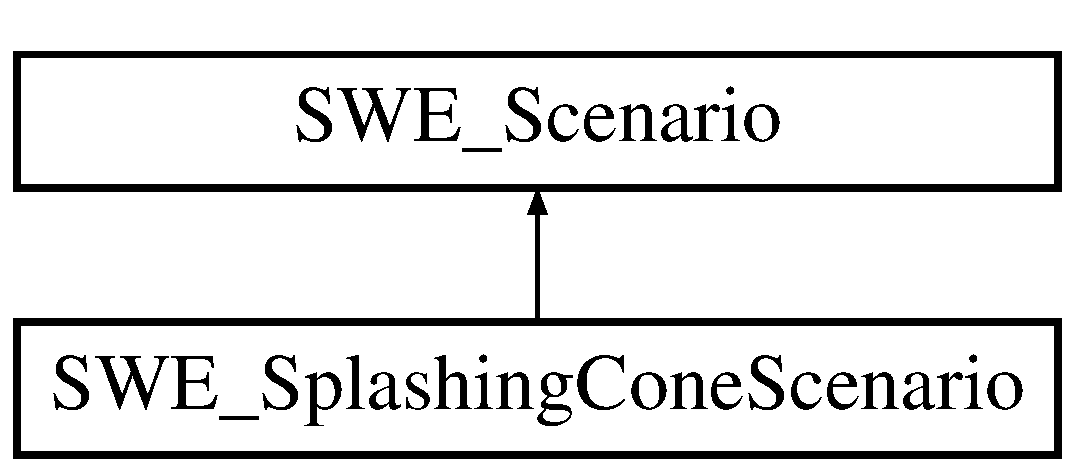
\includegraphics[height=2.000000cm]{classSWE__SplashingConeScenario}
\end{center}
\end{figure}
\subsection*{Public Member Functions}
\begin{DoxyCompactItemize}
\item 
\hypertarget{classSWE__SplashingConeScenario_a63d7b91dbd7dce764b12ba76eae856b9}{float {\bfseries get\-Water\-Height} (float x, float y)}\label{classSWE__SplashingConeScenario_a63d7b91dbd7dce764b12ba76eae856b9}

\item 
\hypertarget{classSWE__SplashingConeScenario_a54dff1212b8261e89270f9ab10081cb1}{float {\bfseries get\-Bathymetry} (float x, float y)}\label{classSWE__SplashingConeScenario_a54dff1212b8261e89270f9ab10081cb1}

\item 
\hypertarget{classSWE__SplashingConeScenario_a430b3220b49368a4d20b69d71c087604}{float {\bfseries water\-Height\-At\-Rest} ()}\label{classSWE__SplashingConeScenario_a430b3220b49368a4d20b69d71c087604}

\item 
\hypertarget{classSWE__SplashingConeScenario_a464b296fc1905efc2e86aba909cc5188}{float {\bfseries end\-Simulation} ()}\label{classSWE__SplashingConeScenario_a464b296fc1905efc2e86aba909cc5188}

\item 
\hypertarget{classSWE__SplashingConeScenario_a8b8353a1f1cd58d9f211ccb32e4f3b33}{virtual \hyperlink{SWE__Scenario_8hh_af75d5dd7322fa39ed0af4e7839e600f8}{Boundary\-Type} {\bfseries get\-Boundary\-Type} (\hyperlink{SWE__Scenario_8hh_aa5e01e3f7df312f7b9b0d02521141fcc}{Boundary\-Edge} edge)}\label{classSWE__SplashingConeScenario_a8b8353a1f1cd58d9f211ccb32e4f3b33}

\end{DoxyCompactItemize}


\subsection{Detailed Description}
Scenario \char`\"{}\-Splashing Cone\char`\"{}\-: bathymetry forms a circular cone intial water surface designed to form \char`\"{}sea at rest\char`\"{} but\-: elevated water region in the centre (similar to radial dam break) 

The documentation for this class was generated from the following file\-:\begin{DoxyCompactItemize}
\item 
/home/sascha/\-Dokumente/\-Projects/\-Tsun\-Sim/\-S\-W\-E/src/scenarios/\hyperlink{SWE__simple__scenarios_8hh}{S\-W\-E\-\_\-simple\-\_\-scenarios.\-hh}\end{DoxyCompactItemize}

\hypertarget{classSWE__SplashingPoolScenario}{\section{S\-W\-E\-\_\-\-Splashing\-Pool\-Scenario Class Reference}
\label{classSWE__SplashingPoolScenario}\index{S\-W\-E\-\_\-\-Splashing\-Pool\-Scenario@{S\-W\-E\-\_\-\-Splashing\-Pool\-Scenario}}
}


{\ttfamily \#include $<$S\-W\-E\-\_\-simple\-\_\-scenarios.\-hh$>$}

Inheritance diagram for S\-W\-E\-\_\-\-Splashing\-Pool\-Scenario\-:\begin{figure}[H]
\begin{center}
\leavevmode
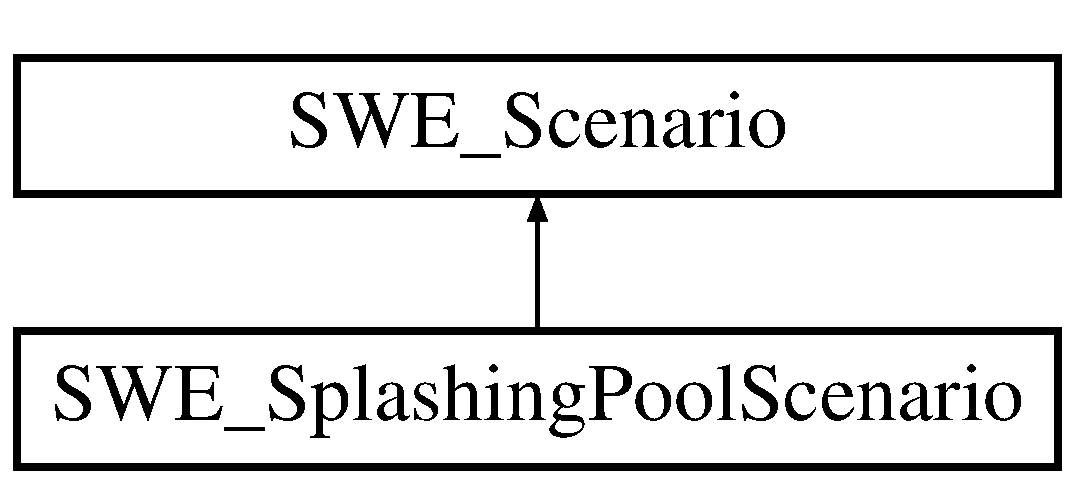
\includegraphics[height=2.000000cm]{classSWE__SplashingPoolScenario}
\end{center}
\end{figure}
\subsection*{Public Member Functions}
\begin{DoxyCompactItemize}
\item 
\hypertarget{classSWE__SplashingPoolScenario_a75c48073eb863d52fe38639ff0834e72}{float {\bfseries get\-Bathymetry} (float x, float y)}\label{classSWE__SplashingPoolScenario_a75c48073eb863d52fe38639ff0834e72}

\item 
\hypertarget{classSWE__SplashingPoolScenario_a45328d2cbff3068f6bde34d92dff0d1c}{float {\bfseries get\-Water\-Height} (float x, float y)}\label{classSWE__SplashingPoolScenario_a45328d2cbff3068f6bde34d92dff0d1c}

\item 
\hypertarget{classSWE__SplashingPoolScenario_a49edaef6fbfad67c12f0ce1942e9f848}{virtual float {\bfseries end\-Simulation} ()}\label{classSWE__SplashingPoolScenario_a49edaef6fbfad67c12f0ce1942e9f848}

\item 
float \hyperlink{classSWE__SplashingPoolScenario_af9ca3bce236a98e2a7ee5165088c8ed6}{get\-Boundary\-Pos} (\hyperlink{SWE__Scenario_8hh_aa5e01e3f7df312f7b9b0d02521141fcc}{Boundary\-Edge} i\-\_\-edge)
\end{DoxyCompactItemize}
\subsection*{Additional Inherited Members}


\subsection{Detailed Description}
Scenario \char`\"{}\-Splashing Pool\char`\"{}\-: intial water surface has a fixed slope (diagonal to x,y) 

\subsection{Member Function Documentation}
\hypertarget{classSWE__SplashingPoolScenario_af9ca3bce236a98e2a7ee5165088c8ed6}{\index{S\-W\-E\-\_\-\-Splashing\-Pool\-Scenario@{S\-W\-E\-\_\-\-Splashing\-Pool\-Scenario}!get\-Boundary\-Pos@{get\-Boundary\-Pos}}
\index{get\-Boundary\-Pos@{get\-Boundary\-Pos}!SWE_SplashingPoolScenario@{S\-W\-E\-\_\-\-Splashing\-Pool\-Scenario}}
\subsubsection[{get\-Boundary\-Pos}]{\setlength{\rightskip}{0pt plus 5cm}float S\-W\-E\-\_\-\-Splashing\-Pool\-Scenario\-::get\-Boundary\-Pos (
\begin{DoxyParamCaption}
\item[{{\bf Boundary\-Edge}}]{i\-\_\-edge}
\end{DoxyParamCaption}
)\hspace{0.3cm}{\ttfamily [inline]}, {\ttfamily [virtual]}}}\label{classSWE__SplashingPoolScenario_af9ca3bce236a98e2a7ee5165088c8ed6}
Get the boundary positions


\begin{DoxyParams}{Parameters}
{\em i\-\_\-edge} & which edge \\
\hline
\end{DoxyParams}
\begin{DoxyReturn}{Returns}
value in the corresponding dimension 
\end{DoxyReturn}


Reimplemented from \hyperlink{classSWE__Scenario}{S\-W\-E\-\_\-\-Scenario}.



The documentation for this class was generated from the following file\-:\begin{DoxyCompactItemize}
\item 
/home/sascha/\-Dokumente/\-Projects/\-Tsun\-Sim/\-S\-W\-E/src/scenarios/\hyperlink{SWE__simple__scenarios_8hh}{S\-W\-E\-\_\-simple\-\_\-scenarios.\-hh}\end{DoxyCompactItemize}

\hypertarget{classSWE__VisInfo}{\section{S\-W\-E\-\_\-\-Vis\-Info Class Reference}
\label{classSWE__VisInfo}\index{S\-W\-E\-\_\-\-Vis\-Info@{S\-W\-E\-\_\-\-Vis\-Info}}
}


{\ttfamily \#include $<$S\-W\-E\-\_\-\-Vis\-Info.\-hh$>$}

Inheritance diagram for S\-W\-E\-\_\-\-Vis\-Info\-:\begin{figure}[H]
\begin{center}
\leavevmode
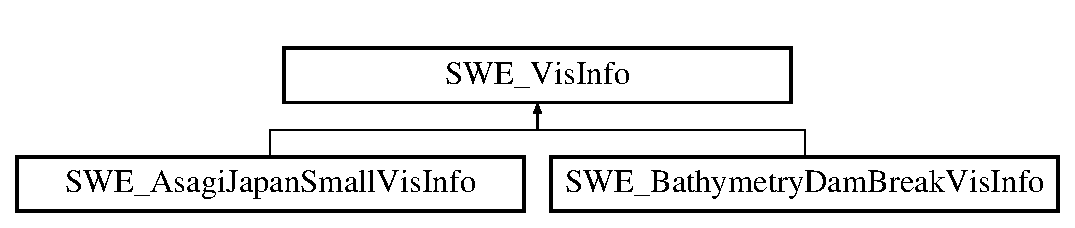
\includegraphics[height=2.000000cm]{classSWE__VisInfo}
\end{center}
\end{figure}
\subsection*{Public Member Functions}
\begin{DoxyCompactItemize}
\item 
virtual \hyperlink{classSWE__VisInfo_a40c49045acf4e50dc29551d767f11e15}{$\sim$\-S\-W\-E\-\_\-\-Vis\-Info} ()
\item 
virtual float \hyperlink{classSWE__VisInfo_a9552a55a7581b7835d415315e2c17f04}{water\-Vertical\-Scaling} ()
\item 
virtual float \hyperlink{classSWE__VisInfo_a9c24e444c209f6f0c03a96950931e677}{bathy\-Vertical\-Offset} ()
\item 
virtual float \hyperlink{classSWE__VisInfo_a10ddd7a192e67c69832e695e48b26e91}{bathy\-Vertical\-Scaling} ()
\end{DoxyCompactItemize}


\subsection{Detailed Description}
\hyperlink{classSWE__VisInfo}{S\-W\-E\-\_\-\-Vis\-Info} defines an interface that can be used for online visualization of a shallow water simulation. In particular, it provides information required for proper scaling of the involved variables.

For water height\-: displayed\-Water\-Height = \hyperlink{classSWE__VisInfo_a9552a55a7581b7835d415315e2c17f04}{water\-Vertical\-Scaling()} $\ast$ simulated\-Water\-Height

For bathymetry\-: displayed\-Batyhmetry = \hyperlink{classSWE__VisInfo_a10ddd7a192e67c69832e695e48b26e91}{bathy\-Vertical\-Scaling()} $\ast$ real\-Bathymetry
\begin{DoxyItemize}
\item \hyperlink{classSWE__VisInfo_a9c24e444c209f6f0c03a96950931e677}{bathy\-Vertical\-Offset()}
\end{DoxyItemize}

The default water height should be 0. In this case a bathymetry value smaller than 0 means water and a value greater than 0 is land. Therefore bathy\-Vertical\-Offset should 0 for all real scenarios.

If you do not not provide an \hyperlink{classSWE__VisInfo}{S\-W\-E\-\_\-\-Vis\-Info} for scenario, (water$\vert$bathy)Vertical\-Scaling will be guessed form the value initial values. bathy\-Vertical\-Offset is always 0 in this case. 

\subsection{Constructor \& Destructor Documentation}
\hypertarget{classSWE__VisInfo_a40c49045acf4e50dc29551d767f11e15}{\index{S\-W\-E\-\_\-\-Vis\-Info@{S\-W\-E\-\_\-\-Vis\-Info}!$\sim$\-S\-W\-E\-\_\-\-Vis\-Info@{$\sim$\-S\-W\-E\-\_\-\-Vis\-Info}}
\index{$\sim$\-S\-W\-E\-\_\-\-Vis\-Info@{$\sim$\-S\-W\-E\-\_\-\-Vis\-Info}!SWE_VisInfo@{S\-W\-E\-\_\-\-Vis\-Info}}
\subsubsection[{$\sim$\-S\-W\-E\-\_\-\-Vis\-Info}]{\setlength{\rightskip}{0pt plus 5cm}virtual S\-W\-E\-\_\-\-Vis\-Info\-::$\sim$\-S\-W\-E\-\_\-\-Vis\-Info (
\begin{DoxyParamCaption}
{}
\end{DoxyParamCaption}
)\hspace{0.3cm}{\ttfamily [inline]}, {\ttfamily [virtual]}}}\label{classSWE__VisInfo_a40c49045acf4e50dc29551d767f11e15}
Empty virtual destructor 

\subsection{Member Function Documentation}
\hypertarget{classSWE__VisInfo_a9c24e444c209f6f0c03a96950931e677}{\index{S\-W\-E\-\_\-\-Vis\-Info@{S\-W\-E\-\_\-\-Vis\-Info}!bathy\-Vertical\-Offset@{bathy\-Vertical\-Offset}}
\index{bathy\-Vertical\-Offset@{bathy\-Vertical\-Offset}!SWE_VisInfo@{S\-W\-E\-\_\-\-Vis\-Info}}
\subsubsection[{bathy\-Vertical\-Offset}]{\setlength{\rightskip}{0pt plus 5cm}virtual float S\-W\-E\-\_\-\-Vis\-Info\-::bathy\-Vertical\-Offset (
\begin{DoxyParamCaption}
{}
\end{DoxyParamCaption}
)\hspace{0.3cm}{\ttfamily [inline]}, {\ttfamily [virtual]}}}\label{classSWE__VisInfo_a9c24e444c209f6f0c03a96950931e677}
\begin{DoxyReturn}{Returns}
The vertical offset for the bathymetry. Should be 0 for \char`\"{}real\char`\"{} scenarios (scenarios with dry areas) 
\end{DoxyReturn}


Reimplemented in \hyperlink{classSWE__BathymetryDamBreakVisInfo_aaecf007665b780a6066485ea0d2d2695}{S\-W\-E\-\_\-\-Bathymetry\-Dam\-Break\-Vis\-Info}.

\hypertarget{classSWE__VisInfo_a10ddd7a192e67c69832e695e48b26e91}{\index{S\-W\-E\-\_\-\-Vis\-Info@{S\-W\-E\-\_\-\-Vis\-Info}!bathy\-Vertical\-Scaling@{bathy\-Vertical\-Scaling}}
\index{bathy\-Vertical\-Scaling@{bathy\-Vertical\-Scaling}!SWE_VisInfo@{S\-W\-E\-\_\-\-Vis\-Info}}
\subsubsection[{bathy\-Vertical\-Scaling}]{\setlength{\rightskip}{0pt plus 5cm}virtual float S\-W\-E\-\_\-\-Vis\-Info\-::bathy\-Vertical\-Scaling (
\begin{DoxyParamCaption}
{}
\end{DoxyParamCaption}
)\hspace{0.3cm}{\ttfamily [inline]}, {\ttfamily [virtual]}}}\label{classSWE__VisInfo_a10ddd7a192e67c69832e695e48b26e91}
\begin{DoxyReturn}{Returns}
The vertical scaling factor for the bathymetry 
\end{DoxyReturn}


Reimplemented in \hyperlink{classSWE__AsagiJapanSmallVisInfo_ab25d85575460a76d88b90e2c927d49ac}{S\-W\-E\-\_\-\-Asagi\-Japan\-Small\-Vis\-Info}.

\hypertarget{classSWE__VisInfo_a9552a55a7581b7835d415315e2c17f04}{\index{S\-W\-E\-\_\-\-Vis\-Info@{S\-W\-E\-\_\-\-Vis\-Info}!water\-Vertical\-Scaling@{water\-Vertical\-Scaling}}
\index{water\-Vertical\-Scaling@{water\-Vertical\-Scaling}!SWE_VisInfo@{S\-W\-E\-\_\-\-Vis\-Info}}
\subsubsection[{water\-Vertical\-Scaling}]{\setlength{\rightskip}{0pt plus 5cm}virtual float S\-W\-E\-\_\-\-Vis\-Info\-::water\-Vertical\-Scaling (
\begin{DoxyParamCaption}
{}
\end{DoxyParamCaption}
)\hspace{0.3cm}{\ttfamily [inline]}, {\ttfamily [virtual]}}}\label{classSWE__VisInfo_a9552a55a7581b7835d415315e2c17f04}
\begin{DoxyReturn}{Returns}
The vertical scaling factor of the water 
\end{DoxyReturn}


Reimplemented in \hyperlink{classSWE__AsagiJapanSmallVisInfo_a9c2092b5e02596e5ca2ba57c39d3b77e}{S\-W\-E\-\_\-\-Asagi\-Japan\-Small\-Vis\-Info}.



The documentation for this class was generated from the following file\-:\begin{DoxyCompactItemize}
\item 
/home/sascha/\-Dokumente/\-Projects/\-Tsun\-Sim/\-S\-W\-E/src/scenarios/\hyperlink{SWE__VisInfo_8hh}{S\-W\-E\-\_\-\-Vis\-Info.\-hh}\end{DoxyCompactItemize}

\hypertarget{classSWE__WaveAccumulationBlock}{\section{S\-W\-E\-\_\-\-Wave\-Accumulation\-Block Class Reference}
\label{classSWE__WaveAccumulationBlock}\index{S\-W\-E\-\_\-\-Wave\-Accumulation\-Block@{S\-W\-E\-\_\-\-Wave\-Accumulation\-Block}}
}


{\ttfamily \#include $<$S\-W\-E\-\_\-\-Wave\-Accumulation\-Block.\-hh$>$}

Inheritance diagram for S\-W\-E\-\_\-\-Wave\-Accumulation\-Block\-:\begin{figure}[H]
\begin{center}
\leavevmode
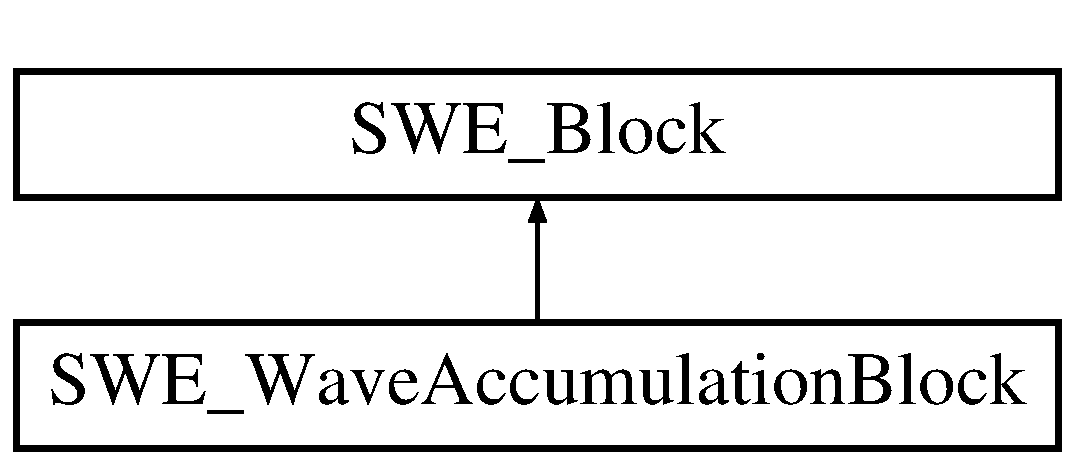
\includegraphics[height=2.000000cm]{classSWE__WaveAccumulationBlock}
\end{center}
\end{figure}
\subsection*{Public Member Functions}
\begin{DoxyCompactItemize}
\item 
\hyperlink{classSWE__WaveAccumulationBlock_a20e04bf219dbf3d82c9f5eac1e7bd848}{S\-W\-E\-\_\-\-Wave\-Accumulation\-Block} (int l\-\_\-nx, int l\-\_\-ny, float l\-\_\-dx, float l\-\_\-dy)
\item 
void \hyperlink{classSWE__WaveAccumulationBlock_acac0b73f22b256bc91a58ff8d0831e5d}{compute\-Numerical\-Fluxes} ()
\item 
void \hyperlink{classSWE__WaveAccumulationBlock_a67b78723e81aec6e661b3710e6c41b43}{update\-Unknowns} (float dt)
\end{DoxyCompactItemize}
\subsection*{Additional Inherited Members}


\subsection{Detailed Description}
\hyperlink{classSWE__WaveAccumulationBlock}{S\-W\-E\-\_\-\-Wave\-Accumulation\-Block} is an implementation of the \hyperlink{classSWE__Block}{S\-W\-E\-\_\-\-Block} abstract class. It uses a wave propagation solver which is defined with the pre-\/compiler flag W\-A\-V\-E\-\_\-\-P\-R\-O\-P\-A\-G\-A\-T\-I\-O\-N\-\_\-\-S\-O\-L\-V\-E\-R (see above).

Possible wave propagation solvers are\-: F-\/\-Wave, Apprximate Augmented Riemann, Hybrid (f-\/wave + augmented). (details can be found in the corresponding source files) 

\subsection{Constructor \& Destructor Documentation}
\hypertarget{classSWE__WaveAccumulationBlock_a20e04bf219dbf3d82c9f5eac1e7bd848}{\index{S\-W\-E\-\_\-\-Wave\-Accumulation\-Block@{S\-W\-E\-\_\-\-Wave\-Accumulation\-Block}!S\-W\-E\-\_\-\-Wave\-Accumulation\-Block@{S\-W\-E\-\_\-\-Wave\-Accumulation\-Block}}
\index{S\-W\-E\-\_\-\-Wave\-Accumulation\-Block@{S\-W\-E\-\_\-\-Wave\-Accumulation\-Block}!SWE_WaveAccumulationBlock@{S\-W\-E\-\_\-\-Wave\-Accumulation\-Block}}
\subsubsection[{S\-W\-E\-\_\-\-Wave\-Accumulation\-Block}]{\setlength{\rightskip}{0pt plus 5cm}S\-W\-E\-\_\-\-Wave\-Accumulation\-Block\-::\-S\-W\-E\-\_\-\-Wave\-Accumulation\-Block (
\begin{DoxyParamCaption}
\item[{int}]{l\-\_\-nx, }
\item[{int}]{l\-\_\-ny, }
\item[{float}]{l\-\_\-dx, }
\item[{float}]{l\-\_\-dy}
\end{DoxyParamCaption}
)}}\label{classSWE__WaveAccumulationBlock_a20e04bf219dbf3d82c9f5eac1e7bd848}
Constructor of a \hyperlink{classSWE__WaveAccumulationBlock}{S\-W\-E\-\_\-\-Wave\-Accumulation\-Block}.

Allocates the variables for the simulation\-: unknowns h,hu,hv,b are defined on grid indices \mbox{[}0,..,nx+1\mbox{]}$\ast$\mbox{[}0,..,ny+1\mbox{]} (-\/$>$ Abstract class \hyperlink{classSWE__Block}{S\-W\-E\-\_\-\-Block}) -\/$>$ computational domain is \mbox{[}1,..,nx\mbox{]}$\ast$\mbox{[}1,..,ny\mbox{]} -\/$>$ plus ghost cell layer

Similar, all net-\/updates are defined as cell-\/local variables with indices \mbox{[}0,..,nx+1\mbox{]}$\ast$\mbox{[}0,..,ny+1\mbox{]}, however, only values on \mbox{[}1,..,nx\mbox{]}$\ast$\mbox{[}1,..,ny\mbox{]} are used (i.\-e., ghost layers are not accessed). Net updates are intended to hold the accumulated(!) net updates computed on the edges. 

\subsection{Member Function Documentation}
\hypertarget{classSWE__WaveAccumulationBlock_acac0b73f22b256bc91a58ff8d0831e5d}{\index{S\-W\-E\-\_\-\-Wave\-Accumulation\-Block@{S\-W\-E\-\_\-\-Wave\-Accumulation\-Block}!compute\-Numerical\-Fluxes@{compute\-Numerical\-Fluxes}}
\index{compute\-Numerical\-Fluxes@{compute\-Numerical\-Fluxes}!SWE_WaveAccumulationBlock@{S\-W\-E\-\_\-\-Wave\-Accumulation\-Block}}
\subsubsection[{compute\-Numerical\-Fluxes}]{\setlength{\rightskip}{0pt plus 5cm}void S\-W\-E\-\_\-\-Wave\-Accumulation\-Block\-::compute\-Numerical\-Fluxes (
\begin{DoxyParamCaption}
{}
\end{DoxyParamCaption}
)\hspace{0.3cm}{\ttfamily [virtual]}}}\label{classSWE__WaveAccumulationBlock_acac0b73f22b256bc91a58ff8d0831e5d}
Compute net updates for the block. The member variable \hyperlink{classSWE__Block_a05cbc9b40e0483bf73dbc2bdeae7dee3}{max\-Timestep} will be updated with the maximum allowed time step size 

Implements \hyperlink{classSWE__Block_a94dcf2c6ae31731e4586e45628b0c00e}{S\-W\-E\-\_\-\-Block}.

\hypertarget{classSWE__WaveAccumulationBlock_a67b78723e81aec6e661b3710e6c41b43}{\index{S\-W\-E\-\_\-\-Wave\-Accumulation\-Block@{S\-W\-E\-\_\-\-Wave\-Accumulation\-Block}!update\-Unknowns@{update\-Unknowns}}
\index{update\-Unknowns@{update\-Unknowns}!SWE_WaveAccumulationBlock@{S\-W\-E\-\_\-\-Wave\-Accumulation\-Block}}
\subsubsection[{update\-Unknowns}]{\setlength{\rightskip}{0pt plus 5cm}void S\-W\-E\-\_\-\-Wave\-Accumulation\-Block\-::update\-Unknowns (
\begin{DoxyParamCaption}
\item[{float}]{dt}
\end{DoxyParamCaption}
)\hspace{0.3cm}{\ttfamily [virtual]}}}\label{classSWE__WaveAccumulationBlock_a67b78723e81aec6e661b3710e6c41b43}
Updates the unknowns with the already computed net-\/updates.


\begin{DoxyParams}{Parameters}
{\em dt} & time step width used in the update. \\
\hline
\end{DoxyParams}


Implements \hyperlink{classSWE__Block_ab2b4b659f23d5d45413dece8d2da3298}{S\-W\-E\-\_\-\-Block}.



The documentation for this class was generated from the following files\-:\begin{DoxyCompactItemize}
\item 
src/blocks/\hyperlink{SWE__WaveAccumulationBlock_8hh}{S\-W\-E\-\_\-\-Wave\-Accumulation\-Block.\-hh}\item 
src/blocks/\hyperlink{SWE__WaveAccumulationBlock_8cpp}{S\-W\-E\-\_\-\-Wave\-Accumulation\-Block.\-cpp}\end{DoxyCompactItemize}

\hypertarget{classSWE__WavePropagationBlock}{\section{S\-W\-E\-\_\-\-Wave\-Propagation\-Block Class Reference}
\label{classSWE__WavePropagationBlock}\index{S\-W\-E\-\_\-\-Wave\-Propagation\-Block@{S\-W\-E\-\_\-\-Wave\-Propagation\-Block}}
}


{\ttfamily \#include $<$S\-W\-E\-\_\-\-Wave\-Propagation\-Block.\-hh$>$}

Inheritance diagram for S\-W\-E\-\_\-\-Wave\-Propagation\-Block\-:\begin{figure}[H]
\begin{center}
\leavevmode
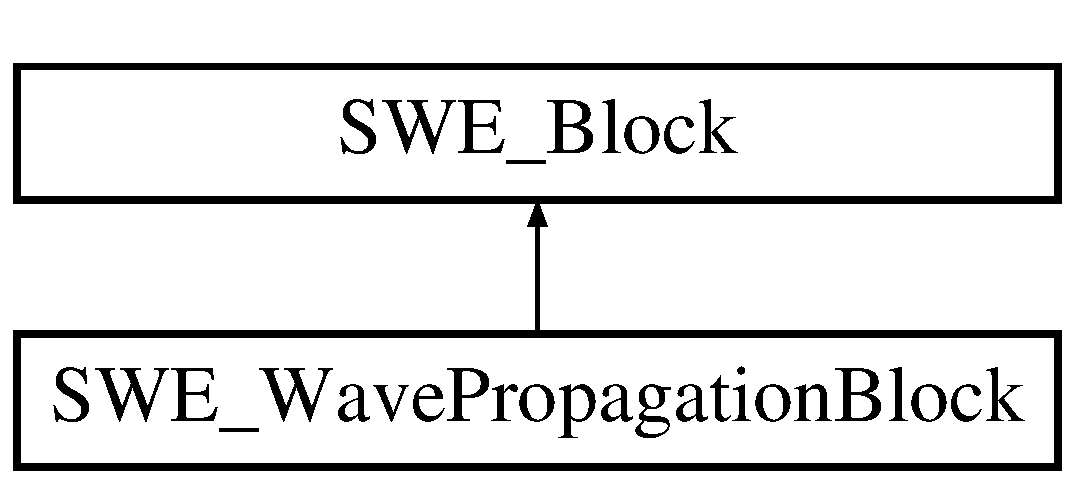
\includegraphics[height=2.000000cm]{classSWE__WavePropagationBlock}
\end{center}
\end{figure}
\subsection*{Public Member Functions}
\begin{DoxyCompactItemize}
\item 
\hyperlink{classSWE__WavePropagationBlock_a9727e083d56a6d7aa9910f50c43080a9}{S\-W\-E\-\_\-\-Wave\-Propagation\-Block} (int l\-\_\-nx, int l\-\_\-ny, float l\-\_\-dx, float l\-\_\-dy)
\item 
void \hyperlink{classSWE__WavePropagationBlock_a5f6335a38fb3cf38623326959f06baf4}{compute\-Numerical\-Fluxes} ()
\item 
void \hyperlink{classSWE__WavePropagationBlock_a1b1422472a36602b34180e4ed27f6d8c}{update\-Unknowns} (float dt)
\item 
\hypertarget{classSWE__WavePropagationBlock_ad7c91177190b9d131387998d16fa7df6}{void {\bfseries update\-Unknowns\-Row} (float dt, int i)}\label{classSWE__WavePropagationBlock_ad7c91177190b9d131387998d16fa7df6}

\item 
virtual \hyperlink{classSWE__WavePropagationBlock_a9e53f3eaa7aee547ef88233069ff0667}{$\sim$\-S\-W\-E\-\_\-\-Wave\-Propagation\-Block} ()
\end{DoxyCompactItemize}
\subsection*{Additional Inherited Members}


\subsection{Detailed Description}
\hyperlink{classSWE__WavePropagationBlock}{S\-W\-E\-\_\-\-Wave\-Propagation\-Block} is an implementation of the \hyperlink{classSWE__Block}{S\-W\-E\-\_\-\-Block} abstract class. It uses a wave propagation solver which is defined with the pre-\/compiler flag W\-A\-V\-E\-\_\-\-P\-R\-O\-P\-A\-G\-A\-T\-I\-O\-N\-\_\-\-S\-O\-L\-V\-E\-R (see above).

Possible wave propagation solvers are\-: F-\/\-Wave, Apprximate Augmented Riemann, Hybrid (f-\/wave + augmented). (details can be found in the corresponding source files) 

\subsection{Constructor \& Destructor Documentation}
\hypertarget{classSWE__WavePropagationBlock_a9727e083d56a6d7aa9910f50c43080a9}{\index{S\-W\-E\-\_\-\-Wave\-Propagation\-Block@{S\-W\-E\-\_\-\-Wave\-Propagation\-Block}!S\-W\-E\-\_\-\-Wave\-Propagation\-Block@{S\-W\-E\-\_\-\-Wave\-Propagation\-Block}}
\index{S\-W\-E\-\_\-\-Wave\-Propagation\-Block@{S\-W\-E\-\_\-\-Wave\-Propagation\-Block}!SWE_WavePropagationBlock@{S\-W\-E\-\_\-\-Wave\-Propagation\-Block}}
\subsubsection[{S\-W\-E\-\_\-\-Wave\-Propagation\-Block}]{\setlength{\rightskip}{0pt plus 5cm}S\-W\-E\-\_\-\-Wave\-Propagation\-Block\-::\-S\-W\-E\-\_\-\-Wave\-Propagation\-Block (
\begin{DoxyParamCaption}
\item[{int}]{l\-\_\-nx, }
\item[{int}]{l\-\_\-ny, }
\item[{float}]{l\-\_\-dx, }
\item[{float}]{l\-\_\-dy}
\end{DoxyParamCaption}
)}}\label{classSWE__WavePropagationBlock_a9727e083d56a6d7aa9910f50c43080a9}
Constructor of a \hyperlink{classSWE__WavePropagationBlock}{S\-W\-E\-\_\-\-Wave\-Propagation\-Block}.

Allocates the variables for the simulation\-: unknowns h,hu,hv,b are defined on grid indices \mbox{[}0,..,nx+1\mbox{]}$\ast$\mbox{[}0,..,ny+1\mbox{]} (-\/$>$ Abstract class \hyperlink{classSWE__Block}{S\-W\-E\-\_\-\-Block}) -\/$>$ computational domain is \mbox{[}1,..,nx\mbox{]}$\ast$\mbox{[}1,..,ny\mbox{]} -\/$>$ plus ghost cell layer

net-\/updates are defined for edges with indices \mbox{[}0,..,nx\mbox{]}$\ast$\mbox{[}0,..,ny-\/1\mbox{]} or \mbox{[}0,..,nx-\/1\mbox{]}$\ast$\href{for horizontal/vertical edges}{\tt 0,..,ny}

A left/right net update with index (i-\/1,j-\/1) is located on the edge between cells with index (i-\/1,j) and (i,j)\-: 
\begin{DoxyPre}
  *********************
  *         *         *
  * (i-1,j) *  (i,j)  *
  *         *         *
  *********************\end{DoxyPre}



\begin{DoxyPre}            *
           ***
          *****
            *
            *
  NetUpdatesLeft(i-1,j-1)
            or
  NetUpdatesRight(i-1,j-1)
\end{DoxyPre}


A below/above net update with index (i-\/1, j-\/1) is located on the edge between cells with index (i, j-\/1) and (i,j)\-: 
\begin{DoxyPre}



  *         *
  * (i, j)  *   *
  *         *  **  NetUpdatesBelow(i-1,j-1)
  *********** *****         or
  *         *  **  NetUpdatesAbove(i-1,j-1)
  * (i,j-1) *   *
  *         *



\end{DoxyPre}
 \hypertarget{classSWE__WavePropagationBlock_a9e53f3eaa7aee547ef88233069ff0667}{\index{S\-W\-E\-\_\-\-Wave\-Propagation\-Block@{S\-W\-E\-\_\-\-Wave\-Propagation\-Block}!$\sim$\-S\-W\-E\-\_\-\-Wave\-Propagation\-Block@{$\sim$\-S\-W\-E\-\_\-\-Wave\-Propagation\-Block}}
\index{$\sim$\-S\-W\-E\-\_\-\-Wave\-Propagation\-Block@{$\sim$\-S\-W\-E\-\_\-\-Wave\-Propagation\-Block}!SWE_WavePropagationBlock@{S\-W\-E\-\_\-\-Wave\-Propagation\-Block}}
\subsubsection[{$\sim$\-S\-W\-E\-\_\-\-Wave\-Propagation\-Block}]{\setlength{\rightskip}{0pt plus 5cm}virtual S\-W\-E\-\_\-\-Wave\-Propagation\-Block\-::$\sim$\-S\-W\-E\-\_\-\-Wave\-Propagation\-Block (
\begin{DoxyParamCaption}
{}
\end{DoxyParamCaption}
)\hspace{0.3cm}{\ttfamily [inline]}, {\ttfamily [virtual]}}}\label{classSWE__WavePropagationBlock_a9e53f3eaa7aee547ef88233069ff0667}
Destructor of a \hyperlink{classSWE__WavePropagationBlock}{S\-W\-E\-\_\-\-Wave\-Propagation\-Block}.

In the case of a hybrid solver (N\-D\-E\-B\-U\-G not defined) information about the used solvers will be printed. 

\subsection{Member Function Documentation}
\hypertarget{classSWE__WavePropagationBlock_a5f6335a38fb3cf38623326959f06baf4}{\index{S\-W\-E\-\_\-\-Wave\-Propagation\-Block@{S\-W\-E\-\_\-\-Wave\-Propagation\-Block}!compute\-Numerical\-Fluxes@{compute\-Numerical\-Fluxes}}
\index{compute\-Numerical\-Fluxes@{compute\-Numerical\-Fluxes}!SWE_WavePropagationBlock@{S\-W\-E\-\_\-\-Wave\-Propagation\-Block}}
\subsubsection[{compute\-Numerical\-Fluxes}]{\setlength{\rightskip}{0pt plus 5cm}void S\-W\-E\-\_\-\-Wave\-Propagation\-Block\-::compute\-Numerical\-Fluxes (
\begin{DoxyParamCaption}
{}
\end{DoxyParamCaption}
)\hspace{0.3cm}{\ttfamily [virtual]}}}\label{classSWE__WavePropagationBlock_a5f6335a38fb3cf38623326959f06baf4}
Compute net updates for the block. The member variable \hyperlink{classSWE__Block_a05cbc9b40e0483bf73dbc2bdeae7dee3}{max\-Timestep} will be updated with the maximum allowed time step size 

Implements \hyperlink{classSWE__Block_a94dcf2c6ae31731e4586e45628b0c00e}{S\-W\-E\-\_\-\-Block}.

\hypertarget{classSWE__WavePropagationBlock_a1b1422472a36602b34180e4ed27f6d8c}{\index{S\-W\-E\-\_\-\-Wave\-Propagation\-Block@{S\-W\-E\-\_\-\-Wave\-Propagation\-Block}!update\-Unknowns@{update\-Unknowns}}
\index{update\-Unknowns@{update\-Unknowns}!SWE_WavePropagationBlock@{S\-W\-E\-\_\-\-Wave\-Propagation\-Block}}
\subsubsection[{update\-Unknowns}]{\setlength{\rightskip}{0pt plus 5cm}void S\-W\-E\-\_\-\-Wave\-Propagation\-Block\-::update\-Unknowns (
\begin{DoxyParamCaption}
\item[{float}]{dt}
\end{DoxyParamCaption}
)\hspace{0.3cm}{\ttfamily [virtual]}}}\label{classSWE__WavePropagationBlock_a1b1422472a36602b34180e4ed27f6d8c}
Updates the unknowns with the already computed net-\/updates.


\begin{DoxyParams}{Parameters}
{\em dt} & time step width used in the update. \\
\hline
\end{DoxyParams}


Implements \hyperlink{classSWE__Block_ab2b4b659f23d5d45413dece8d2da3298}{S\-W\-E\-\_\-\-Block}.



The documentation for this class was generated from the following files\-:\begin{DoxyCompactItemize}
\item 
/home/sascha/\-Dokumente/\-Projects/\-Tsun\-Sim/\-S\-W\-E/src/blocks/\hyperlink{SWE__WavePropagationBlock_8hh}{S\-W\-E\-\_\-\-Wave\-Propagation\-Block.\-hh}\item 
/home/sascha/\-Dokumente/\-Projects/\-Tsun\-Sim/\-S\-W\-E/src/blocks/\hyperlink{SWE__WavePropagationBlock_8cpp}{S\-W\-E\-\_\-\-Wave\-Propagation\-Block.\-cpp}\end{DoxyCompactItemize}

\hypertarget{classSWE__WavePropagationBlockCuda}{\section{S\-W\-E\-\_\-\-Wave\-Propagation\-Block\-Cuda Class Reference}
\label{classSWE__WavePropagationBlockCuda}\index{S\-W\-E\-\_\-\-Wave\-Propagation\-Block\-Cuda@{S\-W\-E\-\_\-\-Wave\-Propagation\-Block\-Cuda}}
}


{\ttfamily \#include $<$S\-W\-E\-\_\-\-Wave\-Propagation\-Block\-Cuda.\-hh$>$}

Inheritance diagram for S\-W\-E\-\_\-\-Wave\-Propagation\-Block\-Cuda\-:\begin{figure}[H]
\begin{center}
\leavevmode
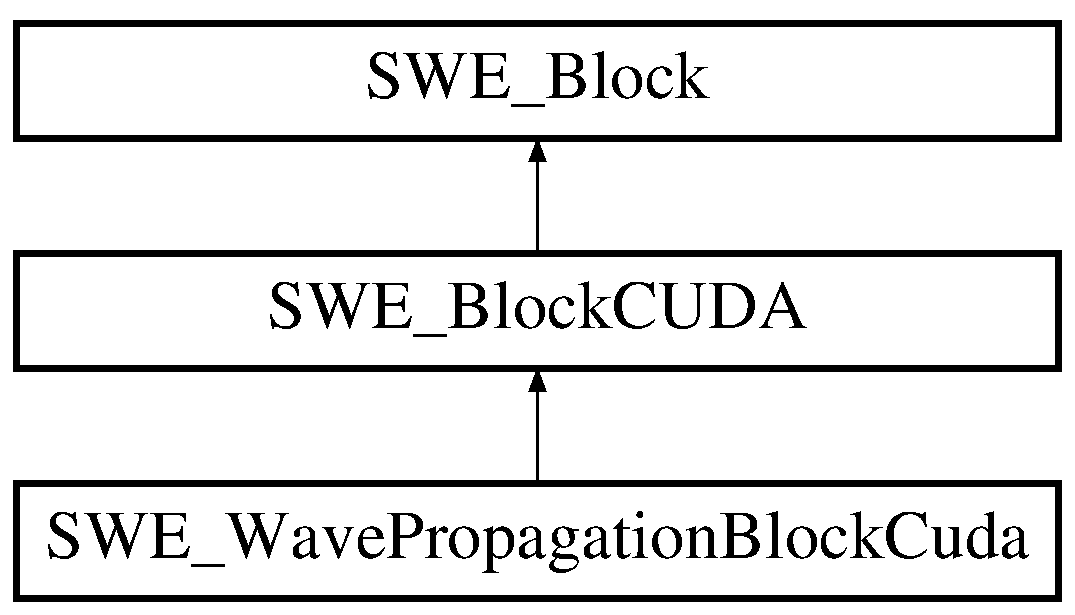
\includegraphics[height=3.000000cm]{classSWE__WavePropagationBlockCuda}
\end{center}
\end{figure}
\subsection*{Public Member Functions}
\begin{DoxyCompactItemize}
\item 
\hyperlink{classSWE__WavePropagationBlockCuda_a82f9de16ebab1bff58ead034416ab9ef}{S\-W\-E\-\_\-\-Wave\-Propagation\-Block\-Cuda} (int l\-\_\-nx, int l\-\_\-ny, float l\-\_\-dx, float l\-\_\-dy)
\item 
\hyperlink{classSWE__WavePropagationBlockCuda_ab4ad10c9704b7f5501f2a1d828672b57}{$\sim$\-S\-W\-E\-\_\-\-Wave\-Propagation\-Block\-Cuda} ()
\item 
void \hyperlink{classSWE__WavePropagationBlockCuda_ab401d17ea7a60ff30219076bc85dc591}{simulate\-Timestep} (float i\-\_\-d\-T)
\item 
float \hyperlink{classSWE__WavePropagationBlockCuda_a8c0fbb70ad29f3775d35978bf2d5b396}{simulate} (float, float)
\item 
void \hyperlink{classSWE__WavePropagationBlockCuda_a8a89bf61b9fc4433652f400ca8e564ed}{compute\-Numerical\-Fluxes} ()
\item 
void \hyperlink{classSWE__WavePropagationBlockCuda_a4163045a47a73515841e754ca3859fc5}{update\-Unknowns} (const float i\-\_\-delta\-T)
\end{DoxyCompactItemize}
\subsection*{Additional Inherited Members}


\subsection{Detailed Description}
\hyperlink{classSWE__WavePropagationBlockCuda}{S\-W\-E\-\_\-\-Wave\-Propagation\-Block\-Cuda} is an implementation of the S\-W\-E\-\_\-\-Block\-Cuda abstract class. It uses a wave propagation solver which is defined with the pre-\/compiler flag W\-A\-V\-E\-\_\-\-P\-R\-O\-P\-A\-G\-A\-T\-I\-O\-N\-\_\-\-S\-O\-L\-V\-E\-R (see above).

Possible wave propagation solvers are\-: F-\/\-Wave, $<$strike$>$Approximate Augmented Riemann, Hybrid (f-\/wave + augmented).$<$/strike$>$ (details can be found in the corresponding source files) 

\subsection{Constructor \& Destructor Documentation}
\hypertarget{classSWE__WavePropagationBlockCuda_a82f9de16ebab1bff58ead034416ab9ef}{\index{S\-W\-E\-\_\-\-Wave\-Propagation\-Block\-Cuda@{S\-W\-E\-\_\-\-Wave\-Propagation\-Block\-Cuda}!S\-W\-E\-\_\-\-Wave\-Propagation\-Block\-Cuda@{S\-W\-E\-\_\-\-Wave\-Propagation\-Block\-Cuda}}
\index{S\-W\-E\-\_\-\-Wave\-Propagation\-Block\-Cuda@{S\-W\-E\-\_\-\-Wave\-Propagation\-Block\-Cuda}!SWE_WavePropagationBlockCuda@{S\-W\-E\-\_\-\-Wave\-Propagation\-Block\-Cuda}}
\subsubsection[{S\-W\-E\-\_\-\-Wave\-Propagation\-Block\-Cuda}]{\setlength{\rightskip}{0pt plus 5cm}S\-W\-E\-\_\-\-Wave\-Propagation\-Block\-Cuda\-::\-S\-W\-E\-\_\-\-Wave\-Propagation\-Block\-Cuda (
\begin{DoxyParamCaption}
\item[{int}]{l\-\_\-nx, }
\item[{int}]{l\-\_\-ny, }
\item[{float}]{l\-\_\-dx, }
\item[{float}]{l\-\_\-dy}
\end{DoxyParamCaption}
)}}\label{classSWE__WavePropagationBlockCuda_a82f9de16ebab1bff58ead034416ab9ef}
Constructor of a \hyperlink{classSWE__WavePropagationBlockCuda}{S\-W\-E\-\_\-\-Wave\-Propagation\-Block\-Cuda}.

Allocates the variables for the simulation\-: Please note\-: The definition of indices changed in contrast to the C\-P\-U-\/\-Implementation.

unknowns hd,hud,hvd,bd stored on the C\-U\-D\-A device are defined for grid indices \mbox{[}0,..,nx+1\mbox{]}$\ast$\mbox{[}0,..,ny+1\mbox{]} (-\/$>$ Abstract class \hyperlink{classSWE__BlockCUDA}{S\-W\-E\-\_\-\-Block\-C\-U\-D\-A}) -\/$>$ computational domain is \mbox{[}1,..,nx\mbox{]}$\ast$\mbox{[}1,..,ny\mbox{]} -\/$>$ plus ghost cell layer

net-\/updates are defined for edges with indices \mbox{[}0,..,nx\mbox{]}$\ast$\mbox{[}0,..,ny\mbox{]} for horizontal and vertical edges for simplicity (one layer is not necessary).

A left/right net update with index (i-\/1,j) is located on the edge between cells with index (i-\/1,j) and (i,j)\-: 
\begin{DoxyPre}
  *********************
  *         *         *
  * (i-1,j) *  (i,j)  *
  *         *         *
  *********************\end{DoxyPre}



\begin{DoxyPre}            *
           ***
          *****
            *
            *
  NetUpdatesLeft(i-1,j)
            or
  NetUpdatesRight(i-1,j)
\end{DoxyPre}


A below/above net update with index (i, j-\/1) is located on the edge between cells with index (i, j-\/1) and (i,j)\-: 
\begin{DoxyPre}
  ***********
  *         *
  * (i, j)  *   *
  *         *  **  NetUpdatesBelow(i,j-1)
  *********** *****         or
  *         *  **  NetUpdatesAbove(i,j-1)
  * (i,j-1) *   *
  *         *
  ***********
\end{DoxyPre}
 
\begin{DoxyParams}{Parameters}
{\em i\-\_\-offset\-X} & spatial offset of the block in x-\/direction. \\
\hline
{\em i\-\_\-offset\-Y} & spatial offset of the offset in y-\/direction. \\
\hline
{\em i\-\_\-cuda\-Device} & I\-D of the C\-U\-D\-A-\/device, which should be used. \\
\hline
\end{DoxyParams}
\hypertarget{classSWE__WavePropagationBlockCuda_ab4ad10c9704b7f5501f2a1d828672b57}{\index{S\-W\-E\-\_\-\-Wave\-Propagation\-Block\-Cuda@{S\-W\-E\-\_\-\-Wave\-Propagation\-Block\-Cuda}!$\sim$\-S\-W\-E\-\_\-\-Wave\-Propagation\-Block\-Cuda@{$\sim$\-S\-W\-E\-\_\-\-Wave\-Propagation\-Block\-Cuda}}
\index{$\sim$\-S\-W\-E\-\_\-\-Wave\-Propagation\-Block\-Cuda@{$\sim$\-S\-W\-E\-\_\-\-Wave\-Propagation\-Block\-Cuda}!SWE_WavePropagationBlockCuda@{S\-W\-E\-\_\-\-Wave\-Propagation\-Block\-Cuda}}
\subsubsection[{$\sim$\-S\-W\-E\-\_\-\-Wave\-Propagation\-Block\-Cuda}]{\setlength{\rightskip}{0pt plus 5cm}S\-W\-E\-\_\-\-Wave\-Propagation\-Block\-Cuda\-::$\sim$\-S\-W\-E\-\_\-\-Wave\-Propagation\-Block\-Cuda (
\begin{DoxyParamCaption}
{}
\end{DoxyParamCaption}
)}}\label{classSWE__WavePropagationBlockCuda_ab4ad10c9704b7f5501f2a1d828672b57}
Destructor of a \hyperlink{classSWE__WavePropagationBlockCuda}{S\-W\-E\-\_\-\-Wave\-Propagation\-Block\-Cuda}.

Frees all of the memory, which was allocated within the constructor. Resets the C\-U\-D\-A device\-: Useful if error occured and printf is used on the device (buffer). 

\subsection{Member Function Documentation}
\hypertarget{classSWE__WavePropagationBlockCuda_a8a89bf61b9fc4433652f400ca8e564ed}{\index{S\-W\-E\-\_\-\-Wave\-Propagation\-Block\-Cuda@{S\-W\-E\-\_\-\-Wave\-Propagation\-Block\-Cuda}!compute\-Numerical\-Fluxes@{compute\-Numerical\-Fluxes}}
\index{compute\-Numerical\-Fluxes@{compute\-Numerical\-Fluxes}!SWE_WavePropagationBlockCuda@{S\-W\-E\-\_\-\-Wave\-Propagation\-Block\-Cuda}}
\subsubsection[{compute\-Numerical\-Fluxes}]{\setlength{\rightskip}{0pt plus 5cm}void S\-W\-E\-\_\-\-Wave\-Propagation\-Block\-Cuda\-::compute\-Numerical\-Fluxes (
\begin{DoxyParamCaption}
{}
\end{DoxyParamCaption}
)\hspace{0.3cm}{\ttfamily [virtual]}}}\label{classSWE__WavePropagationBlockCuda_a8a89bf61b9fc4433652f400ca8e564ed}
Compute the numerical fluxes (net-\/update formulation here) on all edges.

The maximum wave speed is computed within the net-\/updates kernel for each C\-U\-D\-A-\/block. To finalize the method the Thrust-\/library is called, which does the reduction over all blockwise maxima. In the wave speed reduction step the actual cell width in x-\/ and y-\/direction is not taken into account.

T\-O\-D\-O\-: A splitting or direct computation of the time step width might increase the total time step size. Example\-: dx = 11, dy = 6; max wave speed in x-\/direction\-: 10 max wave speed in y-\/direction\-: 5.\-5 max wave speed in both direction\-: 10

=$>$ maximum time step (current implementation)\-: min(11/10, 6/10) = 0.\-6 =$>$ maximum time step (splitting the dimensions)\-: min(11/10, 6/5.\-5) = 1.\-09.. {\bfseries Row-\/major vs column-\/major}

C/\-C++ arrays are row-\/major whereas warps are constructed in column-\/major order from threads/blocks. To get coalesced memory access in C\-U\-D\-A, we can use a 2-\/dimensional C\-U\-D\-A structure but we have to switch x and y inside a block.

This means, we have to switch thread\-Idx.\-x $<$-\/$>$ thread\-Idx.\-y as well as block\-Dim.\-x $<$-\/$>$ block\-Dim.\-y. Important\-: block\-Dim has to be switched for the kernel call as well!

definition of one C\-U\-D\-A-\/block. Typical size are 8$\ast$8 or 16$\ast$16

Definition of the \char`\"{}main\char`\"{} C\-U\-D\-A-\/grid. This grid covers only edges 0..\#(edges in x-\/direction)-\/2 and 0..\#(edges in y-\/direction)-\/2.

An example with a computational domain of size nx = 24, ny = 16 with a 1 cell ghost layer would result in a grid with (nx+2)$\ast$(ny+2) = (26$\ast$18) cells and (nx+1)$\ast$(ny+1) = (25$\ast$17) edges.

The C\-U\-D\-A-\/blocks (here 8$\ast$8) mentioned above would cover all edges except the ones lying between the computational domain and the right/top ghost layer\-: 
\begin{DoxyPre}
                                                         *
                                                        **        top ghost layer,
                                                       ********   cell ids
                       *******************************  **        = (*, ny+1)
                       *         *         *         *   *
                       *   8*8   *   8*8   *   8*8   *
                       *  block  *  block  *  block  *
                       *         *         *         *
                       *******************************
                       *         *         *         *
                       *   8*8   *   8*8   *   8*8   *
                   *   *  block  *  block  *  block  *
    bottom         **  *         *         *         *
    ghost     ******** *******************************
    layer,         **
    cell ids       *   *                              *
    =(*,0)            ***                            ***
                       *                              *
                       *                              *
                 left ghost layer,             right ghost layer,
                 cell ids = (0,*)             cell ids = (nx+1, *)
\end{DoxyPre}


Implements \hyperlink{classSWE__Block_a94dcf2c6ae31731e4586e45628b0c00e}{S\-W\-E\-\_\-\-Block}.

\hypertarget{classSWE__WavePropagationBlockCuda_a8c0fbb70ad29f3775d35978bf2d5b396}{\index{S\-W\-E\-\_\-\-Wave\-Propagation\-Block\-Cuda@{S\-W\-E\-\_\-\-Wave\-Propagation\-Block\-Cuda}!simulate@{simulate}}
\index{simulate@{simulate}!SWE_WavePropagationBlockCuda@{S\-W\-E\-\_\-\-Wave\-Propagation\-Block\-Cuda}}
\subsubsection[{simulate}]{\setlength{\rightskip}{0pt plus 5cm}\-\_\-\-\_\-host\-\_\-\-\_\- float S\-W\-E\-\_\-\-Wave\-Propagation\-Block\-Cuda\-::simulate (
\begin{DoxyParamCaption}
\item[{float}]{t\-Start, }
\item[{float}]{t\-End}
\end{DoxyParamCaption}
)\hspace{0.3cm}{\ttfamily [virtual]}}}\label{classSWE__WavePropagationBlockCuda_a8c0fbb70ad29f3775d35978bf2d5b396}
perform forward-\/\-Euler time steps, starting with simulation time t\-Start,\-: until simulation time t\-End is reached; device-\/global variables hd, hud, hvd are updated; unknowns h, hu, hv in main memory are not updated. Ghost layers and bathymetry sources are updated between timesteps. intended as main simulation loop between two checkpoints 

Reimplemented from \hyperlink{classSWE__Block_a69784e2be2d09035fb2af9d306768f07}{S\-W\-E\-\_\-\-Block}.

\hypertarget{classSWE__WavePropagationBlockCuda_ab401d17ea7a60ff30219076bc85dc591}{\index{S\-W\-E\-\_\-\-Wave\-Propagation\-Block\-Cuda@{S\-W\-E\-\_\-\-Wave\-Propagation\-Block\-Cuda}!simulate\-Timestep@{simulate\-Timestep}}
\index{simulate\-Timestep@{simulate\-Timestep}!SWE_WavePropagationBlockCuda@{S\-W\-E\-\_\-\-Wave\-Propagation\-Block\-Cuda}}
\subsubsection[{simulate\-Timestep}]{\setlength{\rightskip}{0pt plus 5cm}\-\_\-\-\_\-host\-\_\-\-\_\- void S\-W\-E\-\_\-\-Wave\-Propagation\-Block\-Cuda\-::simulate\-Timestep (
\begin{DoxyParamCaption}
\item[{float}]{i\-\_\-d\-T}
\end{DoxyParamCaption}
)\hspace{0.3cm}{\ttfamily [virtual]}}}\label{classSWE__WavePropagationBlockCuda_ab401d17ea7a60ff30219076bc85dc591}
Compute a single global time step of a given time step width. Remark\-: The user has to take care about the time step width. No additional check is done. The time step width typically available after the computation of the numerical fluxes (hidden in this method).

First the net-\/updates are computed. Then the cells are updated with the net-\/updates and the given time step width.


\begin{DoxyParams}{Parameters}
{\em i\-\_\-d\-T} & time step width in seconds. \\
\hline
\end{DoxyParams}


Reimplemented from \hyperlink{classSWE__Block_add6908e1ceb261a0a1f3ebc262cc5f11}{S\-W\-E\-\_\-\-Block}.

\hypertarget{classSWE__WavePropagationBlockCuda_a4163045a47a73515841e754ca3859fc5}{\index{S\-W\-E\-\_\-\-Wave\-Propagation\-Block\-Cuda@{S\-W\-E\-\_\-\-Wave\-Propagation\-Block\-Cuda}!update\-Unknowns@{update\-Unknowns}}
\index{update\-Unknowns@{update\-Unknowns}!SWE_WavePropagationBlockCuda@{S\-W\-E\-\_\-\-Wave\-Propagation\-Block\-Cuda}}
\subsubsection[{update\-Unknowns}]{\setlength{\rightskip}{0pt plus 5cm}void S\-W\-E\-\_\-\-Wave\-Propagation\-Block\-Cuda\-::update\-Unknowns (
\begin{DoxyParamCaption}
\item[{const float}]{i\-\_\-delta\-T}
\end{DoxyParamCaption}
)\hspace{0.3cm}{\ttfamily [virtual]}}}\label{classSWE__WavePropagationBlockCuda_a4163045a47a73515841e754ca3859fc5}
Update the cells with a given global time step.


\begin{DoxyParams}{Parameters}
{\em i\-\_\-delta\-T} & time step size. \\
\hline
\end{DoxyParams}
definition of one C\-U\-D\-A-\/block. Typical size are 8$\ast$8 or 16$\ast$16

definition of the C\-U\-D\-A-\/grid. 

Implements \hyperlink{classSWE__Block_ab2b4b659f23d5d45413dece8d2da3298}{S\-W\-E\-\_\-\-Block}.



The documentation for this class was generated from the following files\-:\begin{DoxyCompactItemize}
\item 
src/blocks/cuda/\hyperlink{SWE__WavePropagationBlockCuda_8hh}{S\-W\-E\-\_\-\-Wave\-Propagation\-Block\-Cuda.\-hh}\item 
src/blocks/cuda/\hyperlink{SWE__WavePropagationBlockCuda_8cu}{S\-W\-E\-\_\-\-Wave\-Propagation\-Block\-Cuda.\-cu}\end{DoxyCompactItemize}

\hypertarget{classSWE__WavePropagationBlockSIMD}{\section{S\-W\-E\-\_\-\-Wave\-Propagation\-Block\-S\-I\-M\-D Class Reference}
\label{classSWE__WavePropagationBlockSIMD}\index{S\-W\-E\-\_\-\-Wave\-Propagation\-Block\-S\-I\-M\-D@{S\-W\-E\-\_\-\-Wave\-Propagation\-Block\-S\-I\-M\-D}}
}


{\ttfamily \#include $<$S\-W\-E\-\_\-\-Wave\-Propagation\-Block\-S\-I\-M\-D.\-hh$>$}

Inheritance diagram for S\-W\-E\-\_\-\-Wave\-Propagation\-Block\-S\-I\-M\-D\-:\begin{figure}[H]
\begin{center}
\leavevmode
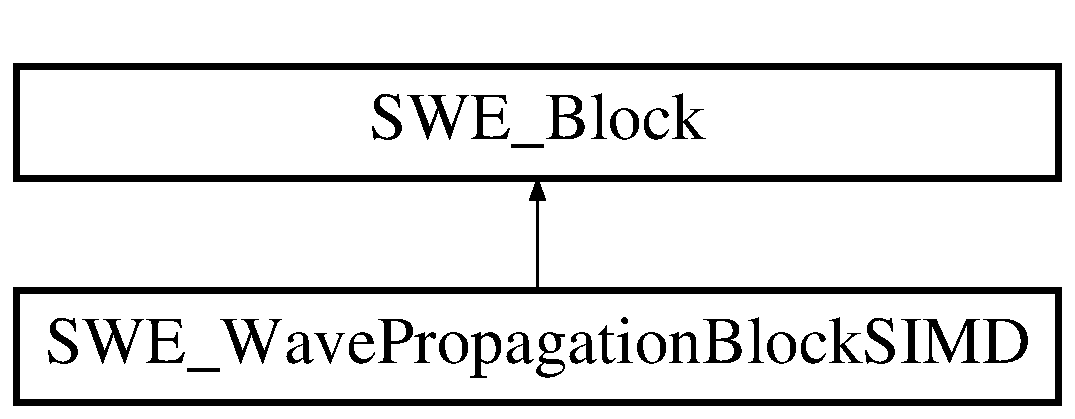
\includegraphics[height=2.000000cm]{classSWE__WavePropagationBlockSIMD}
\end{center}
\end{figure}
\subsection*{Public Member Functions}
\begin{DoxyCompactItemize}
\item 
\hyperlink{classSWE__WavePropagationBlockSIMD_a57dc616f1aa84f33a9c75ecb116b3228}{S\-W\-E\-\_\-\-Wave\-Propagation\-Block\-S\-I\-M\-D} (int l\-\_\-nx, int l\-\_\-ny, float l\-\_\-dx, float l\-\_\-dy)
\item 
virtual void \hyperlink{classSWE__WavePropagationBlockSIMD_a99c288632c402eaf7dff76f03624872a}{simulate\-Timestep} (float dt)
\item 
void \hyperlink{classSWE__WavePropagationBlockSIMD_a4aa15050ec1db113f54fff06539a900f}{compute\-Numerical\-Fluxes} ()
\item 
void \hyperlink{classSWE__WavePropagationBlockSIMD_a2596238868efd3cdd453d9ac2de15997}{update\-Unknowns} (float dt)
\item 
float \hyperlink{classSWE__WavePropagationBlockSIMD_a6c54dbcd43a77b46bae4de36b8d16af7}{simulate} (float i\-\_\-t\-Start, float i\-\_\-t\-End)
\item 
virtual \hyperlink{classSWE__WavePropagationBlockSIMD_aee73625ee731614849f398ea392137a7}{$\sim$\-S\-W\-E\-\_\-\-Wave\-Propagation\-Block\-S\-I\-M\-D} ()
\end{DoxyCompactItemize}
\subsection*{Additional Inherited Members}


\subsection{Detailed Description}
\hyperlink{classSWE__WavePropagationBlockSIMD}{S\-W\-E\-\_\-\-Wave\-Propagation\-Block\-S\-I\-M\-D} is an implementation of the \hyperlink{classSWE__Block}{S\-W\-E\-\_\-\-Block} abstract class. It uses a wave propagation solver which is defined with the pre-\/compiler flag W\-A\-V\-E\-\_\-\-P\-R\-O\-P\-A\-G\-A\-T\-I\-O\-N\-\_\-\-S\-O\-L\-V\-E\-R (see above).

Possible wave propagation solvers are\-: F-\/\-Wave, Apprximate Augmented Riemann, Hybrid (f-\/wave + augmented). (details can be found in the corresponding source files) 

\subsection{Constructor \& Destructor Documentation}
\hypertarget{classSWE__WavePropagationBlockSIMD_a57dc616f1aa84f33a9c75ecb116b3228}{\index{S\-W\-E\-\_\-\-Wave\-Propagation\-Block\-S\-I\-M\-D@{S\-W\-E\-\_\-\-Wave\-Propagation\-Block\-S\-I\-M\-D}!S\-W\-E\-\_\-\-Wave\-Propagation\-Block\-S\-I\-M\-D@{S\-W\-E\-\_\-\-Wave\-Propagation\-Block\-S\-I\-M\-D}}
\index{S\-W\-E\-\_\-\-Wave\-Propagation\-Block\-S\-I\-M\-D@{S\-W\-E\-\_\-\-Wave\-Propagation\-Block\-S\-I\-M\-D}!SWE_WavePropagationBlockSIMD@{S\-W\-E\-\_\-\-Wave\-Propagation\-Block\-S\-I\-M\-D}}
\subsubsection[{S\-W\-E\-\_\-\-Wave\-Propagation\-Block\-S\-I\-M\-D}]{\setlength{\rightskip}{0pt plus 5cm}S\-W\-E\-\_\-\-Wave\-Propagation\-Block\-S\-I\-M\-D\-::\-S\-W\-E\-\_\-\-Wave\-Propagation\-Block\-S\-I\-M\-D (
\begin{DoxyParamCaption}
\item[{int}]{l\-\_\-nx, }
\item[{int}]{l\-\_\-ny, }
\item[{float}]{l\-\_\-dx, }
\item[{float}]{l\-\_\-dy}
\end{DoxyParamCaption}
)}}\label{classSWE__WavePropagationBlockSIMD_a57dc616f1aa84f33a9c75ecb116b3228}
Constructor of a \hyperlink{classSWE__WavePropagationBlockSIMD}{S\-W\-E\-\_\-\-Wave\-Propagation\-Block\-S\-I\-M\-D}.

Allocates the variables for the simulation\-: unknowns h,hu,hv,b are defined on grid indices \mbox{[}0,..,nx+1\mbox{]}$\ast$\mbox{[}0,..,ny+1\mbox{]} (-\/$>$ Abstract class \hyperlink{classSWE__Block}{S\-W\-E\-\_\-\-Block}) -\/$>$ computational domain is \mbox{[}1,..,nx\mbox{]}$\ast$\mbox{[}1,..,ny\mbox{]} -\/$>$ plus ghost cell layer

net-\/updates are defined for edges with indices \mbox{[}0,..,nx\mbox{]}$\ast$\mbox{[}0,..,ny-\/1\mbox{]} or \mbox{[}0,..,nx-\/1\mbox{]}$\ast$\href{for horizontal/vertical edges}{\tt 0,..,ny}

A left/right net update with index (i-\/1,j-\/1) is located on the edge between cells with index (i-\/1,j) and (i,j)\-: 
\begin{DoxyPre}
  *********************
  *         *         *
  * (i-1,j) *  (i,j)  *
  *         *         *
  *********************\end{DoxyPre}



\begin{DoxyPre}            *
           ***
          *****
            *
            *
  NetUpdatesLeft(i-1,j-1)
            or
  NetUpdatesRight(i-1,j-1)
\end{DoxyPre}


A below/above net update with index (i-\/1, j-\/1) is located on the edge between cells with index (i, j-\/1) and (i,j)\-: 
\begin{DoxyPre}



  *         *
  * (i, j)  *   *
  *         *  **  NetUpdatesBelow(i-1,j-1)
  *********** *****         or
  *         *  **  NetUpdatesAbove(i-1,j-1)
  * (i,j-1) *   *
  *         *



\end{DoxyPre}
 \hypertarget{classSWE__WavePropagationBlockSIMD_aee73625ee731614849f398ea392137a7}{\index{S\-W\-E\-\_\-\-Wave\-Propagation\-Block\-S\-I\-M\-D@{S\-W\-E\-\_\-\-Wave\-Propagation\-Block\-S\-I\-M\-D}!$\sim$\-S\-W\-E\-\_\-\-Wave\-Propagation\-Block\-S\-I\-M\-D@{$\sim$\-S\-W\-E\-\_\-\-Wave\-Propagation\-Block\-S\-I\-M\-D}}
\index{$\sim$\-S\-W\-E\-\_\-\-Wave\-Propagation\-Block\-S\-I\-M\-D@{$\sim$\-S\-W\-E\-\_\-\-Wave\-Propagation\-Block\-S\-I\-M\-D}!SWE_WavePropagationBlockSIMD@{S\-W\-E\-\_\-\-Wave\-Propagation\-Block\-S\-I\-M\-D}}
\subsubsection[{$\sim$\-S\-W\-E\-\_\-\-Wave\-Propagation\-Block\-S\-I\-M\-D}]{\setlength{\rightskip}{0pt plus 5cm}virtual S\-W\-E\-\_\-\-Wave\-Propagation\-Block\-S\-I\-M\-D\-::$\sim$\-S\-W\-E\-\_\-\-Wave\-Propagation\-Block\-S\-I\-M\-D (
\begin{DoxyParamCaption}
{}
\end{DoxyParamCaption}
)\hspace{0.3cm}{\ttfamily [inline]}, {\ttfamily [virtual]}}}\label{classSWE__WavePropagationBlockSIMD_aee73625ee731614849f398ea392137a7}
Destructor of a \hyperlink{classSWE__WavePropagationBlockSIMD}{S\-W\-E\-\_\-\-Wave\-Propagation\-Block\-S\-I\-M\-D}.

In the case of a hybrid solver (N\-D\-E\-B\-U\-G not defined) information about the used solvers will be printed. 

\subsection{Member Function Documentation}
\hypertarget{classSWE__WavePropagationBlockSIMD_a4aa15050ec1db113f54fff06539a900f}{\index{S\-W\-E\-\_\-\-Wave\-Propagation\-Block\-S\-I\-M\-D@{S\-W\-E\-\_\-\-Wave\-Propagation\-Block\-S\-I\-M\-D}!compute\-Numerical\-Fluxes@{compute\-Numerical\-Fluxes}}
\index{compute\-Numerical\-Fluxes@{compute\-Numerical\-Fluxes}!SWE_WavePropagationBlockSIMD@{S\-W\-E\-\_\-\-Wave\-Propagation\-Block\-S\-I\-M\-D}}
\subsubsection[{compute\-Numerical\-Fluxes}]{\setlength{\rightskip}{0pt plus 5cm}void S\-W\-E\-\_\-\-Wave\-Propagation\-Block\-S\-I\-M\-D\-::compute\-Numerical\-Fluxes (
\begin{DoxyParamCaption}
{}
\end{DoxyParamCaption}
)\hspace{0.3cm}{\ttfamily [virtual]}}}\label{classSWE__WavePropagationBlockSIMD_a4aa15050ec1db113f54fff06539a900f}
Compute net updates for the block. The member variable \hyperlink{classSWE__Block_a05cbc9b40e0483bf73dbc2bdeae7dee3}{max\-Timestep} will be updated with the maximum allowed time step size 

Implements \hyperlink{classSWE__Block_a94dcf2c6ae31731e4586e45628b0c00e}{S\-W\-E\-\_\-\-Block}.

\hypertarget{classSWE__WavePropagationBlockSIMD_a6c54dbcd43a77b46bae4de36b8d16af7}{\index{S\-W\-E\-\_\-\-Wave\-Propagation\-Block\-S\-I\-M\-D@{S\-W\-E\-\_\-\-Wave\-Propagation\-Block\-S\-I\-M\-D}!simulate@{simulate}}
\index{simulate@{simulate}!SWE_WavePropagationBlockSIMD@{S\-W\-E\-\_\-\-Wave\-Propagation\-Block\-S\-I\-M\-D}}
\subsubsection[{simulate}]{\setlength{\rightskip}{0pt plus 5cm}float S\-W\-E\-\_\-\-Wave\-Propagation\-Block\-S\-I\-M\-D\-::simulate (
\begin{DoxyParamCaption}
\item[{float}]{i\-\_\-t\-Start, }
\item[{float}]{i\-\_\-t\-End}
\end{DoxyParamCaption}
)\hspace{0.3cm}{\ttfamily [virtual]}}}\label{classSWE__WavePropagationBlockSIMD_a6c54dbcd43a77b46bae4de36b8d16af7}
Runs the simulation until i\-\_\-t\-End is reached.


\begin{DoxyParams}{Parameters}
{\em i\-\_\-t\-Start} & time when the simulation starts \\
\hline
{\em i\-\_\-t\-End} & time when the simulation should end \\
\hline
\end{DoxyParams}
\begin{DoxyReturn}{Returns}
time we reached after the last update step, in general a bit later than i\-\_\-t\-End 
\end{DoxyReturn}


Reimplemented from \hyperlink{classSWE__Block_a69784e2be2d09035fb2af9d306768f07}{S\-W\-E\-\_\-\-Block}.

\hypertarget{classSWE__WavePropagationBlockSIMD_a99c288632c402eaf7dff76f03624872a}{\index{S\-W\-E\-\_\-\-Wave\-Propagation\-Block\-S\-I\-M\-D@{S\-W\-E\-\_\-\-Wave\-Propagation\-Block\-S\-I\-M\-D}!simulate\-Timestep@{simulate\-Timestep}}
\index{simulate\-Timestep@{simulate\-Timestep}!SWE_WavePropagationBlockSIMD@{S\-W\-E\-\_\-\-Wave\-Propagation\-Block\-S\-I\-M\-D}}
\subsubsection[{simulate\-Timestep}]{\setlength{\rightskip}{0pt plus 5cm}void S\-W\-E\-\_\-\-Wave\-Propagation\-Block\-S\-I\-M\-D\-::simulate\-Timestep (
\begin{DoxyParamCaption}
\item[{float}]{dt}
\end{DoxyParamCaption}
)\hspace{0.3cm}{\ttfamily [virtual]}}}\label{classSWE__WavePropagationBlockSIMD_a99c288632c402eaf7dff76f03624872a}
Update the bathymetry values with the displacement corresponding to the current time step.


\begin{DoxyParams}{Parameters}
{\em i\-\_\-asagi\-Scenario} & the corresponding A\-S\-A\-G\-I-\/scenario Executes a single timestep.
\begin{DoxyItemize}
\item compute net updates for every edge
\item update cell values with the net updates
\end{DoxyItemize}\\
\hline
{\em dt} & time step width of the update \\
\hline
\end{DoxyParams}


Reimplemented from \hyperlink{classSWE__Block_add6908e1ceb261a0a1f3ebc262cc5f11}{S\-W\-E\-\_\-\-Block}.

\hypertarget{classSWE__WavePropagationBlockSIMD_a2596238868efd3cdd453d9ac2de15997}{\index{S\-W\-E\-\_\-\-Wave\-Propagation\-Block\-S\-I\-M\-D@{S\-W\-E\-\_\-\-Wave\-Propagation\-Block\-S\-I\-M\-D}!update\-Unknowns@{update\-Unknowns}}
\index{update\-Unknowns@{update\-Unknowns}!SWE_WavePropagationBlockSIMD@{S\-W\-E\-\_\-\-Wave\-Propagation\-Block\-S\-I\-M\-D}}
\subsubsection[{update\-Unknowns}]{\setlength{\rightskip}{0pt plus 5cm}void S\-W\-E\-\_\-\-Wave\-Propagation\-Block\-S\-I\-M\-D\-::update\-Unknowns (
\begin{DoxyParamCaption}
\item[{float}]{dt}
\end{DoxyParamCaption}
)\hspace{0.3cm}{\ttfamily [virtual]}}}\label{classSWE__WavePropagationBlockSIMD_a2596238868efd3cdd453d9ac2de15997}
Updates the unknowns with the already computed net-\/updates.


\begin{DoxyParams}{Parameters}
{\em dt} & time step width used in the update. \\
\hline
\end{DoxyParams}


Implements \hyperlink{classSWE__Block_ab2b4b659f23d5d45413dece8d2da3298}{S\-W\-E\-\_\-\-Block}.



The documentation for this class was generated from the following files\-:\begin{DoxyCompactItemize}
\item 
src/blocks/\hyperlink{SWE__WavePropagationBlockSIMD_8hh}{S\-W\-E\-\_\-\-Wave\-Propagation\-Block\-S\-I\-M\-D.\-hh}\item 
src/blocks/\hyperlink{SWE__WavePropagationBlockSIMD_8cpp}{S\-W\-E\-\_\-\-Wave\-Propagation\-Block\-S\-I\-M\-D.\-cpp}\end{DoxyCompactItemize}

\hypertarget{classText}{\section{Text Class Reference}
\label{classText}\index{Text@{Text}}
}
\subsection*{Public Member Functions}
\begin{DoxyCompactItemize}
\item 
\hypertarget{classText_a26d2ab34aeb3b764b90221a473b4047f}{void {\bfseries add\-Text} (const char $\ast$text)}\label{classText_a26d2ab34aeb3b764b90221a473b4047f}

\item 
\hypertarget{classText_aff5cec718fcce7381d2d08717441af7f}{void {\bfseries start\-Text\-Mode} ()}\label{classText_aff5cec718fcce7381d2d08717441af7f}

\item 
bool \hyperlink{classText_a45299ae1fa870add85abe5f587428759}{show\-Next\-Text} (S\-D\-L\-\_\-\-Rect \&location)
\item 
\hypertarget{classText_a8f046f44006bf0a973b83cdc0d218e29}{void {\bfseries end\-Text\-Mode} ()}\label{classText_a8f046f44006bf0a973b83cdc0d218e29}

\end{DoxyCompactItemize}


\subsection{Member Function Documentation}
\hypertarget{classText_a45299ae1fa870add85abe5f587428759}{\index{Text@{Text}!show\-Next\-Text@{show\-Next\-Text}}
\index{show\-Next\-Text@{show\-Next\-Text}!Text@{Text}}
\subsubsection[{show\-Next\-Text}]{\setlength{\rightskip}{0pt plus 5cm}bool Text\-::show\-Next\-Text (
\begin{DoxyParamCaption}
\item[{S\-D\-L\-\_\-\-Rect \&}]{location}
\end{DoxyParamCaption}
)\hspace{0.3cm}{\ttfamily [inline]}}}\label{classText_a45299ae1fa870add85abe5f587428759}
\begin{DoxyReturn}{Returns}
True there are more textures 
\end{DoxyReturn}


The documentation for this class was generated from the following files\-:\begin{DoxyCompactItemize}
\item 
src/opengl/text.\-h\item 
src/opengl/text.\-cpp\end{DoxyCompactItemize}

\hypertarget{classtools_1_1Args}{\section{tools\-:\-:Args Class Reference}
\label{classtools_1_1Args}\index{tools\-::\-Args@{tools\-::\-Args}}
}


{\ttfamily \#include $<$args.\-hh$>$}

\subsection*{Public Types}
\begin{DoxyCompactItemize}
\item 
enum {\bfseries Argument} \{ {\bfseries Required} = required\-\_\-argument, 
{\bfseries No} = no\-\_\-argument, 
{\bfseries Optional} = optional\-\_\-argument
 \}
\item 
enum \hyperlink{classtools_1_1Args_ae0b38617134893616df504e543ba6e6e}{Result} \{ {\bfseries Success} = 0, 
{\bfseries Error}, 
\hyperlink{classtools_1_1Args_ae0b38617134893616df504e543ba6e6ea3be887fb99c1931485e91a4e0bdcf539}{Help}
 \}
\end{DoxyCompactItemize}
\subsection*{Public Member Functions}
\begin{DoxyCompactItemize}
\item 
\hypertarget{classtools_1_1Args_ac990064dc296955154be98d98acd46b9}{{\bfseries Args} (const std\-::string \&description=\char`\"{}\char`\"{}, bool add\-Help=true)}\label{classtools_1_1Args_ac990064dc296955154be98d98acd46b9}

\item 
\hypertarget{classtools_1_1Args_a10d5693fa13e60f9da62dcd8696c150d}{void {\bfseries add\-Option} (const std\-::string \&long\-Option, char short\-Option=0, const std\-::string \&description=\char`\"{}\char`\"{}, Argument argument=Required, bool required=true)}\label{classtools_1_1Args_a10d5693fa13e60f9da62dcd8696c150d}

\item 
\hyperlink{classtools_1_1Args_ae0b38617134893616df504e543ba6e6e}{Result} \hyperlink{classtools_1_1Args_a9d8751d3ca13ddf37d390f42384ba49a}{parse} (int argc, char $\ast$const $\ast$argv, bool print\-Help=true)
\item 
\hypertarget{classtools_1_1Args_a73558f89ba2c7592c0bbb5c29bee228c}{bool {\bfseries is\-Set} (const std\-::string \&option)}\label{classtools_1_1Args_a73558f89ba2c7592c0bbb5c29bee228c}

\item 
\hypertarget{classtools_1_1Args_ab21287411ac81cd228184ee520267851}{{\footnotesize template$<$typename T $>$ }\\T {\bfseries get\-Argument} (const std\-::string \&option)}\label{classtools_1_1Args_ab21287411ac81cd228184ee520267851}

\item 
\hypertarget{classtools_1_1Args_a6247cd94f3bc79ce2a120777caeaea7c}{{\footnotesize template$<$typename T $>$ }\\T {\bfseries get\-Argument} (const std\-::string \&option, T default\-Argument)}\label{classtools_1_1Args_a6247cd94f3bc79ce2a120777caeaea7c}

\item 
\hypertarget{classtools_1_1Args_a8e805f57e66ed5407fe3762b8409d685}{void {\bfseries help\-Message} (const char $\ast$prog, std\-::ostream \&out=std\-::cout)}\label{classtools_1_1Args_a8e805f57e66ed5407fe3762b8409d685}

\item 
\hypertarget{classtools_1_1Args_ab9c570cfa217f4694ac801de1e835351}{{\footnotesize template$<$$>$ }\\std\-::string {\bfseries get\-Argument} (const std\-::string \&option)}\label{classtools_1_1Args_ab9c570cfa217f4694ac801de1e835351}

\end{DoxyCompactItemize}


\subsection{Detailed Description}
Parses command line arguments 

\subsection{Member Enumeration Documentation}
\hypertarget{classtools_1_1Args_ae0b38617134893616df504e543ba6e6e}{\index{tools\-::\-Args@{tools\-::\-Args}!Result@{Result}}
\index{Result@{Result}!tools::Args@{tools\-::\-Args}}
\subsubsection[{Result}]{\setlength{\rightskip}{0pt plus 5cm}enum {\bf tools\-::\-Args\-::\-Result}}}\label{classtools_1_1Args_ae0b38617134893616df504e543ba6e6e}
\begin{Desc}
\item[Enumerator]\par
\begin{description}
\index{Help@{Help}!tools\-::\-Args@{tools\-::\-Args}}\index{tools\-::\-Args@{tools\-::\-Args}!Help@{Help}}\item[{\em 
\hypertarget{classtools_1_1Args_ae0b38617134893616df504e543ba6e6ea3be887fb99c1931485e91a4e0bdcf539}{Help}\label{classtools_1_1Args_ae0b38617134893616df504e543ba6e6ea3be887fb99c1931485e91a4e0bdcf539}
}]Help message printed \end{description}
\end{Desc}


\subsection{Member Function Documentation}
\hypertarget{classtools_1_1Args_a9d8751d3ca13ddf37d390f42384ba49a}{\index{tools\-::\-Args@{tools\-::\-Args}!parse@{parse}}
\index{parse@{parse}!tools::Args@{tools\-::\-Args}}
\subsubsection[{parse}]{\setlength{\rightskip}{0pt plus 5cm}{\bf Result} tools\-::\-Args\-::parse (
\begin{DoxyParamCaption}
\item[{int}]{argc, }
\item[{char $\ast$const $\ast$}]{argv, }
\item[{bool}]{print\-Help = {\ttfamily true}}
\end{DoxyParamCaption}
)\hspace{0.3cm}{\ttfamily [inline]}}}\label{classtools_1_1Args_a9d8751d3ca13ddf37d390f42384ba49a}
\begin{DoxyReturn}{Returns}
True of options are successfully parsed, false otherwise 
\end{DoxyReturn}


The documentation for this class was generated from the following file\-:\begin{DoxyCompactItemize}
\item 
src/tools/\hyperlink{args_8hh}{args.\-hh}\end{DoxyCompactItemize}

\hypertarget{classtools_1_1Logger}{\section{tools\-:\-:Logger Class Reference}
\label{classtools_1_1Logger}\index{tools\-::\-Logger@{tools\-::\-Logger}}
}
\subsection*{Public Member Functions}
\begin{DoxyCompactItemize}
\item 
\hyperlink{classtools_1_1Logger_a9e1e0651776fcc78f89a1a1dcf339249}{Logger} (const int i\-\_\-process\-Rank=0, const std\-::string i\-\_\-program\-Name=\char`\"{}S\-W\-E\char`\"{}, const std\-::string i\-\_\-welcome\-Message=\char`\"{}Welcome to\char`\"{}, const std\-::string i\-\_\-copy\-Rights=\char`\"{}\textbackslash{}n\textbackslash{}n\-S\-W\-E Copyright (C) 2012-\/2013\textbackslash{}n\char`\"{}\char`\"{}  Technische Universitaet Muenchen\textbackslash{}n\char`\"{}\char`\"{}  Department of Informatics\textbackslash{}n\char`\"{}\char`\"{}  Chair of Scientific Computing\textbackslash{}n\char`\"{}\char`\"{}  http\-://www5.\-in.\-tum.\-de/S\-W\-E\textbackslash{}n\char`\"{}\char`\"{}\textbackslash{}n\char`\"{}\char`\"{}S\-W\-E comes with A\-B\-S\-O\-L\-U\-T\-E\-L\-Y N\-O W\-A\-R\-R\-A\-N\-T\-Y.\textbackslash{}n\char`\"{}\char`\"{}S\-W\-E is free software, and you are welcome to redistribute it\textbackslash{}n\char`\"{}\char`\"{}under certain conditions.\textbackslash{}n\char`\"{}\char`\"{}Details can be found in the file \textbackslash{}'gpl.\-txt\textbackslash{}'.\char`\"{}, const std\-::string i\-\_\-finish\-Message=\char`\"{}finished successfully.\char`\"{}, const std\-::string i\-\_\-mid\-Delimiter=\char`\"{}\textbackslash{}n-\/-\/-\/-\/-\/-\/-\/-\/-\/-\/-\/-\/-\/-\/-\/-\/-\/-\/-\/-\/-\/-\/-\/-\/-\/-\/-\/-\/-\/-\/-\/-\/-\/-\/-\/-\/-\/-\/-\/-\/-\/-\/-\/-\/-\/-\/-\/-\/-\/-\/-\/-\/-\/-\/-\/-\/-\/-\/-\/-\/-\/-\/-\/-\/-\/-\/\textbackslash{}n\char`\"{}, const std\-::string i\-\_\-large\-Delimiter=\char`\"{}\textbackslash{}n$\ast$$\ast$$\ast$$\ast$$\ast$$\ast$$\ast$$\ast$$\ast$$\ast$$\ast$$\ast$$\ast$$\ast$$\ast$$\ast$$\ast$$\ast$$\ast$$\ast$$\ast$$\ast$$\ast$$\ast$$\ast$$\ast$$\ast$$\ast$$\ast$$\ast$$\ast$$\ast$$\ast$$\ast$$\ast$$\ast$$\ast$$\ast$$\ast$$\ast$$\ast$$\ast$$\ast$$\ast$$\ast$$\ast$$\ast$$\ast$$\ast$$\ast$$\ast$$\ast$$\ast$$\ast$$\ast$$\ast$$\ast$$\ast$$\ast$$\ast$$\ast$\textbackslash{}n\char`\"{}, const std\-::string i\-\_\-indentation=\char`\"{}\textbackslash{}t\char`\"{})
\item 
virtual \hyperlink{classtools_1_1Logger_a58f170bf361ba7ceb3a4e0d9ec36bdf5}{$\sim$\-Logger} ()
\item 
void \hyperlink{classtools_1_1Logger_af45e7a1b4e9c33ab9fbb43e18e284eae}{print\-Welcome\-Message} ()
\item 
void \hyperlink{classtools_1_1Logger_a539d6f7c8e60c0ee887912c92c1dfa5c}{print\-Finish\-Message} ()
\item 
std\-::ostream \& \hyperlink{classtools_1_1Logger_ab0d82d23125a3d5d8b737984e678f43a}{cout} ()
\item 
void \hyperlink{classtools_1_1Logger_a1d3e0fcc3cb4c58eb486ac3fe14d30b0}{set\-Process\-Rank} (const int i\-\_\-process\-Rank)
\item 
void \hyperlink{classtools_1_1Logger_a9642689522ece27ca9c908f24f290134}{print\-String} (const std\-::string i\-\_\-string)
\item 
void \hyperlink{classtools_1_1Logger_a89b9dfd5340a4e18d7b8f1225d996730}{print\-Number\-Of\-Processes} (const int i\-\_\-number\-Of\-Processes, const std\-::string i\-\_\-processes\-Name=\char`\"{}M\-P\-I processes\char`\"{})
\item 
void \hyperlink{classtools_1_1Logger_a2da0a6c575304e91bea546dddc94f72d}{print\-Number\-Of\-Cells} (const int i\-\_\-n\-X, const int i\-\_\-n\-Y, const std\-::string i\-\_\-cell\-Message=\char`\"{}cells\char`\"{})
\item 
void \hyperlink{classtools_1_1Logger_acf2b4547c8b138e4e8e338002687a149}{print\-Number\-Of\-Cells\-Per\-Process} (const int i\-\_\-n\-X, const int i\-\_\-n\-Y)
\item 
void \hyperlink{classtools_1_1Logger_a4c81063c055f072c465853d6da85743b}{print\-Cell\-Size} (const float i\-\_\-d\-X, const float i\-\_\-d\-Y, const std\-::string i\-\_\-unit=\char`\"{}m\char`\"{})
\item 
void \hyperlink{classtools_1_1Logger_a6c71eab182524a84037eb6fe1ac42e9e}{print\-Number\-Of\-Blocks} (const int i\-\_\-n\-X, const int i\-\_\-n\-Y)
\item 
void \hyperlink{classtools_1_1Logger_a2d54396c65885248374009cb3b18c2da}{print\-Start\-Message} (const std\-::string i\-\_\-start\-Message=\char`\"{}Everything is set up, starting the simulation.\char`\"{})
\item 
void \hyperlink{classtools_1_1Logger_ac829729cc06f2a6e43f0272ada747685}{print\-Simulation\-Time} (const float i\-\_\-time, const std\-::string i\-\_\-simulation\-Time\-Message=\char`\"{}Simulation at time\char`\"{})
\item 
void \hyperlink{classtools_1_1Logger_aec0d76a09748963c9f0b68239e4499c0}{print\-Output\-File\-Creation} (const std\-::string i\-\_\-file\-Name, const int i\-\_\-block\-X, const int i\-\_\-block\-Y, const std\-::string i\-\_\-file\-Type=\char`\"{}net\-C\-D\-F\char`\"{})
\item 
void \hyperlink{classtools_1_1Logger_ab7f380c82631174ff826dfd8bf519058}{print\-Output\-Time} (const float i\-\_\-time, const std\-::string i\-\_\-output\-Time\-Message=\char`\"{}Writing output file at time\char`\"{})
\item 
void \hyperlink{classtools_1_1Logger_a6030321e16a66849dbf237420702a0da}{print\-Statistics\-Message} (const std\-::string i\-\_\-statistics\-Message=\char`\"{}Simulation finished. Printing statistics for each process.\char`\"{})
\item 
void \hyperlink{classtools_1_1Logger_a6f23f0f674d0e7bbf1a52442eff5c031}{print\-Solver\-Statistics} (const long i\-\_\-first\-Solver\-Counter, const long i\-\_\-second\-Solver\-Counter, const int i\-\_\-block\-X=0, const int i\-\_\-block\-Y=0, const std\-::string i\-\_\-first\-Solver\-Name=\char`\"{}f-\/Wave solver\char`\"{}, const std\-::string i\-\_\-second\-Solver\-Name=\char`\"{}Augemented Riemann solver\char`\"{})
\item 
void \hyperlink{classtools_1_1Logger_ad5986d50f6c7bec49b9d07e9b1e7ac1b}{update\-Time} (const std\-::string \&i\-\_\-name)
\item 
void \hyperlink{classtools_1_1Logger_a46e0d98ad67c8ac1d26ff8d695c5fceb}{reset\-Clock\-To\-Current\-Time} (const std\-::string \&i\-\_\-name)
\item 
void \hyperlink{classtools_1_1Logger_ab1bb09a74580560b36c19979d88ef3bc}{init\-Wall\-Clock\-Time} (const double i\-\_\-wall\-Clock\-Time)
\item 
void \hyperlink{classtools_1_1Logger_a432c4dbdbc532bc792cd0d4b30b3b42e}{print\-Wall\-Clock\-Time} (const double i\-\_\-wall\-Clock\-Time, const std\-::string i\-\_\-wall\-Clock\-Time\-Message=\char`\"{}wall clock time\char`\"{})
\item 
void \hyperlink{classtools_1_1Logger_a538f0d1e94f6a957a8936d663f56859c}{print\-Time} (const std\-::string \&i\-\_\-name, const std\-::string \&i\-\_\-message)
\item 
double \hyperlink{classtools_1_1Logger_a01a480f7c6ce911114529b193188f211}{get\-Time} (const std\-::string \&i\-\_\-name)
\item 
void \hyperlink{classtools_1_1Logger_a2e9f836ab40bfde976770aa711b8547d}{print\-Iterations\-Done} (unsigned int i\-\_\-iterations, std\-::string i\-\_\-iteration\-Message=\char`\"{}iterations done\char`\"{})
\item 
void \hyperlink{classtools_1_1Logger_aff8aabe69fd994258cf5238ff0e1f55f}{print\-Element\-Updates\-Done} (unsigned int i\-\_\-iterations, const int i\-\_\-n\-X, const int i\-\_\-n\-Y, const std\-::string \&i\-\_\-name, const std\-::string i\-\_\-iteration\-Message=\char`\"{}element updates per second done\char`\"{})
\end{DoxyCompactItemize}
\subsection*{Static Public Attributes}
\begin{DoxyCompactItemize}
\item 
static \hyperlink{classtools_1_1Logger}{Logger} \hyperlink{classtools_1_1Logger_a341eaab3865b60362db6736c2e2b7c68}{logger}
\end{DoxyCompactItemize}


\subsection{Constructor \& Destructor Documentation}
\hypertarget{classtools_1_1Logger_a9e1e0651776fcc78f89a1a1dcf339249}{\index{tools\-::\-Logger@{tools\-::\-Logger}!Logger@{Logger}}
\index{Logger@{Logger}!tools::Logger@{tools\-::\-Logger}}
\subsubsection[{Logger}]{\setlength{\rightskip}{0pt plus 5cm}tools\-::\-Logger\-::\-Logger (
\begin{DoxyParamCaption}
\item[{const int}]{i\-\_\-process\-Rank = {\ttfamily 0}, }
\item[{const std\-::string}]{i\-\_\-program\-Name = {\ttfamily \char`\"{}SWE\char`\"{}}, }
\item[{const std\-::string}]{i\-\_\-welcome\-Message = {\ttfamily \char`\"{}Welcome~to\char`\"{}}, }
\item[{const std\-::string}]{i\-\_\-copy\-Rights = {\ttfamily \char`\"{}\textbackslash{}n\textbackslash{}nSWE~Copyright~(C)~2012-\/2013\textbackslash{}n\char`\"{}~\char`\"{}~~Technische~Universitaet~Muenchen\textbackslash{}n\char`\"{}~\char`\"{}~~Department~of~Informatics\textbackslash{}n\char`\"{}~\char`\"{}~~Chair~of~Scientific~Computing\textbackslash{}n\char`\"{}~\char`\"{}~~http\-://www5.in.tum.de/SWE\textbackslash{}n\char`\"{}~\char`\"{}\textbackslash{}n\char`\"{}~\char`\"{}SWE~comes~with~ABSOLUTELY~NO~WARRANTY.\textbackslash{}n\char`\"{}~\char`\"{}SWE~is~free~software,~and~you~are~welcome~to~redistribute~it\textbackslash{}n\char`\"{}~\char`\"{}under~certain~conditions.\textbackslash{}n\char`\"{}~\char`\"{}Details~can~be~found~in~the~file~\textbackslash{}'gpl.txt\textbackslash{}'.\char`\"{}}, }
\item[{const std\-::string}]{i\-\_\-finish\-Message = {\ttfamily \char`\"{}finished~successfully.\char`\"{}}, }
\item[{const std\-::string}]{i\-\_\-mid\-Delimiter = {\ttfamily \char`\"{}\textbackslash{}n-\/-\/-\/-\/-\/-\/-\/-\/-\/-\/-\/-\/-\/-\/-\/-\/-\/-\/-\/-\/-\/-\/-\/-\/-\/-\/-\/-\/-\/-\/-\/-\/-\/-\/-\/-\/-\/-\/-\/-\/-\/-\/-\/-\/-\/-\/-\/-\/-\/-\/-\/-\/-\/-\/-\/-\/-\/-\/-\/-\/-\/-\/-\/-\/-\/-\/\textbackslash{}n\char`\"{}}, }
\item[{const std\-::string}]{i\-\_\-large\-Delimiter = {\ttfamily \char`\"{}\textbackslash{}n$\ast$$\ast$$\ast$$\ast$$\ast$$\ast$$\ast$$\ast$$\ast$$\ast$$\ast$$\ast$$\ast$$\ast$$\ast$$\ast$$\ast$$\ast$$\ast$$\ast$$\ast$$\ast$$\ast$$\ast$$\ast$$\ast$$\ast$$\ast$$\ast$$\ast$$\ast$$\ast$$\ast$$\ast$$\ast$$\ast$$\ast$$\ast$$\ast$$\ast$$\ast$$\ast$$\ast$$\ast$$\ast$$\ast$$\ast$$\ast$$\ast$$\ast$$\ast$$\ast$$\ast$$\ast$$\ast$$\ast$$\ast$$\ast$$\ast$$\ast$$\ast$\textbackslash{}n\char`\"{}}, }
\item[{const std\-::string}]{i\-\_\-indentation = {\ttfamily \char`\"{}\textbackslash{}t\char`\"{}}}
\end{DoxyParamCaption}
)\hspace{0.3cm}{\ttfamily [inline]}}}\label{classtools_1_1Logger_a9e1e0651776fcc78f89a1a1dcf339249}
The Constructor. Prints the welcome message (process rank 0 only).


\begin{DoxyParams}{Parameters}
{\em i\-\_\-process\-Rank} & rank of the constructing process. \\
\hline
{\em i\-\_\-program\-Name} & definition of the program name. \\
\hline
{\em i\-\_\-welcome\-Message} & definition of the welcome message. \\
\hline
{\em i\-\_\-start\-Message} & definition of the start message. \\
\hline
{\em i\-\_\-simulation\-Time\-Message} & definition of the simulation time message. \\
\hline
{\em i\-\_\-execution\-Time\-Message} & definition of the execution time message. \\
\hline
{\em i\-\_\-cpu\-Time\-Message} & definition of the C\-P\-U time message. \\
\hline
{\em i\-\_\-finish\-Message} & definition of the finish message. \\
\hline
{\em i\-\_\-mid\-Delimiter} & definition of the mid-\/size delimiter. \\
\hline
{\em i\-\_\-large\-Delimiter} & definition of the large delimiter. \\
\hline
{\em i\-\_\-indentation} & definition of the indentation (used in all messages, except welcome, start and finish). \\
\hline
\end{DoxyParams}
\hypertarget{classtools_1_1Logger_a58f170bf361ba7ceb3a4e0d9ec36bdf5}{\index{tools\-::\-Logger@{tools\-::\-Logger}!$\sim$\-Logger@{$\sim$\-Logger}}
\index{$\sim$\-Logger@{$\sim$\-Logger}!tools::Logger@{tools\-::\-Logger}}
\subsubsection[{$\sim$\-Logger}]{\setlength{\rightskip}{0pt plus 5cm}virtual tools\-::\-Logger\-::$\sim$\-Logger (
\begin{DoxyParamCaption}
{}
\end{DoxyParamCaption}
)\hspace{0.3cm}{\ttfamily [inline]}, {\ttfamily [virtual]}}}\label{classtools_1_1Logger_a58f170bf361ba7ceb3a4e0d9ec36bdf5}
The Destructor. Prints the finish message (process rank 0 only). 

\subsection{Member Function Documentation}
\hypertarget{classtools_1_1Logger_ab0d82d23125a3d5d8b737984e678f43a}{\index{tools\-::\-Logger@{tools\-::\-Logger}!cout@{cout}}
\index{cout@{cout}!tools::Logger@{tools\-::\-Logger}}
\subsubsection[{cout}]{\setlength{\rightskip}{0pt plus 5cm}std\-::ostream\& tools\-::\-Logger\-::cout (
\begin{DoxyParamCaption}
{}
\end{DoxyParamCaption}
)\hspace{0.3cm}{\ttfamily [inline]}}}\label{classtools_1_1Logger_ab0d82d23125a3d5d8b737984e678f43a}
Default output stream of the logger.

\begin{DoxyReturn}{Returns}
extended (time + indentation) std\-::cout stream. 
\end{DoxyReturn}
\hypertarget{classtools_1_1Logger_a01a480f7c6ce911114529b193188f211}{\index{tools\-::\-Logger@{tools\-::\-Logger}!get\-Time@{get\-Time}}
\index{get\-Time@{get\-Time}!tools::Logger@{tools\-::\-Logger}}
\subsubsection[{get\-Time}]{\setlength{\rightskip}{0pt plus 5cm}double tools\-::\-Logger\-::get\-Time (
\begin{DoxyParamCaption}
\item[{const std\-::string \&}]{i\-\_\-name}
\end{DoxyParamCaption}
)\hspace{0.3cm}{\ttfamily [inline]}}}\label{classtools_1_1Logger_a01a480f7c6ce911114529b193188f211}
Get elapsed time


\begin{DoxyParams}{Parameters}
{\em i\-\_\-name} & Name of the time \\
\hline
\end{DoxyParams}
\begin{DoxyReturn}{Returns}
elapsed time 
\end{DoxyReturn}
\hypertarget{classtools_1_1Logger_ab1bb09a74580560b36c19979d88ef3bc}{\index{tools\-::\-Logger@{tools\-::\-Logger}!init\-Wall\-Clock\-Time@{init\-Wall\-Clock\-Time}}
\index{init\-Wall\-Clock\-Time@{init\-Wall\-Clock\-Time}!tools::Logger@{tools\-::\-Logger}}
\subsubsection[{init\-Wall\-Clock\-Time}]{\setlength{\rightskip}{0pt plus 5cm}void tools\-::\-Logger\-::init\-Wall\-Clock\-Time (
\begin{DoxyParamCaption}
\item[{const double}]{i\-\_\-wall\-Clock\-Time}
\end{DoxyParamCaption}
)\hspace{0.3cm}{\ttfamily [inline]}}}\label{classtools_1_1Logger_ab1bb09a74580560b36c19979d88ef3bc}
Initialize the wall clock time.


\begin{DoxyParams}{Parameters}
{\em i\-\_\-wall\-Clock\-Time} & value the wall block time will be set to. \\
\hline
\end{DoxyParams}
\hypertarget{classtools_1_1Logger_a4c81063c055f072c465853d6da85743b}{\index{tools\-::\-Logger@{tools\-::\-Logger}!print\-Cell\-Size@{print\-Cell\-Size}}
\index{print\-Cell\-Size@{print\-Cell\-Size}!tools::Logger@{tools\-::\-Logger}}
\subsubsection[{print\-Cell\-Size}]{\setlength{\rightskip}{0pt plus 5cm}void tools\-::\-Logger\-::print\-Cell\-Size (
\begin{DoxyParamCaption}
\item[{const float}]{i\-\_\-d\-X, }
\item[{const float}]{i\-\_\-d\-Y, }
\item[{const std\-::string}]{i\-\_\-unit = {\ttfamily \char`\"{}m\char`\"{}}}
\end{DoxyParamCaption}
)\hspace{0.3cm}{\ttfamily [inline]}}}\label{classtools_1_1Logger_a4c81063c055f072c465853d6da85743b}
Print the size of a cell


\begin{DoxyParams}{Parameters}
{\em i\-\_\-d\-X} & size in x-\/direction. \\
\hline
{\em i\-\_\-d\-Y} & size in y-\/direction. \\
\hline
{\em i\-\_\-unit} & measurement unit. \\
\hline
\end{DoxyParams}
\hypertarget{classtools_1_1Logger_aff8aabe69fd994258cf5238ff0e1f55f}{\index{tools\-::\-Logger@{tools\-::\-Logger}!print\-Element\-Updates\-Done@{print\-Element\-Updates\-Done}}
\index{print\-Element\-Updates\-Done@{print\-Element\-Updates\-Done}!tools::Logger@{tools\-::\-Logger}}
\subsubsection[{print\-Element\-Updates\-Done}]{\setlength{\rightskip}{0pt plus 5cm}void tools\-::\-Logger\-::print\-Element\-Updates\-Done (
\begin{DoxyParamCaption}
\item[{unsigned int}]{i\-\_\-iterations, }
\item[{const int}]{i\-\_\-n\-X, }
\item[{const int}]{i\-\_\-n\-Y, }
\item[{const std\-::string \&}]{i\-\_\-name, }
\item[{const std\-::string}]{i\-\_\-iteration\-Message = {\ttfamily \char`\"{}element~updates~per~second~done\char`\"{}}}
\end{DoxyParamCaption}
)\hspace{0.3cm}{\ttfamily [inline]}}}\label{classtools_1_1Logger_aff8aabe69fd994258cf5238ff0e1f55f}
Print number of element updates done


\begin{DoxyParams}{Parameters}
{\em i\-\_\-iterations} & Number of iterations done \\
\hline
{\em i\-\_\-interation\-Message} & Iterations done message \\
\hline
\end{DoxyParams}
\hypertarget{classtools_1_1Logger_a539d6f7c8e60c0ee887912c92c1dfa5c}{\index{tools\-::\-Logger@{tools\-::\-Logger}!print\-Finish\-Message@{print\-Finish\-Message}}
\index{print\-Finish\-Message@{print\-Finish\-Message}!tools::Logger@{tools\-::\-Logger}}
\subsubsection[{print\-Finish\-Message}]{\setlength{\rightskip}{0pt plus 5cm}void tools\-::\-Logger\-::print\-Finish\-Message (
\begin{DoxyParamCaption}
{}
\end{DoxyParamCaption}
)\hspace{0.3cm}{\ttfamily [inline]}}}\label{classtools_1_1Logger_a539d6f7c8e60c0ee887912c92c1dfa5c}
Print the finish message. \hypertarget{classtools_1_1Logger_a2e9f836ab40bfde976770aa711b8547d}{\index{tools\-::\-Logger@{tools\-::\-Logger}!print\-Iterations\-Done@{print\-Iterations\-Done}}
\index{print\-Iterations\-Done@{print\-Iterations\-Done}!tools::Logger@{tools\-::\-Logger}}
\subsubsection[{print\-Iterations\-Done}]{\setlength{\rightskip}{0pt plus 5cm}void tools\-::\-Logger\-::print\-Iterations\-Done (
\begin{DoxyParamCaption}
\item[{unsigned int}]{i\-\_\-iterations, }
\item[{std\-::string}]{i\-\_\-iteration\-Message = {\ttfamily \char`\"{}iterations~done\char`\"{}}}
\end{DoxyParamCaption}
)\hspace{0.3cm}{\ttfamily [inline]}}}\label{classtools_1_1Logger_a2e9f836ab40bfde976770aa711b8547d}
Print number of iterations done


\begin{DoxyParams}{Parameters}
{\em i\-\_\-iterations} & Number of iterations done \\
\hline
{\em i\-\_\-interation\-Message} & Iterations done message \\
\hline
\end{DoxyParams}
\hypertarget{classtools_1_1Logger_a6c71eab182524a84037eb6fe1ac42e9e}{\index{tools\-::\-Logger@{tools\-::\-Logger}!print\-Number\-Of\-Blocks@{print\-Number\-Of\-Blocks}}
\index{print\-Number\-Of\-Blocks@{print\-Number\-Of\-Blocks}!tools::Logger@{tools\-::\-Logger}}
\subsubsection[{print\-Number\-Of\-Blocks}]{\setlength{\rightskip}{0pt plus 5cm}void tools\-::\-Logger\-::print\-Number\-Of\-Blocks (
\begin{DoxyParamCaption}
\item[{const int}]{i\-\_\-n\-X, }
\item[{const int}]{i\-\_\-n\-Y}
\end{DoxyParamCaption}
)\hspace{0.3cm}{\ttfamily [inline]}}}\label{classtools_1_1Logger_a6c71eab182524a84037eb6fe1ac42e9e}
Print the number of defined blocks. (process rank 0 only)


\begin{DoxyParams}{Parameters}
{\em i\-\_\-n\-X} & number of blocks in x-\/direction. \\
\hline
{\em i\-\_\-n\-Y} & number of blocks in y-\/direction. \\
\hline
\end{DoxyParams}
\hypertarget{classtools_1_1Logger_a2da0a6c575304e91bea546dddc94f72d}{\index{tools\-::\-Logger@{tools\-::\-Logger}!print\-Number\-Of\-Cells@{print\-Number\-Of\-Cells}}
\index{print\-Number\-Of\-Cells@{print\-Number\-Of\-Cells}!tools::Logger@{tools\-::\-Logger}}
\subsubsection[{print\-Number\-Of\-Cells}]{\setlength{\rightskip}{0pt plus 5cm}void tools\-::\-Logger\-::print\-Number\-Of\-Cells (
\begin{DoxyParamCaption}
\item[{const int}]{i\-\_\-n\-X, }
\item[{const int}]{i\-\_\-n\-Y, }
\item[{const std\-::string}]{i\-\_\-cell\-Message = {\ttfamily \char`\"{}cells\char`\"{}}}
\end{DoxyParamCaption}
)\hspace{0.3cm}{\ttfamily [inline]}}}\label{classtools_1_1Logger_a2da0a6c575304e91bea546dddc94f72d}
Print the number of cells. (process rank 0 only)


\begin{DoxyParams}{Parameters}
{\em i\-\_\-n\-X} & number of cells in x-\/direction. \\
\hline
{\em i\-\_\-n\-Y} & number of cells in y-\/direction. \\
\hline
{\em i\-\_\-cell\-Message} & cell message. \\
\hline
\end{DoxyParams}
\hypertarget{classtools_1_1Logger_acf2b4547c8b138e4e8e338002687a149}{\index{tools\-::\-Logger@{tools\-::\-Logger}!print\-Number\-Of\-Cells\-Per\-Process@{print\-Number\-Of\-Cells\-Per\-Process}}
\index{print\-Number\-Of\-Cells\-Per\-Process@{print\-Number\-Of\-Cells\-Per\-Process}!tools::Logger@{tools\-::\-Logger}}
\subsubsection[{print\-Number\-Of\-Cells\-Per\-Process}]{\setlength{\rightskip}{0pt plus 5cm}void tools\-::\-Logger\-::print\-Number\-Of\-Cells\-Per\-Process (
\begin{DoxyParamCaption}
\item[{const int}]{i\-\_\-n\-X, }
\item[{const int}]{i\-\_\-n\-Y}
\end{DoxyParamCaption}
)\hspace{0.3cm}{\ttfamily [inline]}}}\label{classtools_1_1Logger_acf2b4547c8b138e4e8e338002687a149}
Print the number of cells per Process.


\begin{DoxyParams}{Parameters}
{\em i\-\_\-n\-X} & number of cells in x-\/direction. \\
\hline
{\em i\-\_\-n\-Y} & number of cells in y-\/direction. \\
\hline
\end{DoxyParams}
\hypertarget{classtools_1_1Logger_a89b9dfd5340a4e18d7b8f1225d996730}{\index{tools\-::\-Logger@{tools\-::\-Logger}!print\-Number\-Of\-Processes@{print\-Number\-Of\-Processes}}
\index{print\-Number\-Of\-Processes@{print\-Number\-Of\-Processes}!tools::Logger@{tools\-::\-Logger}}
\subsubsection[{print\-Number\-Of\-Processes}]{\setlength{\rightskip}{0pt plus 5cm}void tools\-::\-Logger\-::print\-Number\-Of\-Processes (
\begin{DoxyParamCaption}
\item[{const int}]{i\-\_\-number\-Of\-Processes, }
\item[{const std\-::string}]{i\-\_\-processes\-Name = {\ttfamily \char`\"{}MPI~processes\char`\"{}}}
\end{DoxyParamCaption}
)\hspace{0.3cm}{\ttfamily [inline]}}}\label{classtools_1_1Logger_a89b9dfd5340a4e18d7b8f1225d996730}
Print the number of processes. (process rank 0 only)


\begin{DoxyParams}{Parameters}
{\em i\-\_\-number\-Of\-Processes} & number of processes. \\
\hline
{\em i\-\_\-processes\-Name} & name of the processes. \\
\hline
\end{DoxyParams}
\hypertarget{classtools_1_1Logger_aec0d76a09748963c9f0b68239e4499c0}{\index{tools\-::\-Logger@{tools\-::\-Logger}!print\-Output\-File\-Creation@{print\-Output\-File\-Creation}}
\index{print\-Output\-File\-Creation@{print\-Output\-File\-Creation}!tools::Logger@{tools\-::\-Logger}}
\subsubsection[{print\-Output\-File\-Creation}]{\setlength{\rightskip}{0pt plus 5cm}void tools\-::\-Logger\-::print\-Output\-File\-Creation (
\begin{DoxyParamCaption}
\item[{const std\-::string}]{i\-\_\-file\-Name, }
\item[{const int}]{i\-\_\-block\-X, }
\item[{const int}]{i\-\_\-block\-Y, }
\item[{const std\-::string}]{i\-\_\-file\-Type = {\ttfamily \char`\"{}netCDF\char`\"{}}}
\end{DoxyParamCaption}
)\hspace{0.3cm}{\ttfamily [inline]}}}\label{classtools_1_1Logger_aec0d76a09748963c9f0b68239e4499c0}
Print the creation of an output file.


\begin{DoxyParams}{Parameters}
{\em i\-\_\-file\-Name} & name of the file. \\
\hline
{\em i\-\_\-block\-X} & block position in x-\/direction. \\
\hline
{\em i\-\_\-block\-Y} & block position in y-\/direction. \\
\hline
{\em i\-\_\-file\-Type} & type of the output file. \\
\hline
\end{DoxyParams}
\hypertarget{classtools_1_1Logger_ab7f380c82631174ff826dfd8bf519058}{\index{tools\-::\-Logger@{tools\-::\-Logger}!print\-Output\-Time@{print\-Output\-Time}}
\index{print\-Output\-Time@{print\-Output\-Time}!tools::Logger@{tools\-::\-Logger}}
\subsubsection[{print\-Output\-Time}]{\setlength{\rightskip}{0pt plus 5cm}void tools\-::\-Logger\-::print\-Output\-Time (
\begin{DoxyParamCaption}
\item[{const float}]{i\-\_\-time, }
\item[{const std\-::string}]{i\-\_\-output\-Time\-Message = {\ttfamily \char`\"{}Writing~output~file~at~time\char`\"{}}}
\end{DoxyParamCaption}
)\hspace{0.3cm}{\ttfamily [inline]}}}\label{classtools_1_1Logger_ab7f380c82631174ff826dfd8bf519058}
Print the current output time.


\begin{DoxyParams}{Parameters}
{\em i\-\_\-time} & time in seconds. \\
\hline
{\em i\-\_\-output\-Time\-Message} & output message. \\
\hline
\end{DoxyParams}
\hypertarget{classtools_1_1Logger_ac829729cc06f2a6e43f0272ada747685}{\index{tools\-::\-Logger@{tools\-::\-Logger}!print\-Simulation\-Time@{print\-Simulation\-Time}}
\index{print\-Simulation\-Time@{print\-Simulation\-Time}!tools::Logger@{tools\-::\-Logger}}
\subsubsection[{print\-Simulation\-Time}]{\setlength{\rightskip}{0pt plus 5cm}void tools\-::\-Logger\-::print\-Simulation\-Time (
\begin{DoxyParamCaption}
\item[{const float}]{i\-\_\-time, }
\item[{const std\-::string}]{i\-\_\-simulation\-Time\-Message = {\ttfamily \char`\"{}Simulation~at~time\char`\"{}}}
\end{DoxyParamCaption}
)\hspace{0.3cm}{\ttfamily [inline]}}}\label{classtools_1_1Logger_ac829729cc06f2a6e43f0272ada747685}
Print current simulation time. (process rank 0 only)


\begin{DoxyParams}{Parameters}
{\em i\-\_\-time} & time in seconds. \\
\hline
\end{DoxyParams}
\hypertarget{classtools_1_1Logger_a6f23f0f674d0e7bbf1a52442eff5c031}{\index{tools\-::\-Logger@{tools\-::\-Logger}!print\-Solver\-Statistics@{print\-Solver\-Statistics}}
\index{print\-Solver\-Statistics@{print\-Solver\-Statistics}!tools::Logger@{tools\-::\-Logger}}
\subsubsection[{print\-Solver\-Statistics}]{\setlength{\rightskip}{0pt plus 5cm}void tools\-::\-Logger\-::print\-Solver\-Statistics (
\begin{DoxyParamCaption}
\item[{const long}]{i\-\_\-first\-Solver\-Counter, }
\item[{const long}]{i\-\_\-second\-Solver\-Counter, }
\item[{const int}]{i\-\_\-block\-X = {\ttfamily 0}, }
\item[{const int}]{i\-\_\-block\-Y = {\ttfamily 0}, }
\item[{const std\-::string}]{i\-\_\-first\-Solver\-Name = {\ttfamily \char`\"{}f-\/Wave~solver\char`\"{}}, }
\item[{const std\-::string}]{i\-\_\-second\-Solver\-Name = {\ttfamily \char`\"{}Augemented~Riemann~solver\char`\"{}}}
\end{DoxyParamCaption}
)\hspace{0.3cm}{\ttfamily [inline]}}}\label{classtools_1_1Logger_a6f23f0f674d0e7bbf1a52442eff5c031}
Print solver statistics


\begin{DoxyParams}{Parameters}
{\em i\-\_\-first\-Solver\-Counter} & times the first solver was used. \\
\hline
{\em i\-\_\-second\-Solver\-Counter} & times the second solver was used. \\
\hline
{\em i\-\_\-block\-X} & position of the block in x-\/direction \\
\hline
{\em i\-\_\-block\-Y} & position of the block in y-\/direction \\
\hline
{\em i\-\_\-first\-Solver\-Name} & name of the first solver. \\
\hline
{\em i\-\_\-second\-Solver\-Name} & name of the second solver. \\
\hline
\end{DoxyParams}
\hypertarget{classtools_1_1Logger_a2d54396c65885248374009cb3b18c2da}{\index{tools\-::\-Logger@{tools\-::\-Logger}!print\-Start\-Message@{print\-Start\-Message}}
\index{print\-Start\-Message@{print\-Start\-Message}!tools::Logger@{tools\-::\-Logger}}
\subsubsection[{print\-Start\-Message}]{\setlength{\rightskip}{0pt plus 5cm}void tools\-::\-Logger\-::print\-Start\-Message (
\begin{DoxyParamCaption}
\item[{const std\-::string}]{i\-\_\-start\-Message = {\ttfamily \char`\"{}Everything~is~set~up,~starting~the~simulation.\char`\"{}}}
\end{DoxyParamCaption}
)\hspace{0.3cm}{\ttfamily [inline]}}}\label{classtools_1_1Logger_a2d54396c65885248374009cb3b18c2da}
Print the start message. (process rank 0 only) \hypertarget{classtools_1_1Logger_a6030321e16a66849dbf237420702a0da}{\index{tools\-::\-Logger@{tools\-::\-Logger}!print\-Statistics\-Message@{print\-Statistics\-Message}}
\index{print\-Statistics\-Message@{print\-Statistics\-Message}!tools::Logger@{tools\-::\-Logger}}
\subsubsection[{print\-Statistics\-Message}]{\setlength{\rightskip}{0pt plus 5cm}void tools\-::\-Logger\-::print\-Statistics\-Message (
\begin{DoxyParamCaption}
\item[{const std\-::string}]{i\-\_\-statistics\-Message = {\ttfamily \char`\"{}Simulation~finished.~Printing~statistics~for~each~process.\char`\"{}}}
\end{DoxyParamCaption}
)\hspace{0.3cm}{\ttfamily [inline]}}}\label{classtools_1_1Logger_a6030321e16a66849dbf237420702a0da}
Print the statics message.


\begin{DoxyParams}{Parameters}
{\em i\-\_\-statistics\-Message} & statistics message. \\
\hline
\end{DoxyParams}
\hypertarget{classtools_1_1Logger_a9642689522ece27ca9c908f24f290134}{\index{tools\-::\-Logger@{tools\-::\-Logger}!print\-String@{print\-String}}
\index{print\-String@{print\-String}!tools::Logger@{tools\-::\-Logger}}
\subsubsection[{print\-String}]{\setlength{\rightskip}{0pt plus 5cm}void tools\-::\-Logger\-::print\-String (
\begin{DoxyParamCaption}
\item[{const std\-::string}]{i\-\_\-string}
\end{DoxyParamCaption}
)\hspace{0.3cm}{\ttfamily [inline]}}}\label{classtools_1_1Logger_a9642689522ece27ca9c908f24f290134}
Print an arbitrary string.


\begin{DoxyParams}{Parameters}
{\em i\-\_\-string} & some string. \\
\hline
\end{DoxyParams}
\hypertarget{classtools_1_1Logger_a538f0d1e94f6a957a8936d663f56859c}{\index{tools\-::\-Logger@{tools\-::\-Logger}!print\-Time@{print\-Time}}
\index{print\-Time@{print\-Time}!tools::Logger@{tools\-::\-Logger}}
\subsubsection[{print\-Time}]{\setlength{\rightskip}{0pt plus 5cm}void tools\-::\-Logger\-::print\-Time (
\begin{DoxyParamCaption}
\item[{const std\-::string \&}]{i\-\_\-name, }
\item[{const std\-::string \&}]{i\-\_\-message}
\end{DoxyParamCaption}
)\hspace{0.3cm}{\ttfamily [inline]}}}\label{classtools_1_1Logger_a538f0d1e94f6a957a8936d663f56859c}
Print elapsed time.


\begin{DoxyParams}{Parameters}
{\em i\-\_\-name} & Name of the timer \\
\hline
{\em i\-\_\-message} & time message. \\
\hline
\end{DoxyParams}
\hypertarget{classtools_1_1Logger_a432c4dbdbc532bc792cd0d4b30b3b42e}{\index{tools\-::\-Logger@{tools\-::\-Logger}!print\-Wall\-Clock\-Time@{print\-Wall\-Clock\-Time}}
\index{print\-Wall\-Clock\-Time@{print\-Wall\-Clock\-Time}!tools::Logger@{tools\-::\-Logger}}
\subsubsection[{print\-Wall\-Clock\-Time}]{\setlength{\rightskip}{0pt plus 5cm}void tools\-::\-Logger\-::print\-Wall\-Clock\-Time (
\begin{DoxyParamCaption}
\item[{const double}]{i\-\_\-wall\-Clock\-Time, }
\item[{const std\-::string}]{i\-\_\-wall\-Clock\-Time\-Message = {\ttfamily \char`\"{}wall~clock~time\char`\"{}}}
\end{DoxyParamCaption}
)\hspace{0.3cm}{\ttfamily [inline]}}}\label{classtools_1_1Logger_a432c4dbdbc532bc792cd0d4b30b3b42e}
Print the elapsed wall clock time.


\begin{DoxyParams}{Parameters}
{\em i\-\_\-wall\-Clock\-Time} & wall clock time message. \\
\hline
\end{DoxyParams}
\hypertarget{classtools_1_1Logger_af45e7a1b4e9c33ab9fbb43e18e284eae}{\index{tools\-::\-Logger@{tools\-::\-Logger}!print\-Welcome\-Message@{print\-Welcome\-Message}}
\index{print\-Welcome\-Message@{print\-Welcome\-Message}!tools::Logger@{tools\-::\-Logger}}
\subsubsection[{print\-Welcome\-Message}]{\setlength{\rightskip}{0pt plus 5cm}void tools\-::\-Logger\-::print\-Welcome\-Message (
\begin{DoxyParamCaption}
{}
\end{DoxyParamCaption}
)\hspace{0.3cm}{\ttfamily [inline]}}}\label{classtools_1_1Logger_af45e7a1b4e9c33ab9fbb43e18e284eae}
Print the welcome message. \hypertarget{classtools_1_1Logger_a46e0d98ad67c8ac1d26ff8d695c5fceb}{\index{tools\-::\-Logger@{tools\-::\-Logger}!reset\-Clock\-To\-Current\-Time@{reset\-Clock\-To\-Current\-Time}}
\index{reset\-Clock\-To\-Current\-Time@{reset\-Clock\-To\-Current\-Time}!tools::Logger@{tools\-::\-Logger}}
\subsubsection[{reset\-Clock\-To\-Current\-Time}]{\setlength{\rightskip}{0pt plus 5cm}void tools\-::\-Logger\-::reset\-Clock\-To\-Current\-Time (
\begin{DoxyParamCaption}
\item[{const std\-::string \&}]{i\-\_\-name}
\end{DoxyParamCaption}
)\hspace{0.3cm}{\ttfamily [inline]}}}\label{classtools_1_1Logger_a46e0d98ad67c8ac1d26ff8d695c5fceb}
Reset a clock to the current time


\begin{DoxyParams}{Parameters}
{\em i\-\_\-name} & Name of timer/clock \\
\hline
\end{DoxyParams}
\hypertarget{classtools_1_1Logger_a1d3e0fcc3cb4c58eb486ac3fe14d30b0}{\index{tools\-::\-Logger@{tools\-::\-Logger}!set\-Process\-Rank@{set\-Process\-Rank}}
\index{set\-Process\-Rank@{set\-Process\-Rank}!tools::Logger@{tools\-::\-Logger}}
\subsubsection[{set\-Process\-Rank}]{\setlength{\rightskip}{0pt plus 5cm}void tools\-::\-Logger\-::set\-Process\-Rank (
\begin{DoxyParamCaption}
\item[{const int}]{i\-\_\-process\-Rank}
\end{DoxyParamCaption}
)\hspace{0.3cm}{\ttfamily [inline]}}}\label{classtools_1_1Logger_a1d3e0fcc3cb4c58eb486ac3fe14d30b0}
Set the process rank.


\begin{DoxyParams}{Parameters}
{\em i\-\_\-process\-Rank} & process rank. \\
\hline
\end{DoxyParams}
\hypertarget{classtools_1_1Logger_ad5986d50f6c7bec49b9d07e9b1e7ac1b}{\index{tools\-::\-Logger@{tools\-::\-Logger}!update\-Time@{update\-Time}}
\index{update\-Time@{update\-Time}!tools::Logger@{tools\-::\-Logger}}
\subsubsection[{update\-Time}]{\setlength{\rightskip}{0pt plus 5cm}void tools\-::\-Logger\-::update\-Time (
\begin{DoxyParamCaption}
\item[{const std\-::string \&}]{i\-\_\-name}
\end{DoxyParamCaption}
)\hspace{0.3cm}{\ttfamily [inline]}}}\label{classtools_1_1Logger_ad5986d50f6c7bec49b9d07e9b1e7ac1b}
Update a timer


\begin{DoxyParams}{Parameters}
{\em i\-\_\-name} & Name of timer \\
\hline
\end{DoxyParams}


\subsection{Member Data Documentation}
\hypertarget{classtools_1_1Logger_a341eaab3865b60362db6736c2e2b7c68}{\index{tools\-::\-Logger@{tools\-::\-Logger}!logger@{logger}}
\index{logger@{logger}!tools::Logger@{tools\-::\-Logger}}
\subsubsection[{logger}]{\setlength{\rightskip}{0pt plus 5cm}{\bf tools\-::\-Logger} tools\-::\-Logger\-::logger\hspace{0.3cm}{\ttfamily [static]}}}\label{classtools_1_1Logger_a341eaab3865b60362db6736c2e2b7c68}
The logger all classes should use 

The documentation for this class was generated from the following files\-:\begin{DoxyCompactItemize}
\item 
/home/sascha/\-Dokumente/\-Projects/\-Tsun\-Sim/\-S\-W\-E/src/tools/\hyperlink{Logger_8hh}{Logger.\-hh}\item 
/home/sascha/\-Dokumente/\-Projects/\-Tsun\-Sim/\-S\-W\-E/src/tools/\hyperlink{Logger_8cpp}{Logger.\-cpp}\end{DoxyCompactItemize}

\hypertarget{classtools_1_1ProgressBar}{\section{tools\-:\-:Progress\-Bar Class Reference}
\label{classtools_1_1ProgressBar}\index{tools\-::\-Progress\-Bar@{tools\-::\-Progress\-Bar}}
}
\subsection*{Public Member Functions}
\begin{DoxyCompactItemize}
\item 
\hypertarget{classtools_1_1ProgressBar_a639e759705efbec5302d7fbb52316b15}{{\bfseries Progress\-Bar} (float total\-Work=1., int rank=0)}\label{classtools_1_1ProgressBar_a639e759705efbec5302d7fbb52316b15}

\item 
void \hyperlink{classtools_1_1ProgressBar_a637ccac5b7a7b73f5efa121ddfdab55e}{update} (float done)
\item 
\hypertarget{classtools_1_1ProgressBar_a2a803b0b2b41f89dd2655b544af13541}{void {\bfseries clear} ()}\label{classtools_1_1ProgressBar_a2a803b0b2b41f89dd2655b544af13541}

\end{DoxyCompactItemize}


\subsection{Member Function Documentation}
\hypertarget{classtools_1_1ProgressBar_a637ccac5b7a7b73f5efa121ddfdab55e}{\index{tools\-::\-Progress\-Bar@{tools\-::\-Progress\-Bar}!update@{update}}
\index{update@{update}!tools::ProgressBar@{tools\-::\-Progress\-Bar}}
\subsubsection[{update}]{\setlength{\rightskip}{0pt plus 5cm}void tools\-::\-Progress\-Bar\-::update (
\begin{DoxyParamCaption}
\item[{float}]{done}
\end{DoxyParamCaption}
)\hspace{0.3cm}{\ttfamily [inline]}}}\label{classtools_1_1ProgressBar_a637ccac5b7a7b73f5efa121ddfdab55e}

\begin{DoxyParams}{Parameters}
{\em done} & The amount of work already done \\
\hline
\end{DoxyParams}


The documentation for this class was generated from the following file\-:\begin{DoxyCompactItemize}
\item 
/home/sascha/\-Dokumente/\-Projects/\-Tsun\-Sim/\-S\-W\-E/src/tools/\hyperlink{ProgressBar_8hh}{Progress\-Bar.\-hh}\end{DoxyCompactItemize}

\hypertarget{classVBO}{\section{V\-B\-O Class Reference}
\label{classVBO}\index{V\-B\-O@{V\-B\-O}}
}
\subsection*{Public Member Functions}
\begin{DoxyCompactItemize}
\item 
void \hyperlink{classVBO_af1a4a8c60cac7e02e371db3d9fe496a4}{init} ()
\item 
G\-Luint \hyperlink{classVBO_affdb3a55d47548b939aad6a166af9310}{get\-Name} ()
\item 
\hypertarget{classVBO_a69960020a34122b6d4becdbf44ccdcd8}{void {\bfseries set\-Buffer\-Data} (G\-Lsizei size, const void $\ast$data, G\-Lenum target=G\-L\-\_\-\-A\-R\-R\-A\-Y\-\_\-\-B\-U\-F\-F\-E\-R, G\-Lenum usage=G\-L\-\_\-\-S\-T\-A\-T\-I\-C\-\_\-\-D\-R\-A\-W)}\label{classVBO_a69960020a34122b6d4becdbf44ccdcd8}

\item 
\hypertarget{classVBO_a3928672efb7ee07b0c5662e4dd7b421a}{void {\bfseries bind\-Buffer} (G\-Lenum target=G\-L\-\_\-\-A\-R\-R\-A\-Y\-\_\-\-B\-U\-F\-F\-E\-R)}\label{classVBO_a3928672efb7ee07b0c5662e4dd7b421a}

\item 
void \hyperlink{classVBO_a82cfb6c197f276eca01c409f064bf26c}{finialize} ()
\end{DoxyCompactItemize}


\subsection{Member Function Documentation}
\hypertarget{classVBO_a82cfb6c197f276eca01c409f064bf26c}{\index{V\-B\-O@{V\-B\-O}!finialize@{finialize}}
\index{finialize@{finialize}!VBO@{V\-B\-O}}
\subsubsection[{finialize}]{\setlength{\rightskip}{0pt plus 5cm}void V\-B\-O\-::finialize (
\begin{DoxyParamCaption}
{}
\end{DoxyParamCaption}
)\hspace{0.3cm}{\ttfamily [inline]}}}\label{classVBO_a82cfb6c197f276eca01c409f064bf26c}
Frees all associated memory \hypertarget{classVBO_affdb3a55d47548b939aad6a166af9310}{\index{V\-B\-O@{V\-B\-O}!get\-Name@{get\-Name}}
\index{get\-Name@{get\-Name}!VBO@{V\-B\-O}}
\subsubsection[{get\-Name}]{\setlength{\rightskip}{0pt plus 5cm}G\-Luint V\-B\-O\-::get\-Name (
\begin{DoxyParamCaption}
{}
\end{DoxyParamCaption}
)\hspace{0.3cm}{\ttfamily [inline]}}}\label{classVBO_affdb3a55d47548b939aad6a166af9310}
\begin{DoxyReturn}{Returns}
The Open\-G\-L name of the buffer 
\end{DoxyReturn}
\hypertarget{classVBO_af1a4a8c60cac7e02e371db3d9fe496a4}{\index{V\-B\-O@{V\-B\-O}!init@{init}}
\index{init@{init}!VBO@{V\-B\-O}}
\subsubsection[{init}]{\setlength{\rightskip}{0pt plus 5cm}void V\-B\-O\-::init (
\begin{DoxyParamCaption}
{}
\end{DoxyParamCaption}
)}}\label{classVBO_af1a4a8c60cac7e02e371db3d9fe496a4}
Initializes the object 

The documentation for this class was generated from the following files\-:\begin{DoxyCompactItemize}
\item 
/home/sascha/\-Dokumente/\-Projects/\-Tsun\-Sim/\-S\-W\-E/src/opengl/\hyperlink{vbo_8h}{vbo.\-h}\item 
/home/sascha/\-Dokumente/\-Projects/\-Tsun\-Sim/\-S\-W\-E/src/opengl/\hyperlink{vbo_8cpp}{vbo.\-cpp}\end{DoxyCompactItemize}

\hypertarget{classVisualization}{\section{Visualization Class Reference}
\label{classVisualization}\index{Visualization@{Visualization}}
}
\subsection*{Public Member Functions}
\begin{DoxyCompactItemize}
\item 
\hyperlink{classVisualization_af3e258903a7c4b52a12cfbeb3332aed8}{Visualization} (int window\-Width, int window\-Height, const char $\ast$window\-\_\-title)
\item 
\hyperlink{classVisualization_a1b3dc8c07a781aaf8f4cbe95031e191c}{$\sim$\-Visualization} ()
\item 
void \hyperlink{classVisualization_ad2ba8e6ef021127f111419c6c2605842}{init} (\hyperlink{classSimulation}{Simulation} \&sim, \hyperlink{classSWE__VisInfo}{S\-W\-E\-\_\-\-Vis\-Info} $\ast$vis\-Info=0\-L)
\item 
void \hyperlink{classVisualization_a9f636583bc52bd7b5180eff2751fbb70}{clean\-Up} ()
\item 
cuda\-Graphics\-Resource $\ast$$\ast$ \hyperlink{classVisualization_a0c618934d4dc368e4f400099c9aa2e84}{get\-Cuda\-Normals\-Ptr} ()
\item 
cuda\-Graphics\-Resource $\ast$$\ast$ \hyperlink{classVisualization_aa19e824f46baf01a66b1d991107f26f2}{get\-Cuda\-Water\-Surface\-Ptr} ()
\item 
void \hyperlink{classVisualization_acce7d4076eb313acaa526741428b53cb}{render\-Display} ()
\item 
\hypertarget{classVisualization_a8c985ef294e7d35ab65257c30f757807}{void {\bfseries modify\-Water\-Scaling} (float factor)}\label{classVisualization_a8c985ef294e7d35ab65257c30f757807}

\item 
void \hyperlink{classVisualization_ae608b97c9e82e78b212cc1cb2b744c5d}{set\-Rendering\-Mode} (Render\-Mode mode)
\item 
void \hyperlink{classVisualization_a39038b57b96b4718c2c06710100d6317}{toggle\-Rendering\-Mode} ()
\item 
int \hyperlink{classVisualization_a0bb75d211b64d94fddf5e17b80c3f165}{resize\-Window} (int new\-Width, int new\-Height)
\end{DoxyCompactItemize}
\subsection*{Static Public Member Functions}
\begin{DoxyCompactItemize}
\item 
static bool \hyperlink{classVisualization_a4d2ba4c344b5c6aca5410123281ddbc9}{is\-Extension\-Supported} (const char $\ast$sz\-Target\-Extension)
\end{DoxyCompactItemize}
\subsection*{Public Attributes}
\begin{DoxyCompactItemize}
\item 
\hypertarget{classVisualization_a7013e42778d25e78c1d45724895b8442}{\hyperlink{classCamera}{Camera} $\ast$ {\bfseries camera}}\label{classVisualization_a7013e42778d25e78c1d45724895b8442}

\end{DoxyCompactItemize}


\subsection{Constructor \& Destructor Documentation}
\hypertarget{classVisualization_af3e258903a7c4b52a12cfbeb3332aed8}{\index{Visualization@{Visualization}!Visualization@{Visualization}}
\index{Visualization@{Visualization}!Visualization@{Visualization}}
\subsubsection[{Visualization}]{\setlength{\rightskip}{0pt plus 5cm}Visualization\-::\-Visualization (
\begin{DoxyParamCaption}
\item[{int}]{window\-Width, }
\item[{int}]{window\-Height, }
\item[{const char $\ast$}]{window\-\_\-title}
\end{DoxyParamCaption}
)}}\label{classVisualization_af3e258903a7c4b52a12cfbeb3332aed8}
Constructor. All dimensions are node-\/based, this means a grid consisting of 2x2 cells would have 3x3 nodes.


\begin{DoxyParams}{Parameters}
{\em } & window\-\_\-title title of the window created \\
\hline
{\em } & \-\_\-grid\-\_\-x\-\_\-size number of nodes of the grid (in x-\/direction) \\
\hline
{\em } & \-\_\-grid\-\_\-y\-\_\-size number of nodes of the grid (in y-\/direction) \\
\hline
\end{DoxyParams}
\hypertarget{classVisualization_a1b3dc8c07a781aaf8f4cbe95031e191c}{\index{Visualization@{Visualization}!$\sim$\-Visualization@{$\sim$\-Visualization}}
\index{$\sim$\-Visualization@{$\sim$\-Visualization}!Visualization@{Visualization}}
\subsubsection[{$\sim$\-Visualization}]{\setlength{\rightskip}{0pt plus 5cm}Visualization\-::$\sim$\-Visualization (
\begin{DoxyParamCaption}
{}
\end{DoxyParamCaption}
)}}\label{classVisualization_a1b3dc8c07a781aaf8f4cbe95031e191c}
Destructor (see note below) 

\subsection{Member Function Documentation}
\hypertarget{classVisualization_a9f636583bc52bd7b5180eff2751fbb70}{\index{Visualization@{Visualization}!clean\-Up@{clean\-Up}}
\index{clean\-Up@{clean\-Up}!Visualization@{Visualization}}
\subsubsection[{clean\-Up}]{\setlength{\rightskip}{0pt plus 5cm}void Visualization\-::clean\-Up (
\begin{DoxyParamCaption}
{}
\end{DoxyParamCaption}
)}}\label{classVisualization_a9f636583bc52bd7b5180eff2751fbb70}
Frees all memory we used for geometry data Needs to be called before destructor gets called in order to work correctly \hypertarget{classVisualization_a0c618934d4dc368e4f400099c9aa2e84}{\index{Visualization@{Visualization}!get\-Cuda\-Normals\-Ptr@{get\-Cuda\-Normals\-Ptr}}
\index{get\-Cuda\-Normals\-Ptr@{get\-Cuda\-Normals\-Ptr}!Visualization@{Visualization}}
\subsubsection[{get\-Cuda\-Normals\-Ptr}]{\setlength{\rightskip}{0pt plus 5cm}cuda\-Graphics\-Resource $\ast$$\ast$ Visualization\-::get\-Cuda\-Normals\-Ptr (
\begin{DoxyParamCaption}
{}
\end{DoxyParamCaption}
)}}\label{classVisualization_a0c618934d4dc368e4f400099c9aa2e84}
Returns a pointer to the cuda memory object holding the vertex normals \hypertarget{classVisualization_aa19e824f46baf01a66b1d991107f26f2}{\index{Visualization@{Visualization}!get\-Cuda\-Water\-Surface\-Ptr@{get\-Cuda\-Water\-Surface\-Ptr}}
\index{get\-Cuda\-Water\-Surface\-Ptr@{get\-Cuda\-Water\-Surface\-Ptr}!Visualization@{Visualization}}
\subsubsection[{get\-Cuda\-Water\-Surface\-Ptr}]{\setlength{\rightskip}{0pt plus 5cm}cuda\-Graphics\-Resource $\ast$$\ast$ Visualization\-::get\-Cuda\-Water\-Surface\-Ptr (
\begin{DoxyParamCaption}
{}
\end{DoxyParamCaption}
)}}\label{classVisualization_aa19e824f46baf01a66b1d991107f26f2}
Returns a pointer to the cuda memory object holding the vertex positions \hypertarget{classVisualization_ad2ba8e6ef021127f111419c6c2605842}{\index{Visualization@{Visualization}!init@{init}}
\index{init@{init}!Visualization@{Visualization}}
\subsubsection[{init}]{\setlength{\rightskip}{0pt plus 5cm}void Visualization\-::init (
\begin{DoxyParamCaption}
\item[{{\bf Simulation} \&}]{sim, }
\item[{{\bf S\-W\-E\-\_\-\-Vis\-Info} $\ast$}]{vis\-Info = {\ttfamily 0L}}
\end{DoxyParamCaption}
)}}\label{classVisualization_ad2ba8e6ef021127f111419c6c2605842}
Allocates memory for vertices and other geometry data.


\begin{DoxyParams}{Parameters}
{\em sim} & instance of the simulation class \\
\hline
\end{DoxyParams}
\hypertarget{classVisualization_a4d2ba4c344b5c6aca5410123281ddbc9}{\index{Visualization@{Visualization}!is\-Extension\-Supported@{is\-Extension\-Supported}}
\index{is\-Extension\-Supported@{is\-Extension\-Supported}!Visualization@{Visualization}}
\subsubsection[{is\-Extension\-Supported}]{\setlength{\rightskip}{0pt plus 5cm}bool Visualization\-::is\-Extension\-Supported (
\begin{DoxyParamCaption}
\item[{const char $\ast$}]{sz\-Target\-Extension}
\end{DoxyParamCaption}
)\hspace{0.3cm}{\ttfamily [static]}}}\label{classVisualization_a4d2ba4c344b5c6aca5410123281ddbc9}
Returns, whether a special extension is supported by the current graphics card


\begin{DoxyParams}{Parameters}
{\em sz\-Target\-Extention} & string describing the extension to look for \\
\hline
\end{DoxyParams}
\hypertarget{classVisualization_acce7d4076eb313acaa526741428b53cb}{\index{Visualization@{Visualization}!render\-Display@{render\-Display}}
\index{render\-Display@{render\-Display}!Visualization@{Visualization}}
\subsubsection[{render\-Display}]{\setlength{\rightskip}{0pt plus 5cm}void Visualization\-::render\-Display (
\begin{DoxyParamCaption}
{}
\end{DoxyParamCaption}
)}}\label{classVisualization_acce7d4076eb313acaa526741428b53cb}
Main rendering function. Draws the scene and updates screen \hypertarget{classVisualization_a0bb75d211b64d94fddf5e17b80c3f165}{\index{Visualization@{Visualization}!resize\-Window@{resize\-Window}}
\index{resize\-Window@{resize\-Window}!Visualization@{Visualization}}
\subsubsection[{resize\-Window}]{\setlength{\rightskip}{0pt plus 5cm}int Visualization\-::resize\-Window (
\begin{DoxyParamCaption}
\item[{int}]{new\-Width, }
\item[{int}]{new\-Height}
\end{DoxyParamCaption}
)}}\label{classVisualization_a0bb75d211b64d94fddf5e17b80c3f165}
Gets called when window gets resized


\begin{DoxyParams}{Parameters}
{\em new\-Width} & new window width in pixels \\
\hline
{\em new\-Height} & height in pixels \\
\hline
\end{DoxyParams}
\hypertarget{classVisualization_ae608b97c9e82e78b212cc1cb2b744c5d}{\index{Visualization@{Visualization}!set\-Rendering\-Mode@{set\-Rendering\-Mode}}
\index{set\-Rendering\-Mode@{set\-Rendering\-Mode}!Visualization@{Visualization}}
\subsubsection[{set\-Rendering\-Mode}]{\setlength{\rightskip}{0pt plus 5cm}void Visualization\-::set\-Rendering\-Mode (
\begin{DoxyParamCaption}
\item[{Render\-Mode}]{mode}
\end{DoxyParamCaption}
)}}\label{classVisualization_ae608b97c9e82e78b212cc1cb2b744c5d}
Sets current rendering mode


\begin{DoxyParams}{Parameters}
{\em mode} & rendering mode \\
\hline
\end{DoxyParams}
\hypertarget{classVisualization_a39038b57b96b4718c2c06710100d6317}{\index{Visualization@{Visualization}!toggle\-Rendering\-Mode@{toggle\-Rendering\-Mode}}
\index{toggle\-Rendering\-Mode@{toggle\-Rendering\-Mode}!Visualization@{Visualization}}
\subsubsection[{toggle\-Rendering\-Mode}]{\setlength{\rightskip}{0pt plus 5cm}void Visualization\-::toggle\-Rendering\-Mode (
\begin{DoxyParamCaption}
{}
\end{DoxyParamCaption}
)}}\label{classVisualization_a39038b57b96b4718c2c06710100d6317}
Switches between 3 different rendering modes\-:
\begin{DoxyItemize}
\item Shaded\-: Use Open\-G\-L shading
\item Wireframe\-: Only render edges of each triangle
\item Watershader\-: Use custom G\-L\-S\-L shader for water surface 
\end{DoxyItemize}

The documentation for this class was generated from the following files\-:\begin{DoxyCompactItemize}
\item 
/home/sascha/\-Dokumente/\-Projects/\-Tsun\-Sim/\-S\-W\-E/src/opengl/visualization.\-h\item 
/home/sascha/\-Dokumente/\-Projects/\-Tsun\-Sim/\-S\-W\-E/src/opengl/visualization.\-cpp\end{DoxyCompactItemize}

\chapter{File Documentation}
\hypertarget{mainpage_8txt}{\section{mainpage.\-txt File Reference}
\label{mainpage_8txt}\index{mainpage.\-txt@{mainpage.\-txt}}
}


\subsection{Detailed Description}
This file is part of S\-W\-E.

\begin{DoxyAuthor}{Author}
Michael Bader (bader A\-T in.\-tum.\-de, \href{http://www5.in.tum.de/wiki/index.php/Univ.-Prof._Dr._Michael_Bader}{\tt http\-://www5.\-in.\-tum.\-de/wiki/index.\-php/\-Univ.-\/\-Prof.\-\_\-\-Dr.\-\_\-\-Michael\-\_\-\-Bader})
\end{DoxyAuthor}
\hypertarget{Writer_8hh_LICENSE}{}\subsection{L\-I\-C\-E\-N\-S\-E}\label{Writer_8hh_LICENSE}
S\-W\-E is free software\-: you can redistribute it and/or modify it under the terms of the G\-N\-U General Public License as published by the Free Software Foundation, either version 3 of the License, or (at your option) any later version.

S\-W\-E is distributed in the hope that it will be useful, but W\-I\-T\-H\-O\-U\-T A\-N\-Y W\-A\-R\-R\-A\-N\-T\-Y; without even the implied warranty of M\-E\-R\-C\-H\-A\-N\-T\-A\-B\-I\-L\-I\-T\-Y or F\-I\-T\-N\-E\-S\-S F\-O\-R A P\-A\-R\-T\-I\-C\-U\-L\-A\-R P\-U\-R\-P\-O\-S\-E. See the G\-N\-U General Public License for more details.

You should have received a copy of the G\-N\-U General Public License along with S\-W\-E. If not, see \href{http://www.gnu.org/licenses/}{\tt http\-://www.\-gnu.\-org/licenses/}.\hypertarget{NetCdfWriter_8hh_DESCRIPTION}{}\subsection{D\-E\-S\-C\-R\-I\-P\-T\-I\-O\-N}\label{NetCdfWriter_8hh_DESCRIPTION}
Main section of the doxygen documentation. 
\hypertarget{SWE__BlockCUDA_8cu}{\section{/home/sascha/\-Dokumente/\-Projects/\-Tsun\-Sim/\-S\-W\-E/src/blocks/cuda/\-S\-W\-E\-\_\-\-Block\-C\-U\-D\-A.cu File Reference}
\label{SWE__BlockCUDA_8cu}\index{/home/sascha/\-Dokumente/\-Projects/\-Tsun\-Sim/\-S\-W\-E/src/blocks/cuda/\-S\-W\-E\-\_\-\-Block\-C\-U\-D\-A.\-cu@{/home/sascha/\-Dokumente/\-Projects/\-Tsun\-Sim/\-S\-W\-E/src/blocks/cuda/\-S\-W\-E\-\_\-\-Block\-C\-U\-D\-A.\-cu}}
}
{\ttfamily \#include \char`\"{}S\-W\-E\-\_\-\-Block\-C\-U\-D\-A.\-hh\char`\"{}}\\*
{\ttfamily \#include \char`\"{}S\-W\-E\-\_\-\-Block\-C\-U\-D\-A\-\_\-kernels.\-hh\char`\"{}}\\*
{\ttfamily \#include \char`\"{}tools/help.\-hh\char`\"{}}\\*
{\ttfamily \#include \char`\"{}tools/\-Logger.\-hh\char`\"{}}\\*
{\ttfamily \#include $<$cassert$>$}\\*
{\ttfamily \#include $<$cstdlib$>$}\\*
{\ttfamily \#include $<$cmath$>$}\\*
\subsection*{Functions}
\begin{DoxyCompactItemize}
\item 
\hypertarget{SWE__BlockCUDA_8cu_a3b360c7adecc62da0141b3c82e753c77}{void {\bfseries check\-C\-U\-D\-A\-Error} (const char $\ast$msg)}\label{SWE__BlockCUDA_8cu_a3b360c7adecc62da0141b3c82e753c77}

\item 
\hypertarget{SWE__BlockCUDA_8cu_a0cda924127c6de7246554ed6b80917e5}{void {\bfseries try\-C\-U\-D\-A} (cuda\-Error\-\_\-t err, const char $\ast$msg)}\label{SWE__BlockCUDA_8cu_a0cda924127c6de7246554ed6b80917e5}

\end{DoxyCompactItemize}


\subsection{Detailed Description}
This file is part of S\-W\-E.

\begin{DoxyAuthor}{Author}
Michael Bader, Kaveh Rahnema, Tobias Schnabel 

Sebastian Rettenberger (rettenbs A\-T in.\-tum.\-de, \href{http://www5.in.tum.de/wiki/index.php/Sebastian_Rettenberger,_M.Sc}{\tt http\-://www5.\-in.\-tum.\-de/wiki/index.\-php/\-Sebastian\-\_\-\-Rettenberger,\-\_\-\-M.\-Sc}.)
\end{DoxyAuthor}
\hypertarget{Writer_8hh_LICENSE}{}\subsection{L\-I\-C\-E\-N\-S\-E}\label{Writer_8hh_LICENSE}
S\-W\-E is free software\-: you can redistribute it and/or modify it under the terms of the G\-N\-U General Public License as published by the Free Software Foundation, either version 3 of the License, or (at your option) any later version.

S\-W\-E is distributed in the hope that it will be useful, but W\-I\-T\-H\-O\-U\-T A\-N\-Y W\-A\-R\-R\-A\-N\-T\-Y; without even the implied warranty of M\-E\-R\-C\-H\-A\-N\-T\-A\-B\-I\-L\-I\-T\-Y or F\-I\-T\-N\-E\-S\-S F\-O\-R A P\-A\-R\-T\-I\-C\-U\-L\-A\-R P\-U\-R\-P\-O\-S\-E. See the G\-N\-U General Public License for more details.

You should have received a copy of the G\-N\-U General Public License along with S\-W\-E. If not, see \href{http://www.gnu.org/licenses/}{\tt http\-://www.\-gnu.\-org/licenses/}.\hypertarget{NetCdfWriter_8hh_DESCRIPTION}{}\subsection{D\-E\-S\-C\-R\-I\-P\-T\-I\-O\-N}\label{NetCdfWriter_8hh_DESCRIPTION}
T\-O\-D\-O 
\hypertarget{SWE__BlockCUDA_8hh}{\section{src/blocks/cuda/\-S\-W\-E\-\_\-\-Block\-C\-U\-D\-A.hh File Reference}
\label{SWE__BlockCUDA_8hh}\index{src/blocks/cuda/\-S\-W\-E\-\_\-\-Block\-C\-U\-D\-A.\-hh@{src/blocks/cuda/\-S\-W\-E\-\_\-\-Block\-C\-U\-D\-A.\-hh}}
}
{\ttfamily \#include \char`\"{}blocks/\-S\-W\-E\-\_\-\-Block.\-hh\char`\"{}}\\*
{\ttfamily \#include \char`\"{}tools/help.\-hh\char`\"{}}\\*
{\ttfamily \#include $<$iostream$>$}\\*
{\ttfamily \#include $<$fstream$>$}\\*
{\ttfamily \#include $<$cuda\-\_\-runtime.\-h$>$}\\*
\subsection*{Classes}
\begin{DoxyCompactItemize}
\item 
class \hyperlink{classSWE__BlockCUDA}{S\-W\-E\-\_\-\-Block\-C\-U\-D\-A}
\end{DoxyCompactItemize}
\subsection*{Functions}
\begin{DoxyCompactItemize}
\item 
\hypertarget{SWE__BlockCUDA_8hh_a3b360c7adecc62da0141b3c82e753c77}{void {\bfseries check\-C\-U\-D\-A\-Error} (const char $\ast$msg)}\label{SWE__BlockCUDA_8hh_a3b360c7adecc62da0141b3c82e753c77}

\item 
\hypertarget{SWE__BlockCUDA_8hh_a0cda924127c6de7246554ed6b80917e5}{void {\bfseries try\-C\-U\-D\-A} (cuda\-Error\-\_\-t err, const char $\ast$msg)}\label{SWE__BlockCUDA_8hh_a0cda924127c6de7246554ed6b80917e5}

\item 
\-\_\-\-\_\-device\-\_\-\-\_\- int \hyperlink{SWE__BlockCUDA_8hh_a851d73679072ec13f3e3a9bd9dd4ddcc}{get\-Cell\-Coord} (int x, int y, int ny)
\item 
\-\_\-\-\_\-device\-\_\-\-\_\- int \hyperlink{SWE__BlockCUDA_8hh_acbd2e57b95983dbef453451ff7ddf9bb}{get\-Edge\-Coord} (int x, int y, int ny)
\item 
\-\_\-\-\_\-device\-\_\-\-\_\- int \hyperlink{SWE__BlockCUDA_8hh_add74cf6e6e3f322a5948a74fc7183cde}{get\-Bathy\-Coord} (int x, int y, int ny)
\end{DoxyCompactItemize}
\subsection*{Variables}
\begin{DoxyCompactItemize}
\item 
\hypertarget{SWE__BlockCUDA_8hh_a8adcd57e318ecb77a2ffe6ec188f005b}{const int {\bfseries T\-I\-L\-E\-\_\-\-S\-I\-Z\-E} =16}\label{SWE__BlockCUDA_8hh_a8adcd57e318ecb77a2ffe6ec188f005b}

\end{DoxyCompactItemize}


\subsection{Detailed Description}
This file is part of S\-W\-E.

\begin{DoxyAuthor}{Author}
Michael Bader, Kaveh Rahnema, Tobias Schnabel 

Sebastian Rettenberger (rettenbs A\-T in.\-tum.\-de, \href{http://www5.in.tum.de/wiki/index.php/Sebastian_Rettenberger,_M.Sc}{\tt http\-://www5.\-in.\-tum.\-de/wiki/index.\-php/\-Sebastian\-\_\-\-Rettenberger,\-\_\-\-M.\-Sc}.)
\end{DoxyAuthor}
\hypertarget{Writer_8hh_LICENSE}{}\subsection{L\-I\-C\-E\-N\-S\-E}\label{Writer_8hh_LICENSE}
S\-W\-E is free software\-: you can redistribute it and/or modify it under the terms of the G\-N\-U General Public License as published by the Free Software Foundation, either version 3 of the License, or (at your option) any later version.

S\-W\-E is distributed in the hope that it will be useful, but W\-I\-T\-H\-O\-U\-T A\-N\-Y W\-A\-R\-R\-A\-N\-T\-Y; without even the implied warranty of M\-E\-R\-C\-H\-A\-N\-T\-A\-B\-I\-L\-I\-T\-Y or F\-I\-T\-N\-E\-S\-S F\-O\-R A P\-A\-R\-T\-I\-C\-U\-L\-A\-R P\-U\-R\-P\-O\-S\-E. See the G\-N\-U General Public License for more details.

You should have received a copy of the G\-N\-U General Public License along with S\-W\-E. If not, see \href{http://www.gnu.org/licenses/}{\tt http\-://www.\-gnu.\-org/licenses/}.\hypertarget{NetCdfWriter_8hh_DESCRIPTION}{}\subsection{D\-E\-S\-C\-R\-I\-P\-T\-I\-O\-N}\label{NetCdfWriter_8hh_DESCRIPTION}
T\-O\-D\-O 

\subsection{Function Documentation}
\hypertarget{SWE__BlockCUDA_8hh_add74cf6e6e3f322a5948a74fc7183cde}{\index{S\-W\-E\-\_\-\-Block\-C\-U\-D\-A.\-hh@{S\-W\-E\-\_\-\-Block\-C\-U\-D\-A.\-hh}!get\-Bathy\-Coord@{get\-Bathy\-Coord}}
\index{get\-Bathy\-Coord@{get\-Bathy\-Coord}!SWE_BlockCUDA.hh@{S\-W\-E\-\_\-\-Block\-C\-U\-D\-A.\-hh}}
\subsubsection[{get\-Bathy\-Coord}]{\setlength{\rightskip}{0pt plus 5cm}\-\_\-\-\_\-device\-\_\-\-\_\- int get\-Bathy\-Coord (
\begin{DoxyParamCaption}
\item[{int}]{x, }
\item[{int}]{y, }
\item[{int}]{ny}
\end{DoxyParamCaption}
)\hspace{0.3cm}{\ttfamily [inline]}}}\label{SWE__BlockCUDA_8hh_add74cf6e6e3f322a5948a74fc7183cde}
Return index of a specific element in the arrays of bathymetry source terms 
\begin{DoxyParams}{Parameters}
{\em i,j} & x-\/ and y-\/coordinate of grid cell \\
\hline
{\em ny} & grid size in y-\/direction (without ghost layers) \\
\hline
\end{DoxyParams}
\hypertarget{SWE__BlockCUDA_8hh_a851d73679072ec13f3e3a9bd9dd4ddcc}{\index{S\-W\-E\-\_\-\-Block\-C\-U\-D\-A.\-hh@{S\-W\-E\-\_\-\-Block\-C\-U\-D\-A.\-hh}!get\-Cell\-Coord@{get\-Cell\-Coord}}
\index{get\-Cell\-Coord@{get\-Cell\-Coord}!SWE_BlockCUDA.hh@{S\-W\-E\-\_\-\-Block\-C\-U\-D\-A.\-hh}}
\subsubsection[{get\-Cell\-Coord}]{\setlength{\rightskip}{0pt plus 5cm}\-\_\-\-\_\-device\-\_\-\-\_\- int get\-Cell\-Coord (
\begin{DoxyParamCaption}
\item[{int}]{x, }
\item[{int}]{y, }
\item[{int}]{ny}
\end{DoxyParamCaption}
)\hspace{0.3cm}{\ttfamily [inline]}}}\label{SWE__BlockCUDA_8hh_a851d73679072ec13f3e3a9bd9dd4ddcc}
Return index of hd\mbox{[}i\mbox{]}\mbox{[}j\mbox{]} in linearised array 
\begin{DoxyParams}{Parameters}
{\em i,j} & x-\/ and y-\/coordinate of grid cell \\
\hline
{\em ny} & grid size in y-\/direction (without ghost layers) \\
\hline
\end{DoxyParams}
\hypertarget{SWE__BlockCUDA_8hh_acbd2e57b95983dbef453451ff7ddf9bb}{\index{S\-W\-E\-\_\-\-Block\-C\-U\-D\-A.\-hh@{S\-W\-E\-\_\-\-Block\-C\-U\-D\-A.\-hh}!get\-Edge\-Coord@{get\-Edge\-Coord}}
\index{get\-Edge\-Coord@{get\-Edge\-Coord}!SWE_BlockCUDA.hh@{S\-W\-E\-\_\-\-Block\-C\-U\-D\-A.\-hh}}
\subsubsection[{get\-Edge\-Coord}]{\setlength{\rightskip}{0pt plus 5cm}\-\_\-\-\_\-device\-\_\-\-\_\- int get\-Edge\-Coord (
\begin{DoxyParamCaption}
\item[{int}]{x, }
\item[{int}]{y, }
\item[{int}]{ny}
\end{DoxyParamCaption}
)\hspace{0.3cm}{\ttfamily [inline]}}}\label{SWE__BlockCUDA_8hh_acbd2e57b95983dbef453451ff7ddf9bb}
Return index of edge-\/data Fhd\mbox{[}i\mbox{]}\mbox{[}j\mbox{]} or Ghd\mbox{[}i\mbox{]}\mbox{[}j\mbox{]} in linearised array 
\begin{DoxyParams}{Parameters}
{\em i,j} & x-\/ and y-\/coordinate of grid cell \\
\hline
{\em ny} & grid size in y-\/direction (without ghost layers) \\
\hline
\end{DoxyParams}

\hypertarget{SWE__BlockCUDA__kernels_8cu}{\section{src/blocks/cuda/\-S\-W\-E\-\_\-\-Block\-C\-U\-D\-A\-\_\-kernels.cu File Reference}
\label{SWE__BlockCUDA__kernels_8cu}\index{src/blocks/cuda/\-S\-W\-E\-\_\-\-Block\-C\-U\-D\-A\-\_\-kernels.\-cu@{src/blocks/cuda/\-S\-W\-E\-\_\-\-Block\-C\-U\-D\-A\-\_\-kernels.\-cu}}
}
{\ttfamily \#include \char`\"{}S\-W\-E\-\_\-\-Block\-C\-U\-D\-A.\-hh\char`\"{}}\\*
{\ttfamily \#include \char`\"{}S\-W\-E\-\_\-\-Block\-C\-U\-D\-A\-\_\-kernels.\-hh\char`\"{}}\\*
\subsection*{Functions}
\begin{DoxyCompactItemize}
\item 
\-\_\-\-\_\-global\-\_\-\-\_\- void \hyperlink{SWE__BlockCUDA__kernels_8cu_ad34d42b9197cf6063931cb1bf7c03bd4}{kernel\-Hd\-Buffer\-Edges} (float $\ast$hd, int nx, int ny)
\item 
\-\_\-\-\_\-global\-\_\-\-\_\- void \hyperlink{SWE__BlockCUDA__kernels_8cu_a70e795bea06be7152de387957e090eb3}{kernel\-Left\-Boundary} (float $\ast$hd, float $\ast$hud, float $\ast$hvd, int nx, int ny, \hyperlink{SWE__Scenario_8hh_af75d5dd7322fa39ed0af4e7839e600f8}{Boundary\-Type} bound)
\item 
\-\_\-\-\_\-global\-\_\-\-\_\- void \hyperlink{SWE__BlockCUDA__kernels_8cu_a5b25e2843f0f18a4a5843165ce46054f}{kernel\-Right\-Boundary} (float $\ast$hd, float $\ast$hud, float $\ast$hvd, int nx, int ny, \hyperlink{SWE__Scenario_8hh_af75d5dd7322fa39ed0af4e7839e600f8}{Boundary\-Type} bound)
\item 
\-\_\-\-\_\-global\-\_\-\-\_\- void \hyperlink{SWE__BlockCUDA__kernels_8cu_a776336452fee130d27d02b109a7ab89d}{kernel\-Bottom\-Boundary} (float $\ast$hd, float $\ast$hud, float $\ast$hvd, int nx, int ny, \hyperlink{SWE__Scenario_8hh_af75d5dd7322fa39ed0af4e7839e600f8}{Boundary\-Type} bound)
\item 
\-\_\-\-\_\-global\-\_\-\-\_\- void \hyperlink{SWE__BlockCUDA__kernels_8cu_a655f11967ba2a7ed124b92a9f1400788}{kernel\-Top\-Boundary} (float $\ast$hd, float $\ast$hud, float $\ast$hvd, int nx, int ny, \hyperlink{SWE__Scenario_8hh_af75d5dd7322fa39ed0af4e7839e600f8}{Boundary\-Type} bound)
\item 
\-\_\-\-\_\-global\-\_\-\-\_\- void \hyperlink{SWE__BlockCUDA__kernels_8cu_a899b7431f0cec06555bf3b0d8e848782}{kernel\-Bottom\-Ghost\-Boundary} (float $\ast$hd, float $\ast$hud, float $\ast$hvd, float $\ast$bottom\-Ghost\-Layer, int nx, int ny)
\item 
\-\_\-\-\_\-global\-\_\-\-\_\- void \hyperlink{SWE__BlockCUDA__kernels_8cu_a7cf7164d51b1b16664556c25dd675a46}{kernel\-Top\-Ghost\-Boundary} (float $\ast$hd, float $\ast$hud, float $\ast$hvd, float $\ast$top\-Ghost\-Layer, int nx, int ny)
\item 
\-\_\-\-\_\-global\-\_\-\-\_\- void \hyperlink{SWE__BlockCUDA__kernels_8cu_af1a79800b1a5fca1daaeded30541769b}{kernel\-Bottom\-Copy\-Layer} (float $\ast$hd, float $\ast$hud, float $\ast$hvd, float $\ast$bottom\-Copy\-Layer, int nx, int ny)
\item 
\-\_\-\-\_\-global\-\_\-\-\_\- void \hyperlink{SWE__BlockCUDA__kernels_8cu_a48b8d7d4d3bf3c69a289df057f4b6f3e}{kernel\-Top\-Copy\-Layer} (float $\ast$hd, float $\ast$hud, float $\ast$hvd, float $\ast$top\-Copy\-Layer, int nx, int ny)
\end{DoxyCompactItemize}


\subsection{Detailed Description}
This file is part of S\-W\-E.

\begin{DoxyAuthor}{Author}
Michael Bader (bader A\-T in.\-tum.\-de, \href{http://www5.in.tum.de/wiki/index.php/Univ.-Prof._Dr._Michael_Bader}{\tt http\-://www5.\-in.\-tum.\-de/wiki/index.\-php/\-Univ.-\/\-Prof.\-\_\-\-Dr.\-\_\-\-Michael\-\_\-\-Bader})
\end{DoxyAuthor}
\hypertarget{Writer_8hh_LICENSE}{}\subsection{L\-I\-C\-E\-N\-S\-E}\label{Writer_8hh_LICENSE}
S\-W\-E is free software\-: you can redistribute it and/or modify it under the terms of the G\-N\-U General Public License as published by the Free Software Foundation, either version 3 of the License, or (at your option) any later version.

S\-W\-E is distributed in the hope that it will be useful, but W\-I\-T\-H\-O\-U\-T A\-N\-Y W\-A\-R\-R\-A\-N\-T\-Y; without even the implied warranty of M\-E\-R\-C\-H\-A\-N\-T\-A\-B\-I\-L\-I\-T\-Y or F\-I\-T\-N\-E\-S\-S F\-O\-R A P\-A\-R\-T\-I\-C\-U\-L\-A\-R P\-U\-R\-P\-O\-S\-E. See the G\-N\-U General Public License for more details.

You should have received a copy of the G\-N\-U General Public License along with S\-W\-E. If not, see \href{http://www.gnu.org/licenses/}{\tt http\-://www.\-gnu.\-org/licenses/}.\hypertarget{NetCdfWriter_8hh_DESCRIPTION}{}\subsection{D\-E\-S\-C\-R\-I\-P\-T\-I\-O\-N}\label{NetCdfWriter_8hh_DESCRIPTION}
T\-O\-D\-O 

\subsection{Function Documentation}
\hypertarget{SWE__BlockCUDA__kernels_8cu_a776336452fee130d27d02b109a7ab89d}{\index{S\-W\-E\-\_\-\-Block\-C\-U\-D\-A\-\_\-kernels.\-cu@{S\-W\-E\-\_\-\-Block\-C\-U\-D\-A\-\_\-kernels.\-cu}!kernel\-Bottom\-Boundary@{kernel\-Bottom\-Boundary}}
\index{kernel\-Bottom\-Boundary@{kernel\-Bottom\-Boundary}!SWE_BlockCUDA_kernels.cu@{S\-W\-E\-\_\-\-Block\-C\-U\-D\-A\-\_\-kernels.\-cu}}
\subsubsection[{kernel\-Bottom\-Boundary}]{\setlength{\rightskip}{0pt plus 5cm}\-\_\-\-\_\-global\-\_\-\-\_\- void kernel\-Bottom\-Boundary (
\begin{DoxyParamCaption}
\item[{float $\ast$}]{hd, }
\item[{float $\ast$}]{hud, }
\item[{float $\ast$}]{hvd, }
\item[{int}]{nx, }
\item[{int}]{ny, }
\item[{{\bf Boundary\-Type}}]{bound}
\end{DoxyParamCaption}
)}}\label{SWE__BlockCUDA__kernels_8cu_a776336452fee130d27d02b109a7ab89d}
C\-U\-D\-A kernel to set bottom boundary layer for conditions W\-A\-L\-L \& O\-U\-T\-F\-L\-O\-W block\-Idx.\-x and thread\-Idx.\-x loop over the boundary elements \hyperlink{classSWE__Block}{S\-W\-E\-\_\-\-Block} size ny is assumed to be a multiple of the T\-I\-L\-E\-\_\-\-S\-I\-Z\-E \hypertarget{SWE__BlockCUDA__kernels_8cu_af1a79800b1a5fca1daaeded30541769b}{\index{S\-W\-E\-\_\-\-Block\-C\-U\-D\-A\-\_\-kernels.\-cu@{S\-W\-E\-\_\-\-Block\-C\-U\-D\-A\-\_\-kernels.\-cu}!kernel\-Bottom\-Copy\-Layer@{kernel\-Bottom\-Copy\-Layer}}
\index{kernel\-Bottom\-Copy\-Layer@{kernel\-Bottom\-Copy\-Layer}!SWE_BlockCUDA_kernels.cu@{S\-W\-E\-\_\-\-Block\-C\-U\-D\-A\-\_\-kernels.\-cu}}
\subsubsection[{kernel\-Bottom\-Copy\-Layer}]{\setlength{\rightskip}{0pt plus 5cm}\-\_\-\-\_\-global\-\_\-\-\_\- void kernel\-Bottom\-Copy\-Layer (
\begin{DoxyParamCaption}
\item[{float $\ast$}]{hd, }
\item[{float $\ast$}]{hud, }
\item[{float $\ast$}]{hvd, }
\item[{float $\ast$}]{bottom\-Copy\-Layer, }
\item[{int}]{nx, }
\item[{int}]{ny}
\end{DoxyParamCaption}
)}}\label{SWE__BlockCUDA__kernels_8cu_af1a79800b1a5fca1daaeded30541769b}
C\-U\-D\-A kernel to update bottom copy layer according (for boundary conditions P\-A\-S\-S\-I\-V\-E and C\-O\-N\-N\-E\-C\-T) block\-Idx.\-x and thread\-Idx.\-x loop over the boundary elements. Note that diagonal elements are currently not copied! \hyperlink{classSWE__Block}{S\-W\-E\-\_\-\-Block} size ny is assumed to be a multiple of the T\-I\-L\-E\-\_\-\-S\-I\-Z\-E \hypertarget{SWE__BlockCUDA__kernels_8cu_a899b7431f0cec06555bf3b0d8e848782}{\index{S\-W\-E\-\_\-\-Block\-C\-U\-D\-A\-\_\-kernels.\-cu@{S\-W\-E\-\_\-\-Block\-C\-U\-D\-A\-\_\-kernels.\-cu}!kernel\-Bottom\-Ghost\-Boundary@{kernel\-Bottom\-Ghost\-Boundary}}
\index{kernel\-Bottom\-Ghost\-Boundary@{kernel\-Bottom\-Ghost\-Boundary}!SWE_BlockCUDA_kernels.cu@{S\-W\-E\-\_\-\-Block\-C\-U\-D\-A\-\_\-kernels.\-cu}}
\subsubsection[{kernel\-Bottom\-Ghost\-Boundary}]{\setlength{\rightskip}{0pt plus 5cm}\-\_\-\-\_\-global\-\_\-\-\_\- void kernel\-Bottom\-Ghost\-Boundary (
\begin{DoxyParamCaption}
\item[{float $\ast$}]{hd, }
\item[{float $\ast$}]{hud, }
\item[{float $\ast$}]{hvd, }
\item[{float $\ast$}]{bottom\-Ghost\-Layer, }
\item[{int}]{nx, }
\item[{int}]{ny}
\end{DoxyParamCaption}
)}}\label{SWE__BlockCUDA__kernels_8cu_a899b7431f0cec06555bf3b0d8e848782}
C\-U\-D\-A kernel to set bottom boundary layer according to the external ghost layer status (conditions P\-A\-S\-S\-I\-V\-E and C\-O\-N\-N\-E\-C\-T) block\-Idx.\-x and thread\-Idx.\-x loop over the boundary elements. Note that diagonal elements are currently not copied! \hyperlink{classSWE__Block}{S\-W\-E\-\_\-\-Block} size ny is assumed to be a multiple of the T\-I\-L\-E\-\_\-\-S\-I\-Z\-E \hypertarget{SWE__BlockCUDA__kernels_8cu_ad34d42b9197cf6063931cb1bf7c03bd4}{\index{S\-W\-E\-\_\-\-Block\-C\-U\-D\-A\-\_\-kernels.\-cu@{S\-W\-E\-\_\-\-Block\-C\-U\-D\-A\-\_\-kernels.\-cu}!kernel\-Hd\-Buffer\-Edges@{kernel\-Hd\-Buffer\-Edges}}
\index{kernel\-Hd\-Buffer\-Edges@{kernel\-Hd\-Buffer\-Edges}!SWE_BlockCUDA_kernels.cu@{S\-W\-E\-\_\-\-Block\-C\-U\-D\-A\-\_\-kernels.\-cu}}
\subsubsection[{kernel\-Hd\-Buffer\-Edges}]{\setlength{\rightskip}{0pt plus 5cm}\-\_\-\-\_\-global\-\_\-\-\_\- void kernel\-Hd\-Buffer\-Edges (
\begin{DoxyParamCaption}
\item[{float $\ast$}]{hd, }
\item[{int}]{nx, }
\item[{int}]{ny}
\end{DoxyParamCaption}
)}}\label{SWE__BlockCUDA__kernels_8cu_ad34d42b9197cf6063931cb1bf7c03bd4}
Sets corner values of hd (only needed for visualization) 
\begin{DoxyParams}{Parameters}
{\em hd} & h-\/values on device \\
\hline
\end{DoxyParams}
\hypertarget{SWE__BlockCUDA__kernels_8cu_a70e795bea06be7152de387957e090eb3}{\index{S\-W\-E\-\_\-\-Block\-C\-U\-D\-A\-\_\-kernels.\-cu@{S\-W\-E\-\_\-\-Block\-C\-U\-D\-A\-\_\-kernels.\-cu}!kernel\-Left\-Boundary@{kernel\-Left\-Boundary}}
\index{kernel\-Left\-Boundary@{kernel\-Left\-Boundary}!SWE_BlockCUDA_kernels.cu@{S\-W\-E\-\_\-\-Block\-C\-U\-D\-A\-\_\-kernels.\-cu}}
\subsubsection[{kernel\-Left\-Boundary}]{\setlength{\rightskip}{0pt plus 5cm}\-\_\-\-\_\-global\-\_\-\-\_\- void kernel\-Left\-Boundary (
\begin{DoxyParamCaption}
\item[{float $\ast$}]{hd, }
\item[{float $\ast$}]{hud, }
\item[{float $\ast$}]{hvd, }
\item[{int}]{nx, }
\item[{int}]{ny, }
\item[{{\bf Boundary\-Type}}]{bound}
\end{DoxyParamCaption}
)}}\label{SWE__BlockCUDA__kernels_8cu_a70e795bea06be7152de387957e090eb3}
C\-U\-D\-A kernel to set left boundary layer for conditions W\-A\-L\-L \& O\-U\-T\-F\-L\-O\-W block\-Idx.\-y and thread\-Idx.\-y loop over the boundary elements \hyperlink{classSWE__Block}{S\-W\-E\-\_\-\-Block} size ny is assumed to be a multiple of the T\-I\-L\-E\-\_\-\-S\-I\-Z\-E \hypertarget{SWE__BlockCUDA__kernels_8cu_a5b25e2843f0f18a4a5843165ce46054f}{\index{S\-W\-E\-\_\-\-Block\-C\-U\-D\-A\-\_\-kernels.\-cu@{S\-W\-E\-\_\-\-Block\-C\-U\-D\-A\-\_\-kernels.\-cu}!kernel\-Right\-Boundary@{kernel\-Right\-Boundary}}
\index{kernel\-Right\-Boundary@{kernel\-Right\-Boundary}!SWE_BlockCUDA_kernels.cu@{S\-W\-E\-\_\-\-Block\-C\-U\-D\-A\-\_\-kernels.\-cu}}
\subsubsection[{kernel\-Right\-Boundary}]{\setlength{\rightskip}{0pt plus 5cm}\-\_\-\-\_\-global\-\_\-\-\_\- void kernel\-Right\-Boundary (
\begin{DoxyParamCaption}
\item[{float $\ast$}]{hd, }
\item[{float $\ast$}]{hud, }
\item[{float $\ast$}]{hvd, }
\item[{int}]{nx, }
\item[{int}]{ny, }
\item[{{\bf Boundary\-Type}}]{bound}
\end{DoxyParamCaption}
)}}\label{SWE__BlockCUDA__kernels_8cu_a5b25e2843f0f18a4a5843165ce46054f}
C\-U\-D\-A kernel to set right boundary layer for conditions W\-A\-L\-L \& O\-U\-T\-F\-L\-O\-W block\-Idx.\-y and thread\-Idx.\-y loop over the boundary elements \hyperlink{classSWE__Block}{S\-W\-E\-\_\-\-Block} size ny is assumed to be a multiple of the T\-I\-L\-E\-\_\-\-S\-I\-Z\-E \hypertarget{SWE__BlockCUDA__kernels_8cu_a655f11967ba2a7ed124b92a9f1400788}{\index{S\-W\-E\-\_\-\-Block\-C\-U\-D\-A\-\_\-kernels.\-cu@{S\-W\-E\-\_\-\-Block\-C\-U\-D\-A\-\_\-kernels.\-cu}!kernel\-Top\-Boundary@{kernel\-Top\-Boundary}}
\index{kernel\-Top\-Boundary@{kernel\-Top\-Boundary}!SWE_BlockCUDA_kernels.cu@{S\-W\-E\-\_\-\-Block\-C\-U\-D\-A\-\_\-kernels.\-cu}}
\subsubsection[{kernel\-Top\-Boundary}]{\setlength{\rightskip}{0pt plus 5cm}\-\_\-\-\_\-global\-\_\-\-\_\- void kernel\-Top\-Boundary (
\begin{DoxyParamCaption}
\item[{float $\ast$}]{hd, }
\item[{float $\ast$}]{hud, }
\item[{float $\ast$}]{hvd, }
\item[{int}]{nx, }
\item[{int}]{ny, }
\item[{{\bf Boundary\-Type}}]{bound}
\end{DoxyParamCaption}
)}}\label{SWE__BlockCUDA__kernels_8cu_a655f11967ba2a7ed124b92a9f1400788}
C\-U\-D\-A kernel to set bottom boundary layer for conditions W\-A\-L\-L \& O\-U\-T\-F\-L\-O\-W block\-Idx.\-x and thread\-Idx.\-x loop over the boundary elements \hypertarget{SWE__BlockCUDA__kernels_8cu_a48b8d7d4d3bf3c69a289df057f4b6f3e}{\index{S\-W\-E\-\_\-\-Block\-C\-U\-D\-A\-\_\-kernels.\-cu@{S\-W\-E\-\_\-\-Block\-C\-U\-D\-A\-\_\-kernels.\-cu}!kernel\-Top\-Copy\-Layer@{kernel\-Top\-Copy\-Layer}}
\index{kernel\-Top\-Copy\-Layer@{kernel\-Top\-Copy\-Layer}!SWE_BlockCUDA_kernels.cu@{S\-W\-E\-\_\-\-Block\-C\-U\-D\-A\-\_\-kernels.\-cu}}
\subsubsection[{kernel\-Top\-Copy\-Layer}]{\setlength{\rightskip}{0pt plus 5cm}\-\_\-\-\_\-global\-\_\-\-\_\- void kernel\-Top\-Copy\-Layer (
\begin{DoxyParamCaption}
\item[{float $\ast$}]{hd, }
\item[{float $\ast$}]{hud, }
\item[{float $\ast$}]{hvd, }
\item[{float $\ast$}]{top\-Copy\-Layer, }
\item[{int}]{nx, }
\item[{int}]{ny}
\end{DoxyParamCaption}
)}}\label{SWE__BlockCUDA__kernels_8cu_a48b8d7d4d3bf3c69a289df057f4b6f3e}
C\-U\-D\-A kernel to set top boundary layer according to the external ghost layer status (conditions P\-A\-S\-S\-I\-V\-E and C\-O\-N\-N\-E\-C\-T) block\-Idx.\-x and thread\-Idx.\-x loop over the boundary elements Note that diagonal elements are currently not copied! \hyperlink{classSWE__Block}{S\-W\-E\-\_\-\-Block} size ny is assumed to be a multiple of the T\-I\-L\-E\-\_\-\-S\-I\-Z\-E \hypertarget{SWE__BlockCUDA__kernels_8cu_a7cf7164d51b1b16664556c25dd675a46}{\index{S\-W\-E\-\_\-\-Block\-C\-U\-D\-A\-\_\-kernels.\-cu@{S\-W\-E\-\_\-\-Block\-C\-U\-D\-A\-\_\-kernels.\-cu}!kernel\-Top\-Ghost\-Boundary@{kernel\-Top\-Ghost\-Boundary}}
\index{kernel\-Top\-Ghost\-Boundary@{kernel\-Top\-Ghost\-Boundary}!SWE_BlockCUDA_kernels.cu@{S\-W\-E\-\_\-\-Block\-C\-U\-D\-A\-\_\-kernels.\-cu}}
\subsubsection[{kernel\-Top\-Ghost\-Boundary}]{\setlength{\rightskip}{0pt plus 5cm}\-\_\-\-\_\-global\-\_\-\-\_\- void kernel\-Top\-Ghost\-Boundary (
\begin{DoxyParamCaption}
\item[{float $\ast$}]{hd, }
\item[{float $\ast$}]{hud, }
\item[{float $\ast$}]{hvd, }
\item[{float $\ast$}]{top\-Ghost\-Layer, }
\item[{int}]{nx, }
\item[{int}]{ny}
\end{DoxyParamCaption}
)}}\label{SWE__BlockCUDA__kernels_8cu_a7cf7164d51b1b16664556c25dd675a46}
C\-U\-D\-A kernel to set top boundary layer according to the external ghost layer status (conditions P\-A\-S\-S\-I\-V\-E and C\-O\-N\-N\-E\-C\-T) block\-Idx.\-x and thread\-Idx.\-x loop over the boundary elements Note that diagonal elements are currently not copied! \hyperlink{classSWE__Block}{S\-W\-E\-\_\-\-Block} size ny is assumed to be a multiple of the T\-I\-L\-E\-\_\-\-S\-I\-Z\-E 
\hypertarget{SWE__BlockCUDA__kernels_8hh}{\section{src/blocks/cuda/\-S\-W\-E\-\_\-\-Block\-C\-U\-D\-A\-\_\-kernels.hh File Reference}
\label{SWE__BlockCUDA__kernels_8hh}\index{src/blocks/cuda/\-S\-W\-E\-\_\-\-Block\-C\-U\-D\-A\-\_\-kernels.\-hh@{src/blocks/cuda/\-S\-W\-E\-\_\-\-Block\-C\-U\-D\-A\-\_\-kernels.\-hh}}
}
\subsection*{Functions}
\begin{DoxyCompactItemize}
\item 
\-\_\-\-\_\-global\-\_\-\-\_\- void \hyperlink{SWE__BlockCUDA__kernels_8hh_ad34d42b9197cf6063931cb1bf7c03bd4}{kernel\-Hd\-Buffer\-Edges} (float $\ast$hd, int nx, int ny)
\item 
\-\_\-\-\_\-global\-\_\-\-\_\- void \hyperlink{SWE__BlockCUDA__kernels_8hh_ae810017f0a27a38e1c5d78c7130e8ab4}{kernel\-Maximum} (float $\ast$maxhd, float $\ast$maxvd, int start, int size)
\item 
\-\_\-\-\_\-global\-\_\-\-\_\- void \hyperlink{SWE__BlockCUDA__kernels_8hh_a70e795bea06be7152de387957e090eb3}{kernel\-Left\-Boundary} (float $\ast$hd, float $\ast$hud, float $\ast$hvd, int nx, int ny, \hyperlink{SWE__Scenario_8hh_af75d5dd7322fa39ed0af4e7839e600f8}{Boundary\-Type} bound)
\item 
\-\_\-\-\_\-global\-\_\-\-\_\- void \hyperlink{SWE__BlockCUDA__kernels_8hh_a5b25e2843f0f18a4a5843165ce46054f}{kernel\-Right\-Boundary} (float $\ast$hd, float $\ast$hud, float $\ast$hvd, int nx, int ny, \hyperlink{SWE__Scenario_8hh_af75d5dd7322fa39ed0af4e7839e600f8}{Boundary\-Type} bound)
\item 
\-\_\-\-\_\-global\-\_\-\-\_\- void \hyperlink{SWE__BlockCUDA__kernels_8hh_a776336452fee130d27d02b109a7ab89d}{kernel\-Bottom\-Boundary} (float $\ast$hd, float $\ast$hud, float $\ast$hvd, int nx, int ny, \hyperlink{SWE__Scenario_8hh_af75d5dd7322fa39ed0af4e7839e600f8}{Boundary\-Type} bound)
\item 
\-\_\-\-\_\-global\-\_\-\-\_\- void \hyperlink{SWE__BlockCUDA__kernels_8hh_a655f11967ba2a7ed124b92a9f1400788}{kernel\-Top\-Boundary} (float $\ast$hd, float $\ast$hud, float $\ast$hvd, int nx, int ny, \hyperlink{SWE__Scenario_8hh_af75d5dd7322fa39ed0af4e7839e600f8}{Boundary\-Type} bound)
\item 
\-\_\-\-\_\-global\-\_\-\-\_\- void \hyperlink{SWE__BlockCUDA__kernels_8hh_a899b7431f0cec06555bf3b0d8e848782}{kernel\-Bottom\-Ghost\-Boundary} (float $\ast$hd, float $\ast$hud, float $\ast$hvd, float $\ast$bottom\-Ghost\-Layer, int nx, int ny)
\item 
\-\_\-\-\_\-global\-\_\-\-\_\- void \hyperlink{SWE__BlockCUDA__kernels_8hh_a7cf7164d51b1b16664556c25dd675a46}{kernel\-Top\-Ghost\-Boundary} (float $\ast$hd, float $\ast$hud, float $\ast$hvd, float $\ast$top\-Ghost\-Layer, int nx, int ny)
\item 
\-\_\-\-\_\-global\-\_\-\-\_\- void \hyperlink{SWE__BlockCUDA__kernels_8hh_af1a79800b1a5fca1daaeded30541769b}{kernel\-Bottom\-Copy\-Layer} (float $\ast$hd, float $\ast$hud, float $\ast$hvd, float $\ast$bottom\-Copy\-Layer, int nx, int ny)
\item 
\-\_\-\-\_\-global\-\_\-\-\_\- void \hyperlink{SWE__BlockCUDA__kernels_8hh_a48b8d7d4d3bf3c69a289df057f4b6f3e}{kernel\-Top\-Copy\-Layer} (float $\ast$hd, float $\ast$hud, float $\ast$hvd, float $\ast$top\-Copy\-Layer, int nx, int ny)
\end{DoxyCompactItemize}


\subsection{Detailed Description}
This file is part of S\-W\-E.

\begin{DoxyAuthor}{Author}
Michael Bader (bader A\-T in.\-tum.\-de, \href{http://www5.in.tum.de/wiki/index.php/Univ.-Prof._Dr._Michael_Bader}{\tt http\-://www5.\-in.\-tum.\-de/wiki/index.\-php/\-Univ.-\/\-Prof.\-\_\-\-Dr.\-\_\-\-Michael\-\_\-\-Bader})
\end{DoxyAuthor}
\hypertarget{Writer_8hh_LICENSE}{}\subsection{L\-I\-C\-E\-N\-S\-E}\label{Writer_8hh_LICENSE}
S\-W\-E is free software\-: you can redistribute it and/or modify it under the terms of the G\-N\-U General Public License as published by the Free Software Foundation, either version 3 of the License, or (at your option) any later version.

S\-W\-E is distributed in the hope that it will be useful, but W\-I\-T\-H\-O\-U\-T A\-N\-Y W\-A\-R\-R\-A\-N\-T\-Y; without even the implied warranty of M\-E\-R\-C\-H\-A\-N\-T\-A\-B\-I\-L\-I\-T\-Y or F\-I\-T\-N\-E\-S\-S F\-O\-R A P\-A\-R\-T\-I\-C\-U\-L\-A\-R P\-U\-R\-P\-O\-S\-E. See the G\-N\-U General Public License for more details.

You should have received a copy of the G\-N\-U General Public License along with S\-W\-E. If not, see \href{http://www.gnu.org/licenses/}{\tt http\-://www.\-gnu.\-org/licenses/}.\hypertarget{NetCdfWriter_8hh_DESCRIPTION}{}\subsection{D\-E\-S\-C\-R\-I\-P\-T\-I\-O\-N}\label{NetCdfWriter_8hh_DESCRIPTION}
T\-O\-D\-O 

\subsection{Function Documentation}
\hypertarget{SWE__BlockCUDA__kernels_8hh_a776336452fee130d27d02b109a7ab89d}{\index{S\-W\-E\-\_\-\-Block\-C\-U\-D\-A\-\_\-kernels.\-hh@{S\-W\-E\-\_\-\-Block\-C\-U\-D\-A\-\_\-kernels.\-hh}!kernel\-Bottom\-Boundary@{kernel\-Bottom\-Boundary}}
\index{kernel\-Bottom\-Boundary@{kernel\-Bottom\-Boundary}!SWE_BlockCUDA_kernels.hh@{S\-W\-E\-\_\-\-Block\-C\-U\-D\-A\-\_\-kernels.\-hh}}
\subsubsection[{kernel\-Bottom\-Boundary}]{\setlength{\rightskip}{0pt plus 5cm}\-\_\-\-\_\-global\-\_\-\-\_\- void kernel\-Bottom\-Boundary (
\begin{DoxyParamCaption}
\item[{float $\ast$}]{hd, }
\item[{float $\ast$}]{hud, }
\item[{float $\ast$}]{hvd, }
\item[{int}]{nx, }
\item[{int}]{ny, }
\item[{{\bf Boundary\-Type}}]{bound}
\end{DoxyParamCaption}
)}}\label{SWE__BlockCUDA__kernels_8hh_a776336452fee130d27d02b109a7ab89d}
C\-U\-D\-A kernel to set bottom boundary layer for conditions W\-A\-L\-L \& O\-U\-T\-F\-L\-O\-W block\-Idx.\-x and thread\-Idx.\-x loop over the boundary elements \hyperlink{classSWE__Block}{S\-W\-E\-\_\-\-Block} size ny is assumed to be a multiple of the T\-I\-L\-E\-\_\-\-S\-I\-Z\-E \hypertarget{SWE__BlockCUDA__kernels_8hh_af1a79800b1a5fca1daaeded30541769b}{\index{S\-W\-E\-\_\-\-Block\-C\-U\-D\-A\-\_\-kernels.\-hh@{S\-W\-E\-\_\-\-Block\-C\-U\-D\-A\-\_\-kernels.\-hh}!kernel\-Bottom\-Copy\-Layer@{kernel\-Bottom\-Copy\-Layer}}
\index{kernel\-Bottom\-Copy\-Layer@{kernel\-Bottom\-Copy\-Layer}!SWE_BlockCUDA_kernels.hh@{S\-W\-E\-\_\-\-Block\-C\-U\-D\-A\-\_\-kernels.\-hh}}
\subsubsection[{kernel\-Bottom\-Copy\-Layer}]{\setlength{\rightskip}{0pt plus 5cm}\-\_\-\-\_\-global\-\_\-\-\_\- void kernel\-Bottom\-Copy\-Layer (
\begin{DoxyParamCaption}
\item[{float $\ast$}]{hd, }
\item[{float $\ast$}]{hud, }
\item[{float $\ast$}]{hvd, }
\item[{float $\ast$}]{bottom\-Copy\-Layer, }
\item[{int}]{nx, }
\item[{int}]{ny}
\end{DoxyParamCaption}
)}}\label{SWE__BlockCUDA__kernels_8hh_af1a79800b1a5fca1daaeded30541769b}
C\-U\-D\-A kernel to update bottom copy layer according (for boundary conditions P\-A\-S\-S\-I\-V\-E and C\-O\-N\-N\-E\-C\-T) block\-Idx.\-x and thread\-Idx.\-x loop over the boundary elements. Note that diagonal elements are currently not copied! \hyperlink{classSWE__Block}{S\-W\-E\-\_\-\-Block} size ny is assumed to be a multiple of the T\-I\-L\-E\-\_\-\-S\-I\-Z\-E \hypertarget{SWE__BlockCUDA__kernels_8hh_a899b7431f0cec06555bf3b0d8e848782}{\index{S\-W\-E\-\_\-\-Block\-C\-U\-D\-A\-\_\-kernels.\-hh@{S\-W\-E\-\_\-\-Block\-C\-U\-D\-A\-\_\-kernels.\-hh}!kernel\-Bottom\-Ghost\-Boundary@{kernel\-Bottom\-Ghost\-Boundary}}
\index{kernel\-Bottom\-Ghost\-Boundary@{kernel\-Bottom\-Ghost\-Boundary}!SWE_BlockCUDA_kernels.hh@{S\-W\-E\-\_\-\-Block\-C\-U\-D\-A\-\_\-kernels.\-hh}}
\subsubsection[{kernel\-Bottom\-Ghost\-Boundary}]{\setlength{\rightskip}{0pt plus 5cm}\-\_\-\-\_\-global\-\_\-\-\_\- void kernel\-Bottom\-Ghost\-Boundary (
\begin{DoxyParamCaption}
\item[{float $\ast$}]{hd, }
\item[{float $\ast$}]{hud, }
\item[{float $\ast$}]{hvd, }
\item[{float $\ast$}]{bottom\-Ghost\-Layer, }
\item[{int}]{nx, }
\item[{int}]{ny}
\end{DoxyParamCaption}
)}}\label{SWE__BlockCUDA__kernels_8hh_a899b7431f0cec06555bf3b0d8e848782}
C\-U\-D\-A kernel to set bottom boundary layer according to the external ghost layer status (conditions P\-A\-S\-S\-I\-V\-E and C\-O\-N\-N\-E\-C\-T) block\-Idx.\-x and thread\-Idx.\-x loop over the boundary elements. Note that diagonal elements are currently not copied! \hyperlink{classSWE__Block}{S\-W\-E\-\_\-\-Block} size ny is assumed to be a multiple of the T\-I\-L\-E\-\_\-\-S\-I\-Z\-E \hypertarget{SWE__BlockCUDA__kernels_8hh_ad34d42b9197cf6063931cb1bf7c03bd4}{\index{S\-W\-E\-\_\-\-Block\-C\-U\-D\-A\-\_\-kernels.\-hh@{S\-W\-E\-\_\-\-Block\-C\-U\-D\-A\-\_\-kernels.\-hh}!kernel\-Hd\-Buffer\-Edges@{kernel\-Hd\-Buffer\-Edges}}
\index{kernel\-Hd\-Buffer\-Edges@{kernel\-Hd\-Buffer\-Edges}!SWE_BlockCUDA_kernels.hh@{S\-W\-E\-\_\-\-Block\-C\-U\-D\-A\-\_\-kernels.\-hh}}
\subsubsection[{kernel\-Hd\-Buffer\-Edges}]{\setlength{\rightskip}{0pt plus 5cm}\-\_\-\-\_\-global\-\_\-\-\_\- void kernel\-Hd\-Buffer\-Edges (
\begin{DoxyParamCaption}
\item[{float $\ast$}]{hd, }
\item[{int}]{nx, }
\item[{int}]{ny}
\end{DoxyParamCaption}
)}}\label{SWE__BlockCUDA__kernels_8hh_ad34d42b9197cf6063931cb1bf7c03bd4}
Sets corner values of hd (only needed for visualization) 
\begin{DoxyParams}{Parameters}
{\em hd} & h-\/values on device \\
\hline
\end{DoxyParams}
\hypertarget{SWE__BlockCUDA__kernels_8hh_a70e795bea06be7152de387957e090eb3}{\index{S\-W\-E\-\_\-\-Block\-C\-U\-D\-A\-\_\-kernels.\-hh@{S\-W\-E\-\_\-\-Block\-C\-U\-D\-A\-\_\-kernels.\-hh}!kernel\-Left\-Boundary@{kernel\-Left\-Boundary}}
\index{kernel\-Left\-Boundary@{kernel\-Left\-Boundary}!SWE_BlockCUDA_kernels.hh@{S\-W\-E\-\_\-\-Block\-C\-U\-D\-A\-\_\-kernels.\-hh}}
\subsubsection[{kernel\-Left\-Boundary}]{\setlength{\rightskip}{0pt plus 5cm}\-\_\-\-\_\-global\-\_\-\-\_\- void kernel\-Left\-Boundary (
\begin{DoxyParamCaption}
\item[{float $\ast$}]{hd, }
\item[{float $\ast$}]{hud, }
\item[{float $\ast$}]{hvd, }
\item[{int}]{nx, }
\item[{int}]{ny, }
\item[{{\bf Boundary\-Type}}]{bound}
\end{DoxyParamCaption}
)}}\label{SWE__BlockCUDA__kernels_8hh_a70e795bea06be7152de387957e090eb3}
C\-U\-D\-A kernel to set left boundary layer for conditions W\-A\-L\-L \& O\-U\-T\-F\-L\-O\-W block\-Idx.\-y and thread\-Idx.\-y loop over the boundary elements \hyperlink{classSWE__Block}{S\-W\-E\-\_\-\-Block} size ny is assumed to be a multiple of the T\-I\-L\-E\-\_\-\-S\-I\-Z\-E \hypertarget{SWE__BlockCUDA__kernels_8hh_ae810017f0a27a38e1c5d78c7130e8ab4}{\index{S\-W\-E\-\_\-\-Block\-C\-U\-D\-A\-\_\-kernels.\-hh@{S\-W\-E\-\_\-\-Block\-C\-U\-D\-A\-\_\-kernels.\-hh}!kernel\-Maximum@{kernel\-Maximum}}
\index{kernel\-Maximum@{kernel\-Maximum}!SWE_BlockCUDA_kernels.hh@{S\-W\-E\-\_\-\-Block\-C\-U\-D\-A\-\_\-kernels.\-hh}}
\subsubsection[{kernel\-Maximum}]{\setlength{\rightskip}{0pt plus 5cm}\-\_\-\-\_\-global\-\_\-\-\_\- void kernel\-Maximum (
\begin{DoxyParamCaption}
\item[{float $\ast$}]{maxhd, }
\item[{float $\ast$}]{maxvd, }
\item[{int}]{start, }
\item[{int}]{size}
\end{DoxyParamCaption}
)}}\label{SWE__BlockCUDA__kernels_8hh_ae810017f0a27a38e1c5d78c7130e8ab4}
C\-U\-D\-A kernel for maximum reduction required to compute maximum water height and velocities to determine allow time step \hypertarget{SWE__BlockCUDA__kernels_8hh_a5b25e2843f0f18a4a5843165ce46054f}{\index{S\-W\-E\-\_\-\-Block\-C\-U\-D\-A\-\_\-kernels.\-hh@{S\-W\-E\-\_\-\-Block\-C\-U\-D\-A\-\_\-kernels.\-hh}!kernel\-Right\-Boundary@{kernel\-Right\-Boundary}}
\index{kernel\-Right\-Boundary@{kernel\-Right\-Boundary}!SWE_BlockCUDA_kernels.hh@{S\-W\-E\-\_\-\-Block\-C\-U\-D\-A\-\_\-kernels.\-hh}}
\subsubsection[{kernel\-Right\-Boundary}]{\setlength{\rightskip}{0pt plus 5cm}\-\_\-\-\_\-global\-\_\-\-\_\- void kernel\-Right\-Boundary (
\begin{DoxyParamCaption}
\item[{float $\ast$}]{hd, }
\item[{float $\ast$}]{hud, }
\item[{float $\ast$}]{hvd, }
\item[{int}]{nx, }
\item[{int}]{ny, }
\item[{{\bf Boundary\-Type}}]{bound}
\end{DoxyParamCaption}
)}}\label{SWE__BlockCUDA__kernels_8hh_a5b25e2843f0f18a4a5843165ce46054f}
C\-U\-D\-A kernel to set right boundary layer for conditions W\-A\-L\-L \& O\-U\-T\-F\-L\-O\-W block\-Idx.\-y and thread\-Idx.\-y loop over the boundary elements \hyperlink{classSWE__Block}{S\-W\-E\-\_\-\-Block} size ny is assumed to be a multiple of the T\-I\-L\-E\-\_\-\-S\-I\-Z\-E \hypertarget{SWE__BlockCUDA__kernels_8hh_a655f11967ba2a7ed124b92a9f1400788}{\index{S\-W\-E\-\_\-\-Block\-C\-U\-D\-A\-\_\-kernels.\-hh@{S\-W\-E\-\_\-\-Block\-C\-U\-D\-A\-\_\-kernels.\-hh}!kernel\-Top\-Boundary@{kernel\-Top\-Boundary}}
\index{kernel\-Top\-Boundary@{kernel\-Top\-Boundary}!SWE_BlockCUDA_kernels.hh@{S\-W\-E\-\_\-\-Block\-C\-U\-D\-A\-\_\-kernels.\-hh}}
\subsubsection[{kernel\-Top\-Boundary}]{\setlength{\rightskip}{0pt plus 5cm}\-\_\-\-\_\-global\-\_\-\-\_\- void kernel\-Top\-Boundary (
\begin{DoxyParamCaption}
\item[{float $\ast$}]{hd, }
\item[{float $\ast$}]{hud, }
\item[{float $\ast$}]{hvd, }
\item[{int}]{nx, }
\item[{int}]{ny, }
\item[{{\bf Boundary\-Type}}]{bound}
\end{DoxyParamCaption}
)}}\label{SWE__BlockCUDA__kernels_8hh_a655f11967ba2a7ed124b92a9f1400788}
C\-U\-D\-A kernel to set bottom boundary layer for conditions W\-A\-L\-L \& O\-U\-T\-F\-L\-O\-W block\-Idx.\-x and thread\-Idx.\-x loop over the boundary elements \hypertarget{SWE__BlockCUDA__kernels_8hh_a48b8d7d4d3bf3c69a289df057f4b6f3e}{\index{S\-W\-E\-\_\-\-Block\-C\-U\-D\-A\-\_\-kernels.\-hh@{S\-W\-E\-\_\-\-Block\-C\-U\-D\-A\-\_\-kernels.\-hh}!kernel\-Top\-Copy\-Layer@{kernel\-Top\-Copy\-Layer}}
\index{kernel\-Top\-Copy\-Layer@{kernel\-Top\-Copy\-Layer}!SWE_BlockCUDA_kernels.hh@{S\-W\-E\-\_\-\-Block\-C\-U\-D\-A\-\_\-kernels.\-hh}}
\subsubsection[{kernel\-Top\-Copy\-Layer}]{\setlength{\rightskip}{0pt plus 5cm}\-\_\-\-\_\-global\-\_\-\-\_\- void kernel\-Top\-Copy\-Layer (
\begin{DoxyParamCaption}
\item[{float $\ast$}]{hd, }
\item[{float $\ast$}]{hud, }
\item[{float $\ast$}]{hvd, }
\item[{float $\ast$}]{top\-Copy\-Layer, }
\item[{int}]{nx, }
\item[{int}]{ny}
\end{DoxyParamCaption}
)}}\label{SWE__BlockCUDA__kernels_8hh_a48b8d7d4d3bf3c69a289df057f4b6f3e}
C\-U\-D\-A kernel to set top boundary layer according to the external ghost layer status (conditions P\-A\-S\-S\-I\-V\-E and C\-O\-N\-N\-E\-C\-T) block\-Idx.\-x and thread\-Idx.\-x loop over the boundary elements Note that diagonal elements are currently not copied! \hyperlink{classSWE__Block}{S\-W\-E\-\_\-\-Block} size ny is assumed to be a multiple of the T\-I\-L\-E\-\_\-\-S\-I\-Z\-E \hypertarget{SWE__BlockCUDA__kernels_8hh_a7cf7164d51b1b16664556c25dd675a46}{\index{S\-W\-E\-\_\-\-Block\-C\-U\-D\-A\-\_\-kernels.\-hh@{S\-W\-E\-\_\-\-Block\-C\-U\-D\-A\-\_\-kernels.\-hh}!kernel\-Top\-Ghost\-Boundary@{kernel\-Top\-Ghost\-Boundary}}
\index{kernel\-Top\-Ghost\-Boundary@{kernel\-Top\-Ghost\-Boundary}!SWE_BlockCUDA_kernels.hh@{S\-W\-E\-\_\-\-Block\-C\-U\-D\-A\-\_\-kernels.\-hh}}
\subsubsection[{kernel\-Top\-Ghost\-Boundary}]{\setlength{\rightskip}{0pt plus 5cm}\-\_\-\-\_\-global\-\_\-\-\_\- void kernel\-Top\-Ghost\-Boundary (
\begin{DoxyParamCaption}
\item[{float $\ast$}]{hd, }
\item[{float $\ast$}]{hud, }
\item[{float $\ast$}]{hvd, }
\item[{float $\ast$}]{top\-Ghost\-Layer, }
\item[{int}]{nx, }
\item[{int}]{ny}
\end{DoxyParamCaption}
)}}\label{SWE__BlockCUDA__kernels_8hh_a7cf7164d51b1b16664556c25dd675a46}
C\-U\-D\-A kernel to set top boundary layer according to the external ghost layer status (conditions P\-A\-S\-S\-I\-V\-E and C\-O\-N\-N\-E\-C\-T) block\-Idx.\-x and thread\-Idx.\-x loop over the boundary elements Note that diagonal elements are currently not copied! \hyperlink{classSWE__Block}{S\-W\-E\-\_\-\-Block} size ny is assumed to be a multiple of the T\-I\-L\-E\-\_\-\-S\-I\-Z\-E 
\hypertarget{SWE__WavePropagationBlockCuda_8cu}{\section{src/blocks/cuda/\-S\-W\-E\-\_\-\-Wave\-Propagation\-Block\-Cuda.cu File Reference}
\label{SWE__WavePropagationBlockCuda_8cu}\index{src/blocks/cuda/\-S\-W\-E\-\_\-\-Wave\-Propagation\-Block\-Cuda.\-cu@{src/blocks/cuda/\-S\-W\-E\-\_\-\-Wave\-Propagation\-Block\-Cuda.\-cu}}
}
{\ttfamily \#include \char`\"{}S\-W\-E\-\_\-\-Wave\-Propagation\-Block\-Cuda.\-hh\char`\"{}}\\*
{\ttfamily \#include \char`\"{}S\-W\-E\-\_\-\-Block\-C\-U\-D\-A.\-hh\char`\"{}}\\*
{\ttfamily \#include \char`\"{}S\-W\-E\-\_\-\-Wave\-Propagation\-Block\-Cuda\-\_\-kernels.\-hh\char`\"{}}\\*
{\ttfamily \#include \char`\"{}tools/\-Logger.\-hh\char`\"{}}\\*
{\ttfamily \#include $<$cassert$>$}\\*
{\ttfamily \#include $<$cuda.\-h$>$}\\*
{\ttfamily \#include $<$cuda\-\_\-runtime\-\_\-api.\-h$>$}\\*
{\ttfamily \#include $<$thrust/device\-\_\-vector.\-h$>$}\\*


\subsection{Detailed Description}
This file is part of S\-W\-E.

\begin{DoxyAuthor}{Author}
Alexander Breuer (breuera A\-T in.\-tum.\-de, \href{http://www5.in.tum.de/wiki/index.php/Dipl.-Math._Alexander_Breuer}{\tt http\-://www5.\-in.\-tum.\-de/wiki/index.\-php/\-Dipl.-\/\-Math.\-\_\-\-Alexander\-\_\-\-Breuer}) 

Sebastian Rettenberger (rettenbs A\-T in.\-tum.\-de, \href{http://www5.in.tum.de/wiki/index.php/Sebastian_Rettenberger,_M.Sc}{\tt http\-://www5.\-in.\-tum.\-de/wiki/index.\-php/\-Sebastian\-\_\-\-Rettenberger,\-\_\-\-M.\-Sc}.)
\end{DoxyAuthor}
\hypertarget{Writer_8hh_LICENSE}{}\subsection{L\-I\-C\-E\-N\-S\-E}\label{Writer_8hh_LICENSE}
S\-W\-E is free software\-: you can redistribute it and/or modify it under the terms of the G\-N\-U General Public License as published by the Free Software Foundation, either version 3 of the License, or (at your option) any later version.

S\-W\-E is distributed in the hope that it will be useful, but W\-I\-T\-H\-O\-U\-T A\-N\-Y W\-A\-R\-R\-A\-N\-T\-Y; without even the implied warranty of M\-E\-R\-C\-H\-A\-N\-T\-A\-B\-I\-L\-I\-T\-Y or F\-I\-T\-N\-E\-S\-S F\-O\-R A P\-A\-R\-T\-I\-C\-U\-L\-A\-R P\-U\-R\-P\-O\-S\-E. See the G\-N\-U General Public License for more details.

You should have received a copy of the G\-N\-U General Public License along with S\-W\-E. If not, see \href{http://www.gnu.org/licenses/}{\tt http\-://www.\-gnu.\-org/licenses/}.\hypertarget{NetCdfWriter_8hh_DESCRIPTION}{}\subsection{D\-E\-S\-C\-R\-I\-P\-T\-I\-O\-N}\label{NetCdfWriter_8hh_DESCRIPTION}
\hyperlink{classSWE__Block}{S\-W\-E\-\_\-\-Block} in C\-U\-D\-A, which uses solvers in the wave propagation formulation. 
\hypertarget{SWE__WavePropagationBlockCuda_8hh}{\section{src/blocks/cuda/\-S\-W\-E\-\_\-\-Wave\-Propagation\-Block\-Cuda.hh File Reference}
\label{SWE__WavePropagationBlockCuda_8hh}\index{src/blocks/cuda/\-S\-W\-E\-\_\-\-Wave\-Propagation\-Block\-Cuda.\-hh@{src/blocks/cuda/\-S\-W\-E\-\_\-\-Wave\-Propagation\-Block\-Cuda.\-hh}}
}
{\ttfamily \#include $<$cassert$>$}\\*
{\ttfamily \#include \char`\"{}S\-W\-E\-\_\-\-Block\-C\-U\-D\-A.\-hh\char`\"{}}\\*
\subsection*{Classes}
\begin{DoxyCompactItemize}
\item 
class \hyperlink{classSWE__WavePropagationBlockCuda}{S\-W\-E\-\_\-\-Wave\-Propagation\-Block\-Cuda}
\end{DoxyCompactItemize}


\subsection{Detailed Description}
This file is part of S\-W\-E.

\begin{DoxyAuthor}{Author}
Alexander Breuer (breuera A\-T in.\-tum.\-de, \href{http://www5.in.tum.de/wiki/index.php/Dipl.-Math._Alexander_Breuer}{\tt http\-://www5.\-in.\-tum.\-de/wiki/index.\-php/\-Dipl.-\/\-Math.\-\_\-\-Alexander\-\_\-\-Breuer}) 

Sebastian Rettenberger (rettenbs A\-T in.\-tum.\-de, \href{http://www5.in.tum.de/wiki/index.php/Sebastian_Rettenberger,_M.Sc}{\tt http\-://www5.\-in.\-tum.\-de/wiki/index.\-php/\-Sebastian\-\_\-\-Rettenberger,\-\_\-\-M.\-Sc}.)
\end{DoxyAuthor}
\hypertarget{Writer_8hh_LICENSE}{}\subsection{L\-I\-C\-E\-N\-S\-E}\label{Writer_8hh_LICENSE}
S\-W\-E is free software\-: you can redistribute it and/or modify it under the terms of the G\-N\-U General Public License as published by the Free Software Foundation, either version 3 of the License, or (at your option) any later version.

S\-W\-E is distributed in the hope that it will be useful, but W\-I\-T\-H\-O\-U\-T A\-N\-Y W\-A\-R\-R\-A\-N\-T\-Y; without even the implied warranty of M\-E\-R\-C\-H\-A\-N\-T\-A\-B\-I\-L\-I\-T\-Y or F\-I\-T\-N\-E\-S\-S F\-O\-R A P\-A\-R\-T\-I\-C\-U\-L\-A\-R P\-U\-R\-P\-O\-S\-E. See the G\-N\-U General Public License for more details.

You should have received a copy of the G\-N\-U General Public License along with S\-W\-E. If not, see \href{http://www.gnu.org/licenses/}{\tt http\-://www.\-gnu.\-org/licenses/}.\hypertarget{NetCdfWriter_8hh_DESCRIPTION}{}\subsection{D\-E\-S\-C\-R\-I\-P\-T\-I\-O\-N}\label{NetCdfWriter_8hh_DESCRIPTION}
\hyperlink{classSWE__Block}{S\-W\-E\-\_\-\-Block} in C\-U\-D\-A, which uses solvers in the wave propagation formulation. 
\hypertarget{SWE__WavePropagationBlockCuda__kernels_8cu}{\section{src/blocks/cuda/\-S\-W\-E\-\_\-\-Wave\-Propagation\-Block\-Cuda\-\_\-kernels.cu File Reference}
\label{SWE__WavePropagationBlockCuda__kernels_8cu}\index{src/blocks/cuda/\-S\-W\-E\-\_\-\-Wave\-Propagation\-Block\-Cuda\-\_\-kernels.\-cu@{src/blocks/cuda/\-S\-W\-E\-\_\-\-Wave\-Propagation\-Block\-Cuda\-\_\-kernels.\-cu}}
}
{\ttfamily \#include \char`\"{}S\-W\-E\-\_\-\-Block\-C\-U\-D\-A.\-hh\char`\"{}}\\*
{\ttfamily \#include \char`\"{}S\-W\-E\-\_\-\-Wave\-Propagation\-Block\-Cuda\-\_\-kernels.\-hh\char`\"{}}\\*
{\ttfamily \#include $<$cmath$>$}\\*
{\ttfamily \#include $<$cstdio$>$}\\*
{\ttfamily \#include \char`\"{}solvers/\-F\-Wave\-Cuda.\-h\char`\"{}}\\*
\subsection*{Functions}
\begin{DoxyCompactItemize}
\item 
\-\_\-\-\_\-global\-\_\-\-\_\- void \hyperlink{SWE__WavePropagationBlockCuda__kernels_8cu_a2775c5e9334da3fec8b5500a3172c938}{compute\-Net\-Updates\-Kernel} (const float $\ast$i\-\_\-h, const float $\ast$i\-\_\-hu, const float $\ast$i\-\_\-hv, const float $\ast$i\-\_\-b, float $\ast$o\-\_\-h\-Net\-Updates\-Left\-D, float $\ast$o\-\_\-h\-Net\-Updates\-Right\-D, float $\ast$o\-\_\-hu\-Net\-Updates\-Left\-D, float $\ast$o\-\_\-hu\-Net\-Updates\-Right\-D, float $\ast$o\-\_\-h\-Net\-Updates\-Below\-D, float $\ast$o\-\_\-h\-Net\-Updates\-Above\-D, float $\ast$o\-\_\-hv\-Net\-Updates\-Below\-D, float $\ast$o\-\_\-hv\-Net\-Updates\-Above\-D, float $\ast$o\-\_\-maximum\-Wave\-Speeds, const int i\-\_\-n\-X, const int i\-\_\-n\-Y, const int i\-\_\-offset\-X, const int i\-\_\-offset\-Y, const int i\-\_\-block\-Off\-Set\-X, const int i\-\_\-block\-Off\-Set\-Y)
\item 
\-\_\-\-\_\-global\-\_\-\-\_\- void \hyperlink{SWE__WavePropagationBlockCuda__kernels_8cu_a197efaeb6b594e3a4150fe2cbe2982db}{update\-Unknowns\-Kernel} (const float $\ast$i\-\_\-h\-Net\-Updates\-Left\-D, const float $\ast$i\-\_\-h\-Net\-Updates\-Right\-D, const float $\ast$i\-\_\-hu\-Net\-Updates\-Left\-D, const float $\ast$i\-\_\-hu\-Net\-Updates\-Right\-D, const float $\ast$i\-\_\-h\-Net\-Updates\-Below\-D, const float $\ast$i\-\_\-h\-Net\-Updates\-Above\-D, const float $\ast$i\-\_\-hv\-Net\-Updates\-Below\-D, const float $\ast$i\-\_\-hv\-Net\-Updates\-Above\-D, float $\ast$io\-\_\-h, float $\ast$io\-\_\-hu, float $\ast$io\-\_\-hv, const float i\-\_\-update\-Width\-X, const float i\-\_\-update\-Width\-Y, const int i\-\_\-n\-X, const int i\-\_\-n\-Y)
\item 
\-\_\-\-\_\-device\-\_\-\-\_\- int \hyperlink{SWE__WavePropagationBlockCuda__kernels_8cu_a81a6caf9f123b73b49c0bf888cdef096}{compute\-One\-D\-Position\-Kernel} (const int i\-\_\-i, const int i\-\_\-j, const int i\-\_\-ny)
\end{DoxyCompactItemize}


\subsection{Detailed Description}
This file is part of S\-W\-E.

\begin{DoxyAuthor}{Author}
Alexander Breuer (breuera A\-T in.\-tum.\-de, \href{http://www5.in.tum.de/wiki/index.php/Dipl.-Math._Alexander_Breuer}{\tt http\-://www5.\-in.\-tum.\-de/wiki/index.\-php/\-Dipl.-\/\-Math.\-\_\-\-Alexander\-\_\-\-Breuer}) 

Sebastian Rettenberger (rettenbs A\-T in.\-tum.\-de, \href{http://www5.in.tum.de/wiki/index.php/Sebastian_Rettenberger,_M.Sc}{\tt http\-://www5.\-in.\-tum.\-de/wiki/index.\-php/\-Sebastian\-\_\-\-Rettenberger,\-\_\-\-M.\-Sc}.)
\end{DoxyAuthor}
\hypertarget{Writer_8hh_LICENSE}{}\subsection{L\-I\-C\-E\-N\-S\-E}\label{Writer_8hh_LICENSE}
S\-W\-E is free software\-: you can redistribute it and/or modify it under the terms of the G\-N\-U General Public License as published by the Free Software Foundation, either version 3 of the License, or (at your option) any later version.

S\-W\-E is distributed in the hope that it will be useful, but W\-I\-T\-H\-O\-U\-T A\-N\-Y W\-A\-R\-R\-A\-N\-T\-Y; without even the implied warranty of M\-E\-R\-C\-H\-A\-N\-T\-A\-B\-I\-L\-I\-T\-Y or F\-I\-T\-N\-E\-S\-S F\-O\-R A P\-A\-R\-T\-I\-C\-U\-L\-A\-R P\-U\-R\-P\-O\-S\-E. See the G\-N\-U General Public License for more details.

You should have received a copy of the G\-N\-U General Public License along with S\-W\-E. If not, see \href{http://www.gnu.org/licenses/}{\tt http\-://www.\-gnu.\-org/licenses/}.\hypertarget{NetCdfWriter_8hh_DESCRIPTION}{}\subsection{D\-E\-S\-C\-R\-I\-P\-T\-I\-O\-N}\label{NetCdfWriter_8hh_DESCRIPTION}
C\-U\-D\-A Kernels for a \hyperlink{classSWE__Block}{S\-W\-E\-\_\-\-Block}, which uses solvers in the wave propagation formulation. 

\subsection{Function Documentation}
\hypertarget{SWE__WavePropagationBlockCuda__kernels_8cu_a2775c5e9334da3fec8b5500a3172c938}{\index{S\-W\-E\-\_\-\-Wave\-Propagation\-Block\-Cuda\-\_\-kernels.\-cu@{S\-W\-E\-\_\-\-Wave\-Propagation\-Block\-Cuda\-\_\-kernels.\-cu}!compute\-Net\-Updates\-Kernel@{compute\-Net\-Updates\-Kernel}}
\index{compute\-Net\-Updates\-Kernel@{compute\-Net\-Updates\-Kernel}!SWE_WavePropagationBlockCuda_kernels.cu@{S\-W\-E\-\_\-\-Wave\-Propagation\-Block\-Cuda\-\_\-kernels.\-cu}}
\subsubsection[{compute\-Net\-Updates\-Kernel}]{\setlength{\rightskip}{0pt plus 5cm}\-\_\-\-\_\-global\-\_\-\-\_\- void compute\-Net\-Updates\-Kernel (
\begin{DoxyParamCaption}
\item[{const float $\ast$}]{i\-\_\-h, }
\item[{const float $\ast$}]{i\-\_\-hu, }
\item[{const float $\ast$}]{i\-\_\-hv, }
\item[{const float $\ast$}]{i\-\_\-b, }
\item[{float $\ast$}]{o\-\_\-h\-Net\-Updates\-Left\-D, }
\item[{float $\ast$}]{o\-\_\-h\-Net\-Updates\-Right\-D, }
\item[{float $\ast$}]{o\-\_\-hu\-Net\-Updates\-Left\-D, }
\item[{float $\ast$}]{o\-\_\-hu\-Net\-Updates\-Right\-D, }
\item[{float $\ast$}]{o\-\_\-h\-Net\-Updates\-Below\-D, }
\item[{float $\ast$}]{o\-\_\-h\-Net\-Updates\-Above\-D, }
\item[{float $\ast$}]{o\-\_\-hv\-Net\-Updates\-Below\-D, }
\item[{float $\ast$}]{o\-\_\-hv\-Net\-Updates\-Above\-D, }
\item[{float $\ast$}]{o\-\_\-maximum\-Wave\-Speeds, }
\item[{const int}]{i\-\_\-n\-X, }
\item[{const int}]{i\-\_\-n\-Y, }
\item[{const int}]{i\-\_\-offset\-X, }
\item[{const int}]{i\-\_\-offset\-Y, }
\item[{const int}]{i\-\_\-block\-Off\-Set\-X, }
\item[{const int}]{i\-\_\-block\-Off\-Set\-Y}
\end{DoxyParamCaption}
)}}\label{SWE__WavePropagationBlockCuda__kernels_8cu_a2775c5e9334da3fec8b5500a3172c938}
The compute net-\/updates kernel calls the solver for a defined C\-U\-D\-A-\/\-Block and does a reduction over the computed wave speeds within this block.

Remark\-: In overall we have nx+1 / ny+1 edges. Therefore the edges \char`\"{}simulation domain\char`\"{}/\char`\"{}top ghost layer\char`\"{} and \char`\"{}simulation domain\char`\"{}/\char`\"{}right ghost layer\char`\"{} will not be computed in a typical call of the function\-: compute\-Net\-Updates\-Kernel$<$$<$$<$dim\-Grid,dim\-Block$>$$>$$>$( hd, hud, hvd, bd, h\-Net\-Updates\-Left\-D, h\-Net\-Updates\-Right\-D, hu\-Net\-Updates\-Left\-D, hu\-Net\-Updates\-Right\-D, h\-Net\-Updates\-Below\-D, h\-Net\-Updates\-Above\-D, hv\-Net\-Updates\-Below\-D, hv\-Net\-Updates\-Above\-D, l\-\_\-maximum\-Wave\-Speeds\-D, i\-\_\-nx, i\-\_\-ny ); To reduce the effect of branch-\/mispredictions the kernel provides optional offsets, which can be used to compute the missing edges.

\hyperlink{classSWE__WavePropagationBlockCuda_a8a89bf61b9fc4433652f400ca8e564ed}{S\-W\-E\-\_\-\-Wave\-Propagation\-Block\-Cuda\-::compute\-Numerical\-Fluxes()} explains the coalesced memory access.


\begin{DoxyParams}{Parameters}
{\em i\-\_\-h} & water heights (C\-U\-D\-A-\/array). \\
\hline
{\em i\-\_\-hu} & momentums in x-\/direction (C\-U\-D\-A-\/array). \\
\hline
{\em i\-\_\-hv} & momentums in y-\/direction (C\-U\-D\-A-\/array). \\
\hline
{\em i\-\_\-b} & bathymetry values (C\-U\-D\-A-\/array). \\
\hline
{\em o\-\_\-h\-Net\-Updates\-Left\-D} & left going net-\/updates for the water height (C\-U\-D\-A-\/array). \\
\hline
{\em o\-\_\-h\-Net\-Updates\-Right\-D} & right going net-\/updates for the water height (C\-U\-D\-A-\/array). \\
\hline
{\em o\-\_\-hu\-Net\-Updates\-Left\-D} & left going net-\/updates for the momentum in x-\/direction (C\-U\-D\-A-\/array). \\
\hline
{\em o\-\_\-hu\-Net\-Updates\-Right\-D} & right going net-\/updates for the momentum in x-\/direction (C\-U\-D\-A-\/array). \\
\hline
{\em o\-\_\-h\-Net\-Updates\-Below\-D} & downwards going net-\/updates for the water height (C\-U\-D\-A-\/array). \\
\hline
{\em o\-\_\-h\-Net\-Updates\-Above\-D} & upwards going net-\/updates for the water height (C\-U\-D\-A-\/array). \\
\hline
{\em o\-\_\-hv\-Net\-Updates\-Below\-D} & downwards going net-\/updates for the momentum in y-\/direction (C\-U\-D\-A-\/array). \\
\hline
{\em o\-\_\-hv\-Net\-Updates\-Above\-D} & upwards going net-\/updates for the momentum in y-\/direction (C\-U\-D\-A-\/array). \\
\hline
{\em o\-\_\-maximum\-Wave\-Speeds} & maximum wave speed which occurred within the C\-U\-D\-A-\/block is written here (C\-U\-D\-A-\/array). \\
\hline
{\em i\-\_\-nx} & number of cells within the simulation domain in x-\/direction (excludes ghost layers). \\
\hline
{\em i\-\_\-ny} & number of cells within the simulation domain in y-\/direction (excludes ghost layers). \\
\hline
{\em i\-\_\-offset\-X} & cell/edge offset in x-\/direction. \\
\hline
{\em i\-\_\-offset\-Y} & cell/edge offset in y-\/direction. \\
\hline
\end{DoxyParams}
array maximum wave speed within this C\-U\-D\-A-\/block

thread local index in the shared maximum wave speed array

index (l\-\_\-cell\-Index\-I,l\-\_\-cell\-Index\-J) of the cell lying on the right side of the edge/above the edge where the thread works on.

array which holds the thread local net-\/updates.

location of the thread local cells in the global C\-U\-D\-A-\/arrays.

reduction partner for a thread

Position of the maximum wave speed in the global device array.

In the 'main' part (e.\-g. grid\-Dim = nx/\-T\-I\-L\-E\-\_\-\-S\-I\-Z\-Em ny/\-T\-I\-L\-E\-\_\-\-S\-I\-Z\-E) the position is simply given by the block\-Id in x-\/ and y-\/direction with a stride of grid\-Dim.\-x + 1. The +1 results from the speeds in the 'boundary' case, see below.

In the 'boundary' case, where the edges lie between the computational domain and the right/top ghost layer, this is more complicated. In this case block offsets in x-\/ and y-\/direction are used. The offsets define how many blocks in the resp. direction have to be added to get a valid result. Computational domain -\/ right ghost layer\-: In this case the dimension of the grid in x-\/direction is 1. Computational domain -\/ top ghost layer\-: In this case the dimension of the grid in y-\/direction is 1.

Same Example as in \hyperlink{classSWE__WavePropagationBlockCuda_a8a89bf61b9fc4433652f400ca8e564ed}{S\-W\-E\-\_\-\-Wave\-Propagation\-Block\-Cuda\-::compute\-Numerical\-Fluxes()}, assume the C\-U\-D\-A-\/grid/-\/blocks has the following layout\-: 
\begin{DoxyPre}
                                                         *
                                                        **        top ghost layer,
                       * block 8 * block 9 * block 10* ********   cell ids
                       ******************************** **
                       *         *         *         *   *
                       *  block  *  block  *  block  * b
                       *    4    *    5    *    6    * 7
                       *         *         *         *
                       ********************************
                       *         *         *         *
                       *  block  *  block  *  block  * b
                   *   *    0    *    1    *    2    * 3
    bottom         **  *         *         *         *
    ghost     ******** ********************************
    layer          **
                   *   *                              *
                      ***                            ***
                       *                              *
                       *                              *
                 left ghost layer              right ghost layer
\end{DoxyPre}
 This results in a 'main' part containing of (3$\ast$2) blocks and two 'boundary' parts containing of (1$\ast$2) blocks and (3$\ast$1) blocks.

The maximum wave speed array on the device represents therefore logically a (4 $\ast$ 3)-\/1 2\-D-\/array (-\/1\-: no block on the top right). The 'main' part writes into cells 0, 1, 2, 4, 5 and 6. The 'computational domain -\/ right ghost layer' part writes into 3 and 7 with offset in x-\/direction = 3 The 'computational domain -\/ top ghost layer' part writes into 8, 9, 10 with offset in y-\/direction = 2\hypertarget{SWE__WavePropagationBlockCuda__kernels_8cu_a81a6caf9f123b73b49c0bf888cdef096}{\index{S\-W\-E\-\_\-\-Wave\-Propagation\-Block\-Cuda\-\_\-kernels.\-cu@{S\-W\-E\-\_\-\-Wave\-Propagation\-Block\-Cuda\-\_\-kernels.\-cu}!compute\-One\-D\-Position\-Kernel@{compute\-One\-D\-Position\-Kernel}}
\index{compute\-One\-D\-Position\-Kernel@{compute\-One\-D\-Position\-Kernel}!SWE_WavePropagationBlockCuda_kernels.cu@{S\-W\-E\-\_\-\-Wave\-Propagation\-Block\-Cuda\-\_\-kernels.\-cu}}
\subsubsection[{compute\-One\-D\-Position\-Kernel}]{\setlength{\rightskip}{0pt plus 5cm}\-\_\-\-\_\-device\-\_\-\-\_\- int compute\-One\-D\-Position\-Kernel (
\begin{DoxyParamCaption}
\item[{const int}]{i\-\_\-i, }
\item[{const int}]{i\-\_\-j, }
\item[{const int}]{i\-\_\-ny}
\end{DoxyParamCaption}
)\hspace{0.3cm}{\ttfamily [inline]}}}\label{SWE__WavePropagationBlockCuda__kernels_8cu_a81a6caf9f123b73b49c0bf888cdef096}
Compute the position of 2\-D coordinates in a 1\-D array. array\mbox{[}i\mbox{]}\mbox{[}j\mbox{]} -\/$>$ i $\ast$ ny + j


\begin{DoxyParams}{Parameters}
{\em i\-\_\-i} & row index. \\
\hline
{\em i\-\_\-j} & column index. \\
\hline
{\em i\-\_\-ny} & \#(cells in y-\/direction). \\
\hline
\end{DoxyParams}
\begin{DoxyReturn}{Returns}
1\-D index. 
\end{DoxyReturn}
\hypertarget{SWE__WavePropagationBlockCuda__kernels_8cu_a197efaeb6b594e3a4150fe2cbe2982db}{\index{S\-W\-E\-\_\-\-Wave\-Propagation\-Block\-Cuda\-\_\-kernels.\-cu@{S\-W\-E\-\_\-\-Wave\-Propagation\-Block\-Cuda\-\_\-kernels.\-cu}!update\-Unknowns\-Kernel@{update\-Unknowns\-Kernel}}
\index{update\-Unknowns\-Kernel@{update\-Unknowns\-Kernel}!SWE_WavePropagationBlockCuda_kernels.cu@{S\-W\-E\-\_\-\-Wave\-Propagation\-Block\-Cuda\-\_\-kernels.\-cu}}
\subsubsection[{update\-Unknowns\-Kernel}]{\setlength{\rightskip}{0pt plus 5cm}\-\_\-\-\_\-global\-\_\-\-\_\- void update\-Unknowns\-Kernel (
\begin{DoxyParamCaption}
\item[{const float $\ast$}]{i\-\_\-h\-Net\-Updates\-Left\-D, }
\item[{const float $\ast$}]{i\-\_\-h\-Net\-Updates\-Right\-D, }
\item[{const float $\ast$}]{i\-\_\-hu\-Net\-Updates\-Left\-D, }
\item[{const float $\ast$}]{i\-\_\-hu\-Net\-Updates\-Right\-D, }
\item[{const float $\ast$}]{i\-\_\-h\-Net\-Updates\-Below\-D, }
\item[{const float $\ast$}]{i\-\_\-h\-Net\-Updates\-Above\-D, }
\item[{const float $\ast$}]{i\-\_\-hv\-Net\-Updates\-Below\-D, }
\item[{const float $\ast$}]{i\-\_\-hv\-Net\-Updates\-Above\-D, }
\item[{float $\ast$}]{io\-\_\-h, }
\item[{float $\ast$}]{io\-\_\-hu, }
\item[{float $\ast$}]{io\-\_\-hv, }
\item[{const float}]{i\-\_\-update\-Width\-X, }
\item[{const float}]{i\-\_\-update\-Width\-Y, }
\item[{const int}]{i\-\_\-n\-X, }
\item[{const int}]{i\-\_\-n\-Y}
\end{DoxyParamCaption}
)}}\label{SWE__WavePropagationBlockCuda__kernels_8cu_a197efaeb6b594e3a4150fe2cbe2982db}
The \char`\"{}update unknowns\char`\"{}-\/kernel updates the unknowns in the cells with precomputed net-\/updates.

\hyperlink{classSWE__WavePropagationBlockCuda_a8a89bf61b9fc4433652f400ca8e564ed}{S\-W\-E\-\_\-\-Wave\-Propagation\-Block\-Cuda\-::compute\-Numerical\-Fluxes()} explains the coalesced memory access.


\begin{DoxyParams}{Parameters}
{\em i\-\_\-h\-Net\-Updates\-Left\-D} & left going net-\/updates for the water height (C\-U\-D\-A-\/array). \\
\hline
{\em i\-\_\-h\-Net\-Updates\-Right\-D} & right going net-\/updates for the water height (C\-U\-D\-A-\/array). \\
\hline
{\em i\-\_\-hu\-Net\-Updates\-Left\-D} & left going net-\/updates for the momentum in x-\/direction (C\-U\-D\-A-\/array). \\
\hline
{\em i\-\_\-hu\-Net\-Updates\-Right\-D} & right going net-\/updates for the momentum in x-\/direction (C\-U\-D\-A-\/array). \\
\hline
{\em i\-\_\-h\-Net\-Updates\-Below\-D} & downwards going net-\/updates for the water height (C\-U\-D\-A-\/array). \\
\hline
{\em i\-\_\-h\-Net\-Updates\-Above\-D} & upwards going net-\/updates for the water height (C\-U\-D\-A-\/array). \\
\hline
{\em i\-\_\-hv\-Net\-Updates\-Below\-D} & downwards going net-\/updates for the momentum in y-\/direction (C\-U\-D\-A-\/array). \\
\hline
{\em i\-\_\-hv\-Net\-Updates\-Above\-D} & upwards going net-\/updates for the momentum in y-\/direction (C\-U\-D\-A-\/array). \\
\hline
{\em io\-\_\-h} & water heights (C\-U\-D\-A-\/array). \\
\hline
{\em io\-\_\-hu} & momentums in x-\/direction (C\-U\-D\-A-\/array). \\
\hline
{\em io\-\_\-hv} & momentums in y-\/direction (C\-U\-D\-A-\/array). \\
\hline
{\em i\-\_\-update\-Width\-X} & update width in x-\/direction. \\
\hline
{\em i\-\_\-update\-Width\-Y} & update width in y-\/direction. \\
\hline
{\em i\-\_\-nx} & number of cells within the simulation domain in x-\/direction (excludes ghost layers). \\
\hline
{\em i\-\_\-ny} & number of cells within the simulation domain in y-\/direction (excludes ghost layers). \\
\hline
\end{DoxyParams}
cell indices (l\-\_\-cell\-Index\-I,l\-\_\-cell\-Index\-J) of the cell which the thread updates.

location of the thread local cell in the global C\-U\-D\-A-\/arrays.

positions of the net-\/updates in the global C\-U\-D\-A-\/arrays.

Compute the positions of the net updates relative to a given cell


\begin{DoxyPre}
                 netUpdateRight(i-1, j)\end{DoxyPre}



\begin{DoxyPre}                          |           |
                          |           |
                          |           |
 netUpdateBelow(i,j) -----*************-----
                          *           *
                          * cell(i,j) *
                          *           *
                     -----*************------ netUpdateAbove(i, j-1)
                          |           |
                          |           |
                          |           |
                               netUpdatesLeft(i,j)
\end{DoxyPre}

\hypertarget{SWE__WavePropagationBlockCuda__kernels_8hh}{\section{src/blocks/cuda/\-S\-W\-E\-\_\-\-Wave\-Propagation\-Block\-Cuda\-\_\-kernels.hh File Reference}
\label{SWE__WavePropagationBlockCuda__kernels_8hh}\index{src/blocks/cuda/\-S\-W\-E\-\_\-\-Wave\-Propagation\-Block\-Cuda\-\_\-kernels.\-hh@{src/blocks/cuda/\-S\-W\-E\-\_\-\-Wave\-Propagation\-Block\-Cuda\-\_\-kernels.\-hh}}
}
\subsection*{Functions}
\begin{DoxyCompactItemize}
\item 
\-\_\-\-\_\-global\-\_\-\-\_\- void \hyperlink{SWE__WavePropagationBlockCuda__kernels_8hh_a2bc584d7ead34df704e1c977c38c98bf}{compute\-Net\-Updates\-Kernel} (const float $\ast$i\-\_\-h, const float $\ast$i\-\_\-hu, const float $\ast$i\-\_\-hv, const float $\ast$i\-\_\-b, float $\ast$o\-\_\-h\-Net\-Updates\-Left\-D, float $\ast$o\-\_\-h\-Net\-Updates\-Right\-D, float $\ast$o\-\_\-hu\-Net\-Updates\-Left\-D, float $\ast$o\-\_\-hu\-Net\-Updates\-Right\-D, float $\ast$o\-\_\-h\-Net\-Updates\-Below\-D, float $\ast$o\-\_\-h\-Net\-Updates\-Above\-D, float $\ast$o\-\_\-hv\-Net\-Updates\-Below\-D, float $\ast$o\-\_\-hv\-Net\-Updates\-Above\-D, float $\ast$o\-\_\-maximum\-Wave\-Speeds, const int i\-\_\-nx, const int i\-\_\-ny, const int i\-\_\-offset\-X=0, const int i\-\_\-offset\-Y=0, const int i\-\_\-block\-Off\-Set\-X=0, const int i\-\_\-block\-Off\-Set\-Y=0)
\item 
\-\_\-\-\_\-global\-\_\-\-\_\- void \hyperlink{SWE__WavePropagationBlockCuda__kernels_8hh_a8b864dfc09bf8e43d7f2849fb74add2e}{update\-Unknowns\-Kernel} (const float $\ast$i\-\_\-h\-Net\-Updates\-Left\-D, const float $\ast$i\-\_\-h\-Net\-Updates\-Right\-D, const float $\ast$i\-\_\-hu\-Net\-Updates\-Left\-D, const float $\ast$i\-\_\-hu\-Net\-Updates\-Right\-D, const float $\ast$i\-\_\-h\-Net\-Updates\-Below\-D, const float $\ast$i\-\_\-h\-Net\-Updates\-Above\-D, const float $\ast$i\-\_\-hv\-Net\-Updates\-Below\-D, const float $\ast$i\-\_\-hv\-Net\-Updates\-Above\-D, float $\ast$io\-\_\-h, float $\ast$io\-\_\-hu, float $\ast$io\-\_\-hv, const float i\-\_\-update\-Width\-X, const float i\-\_\-update\-Width\-Y, const int i\-\_\-nx, const int i\-\_\-ny)
\item 
\-\_\-\-\_\-device\-\_\-\-\_\- int \hyperlink{SWE__WavePropagationBlockCuda__kernels_8hh_aa1828414f270d255b05e877dd2f8b7df}{compute\-One\-D\-Position\-Kernel} (const int i\-\_\-i, const int i\-\_\-j, const int i\-\_\-nx)
\end{DoxyCompactItemize}


\subsection{Detailed Description}
This file is part of S\-W\-E.

\begin{DoxyAuthor}{Author}
Alexander Breuer (breuera A\-T in.\-tum.\-de, \href{http://www5.in.tum.de/wiki/index.php/Dipl.-Math._Alexander_Breuer}{\tt http\-://www5.\-in.\-tum.\-de/wiki/index.\-php/\-Dipl.-\/\-Math.\-\_\-\-Alexander\-\_\-\-Breuer})
\end{DoxyAuthor}
\hypertarget{Writer_8hh_LICENSE}{}\subsection{L\-I\-C\-E\-N\-S\-E}\label{Writer_8hh_LICENSE}
S\-W\-E is free software\-: you can redistribute it and/or modify it under the terms of the G\-N\-U General Public License as published by the Free Software Foundation, either version 3 of the License, or (at your option) any later version.

S\-W\-E is distributed in the hope that it will be useful, but W\-I\-T\-H\-O\-U\-T A\-N\-Y W\-A\-R\-R\-A\-N\-T\-Y; without even the implied warranty of M\-E\-R\-C\-H\-A\-N\-T\-A\-B\-I\-L\-I\-T\-Y or F\-I\-T\-N\-E\-S\-S F\-O\-R A P\-A\-R\-T\-I\-C\-U\-L\-A\-R P\-U\-R\-P\-O\-S\-E. See the G\-N\-U General Public License for more details.

You should have received a copy of the G\-N\-U General Public License along with S\-W\-E. If not, see \href{http://www.gnu.org/licenses/}{\tt http\-://www.\-gnu.\-org/licenses/}.\hypertarget{NetCdfWriter_8hh_DESCRIPTION}{}\subsection{D\-E\-S\-C\-R\-I\-P\-T\-I\-O\-N}\label{NetCdfWriter_8hh_DESCRIPTION}
C\-U\-D\-A Kernels for a \hyperlink{classSWE__Block}{S\-W\-E\-\_\-\-Block}, which uses solvers in the wave propagation formulation. 

\subsection{Function Documentation}
\hypertarget{SWE__WavePropagationBlockCuda__kernels_8hh_a2bc584d7ead34df704e1c977c38c98bf}{\index{S\-W\-E\-\_\-\-Wave\-Propagation\-Block\-Cuda\-\_\-kernels.\-hh@{S\-W\-E\-\_\-\-Wave\-Propagation\-Block\-Cuda\-\_\-kernels.\-hh}!compute\-Net\-Updates\-Kernel@{compute\-Net\-Updates\-Kernel}}
\index{compute\-Net\-Updates\-Kernel@{compute\-Net\-Updates\-Kernel}!SWE_WavePropagationBlockCuda_kernels.hh@{S\-W\-E\-\_\-\-Wave\-Propagation\-Block\-Cuda\-\_\-kernels.\-hh}}
\subsubsection[{compute\-Net\-Updates\-Kernel}]{\setlength{\rightskip}{0pt plus 5cm}\-\_\-\-\_\-global\-\_\-\-\_\- void compute\-Net\-Updates\-Kernel (
\begin{DoxyParamCaption}
\item[{const float $\ast$}]{i\-\_\-h, }
\item[{const float $\ast$}]{i\-\_\-hu, }
\item[{const float $\ast$}]{i\-\_\-hv, }
\item[{const float $\ast$}]{i\-\_\-b, }
\item[{float $\ast$}]{o\-\_\-h\-Net\-Updates\-Left\-D, }
\item[{float $\ast$}]{o\-\_\-h\-Net\-Updates\-Right\-D, }
\item[{float $\ast$}]{o\-\_\-hu\-Net\-Updates\-Left\-D, }
\item[{float $\ast$}]{o\-\_\-hu\-Net\-Updates\-Right\-D, }
\item[{float $\ast$}]{o\-\_\-h\-Net\-Updates\-Below\-D, }
\item[{float $\ast$}]{o\-\_\-h\-Net\-Updates\-Above\-D, }
\item[{float $\ast$}]{o\-\_\-hv\-Net\-Updates\-Below\-D, }
\item[{float $\ast$}]{o\-\_\-hv\-Net\-Updates\-Above\-D, }
\item[{float $\ast$}]{o\-\_\-maximum\-Wave\-Speeds, }
\item[{const int}]{i\-\_\-n\-X, }
\item[{const int}]{i\-\_\-n\-Y, }
\item[{const int}]{i\-\_\-offset\-X, }
\item[{const int}]{i\-\_\-offset\-Y, }
\item[{const int}]{i\-\_\-block\-Off\-Set\-X, }
\item[{const int}]{i\-\_\-block\-Off\-Set\-Y}
\end{DoxyParamCaption}
)}}\label{SWE__WavePropagationBlockCuda__kernels_8hh_a2bc584d7ead34df704e1c977c38c98bf}
The compute net-\/updates kernel calls the solver for a defined C\-U\-D\-A-\/\-Block and does a reduction over the computed wave speeds within this block.

Remark\-: In overall we have nx+1 / ny+1 edges. Therefore the edges \char`\"{}simulation domain\char`\"{}/\char`\"{}top ghost layer\char`\"{} and \char`\"{}simulation domain\char`\"{}/\char`\"{}right ghost layer\char`\"{} will not be computed in a typical call of the function\-: compute\-Net\-Updates\-Kernel$<$$<$$<$dim\-Grid,dim\-Block$>$$>$$>$( hd, hud, hvd, bd, h\-Net\-Updates\-Left\-D, h\-Net\-Updates\-Right\-D, hu\-Net\-Updates\-Left\-D, hu\-Net\-Updates\-Right\-D, h\-Net\-Updates\-Below\-D, h\-Net\-Updates\-Above\-D, hv\-Net\-Updates\-Below\-D, hv\-Net\-Updates\-Above\-D, l\-\_\-maximum\-Wave\-Speeds\-D, i\-\_\-nx, i\-\_\-ny ); To reduce the effect of branch-\/mispredictions the kernel provides optional offsets, which can be used to compute the missing edges.

\hyperlink{classSWE__WavePropagationBlockCuda_a8a89bf61b9fc4433652f400ca8e564ed}{S\-W\-E\-\_\-\-Wave\-Propagation\-Block\-Cuda\-::compute\-Numerical\-Fluxes()} explains the coalesced memory access.


\begin{DoxyParams}{Parameters}
{\em i\-\_\-h} & water heights (C\-U\-D\-A-\/array). \\
\hline
{\em i\-\_\-hu} & momentums in x-\/direction (C\-U\-D\-A-\/array). \\
\hline
{\em i\-\_\-hv} & momentums in y-\/direction (C\-U\-D\-A-\/array). \\
\hline
{\em i\-\_\-b} & bathymetry values (C\-U\-D\-A-\/array). \\
\hline
{\em o\-\_\-h\-Net\-Updates\-Left\-D} & left going net-\/updates for the water height (C\-U\-D\-A-\/array). \\
\hline
{\em o\-\_\-h\-Net\-Updates\-Right\-D} & right going net-\/updates for the water height (C\-U\-D\-A-\/array). \\
\hline
{\em o\-\_\-hu\-Net\-Updates\-Left\-D} & left going net-\/updates for the momentum in x-\/direction (C\-U\-D\-A-\/array). \\
\hline
{\em o\-\_\-hu\-Net\-Updates\-Right\-D} & right going net-\/updates for the momentum in x-\/direction (C\-U\-D\-A-\/array). \\
\hline
{\em o\-\_\-h\-Net\-Updates\-Below\-D} & downwards going net-\/updates for the water height (C\-U\-D\-A-\/array). \\
\hline
{\em o\-\_\-h\-Net\-Updates\-Above\-D} & upwards going net-\/updates for the water height (C\-U\-D\-A-\/array). \\
\hline
{\em o\-\_\-hv\-Net\-Updates\-Below\-D} & downwards going net-\/updates for the momentum in y-\/direction (C\-U\-D\-A-\/array). \\
\hline
{\em o\-\_\-hv\-Net\-Updates\-Above\-D} & upwards going net-\/updates for the momentum in y-\/direction (C\-U\-D\-A-\/array). \\
\hline
{\em o\-\_\-maximum\-Wave\-Speeds} & maximum wave speed which occurred within the C\-U\-D\-A-\/block is written here (C\-U\-D\-A-\/array). \\
\hline
{\em i\-\_\-nx} & number of cells within the simulation domain in x-\/direction (excludes ghost layers). \\
\hline
{\em i\-\_\-ny} & number of cells within the simulation domain in y-\/direction (excludes ghost layers). \\
\hline
{\em i\-\_\-offset\-X} & cell/edge offset in x-\/direction. \\
\hline
{\em i\-\_\-offset\-Y} & cell/edge offset in y-\/direction. \\
\hline
\end{DoxyParams}
array maximum wave speed within this C\-U\-D\-A-\/block

thread local index in the shared maximum wave speed array

index (l\-\_\-cell\-Index\-I,l\-\_\-cell\-Index\-J) of the cell lying on the right side of the edge/above the edge where the thread works on.

array which holds the thread local net-\/updates.

location of the thread local cells in the global C\-U\-D\-A-\/arrays.

reduction partner for a thread

Position of the maximum wave speed in the global device array.

In the 'main' part (e.\-g. grid\-Dim = nx/\-T\-I\-L\-E\-\_\-\-S\-I\-Z\-Em ny/\-T\-I\-L\-E\-\_\-\-S\-I\-Z\-E) the position is simply given by the block\-Id in x-\/ and y-\/direction with a stride of grid\-Dim.\-x + 1. The +1 results from the speeds in the 'boundary' case, see below.

In the 'boundary' case, where the edges lie between the computational domain and the right/top ghost layer, this is more complicated. In this case block offsets in x-\/ and y-\/direction are used. The offsets define how many blocks in the resp. direction have to be added to get a valid result. Computational domain -\/ right ghost layer\-: In this case the dimension of the grid in x-\/direction is 1. Computational domain -\/ top ghost layer\-: In this case the dimension of the grid in y-\/direction is 1.

Same Example as in \hyperlink{classSWE__WavePropagationBlockCuda_a8a89bf61b9fc4433652f400ca8e564ed}{S\-W\-E\-\_\-\-Wave\-Propagation\-Block\-Cuda\-::compute\-Numerical\-Fluxes()}, assume the C\-U\-D\-A-\/grid/-\/blocks has the following layout\-: 
\begin{DoxyPre}
                                                         *
                                                        **        top ghost layer,
                       * block 8 * block 9 * block 10* ********   cell ids
                       ******************************** **
                       *         *         *         *   *
                       *  block  *  block  *  block  * b
                       *    4    *    5    *    6    * 7
                       *         *         *         *
                       ********************************
                       *         *         *         *
                       *  block  *  block  *  block  * b
                   *   *    0    *    1    *    2    * 3
    bottom         **  *         *         *         *
    ghost     ******** ********************************
    layer          **
                   *   *                              *
                      ***                            ***
                       *                              *
                       *                              *
                 left ghost layer              right ghost layer
\end{DoxyPre}
 This results in a 'main' part containing of (3$\ast$2) blocks and two 'boundary' parts containing of (1$\ast$2) blocks and (3$\ast$1) blocks.

The maximum wave speed array on the device represents therefore logically a (4 $\ast$ 3)-\/1 2\-D-\/array (-\/1\-: no block on the top right). The 'main' part writes into cells 0, 1, 2, 4, 5 and 6. The 'computational domain -\/ right ghost layer' part writes into 3 and 7 with offset in x-\/direction = 3 The 'computational domain -\/ top ghost layer' part writes into 8, 9, 10 with offset in y-\/direction = 2\hypertarget{SWE__WavePropagationBlockCuda__kernels_8hh_aa1828414f270d255b05e877dd2f8b7df}{\index{S\-W\-E\-\_\-\-Wave\-Propagation\-Block\-Cuda\-\_\-kernels.\-hh@{S\-W\-E\-\_\-\-Wave\-Propagation\-Block\-Cuda\-\_\-kernels.\-hh}!compute\-One\-D\-Position\-Kernel@{compute\-One\-D\-Position\-Kernel}}
\index{compute\-One\-D\-Position\-Kernel@{compute\-One\-D\-Position\-Kernel}!SWE_WavePropagationBlockCuda_kernels.hh@{S\-W\-E\-\_\-\-Wave\-Propagation\-Block\-Cuda\-\_\-kernels.\-hh}}
\subsubsection[{compute\-One\-D\-Position\-Kernel}]{\setlength{\rightskip}{0pt plus 5cm}\-\_\-\-\_\-device\-\_\-\-\_\- int compute\-One\-D\-Position\-Kernel (
\begin{DoxyParamCaption}
\item[{const int}]{i\-\_\-i, }
\item[{const int}]{i\-\_\-j, }
\item[{const int}]{i\-\_\-ny}
\end{DoxyParamCaption}
)\hspace{0.3cm}{\ttfamily [inline]}}}\label{SWE__WavePropagationBlockCuda__kernels_8hh_aa1828414f270d255b05e877dd2f8b7df}
Compute the position of 2\-D coordinates in a 1\-D array. array\mbox{[}i\mbox{]}\mbox{[}j\mbox{]} -\/$>$ i $\ast$ ny + j


\begin{DoxyParams}{Parameters}
{\em i\-\_\-i} & row index. \\
\hline
{\em i\-\_\-j} & column index. \\
\hline
{\em i\-\_\-ny} & \#(cells in y-\/direction). \\
\hline
\end{DoxyParams}
\begin{DoxyReturn}{Returns}
1\-D index. 
\end{DoxyReturn}
\hypertarget{SWE__WavePropagationBlockCuda__kernels_8hh_a8b864dfc09bf8e43d7f2849fb74add2e}{\index{S\-W\-E\-\_\-\-Wave\-Propagation\-Block\-Cuda\-\_\-kernels.\-hh@{S\-W\-E\-\_\-\-Wave\-Propagation\-Block\-Cuda\-\_\-kernels.\-hh}!update\-Unknowns\-Kernel@{update\-Unknowns\-Kernel}}
\index{update\-Unknowns\-Kernel@{update\-Unknowns\-Kernel}!SWE_WavePropagationBlockCuda_kernels.hh@{S\-W\-E\-\_\-\-Wave\-Propagation\-Block\-Cuda\-\_\-kernels.\-hh}}
\subsubsection[{update\-Unknowns\-Kernel}]{\setlength{\rightskip}{0pt plus 5cm}\-\_\-\-\_\-global\-\_\-\-\_\- void update\-Unknowns\-Kernel (
\begin{DoxyParamCaption}
\item[{const float $\ast$}]{i\-\_\-h\-Net\-Updates\-Left\-D, }
\item[{const float $\ast$}]{i\-\_\-h\-Net\-Updates\-Right\-D, }
\item[{const float $\ast$}]{i\-\_\-hu\-Net\-Updates\-Left\-D, }
\item[{const float $\ast$}]{i\-\_\-hu\-Net\-Updates\-Right\-D, }
\item[{const float $\ast$}]{i\-\_\-h\-Net\-Updates\-Below\-D, }
\item[{const float $\ast$}]{i\-\_\-h\-Net\-Updates\-Above\-D, }
\item[{const float $\ast$}]{i\-\_\-hv\-Net\-Updates\-Below\-D, }
\item[{const float $\ast$}]{i\-\_\-hv\-Net\-Updates\-Above\-D, }
\item[{float $\ast$}]{io\-\_\-h, }
\item[{float $\ast$}]{io\-\_\-hu, }
\item[{float $\ast$}]{io\-\_\-hv, }
\item[{const float}]{i\-\_\-update\-Width\-X, }
\item[{const float}]{i\-\_\-update\-Width\-Y, }
\item[{const int}]{i\-\_\-n\-X, }
\item[{const int}]{i\-\_\-n\-Y}
\end{DoxyParamCaption}
)}}\label{SWE__WavePropagationBlockCuda__kernels_8hh_a8b864dfc09bf8e43d7f2849fb74add2e}
The \char`\"{}update unknowns\char`\"{}-\/kernel updates the unknowns in the cells with precomputed net-\/updates.

\hyperlink{classSWE__WavePropagationBlockCuda_a8a89bf61b9fc4433652f400ca8e564ed}{S\-W\-E\-\_\-\-Wave\-Propagation\-Block\-Cuda\-::compute\-Numerical\-Fluxes()} explains the coalesced memory access.


\begin{DoxyParams}{Parameters}
{\em i\-\_\-h\-Net\-Updates\-Left\-D} & left going net-\/updates for the water height (C\-U\-D\-A-\/array). \\
\hline
{\em i\-\_\-h\-Net\-Updates\-Right\-D} & right going net-\/updates for the water height (C\-U\-D\-A-\/array). \\
\hline
{\em i\-\_\-hu\-Net\-Updates\-Left\-D} & left going net-\/updates for the momentum in x-\/direction (C\-U\-D\-A-\/array). \\
\hline
{\em i\-\_\-hu\-Net\-Updates\-Right\-D} & right going net-\/updates for the momentum in x-\/direction (C\-U\-D\-A-\/array). \\
\hline
{\em i\-\_\-h\-Net\-Updates\-Below\-D} & downwards going net-\/updates for the water height (C\-U\-D\-A-\/array). \\
\hline
{\em i\-\_\-h\-Net\-Updates\-Above\-D} & upwards going net-\/updates for the water height (C\-U\-D\-A-\/array). \\
\hline
{\em i\-\_\-hv\-Net\-Updates\-Below\-D} & downwards going net-\/updates for the momentum in y-\/direction (C\-U\-D\-A-\/array). \\
\hline
{\em i\-\_\-hv\-Net\-Updates\-Above\-D} & upwards going net-\/updates for the momentum in y-\/direction (C\-U\-D\-A-\/array). \\
\hline
{\em io\-\_\-h} & water heights (C\-U\-D\-A-\/array). \\
\hline
{\em io\-\_\-hu} & momentums in x-\/direction (C\-U\-D\-A-\/array). \\
\hline
{\em io\-\_\-hv} & momentums in y-\/direction (C\-U\-D\-A-\/array). \\
\hline
{\em i\-\_\-update\-Width\-X} & update width in x-\/direction. \\
\hline
{\em i\-\_\-update\-Width\-Y} & update width in y-\/direction. \\
\hline
{\em i\-\_\-nx} & number of cells within the simulation domain in x-\/direction (excludes ghost layers). \\
\hline
{\em i\-\_\-ny} & number of cells within the simulation domain in y-\/direction (excludes ghost layers). \\
\hline
\end{DoxyParams}
cell indices (l\-\_\-cell\-Index\-I,l\-\_\-cell\-Index\-J) of the cell which the thread updates.

location of the thread local cell in the global C\-U\-D\-A-\/arrays.

positions of the net-\/updates in the global C\-U\-D\-A-\/arrays.

Compute the positions of the net updates relative to a given cell


\begin{DoxyPre}
                 netUpdateRight(i-1, j)\end{DoxyPre}



\begin{DoxyPre}                          |           |
                          |           |
                          |           |
 netUpdateBelow(i,j) -----*************-----
                          *           *
                          * cell(i,j) *
                          *           *
                     -----*************------ netUpdateAbove(i, j-1)
                          |           |
                          |           |
                          |           |
                               netUpdatesLeft(i,j)
\end{DoxyPre}

\hypertarget{SWE__RusanovBlock_8cpp}{\section{src/blocks/rusanov/\-S\-W\-E\-\_\-\-Rusanov\-Block.cpp File Reference}
\label{SWE__RusanovBlock_8cpp}\index{src/blocks/rusanov/\-S\-W\-E\-\_\-\-Rusanov\-Block.\-cpp@{src/blocks/rusanov/\-S\-W\-E\-\_\-\-Rusanov\-Block.\-cpp}}
}
{\ttfamily \#include \char`\"{}S\-W\-E\-\_\-\-Rusanov\-Block.\-hh\char`\"{}}\\*
{\ttfamily \#include $<$math.\-h$>$}\\*
\subsection*{Functions}
\begin{DoxyCompactItemize}
\item 
ostream \& \hyperlink{SWE__RusanovBlock_8cpp_a11f96afabd5e590e50d491568b96503a}{operator$<$$<$} (ostream \&os, const \hyperlink{classSWE__RusanovBlock}{S\-W\-E\-\_\-\-Rusanov\-Block} \&swe)
\end{DoxyCompactItemize}


\subsection{Detailed Description}
This file is part of S\-W\-E.

\begin{DoxyAuthor}{Author}
Michael Bader, Kaveh Rahnema, Tobias Schnabel
\end{DoxyAuthor}
\hypertarget{Writer_8hh_LICENSE}{}\subsection{L\-I\-C\-E\-N\-S\-E}\label{Writer_8hh_LICENSE}
S\-W\-E is free software\-: you can redistribute it and/or modify it under the terms of the G\-N\-U General Public License as published by the Free Software Foundation, either version 3 of the License, or (at your option) any later version.

S\-W\-E is distributed in the hope that it will be useful, but W\-I\-T\-H\-O\-U\-T A\-N\-Y W\-A\-R\-R\-A\-N\-T\-Y; without even the implied warranty of M\-E\-R\-C\-H\-A\-N\-T\-A\-B\-I\-L\-I\-T\-Y or F\-I\-T\-N\-E\-S\-S F\-O\-R A P\-A\-R\-T\-I\-C\-U\-L\-A\-R P\-U\-R\-P\-O\-S\-E. See the G\-N\-U General Public License for more details.

You should have received a copy of the G\-N\-U General Public License along with S\-W\-E. If not, see \href{http://www.gnu.org/licenses/}{\tt http\-://www.\-gnu.\-org/licenses/}.\hypertarget{NetCdfWriter_8hh_DESCRIPTION}{}\subsection{D\-E\-S\-C\-R\-I\-P\-T\-I\-O\-N}\label{NetCdfWriter_8hh_DESCRIPTION}
T\-O\-D\-O 

\subsection{Function Documentation}
\hypertarget{SWE__RusanovBlock_8cpp_a11f96afabd5e590e50d491568b96503a}{\index{S\-W\-E\-\_\-\-Rusanov\-Block.\-cpp@{S\-W\-E\-\_\-\-Rusanov\-Block.\-cpp}!operator$<$$<$@{operator$<$$<$}}
\index{operator$<$$<$@{operator$<$$<$}!SWE_RusanovBlock.cpp@{S\-W\-E\-\_\-\-Rusanov\-Block.\-cpp}}
\subsubsection[{operator$<$$<$}]{\setlength{\rightskip}{0pt plus 5cm}ostream\& operator$<$$<$ (
\begin{DoxyParamCaption}
\item[{ostream \&}]{os, }
\item[{const {\bf S\-W\-E\-\_\-\-Rusanov\-Block} \&}]{swe}
\end{DoxyParamCaption}
)}}\label{SWE__RusanovBlock_8cpp_a11f96afabd5e590e50d491568b96503a}
overload operator$<$$<$ such that data can be written via cout $<$$<$ -\/$>$ needs to be declared as friend to be allowed to access private data 
\hypertarget{SWE__RusanovBlock_8hh}{\section{src/blocks/rusanov/\-S\-W\-E\-\_\-\-Rusanov\-Block.hh File Reference}
\label{SWE__RusanovBlock_8hh}\index{src/blocks/rusanov/\-S\-W\-E\-\_\-\-Rusanov\-Block.\-hh@{src/blocks/rusanov/\-S\-W\-E\-\_\-\-Rusanov\-Block.\-hh}}
}
{\ttfamily \#include $<$iostream$>$}\\*
{\ttfamily \#include $<$stdio.\-h$>$}\\*
{\ttfamily \#include $<$fstream$>$}\\*
{\ttfamily \#include \char`\"{}tools/help.\-hh\char`\"{}}\\*
{\ttfamily \#include \char`\"{}S\-W\-E\-\_\-\-Block.\-hh\char`\"{}}\\*
\subsection*{Classes}
\begin{DoxyCompactItemize}
\item 
class \hyperlink{classSWE__RusanovBlock}{S\-W\-E\-\_\-\-Rusanov\-Block}
\end{DoxyCompactItemize}
\subsection*{Functions}
\begin{DoxyCompactItemize}
\item 
ostream \& \hyperlink{SWE__RusanovBlock_8hh_a11f96afabd5e590e50d491568b96503a}{operator$<$$<$} (ostream \&os, const \hyperlink{classSWE__RusanovBlock}{S\-W\-E\-\_\-\-Rusanov\-Block} \&swe)
\end{DoxyCompactItemize}


\subsection{Detailed Description}
This file is part of S\-W\-E.

\begin{DoxyAuthor}{Author}
Michael Bader, Kaveh Rahnema, Tobias Schnabel
\end{DoxyAuthor}
\hypertarget{Writer_8hh_LICENSE}{}\subsection{L\-I\-C\-E\-N\-S\-E}\label{Writer_8hh_LICENSE}
S\-W\-E is free software\-: you can redistribute it and/or modify it under the terms of the G\-N\-U General Public License as published by the Free Software Foundation, either version 3 of the License, or (at your option) any later version.

S\-W\-E is distributed in the hope that it will be useful, but W\-I\-T\-H\-O\-U\-T A\-N\-Y W\-A\-R\-R\-A\-N\-T\-Y; without even the implied warranty of M\-E\-R\-C\-H\-A\-N\-T\-A\-B\-I\-L\-I\-T\-Y or F\-I\-T\-N\-E\-S\-S F\-O\-R A P\-A\-R\-T\-I\-C\-U\-L\-A\-R P\-U\-R\-P\-O\-S\-E. See the G\-N\-U General Public License for more details.

You should have received a copy of the G\-N\-U General Public License along with S\-W\-E. If not, see \href{http://www.gnu.org/licenses/}{\tt http\-://www.\-gnu.\-org/licenses/}.\hypertarget{NetCdfWriter_8hh_DESCRIPTION}{}\subsection{D\-E\-S\-C\-R\-I\-P\-T\-I\-O\-N}\label{NetCdfWriter_8hh_DESCRIPTION}
T\-O\-D\-O 

\subsection{Function Documentation}
\hypertarget{SWE__RusanovBlock_8hh_a11f96afabd5e590e50d491568b96503a}{\index{S\-W\-E\-\_\-\-Rusanov\-Block.\-hh@{S\-W\-E\-\_\-\-Rusanov\-Block.\-hh}!operator$<$$<$@{operator$<$$<$}}
\index{operator$<$$<$@{operator$<$$<$}!SWE_RusanovBlock.hh@{S\-W\-E\-\_\-\-Rusanov\-Block.\-hh}}
\subsubsection[{operator$<$$<$}]{\setlength{\rightskip}{0pt plus 5cm}ostream\& operator$<$$<$ (
\begin{DoxyParamCaption}
\item[{ostream \&}]{os, }
\item[{const {\bf S\-W\-E\-\_\-\-Rusanov\-Block} \&}]{swe}
\end{DoxyParamCaption}
)}}\label{SWE__RusanovBlock_8hh_a11f96afabd5e590e50d491568b96503a}
overload operator$<$$<$ such that data can be written via cout $<$$<$ -\/$>$ needs to be declared as friend to be allowed to access private data 
\hypertarget{SWE__RusanovBlockCUDA_8cu}{\section{src/blocks/rusanov/\-S\-W\-E\-\_\-\-Rusanov\-Block\-C\-U\-D\-A.cu File Reference}
\label{SWE__RusanovBlockCUDA_8cu}\index{src/blocks/rusanov/\-S\-W\-E\-\_\-\-Rusanov\-Block\-C\-U\-D\-A.\-cu@{src/blocks/rusanov/\-S\-W\-E\-\_\-\-Rusanov\-Block\-C\-U\-D\-A.\-cu}}
}
{\ttfamily \#include $<$math.\-h$>$}\\*
{\ttfamily \#include \char`\"{}tools/help.\-hh\char`\"{}}\\*
{\ttfamily \#include \char`\"{}S\-W\-E\-\_\-\-Block\-C\-U\-D\-A.\-hh\char`\"{}}\\*
{\ttfamily \#include \char`\"{}S\-W\-E\-\_\-\-Rusanov\-Block\-C\-U\-D\-A.\-hh\char`\"{}}\\*
{\ttfamily \#include \char`\"{}S\-W\-E\-\_\-\-Rusanov\-Block\-C\-U\-D\-A\-\_\-kernels.\-hh\char`\"{}}\\*
\subsection*{Functions}
\begin{DoxyCompactItemize}
\item 
ostream \& \hyperlink{SWE__RusanovBlockCUDA_8cu_adbdcb6417643b695657724ea16f84954}{operator$<$$<$} (ostream \&os, const \hyperlink{classSWE__RusanovBlockCUDA}{S\-W\-E\-\_\-\-Rusanov\-Block\-C\-U\-D\-A} \&swe)
\end{DoxyCompactItemize}


\subsection{Detailed Description}
This file is part of S\-W\-E.

\begin{DoxyAuthor}{Author}
Michael Bader, Kaveh Rahnema, Tobias Schnabel
\end{DoxyAuthor}
\hypertarget{Writer_8hh_LICENSE}{}\subsection{L\-I\-C\-E\-N\-S\-E}\label{Writer_8hh_LICENSE}
S\-W\-E is free software\-: you can redistribute it and/or modify it under the terms of the G\-N\-U General Public License as published by the Free Software Foundation, either version 3 of the License, or (at your option) any later version.

S\-W\-E is distributed in the hope that it will be useful, but W\-I\-T\-H\-O\-U\-T A\-N\-Y W\-A\-R\-R\-A\-N\-T\-Y; without even the implied warranty of M\-E\-R\-C\-H\-A\-N\-T\-A\-B\-I\-L\-I\-T\-Y or F\-I\-T\-N\-E\-S\-S F\-O\-R A P\-A\-R\-T\-I\-C\-U\-L\-A\-R P\-U\-R\-P\-O\-S\-E. See the G\-N\-U General Public License for more details.

You should have received a copy of the G\-N\-U General Public License along with S\-W\-E. If not, see \href{http://www.gnu.org/licenses/}{\tt http\-://www.\-gnu.\-org/licenses/}.\hypertarget{NetCdfWriter_8hh_DESCRIPTION}{}\subsection{D\-E\-S\-C\-R\-I\-P\-T\-I\-O\-N}\label{NetCdfWriter_8hh_DESCRIPTION}
T\-O\-D\-O 

\subsection{Function Documentation}
\hypertarget{SWE__RusanovBlockCUDA_8cu_adbdcb6417643b695657724ea16f84954}{\index{S\-W\-E\-\_\-\-Rusanov\-Block\-C\-U\-D\-A.\-cu@{S\-W\-E\-\_\-\-Rusanov\-Block\-C\-U\-D\-A.\-cu}!operator$<$$<$@{operator$<$$<$}}
\index{operator$<$$<$@{operator$<$$<$}!SWE_RusanovBlockCUDA.cu@{S\-W\-E\-\_\-\-Rusanov\-Block\-C\-U\-D\-A.\-cu}}
\subsubsection[{operator$<$$<$}]{\setlength{\rightskip}{0pt plus 5cm}ostream\& operator$<$$<$ (
\begin{DoxyParamCaption}
\item[{ostream \&}]{os, }
\item[{const {\bf S\-W\-E\-\_\-\-Rusanov\-Block\-C\-U\-D\-A} \&}]{swe}
\end{DoxyParamCaption}
)}}\label{SWE__RusanovBlockCUDA_8cu_adbdcb6417643b695657724ea16f84954}
overload operator$<$$<$ such that data can be written via cout $<$$<$ -\/$>$ needs to be declared as friend to be allowed to access private data 
\hypertarget{SWE__RusanovBlockCUDA_8hh}{\section{/home/sascha/\-Dokumente/\-Projects/\-Tsun\-Sim/\-S\-W\-E/src/blocks/rusanov/\-S\-W\-E\-\_\-\-Rusanov\-Block\-C\-U\-D\-A.hh File Reference}
\label{SWE__RusanovBlockCUDA_8hh}\index{/home/sascha/\-Dokumente/\-Projects/\-Tsun\-Sim/\-S\-W\-E/src/blocks/rusanov/\-S\-W\-E\-\_\-\-Rusanov\-Block\-C\-U\-D\-A.\-hh@{/home/sascha/\-Dokumente/\-Projects/\-Tsun\-Sim/\-S\-W\-E/src/blocks/rusanov/\-S\-W\-E\-\_\-\-Rusanov\-Block\-C\-U\-D\-A.\-hh}}
}
{\ttfamily \#include $<$iostream$>$}\\*
{\ttfamily \#include $<$stdio.\-h$>$}\\*
{\ttfamily \#include $<$fstream$>$}\\*
{\ttfamily \#include $<$cuda\-\_\-runtime.\-h$>$}\\*
{\ttfamily \#include \char`\"{}tools/help.\-hh\char`\"{}}\\*
{\ttfamily \#include \char`\"{}S\-W\-E\-\_\-\-Block.\-hh\char`\"{}}\\*
{\ttfamily \#include \char`\"{}S\-W\-E\-\_\-\-Block\-C\-U\-D\-A.\-hh\char`\"{}}\\*
\subsection*{Classes}
\begin{DoxyCompactItemize}
\item 
class \hyperlink{classSWE__RusanovBlockCUDA}{S\-W\-E\-\_\-\-Rusanov\-Block\-C\-U\-D\-A}
\end{DoxyCompactItemize}
\subsection*{Functions}
\begin{DoxyCompactItemize}
\item 
ostream \& \hyperlink{SWE__RusanovBlockCUDA_8hh_adbdcb6417643b695657724ea16f84954}{operator$<$$<$} (ostream \&os, const \hyperlink{classSWE__RusanovBlockCUDA}{S\-W\-E\-\_\-\-Rusanov\-Block\-C\-U\-D\-A} \&swe)
\end{DoxyCompactItemize}


\subsection{Detailed Description}
This file is part of S\-W\-E.

\begin{DoxyAuthor}{Author}
Michael Bader, Kaveh Rahnema, Tobias Schnabel
\end{DoxyAuthor}
\hypertarget{Writer_8hh_LICENSE}{}\subsection{L\-I\-C\-E\-N\-S\-E}\label{Writer_8hh_LICENSE}
S\-W\-E is free software\-: you can redistribute it and/or modify it under the terms of the G\-N\-U General Public License as published by the Free Software Foundation, either version 3 of the License, or (at your option) any later version.

S\-W\-E is distributed in the hope that it will be useful, but W\-I\-T\-H\-O\-U\-T A\-N\-Y W\-A\-R\-R\-A\-N\-T\-Y; without even the implied warranty of M\-E\-R\-C\-H\-A\-N\-T\-A\-B\-I\-L\-I\-T\-Y or F\-I\-T\-N\-E\-S\-S F\-O\-R A P\-A\-R\-T\-I\-C\-U\-L\-A\-R P\-U\-R\-P\-O\-S\-E. See the G\-N\-U General Public License for more details.

You should have received a copy of the G\-N\-U General Public License along with S\-W\-E. If not, see \href{http://www.gnu.org/licenses/}{\tt http\-://www.\-gnu.\-org/licenses/}.\hypertarget{NetCdfWriter_8hh_DESCRIPTION}{}\subsection{D\-E\-S\-C\-R\-I\-P\-T\-I\-O\-N}\label{NetCdfWriter_8hh_DESCRIPTION}
T\-O\-D\-O 

\subsection{Function Documentation}
\hypertarget{SWE__RusanovBlockCUDA_8hh_adbdcb6417643b695657724ea16f84954}{\index{S\-W\-E\-\_\-\-Rusanov\-Block\-C\-U\-D\-A.\-hh@{S\-W\-E\-\_\-\-Rusanov\-Block\-C\-U\-D\-A.\-hh}!operator$<$$<$@{operator$<$$<$}}
\index{operator$<$$<$@{operator$<$$<$}!SWE_RusanovBlockCUDA.hh@{S\-W\-E\-\_\-\-Rusanov\-Block\-C\-U\-D\-A.\-hh}}
\subsubsection[{operator$<$$<$}]{\setlength{\rightskip}{0pt plus 5cm}ostream\& operator$<$$<$ (
\begin{DoxyParamCaption}
\item[{ostream \&}]{os, }
\item[{const {\bf S\-W\-E\-\_\-\-Rusanov\-Block\-C\-U\-D\-A} \&}]{swe}
\end{DoxyParamCaption}
)}}\label{SWE__RusanovBlockCUDA_8hh_adbdcb6417643b695657724ea16f84954}
overload operator$<$$<$ such that data can be written via cout $<$$<$ -\/$>$ needs to be declared as friend to be allowed to access private data 
\hypertarget{SWE__RusanovBlockCUDA__kernels_8cu}{\section{/home/sascha/\-Dokumente/\-Projects/\-Tsun\-Sim/\-S\-W\-E/src/blocks/rusanov/\-S\-W\-E\-\_\-\-Rusanov\-Block\-C\-U\-D\-A\-\_\-kernels.cu File Reference}
\label{SWE__RusanovBlockCUDA__kernels_8cu}\index{/home/sascha/\-Dokumente/\-Projects/\-Tsun\-Sim/\-S\-W\-E/src/blocks/rusanov/\-S\-W\-E\-\_\-\-Rusanov\-Block\-C\-U\-D\-A\-\_\-kernels.\-cu@{/home/sascha/\-Dokumente/\-Projects/\-Tsun\-Sim/\-S\-W\-E/src/blocks/rusanov/\-S\-W\-E\-\_\-\-Rusanov\-Block\-C\-U\-D\-A\-\_\-kernels.\-cu}}
}
{\ttfamily \#include \char`\"{}S\-W\-E\-\_\-\-Block\-C\-U\-D\-A.\-hh\char`\"{}}\\*
{\ttfamily \#include \char`\"{}S\-W\-E\-\_\-\-Rusanov\-Block\-C\-U\-D\-A\-\_\-kernels.\-hh\char`\"{}}\\*
\subsection*{Functions}
\begin{DoxyCompactItemize}
\item 
\hypertarget{SWE__RusanovBlockCUDA__kernels_8cu_a26703ba88a0700f0ce24183c3a9bb81f}{\-\_\-\-\_\-device\-\_\-\-\_\- float {\bfseries compute\-Flux} (float f\-Low, float f\-High, float xi\-Low, float xi\-High, float llf)}\label{SWE__RusanovBlockCUDA__kernels_8cu_a26703ba88a0700f0ce24183c3a9bb81f}

\item 
\-\_\-\-\_\-global\-\_\-\-\_\- void \hyperlink{SWE__RusanovBlockCUDA__kernels_8cu_a125f373796424316bc49a0eb60f5f90e}{kernel\-Compute\-Fluxes\-F} (float $\ast$hd, float $\ast$hud, float $\ast$hvd, float $\ast$Fhd, float $\ast$Fhud, float $\ast$Fhvd, int ny, float g, float llf, int istart)
\item 
\-\_\-\-\_\-global\-\_\-\-\_\- void \hyperlink{SWE__RusanovBlockCUDA__kernels_8cu_a4a5d67e82c837347e337904d4c17cc07}{kernel\-Compute\-Fluxes\-G} (float $\ast$hd, float $\ast$hud, float $\ast$hvd, float $\ast$Ghd, float $\ast$Ghud, float $\ast$Ghvd, int ny, float g, float llf, int jstart)
\item 
\-\_\-\-\_\-global\-\_\-\-\_\- void \hyperlink{SWE__RusanovBlockCUDA__kernels_8cu_aa7530530448af30119436099351cfead}{kernel\-Compute\-Bathymetry\-Sources} (float $\ast$hd, float $\ast$bd, float $\ast$Bxd, float $\ast$Byd, int ny, float g)
\item 
\-\_\-\-\_\-global\-\_\-\-\_\- void \hyperlink{SWE__RusanovBlockCUDA__kernels_8cu_a105ff13519fe40ec2acbc182d5584a07}{kernel\-Euler\-Timestep} (float $\ast$hd, float $\ast$hud, float $\ast$hvd, float $\ast$Fhd, float $\ast$Fhud, float $\ast$Fhvd, float $\ast$Ghd, float $\ast$Ghud, float $\ast$Ghvd, float $\ast$Bxd, float $\ast$Byd, float $\ast$maxhd, float $\ast$maxvd, int nx, int ny, float dt, float dxi, float dyi)
\item 
\-\_\-\-\_\-global\-\_\-\-\_\- void \hyperlink{SWE__RusanovBlockCUDA__kernels_8cu_ae810017f0a27a38e1c5d78c7130e8ab4}{kernel\-Maximum} (float $\ast$maxhd, float $\ast$maxvd, int start, int size)
\end{DoxyCompactItemize}


\subsection{Detailed Description}
This file is part of S\-W\-E.

\begin{DoxyAuthor}{Author}
Michael Bader (bader A\-T in.\-tum.\-de, \href{http://www5.in.tum.de/wiki/index.php/Univ.-Prof._Dr._Michael_Bader}{\tt http\-://www5.\-in.\-tum.\-de/wiki/index.\-php/\-Univ.-\/\-Prof.\-\_\-\-Dr.\-\_\-\-Michael\-\_\-\-Bader})
\end{DoxyAuthor}
\hypertarget{Writer_8hh_LICENSE}{}\subsection{L\-I\-C\-E\-N\-S\-E}\label{Writer_8hh_LICENSE}
S\-W\-E is free software\-: you can redistribute it and/or modify it under the terms of the G\-N\-U General Public License as published by the Free Software Foundation, either version 3 of the License, or (at your option) any later version.

S\-W\-E is distributed in the hope that it will be useful, but W\-I\-T\-H\-O\-U\-T A\-N\-Y W\-A\-R\-R\-A\-N\-T\-Y; without even the implied warranty of M\-E\-R\-C\-H\-A\-N\-T\-A\-B\-I\-L\-I\-T\-Y or F\-I\-T\-N\-E\-S\-S F\-O\-R A P\-A\-R\-T\-I\-C\-U\-L\-A\-R P\-U\-R\-P\-O\-S\-E. See the G\-N\-U General Public License for more details.

You should have received a copy of the G\-N\-U General Public License along with S\-W\-E. If not, see \href{http://www.gnu.org/licenses/}{\tt http\-://www.\-gnu.\-org/licenses/}.\hypertarget{NetCdfWriter_8hh_DESCRIPTION}{}\subsection{D\-E\-S\-C\-R\-I\-P\-T\-I\-O\-N}\label{NetCdfWriter_8hh_DESCRIPTION}
T\-O\-D\-O 

\subsection{Function Documentation}
\hypertarget{SWE__RusanovBlockCUDA__kernels_8cu_aa7530530448af30119436099351cfead}{\index{S\-W\-E\-\_\-\-Rusanov\-Block\-C\-U\-D\-A\-\_\-kernels.\-cu@{S\-W\-E\-\_\-\-Rusanov\-Block\-C\-U\-D\-A\-\_\-kernels.\-cu}!kernel\-Compute\-Bathymetry\-Sources@{kernel\-Compute\-Bathymetry\-Sources}}
\index{kernel\-Compute\-Bathymetry\-Sources@{kernel\-Compute\-Bathymetry\-Sources}!SWE_RusanovBlockCUDA_kernels.cu@{S\-W\-E\-\_\-\-Rusanov\-Block\-C\-U\-D\-A\-\_\-kernels.\-cu}}
\subsubsection[{kernel\-Compute\-Bathymetry\-Sources}]{\setlength{\rightskip}{0pt plus 5cm}\-\_\-\-\_\-global\-\_\-\-\_\- void kernel\-Compute\-Bathymetry\-Sources (
\begin{DoxyParamCaption}
\item[{float $\ast$}]{hd, }
\item[{float $\ast$}]{bd, }
\item[{float $\ast$}]{Bxd, }
\item[{float $\ast$}]{Byd, }
\item[{int}]{ny, }
\item[{float}]{g}
\end{DoxyParamCaption}
)}}\label{SWE__RusanovBlockCUDA__kernels_8cu_aa7530530448af30119436099351cfead}
computes the bathymetry source terms for the hu and hv equation for a given cell in the resp. array elements Bxd and Byd \hypertarget{SWE__RusanovBlockCUDA__kernels_8cu_a125f373796424316bc49a0eb60f5f90e}{\index{S\-W\-E\-\_\-\-Rusanov\-Block\-C\-U\-D\-A\-\_\-kernels.\-cu@{S\-W\-E\-\_\-\-Rusanov\-Block\-C\-U\-D\-A\-\_\-kernels.\-cu}!kernel\-Compute\-Fluxes\-F@{kernel\-Compute\-Fluxes\-F}}
\index{kernel\-Compute\-Fluxes\-F@{kernel\-Compute\-Fluxes\-F}!SWE_RusanovBlockCUDA_kernels.cu@{S\-W\-E\-\_\-\-Rusanov\-Block\-C\-U\-D\-A\-\_\-kernels.\-cu}}
\subsubsection[{kernel\-Compute\-Fluxes\-F}]{\setlength{\rightskip}{0pt plus 5cm}\-\_\-\-\_\-global\-\_\-\-\_\- void kernel\-Compute\-Fluxes\-F (
\begin{DoxyParamCaption}
\item[{float $\ast$}]{hd, }
\item[{float $\ast$}]{hud, }
\item[{float $\ast$}]{hvd, }
\item[{float $\ast$}]{Fhd, }
\item[{float $\ast$}]{Fhud, }
\item[{float $\ast$}]{Fhvd, }
\item[{int}]{ny, }
\item[{float}]{g, }
\item[{float}]{llf, }
\item[{int}]{istart}
\end{DoxyParamCaption}
)}}\label{SWE__RusanovBlockCUDA__kernels_8cu_a125f373796424316bc49a0eb60f5f90e}
computes the flux vector components Fhd, Fhud and Fhvd for a single edge by calling the function compute\-Flux \hypertarget{SWE__RusanovBlockCUDA__kernels_8cu_a4a5d67e82c837347e337904d4c17cc07}{\index{S\-W\-E\-\_\-\-Rusanov\-Block\-C\-U\-D\-A\-\_\-kernels.\-cu@{S\-W\-E\-\_\-\-Rusanov\-Block\-C\-U\-D\-A\-\_\-kernels.\-cu}!kernel\-Compute\-Fluxes\-G@{kernel\-Compute\-Fluxes\-G}}
\index{kernel\-Compute\-Fluxes\-G@{kernel\-Compute\-Fluxes\-G}!SWE_RusanovBlockCUDA_kernels.cu@{S\-W\-E\-\_\-\-Rusanov\-Block\-C\-U\-D\-A\-\_\-kernels.\-cu}}
\subsubsection[{kernel\-Compute\-Fluxes\-G}]{\setlength{\rightskip}{0pt plus 5cm}\-\_\-\-\_\-global\-\_\-\-\_\- void kernel\-Compute\-Fluxes\-G (
\begin{DoxyParamCaption}
\item[{float $\ast$}]{hd, }
\item[{float $\ast$}]{hud, }
\item[{float $\ast$}]{hvd, }
\item[{float $\ast$}]{Ghd, }
\item[{float $\ast$}]{Ghud, }
\item[{float $\ast$}]{Ghvd, }
\item[{int}]{ny, }
\item[{float}]{g, }
\item[{float}]{llf, }
\item[{int}]{jstart}
\end{DoxyParamCaption}
)}}\label{SWE__RusanovBlockCUDA__kernels_8cu_a4a5d67e82c837347e337904d4c17cc07}
computes the flux vector components Ghd, Ghud and Ghvd for a single edge by calling the function compute\-Flux \hypertarget{SWE__RusanovBlockCUDA__kernels_8cu_a105ff13519fe40ec2acbc182d5584a07}{\index{S\-W\-E\-\_\-\-Rusanov\-Block\-C\-U\-D\-A\-\_\-kernels.\-cu@{S\-W\-E\-\_\-\-Rusanov\-Block\-C\-U\-D\-A\-\_\-kernels.\-cu}!kernel\-Euler\-Timestep@{kernel\-Euler\-Timestep}}
\index{kernel\-Euler\-Timestep@{kernel\-Euler\-Timestep}!SWE_RusanovBlockCUDA_kernels.cu@{S\-W\-E\-\_\-\-Rusanov\-Block\-C\-U\-D\-A\-\_\-kernels.\-cu}}
\subsubsection[{kernel\-Euler\-Timestep}]{\setlength{\rightskip}{0pt plus 5cm}\-\_\-\-\_\-global\-\_\-\-\_\- void kernel\-Euler\-Timestep (
\begin{DoxyParamCaption}
\item[{float $\ast$}]{hd, }
\item[{float $\ast$}]{hud, }
\item[{float $\ast$}]{hvd, }
\item[{float $\ast$}]{Fhd, }
\item[{float $\ast$}]{Fhud, }
\item[{float $\ast$}]{Fhvd, }
\item[{float $\ast$}]{Ghd, }
\item[{float $\ast$}]{Ghud, }
\item[{float $\ast$}]{Ghvd, }
\item[{float $\ast$}]{Bxd, }
\item[{float $\ast$}]{Byd, }
\item[{float $\ast$}]{maxhd, }
\item[{float $\ast$}]{maxvd, }
\item[{int}]{nx, }
\item[{int}]{ny, }
\item[{float}]{dt, }
\item[{float}]{dxi, }
\item[{float}]{dyi}
\end{DoxyParamCaption}
)}}\label{SWE__RusanovBlockCUDA__kernels_8cu_a105ff13519fe40ec2acbc182d5584a07}
C\-U\-D\-A kernel for Euler time step \hypertarget{SWE__RusanovBlockCUDA__kernels_8cu_ae810017f0a27a38e1c5d78c7130e8ab4}{\index{S\-W\-E\-\_\-\-Rusanov\-Block\-C\-U\-D\-A\-\_\-kernels.\-cu@{S\-W\-E\-\_\-\-Rusanov\-Block\-C\-U\-D\-A\-\_\-kernels.\-cu}!kernel\-Maximum@{kernel\-Maximum}}
\index{kernel\-Maximum@{kernel\-Maximum}!SWE_RusanovBlockCUDA_kernels.cu@{S\-W\-E\-\_\-\-Rusanov\-Block\-C\-U\-D\-A\-\_\-kernels.\-cu}}
\subsubsection[{kernel\-Maximum}]{\setlength{\rightskip}{0pt plus 5cm}\-\_\-\-\_\-global\-\_\-\-\_\- void kernel\-Maximum (
\begin{DoxyParamCaption}
\item[{float $\ast$}]{maxhd, }
\item[{float $\ast$}]{maxvd, }
\item[{int}]{start, }
\item[{int}]{size}
\end{DoxyParamCaption}
)}}\label{SWE__RusanovBlockCUDA__kernels_8cu_ae810017f0a27a38e1c5d78c7130e8ab4}
C\-U\-D\-A kernel for maximum reduction required to compute maximum water height and velocities to determine allow time step 
\hypertarget{SWE__RusanovBlockCUDA__kernels_8hh}{\section{/home/sascha/\-Dokumente/\-Projects/\-Tsun\-Sim/\-S\-W\-E/src/blocks/rusanov/\-S\-W\-E\-\_\-\-Rusanov\-Block\-C\-U\-D\-A\-\_\-kernels.hh File Reference}
\label{SWE__RusanovBlockCUDA__kernels_8hh}\index{/home/sascha/\-Dokumente/\-Projects/\-Tsun\-Sim/\-S\-W\-E/src/blocks/rusanov/\-S\-W\-E\-\_\-\-Rusanov\-Block\-C\-U\-D\-A\-\_\-kernels.\-hh@{/home/sascha/\-Dokumente/\-Projects/\-Tsun\-Sim/\-S\-W\-E/src/blocks/rusanov/\-S\-W\-E\-\_\-\-Rusanov\-Block\-C\-U\-D\-A\-\_\-kernels.\-hh}}
}
\subsection*{Functions}
\begin{DoxyCompactItemize}
\item 
\-\_\-\-\_\-global\-\_\-\-\_\- void \hyperlink{SWE__RusanovBlockCUDA__kernels_8hh_a125f373796424316bc49a0eb60f5f90e}{kernel\-Compute\-Fluxes\-F} (float $\ast$hd, float $\ast$hud, float $\ast$hvd, float $\ast$Fhd, float $\ast$Fhud, float $\ast$Fhvd, int ny, float g, float llf, int istart)
\item 
\-\_\-\-\_\-global\-\_\-\-\_\- void \hyperlink{SWE__RusanovBlockCUDA__kernels_8hh_a4a5d67e82c837347e337904d4c17cc07}{kernel\-Compute\-Fluxes\-G} (float $\ast$hd, float $\ast$hud, float $\ast$hvd, float $\ast$Ghd, float $\ast$Ghud, float $\ast$Ghvd, int ny, float g, float llf, int jstart)
\item 
\-\_\-\-\_\-global\-\_\-\-\_\- void \hyperlink{SWE__RusanovBlockCUDA__kernels_8hh_aa7530530448af30119436099351cfead}{kernel\-Compute\-Bathymetry\-Sources} (float $\ast$hd, float $\ast$bd, float $\ast$Bxd, float $\ast$Byd, int ny, float g)
\item 
\-\_\-\-\_\-global\-\_\-\-\_\- void \hyperlink{SWE__RusanovBlockCUDA__kernels_8hh_a105ff13519fe40ec2acbc182d5584a07}{kernel\-Euler\-Timestep} (float $\ast$hd, float $\ast$hud, float $\ast$hvd, float $\ast$Fhd, float $\ast$Fhud, float $\ast$Fhvd, float $\ast$Ghd, float $\ast$Ghud, float $\ast$Ghvd, float $\ast$Bxd, float $\ast$Byd, float $\ast$maxhd, float $\ast$maxvd, int nx, int ny, float dt, float dxi, float dyi)
\item 
\-\_\-\-\_\-global\-\_\-\-\_\- void \hyperlink{SWE__RusanovBlockCUDA__kernels_8hh_ae810017f0a27a38e1c5d78c7130e8ab4}{kernel\-Maximum} (float $\ast$maxhd, float $\ast$maxvd, int start, int size)
\end{DoxyCompactItemize}


\subsection{Detailed Description}
This file is part of S\-W\-E.

\begin{DoxyAuthor}{Author}
Michael Bader, Kaveh Rahnema, Tobias Schnabel
\end{DoxyAuthor}
\hypertarget{Writer_8hh_LICENSE}{}\subsection{L\-I\-C\-E\-N\-S\-E}\label{Writer_8hh_LICENSE}
S\-W\-E is free software\-: you can redistribute it and/or modify it under the terms of the G\-N\-U General Public License as published by the Free Software Foundation, either version 3 of the License, or (at your option) any later version.

S\-W\-E is distributed in the hope that it will be useful, but W\-I\-T\-H\-O\-U\-T A\-N\-Y W\-A\-R\-R\-A\-N\-T\-Y; without even the implied warranty of M\-E\-R\-C\-H\-A\-N\-T\-A\-B\-I\-L\-I\-T\-Y or F\-I\-T\-N\-E\-S\-S F\-O\-R A P\-A\-R\-T\-I\-C\-U\-L\-A\-R P\-U\-R\-P\-O\-S\-E. See the G\-N\-U General Public License for more details.

You should have received a copy of the G\-N\-U General Public License along with S\-W\-E. If not, see \href{http://www.gnu.org/licenses/}{\tt http\-://www.\-gnu.\-org/licenses/}.\hypertarget{NetCdfWriter_8hh_DESCRIPTION}{}\subsection{D\-E\-S\-C\-R\-I\-P\-T\-I\-O\-N}\label{NetCdfWriter_8hh_DESCRIPTION}
T\-O\-D\-O 

\subsection{Function Documentation}
\hypertarget{SWE__RusanovBlockCUDA__kernels_8hh_aa7530530448af30119436099351cfead}{\index{S\-W\-E\-\_\-\-Rusanov\-Block\-C\-U\-D\-A\-\_\-kernels.\-hh@{S\-W\-E\-\_\-\-Rusanov\-Block\-C\-U\-D\-A\-\_\-kernels.\-hh}!kernel\-Compute\-Bathymetry\-Sources@{kernel\-Compute\-Bathymetry\-Sources}}
\index{kernel\-Compute\-Bathymetry\-Sources@{kernel\-Compute\-Bathymetry\-Sources}!SWE_RusanovBlockCUDA_kernels.hh@{S\-W\-E\-\_\-\-Rusanov\-Block\-C\-U\-D\-A\-\_\-kernels.\-hh}}
\subsubsection[{kernel\-Compute\-Bathymetry\-Sources}]{\setlength{\rightskip}{0pt plus 5cm}\-\_\-\-\_\-global\-\_\-\-\_\- void kernel\-Compute\-Bathymetry\-Sources (
\begin{DoxyParamCaption}
\item[{float $\ast$}]{hd, }
\item[{float $\ast$}]{bd, }
\item[{float $\ast$}]{Bxd, }
\item[{float $\ast$}]{Byd, }
\item[{int}]{ny, }
\item[{float}]{g}
\end{DoxyParamCaption}
)}}\label{SWE__RusanovBlockCUDA__kernels_8hh_aa7530530448af30119436099351cfead}
computes the bathymetry source terms for the hu and hv equation for a given cell in the resp. array elements Bxd and Byd \hypertarget{SWE__RusanovBlockCUDA__kernels_8hh_a125f373796424316bc49a0eb60f5f90e}{\index{S\-W\-E\-\_\-\-Rusanov\-Block\-C\-U\-D\-A\-\_\-kernels.\-hh@{S\-W\-E\-\_\-\-Rusanov\-Block\-C\-U\-D\-A\-\_\-kernels.\-hh}!kernel\-Compute\-Fluxes\-F@{kernel\-Compute\-Fluxes\-F}}
\index{kernel\-Compute\-Fluxes\-F@{kernel\-Compute\-Fluxes\-F}!SWE_RusanovBlockCUDA_kernels.hh@{S\-W\-E\-\_\-\-Rusanov\-Block\-C\-U\-D\-A\-\_\-kernels.\-hh}}
\subsubsection[{kernel\-Compute\-Fluxes\-F}]{\setlength{\rightskip}{0pt plus 5cm}\-\_\-\-\_\-global\-\_\-\-\_\- void kernel\-Compute\-Fluxes\-F (
\begin{DoxyParamCaption}
\item[{float $\ast$}]{hd, }
\item[{float $\ast$}]{hud, }
\item[{float $\ast$}]{hvd, }
\item[{float $\ast$}]{Fhd, }
\item[{float $\ast$}]{Fhud, }
\item[{float $\ast$}]{Fhvd, }
\item[{int}]{ny, }
\item[{float}]{g, }
\item[{float}]{llf, }
\item[{int}]{istart}
\end{DoxyParamCaption}
)}}\label{SWE__RusanovBlockCUDA__kernels_8hh_a125f373796424316bc49a0eb60f5f90e}
computes the flux vector components Fhd, Fhud and Fhvd for a single edge by calling the function compute\-Flux \hypertarget{SWE__RusanovBlockCUDA__kernels_8hh_a4a5d67e82c837347e337904d4c17cc07}{\index{S\-W\-E\-\_\-\-Rusanov\-Block\-C\-U\-D\-A\-\_\-kernels.\-hh@{S\-W\-E\-\_\-\-Rusanov\-Block\-C\-U\-D\-A\-\_\-kernels.\-hh}!kernel\-Compute\-Fluxes\-G@{kernel\-Compute\-Fluxes\-G}}
\index{kernel\-Compute\-Fluxes\-G@{kernel\-Compute\-Fluxes\-G}!SWE_RusanovBlockCUDA_kernels.hh@{S\-W\-E\-\_\-\-Rusanov\-Block\-C\-U\-D\-A\-\_\-kernels.\-hh}}
\subsubsection[{kernel\-Compute\-Fluxes\-G}]{\setlength{\rightskip}{0pt plus 5cm}\-\_\-\-\_\-global\-\_\-\-\_\- void kernel\-Compute\-Fluxes\-G (
\begin{DoxyParamCaption}
\item[{float $\ast$}]{hd, }
\item[{float $\ast$}]{hud, }
\item[{float $\ast$}]{hvd, }
\item[{float $\ast$}]{Ghd, }
\item[{float $\ast$}]{Ghud, }
\item[{float $\ast$}]{Ghvd, }
\item[{int}]{ny, }
\item[{float}]{g, }
\item[{float}]{llf, }
\item[{int}]{jstart}
\end{DoxyParamCaption}
)}}\label{SWE__RusanovBlockCUDA__kernels_8hh_a4a5d67e82c837347e337904d4c17cc07}
computes the flux vector components Ghd, Ghud and Ghvd for a single edge by calling the function compute\-Flux \hypertarget{SWE__RusanovBlockCUDA__kernels_8hh_a105ff13519fe40ec2acbc182d5584a07}{\index{S\-W\-E\-\_\-\-Rusanov\-Block\-C\-U\-D\-A\-\_\-kernels.\-hh@{S\-W\-E\-\_\-\-Rusanov\-Block\-C\-U\-D\-A\-\_\-kernels.\-hh}!kernel\-Euler\-Timestep@{kernel\-Euler\-Timestep}}
\index{kernel\-Euler\-Timestep@{kernel\-Euler\-Timestep}!SWE_RusanovBlockCUDA_kernels.hh@{S\-W\-E\-\_\-\-Rusanov\-Block\-C\-U\-D\-A\-\_\-kernels.\-hh}}
\subsubsection[{kernel\-Euler\-Timestep}]{\setlength{\rightskip}{0pt plus 5cm}\-\_\-\-\_\-global\-\_\-\-\_\- void kernel\-Euler\-Timestep (
\begin{DoxyParamCaption}
\item[{float $\ast$}]{hd, }
\item[{float $\ast$}]{hud, }
\item[{float $\ast$}]{hvd, }
\item[{float $\ast$}]{Fhd, }
\item[{float $\ast$}]{Fhud, }
\item[{float $\ast$}]{Fhvd, }
\item[{float $\ast$}]{Ghd, }
\item[{float $\ast$}]{Ghud, }
\item[{float $\ast$}]{Ghvd, }
\item[{float $\ast$}]{Bxd, }
\item[{float $\ast$}]{Byd, }
\item[{float $\ast$}]{maxhd, }
\item[{float $\ast$}]{maxvd, }
\item[{int}]{nx, }
\item[{int}]{ny, }
\item[{float}]{dt, }
\item[{float}]{dxi, }
\item[{float}]{dyi}
\end{DoxyParamCaption}
)}}\label{SWE__RusanovBlockCUDA__kernels_8hh_a105ff13519fe40ec2acbc182d5584a07}
C\-U\-D\-A kernel for Euler time step \hypertarget{SWE__RusanovBlockCUDA__kernels_8hh_ae810017f0a27a38e1c5d78c7130e8ab4}{\index{S\-W\-E\-\_\-\-Rusanov\-Block\-C\-U\-D\-A\-\_\-kernels.\-hh@{S\-W\-E\-\_\-\-Rusanov\-Block\-C\-U\-D\-A\-\_\-kernels.\-hh}!kernel\-Maximum@{kernel\-Maximum}}
\index{kernel\-Maximum@{kernel\-Maximum}!SWE_RusanovBlockCUDA_kernels.hh@{S\-W\-E\-\_\-\-Rusanov\-Block\-C\-U\-D\-A\-\_\-kernels.\-hh}}
\subsubsection[{kernel\-Maximum}]{\setlength{\rightskip}{0pt plus 5cm}\-\_\-\-\_\-global\-\_\-\-\_\- void kernel\-Maximum (
\begin{DoxyParamCaption}
\item[{float $\ast$}]{maxhd, }
\item[{float $\ast$}]{maxvd, }
\item[{int}]{start, }
\item[{int}]{size}
\end{DoxyParamCaption}
)}}\label{SWE__RusanovBlockCUDA__kernels_8hh_ae810017f0a27a38e1c5d78c7130e8ab4}
C\-U\-D\-A kernel for maximum reduction required to compute maximum water height and velocities to determine allow time step 
\hypertarget{SWE__Block_8cpp}{\section{src/blocks/\-S\-W\-E\-\_\-\-Block.cpp File Reference}
\label{SWE__Block_8cpp}\index{src/blocks/\-S\-W\-E\-\_\-\-Block.\-cpp@{src/blocks/\-S\-W\-E\-\_\-\-Block.\-cpp}}
}
{\ttfamily \#include \char`\"{}S\-W\-E\-\_\-\-Block.\-hh\char`\"{}}\\*
{\ttfamily \#include \char`\"{}tools/help.\-hh\char`\"{}}\\*
{\ttfamily \#include $<$cmath$>$}\\*
{\ttfamily \#include $<$iostream$>$}\\*
{\ttfamily \#include $<$cassert$>$}\\*
{\ttfamily \#include $<$limits$>$}\\*


\subsection{Detailed Description}
This file is part of S\-W\-E.

\begin{DoxyAuthor}{Author}
Michael Bader, Kaveh Rahnema, Tobias Schnabel 

Sebastian Rettenberger (rettenbs A\-T in.\-tum.\-de, \href{http://www5.in.tum.de/wiki/index.php/Sebastian_Rettenberger,_M.Sc}{\tt http\-://www5.\-in.\-tum.\-de/wiki/index.\-php/\-Sebastian\-\_\-\-Rettenberger,\-\_\-\-M.\-Sc}.)
\end{DoxyAuthor}
\hypertarget{Writer_8hh_LICENSE}{}\subsection{L\-I\-C\-E\-N\-S\-E}\label{Writer_8hh_LICENSE}
S\-W\-E is free software\-: you can redistribute it and/or modify it under the terms of the G\-N\-U General Public License as published by the Free Software Foundation, either version 3 of the License, or (at your option) any later version.

S\-W\-E is distributed in the hope that it will be useful, but W\-I\-T\-H\-O\-U\-T A\-N\-Y W\-A\-R\-R\-A\-N\-T\-Y; without even the implied warranty of M\-E\-R\-C\-H\-A\-N\-T\-A\-B\-I\-L\-I\-T\-Y or F\-I\-T\-N\-E\-S\-S F\-O\-R A P\-A\-R\-T\-I\-C\-U\-L\-A\-R P\-U\-R\-P\-O\-S\-E. See the G\-N\-U General Public License for more details.

You should have received a copy of the G\-N\-U General Public License along with S\-W\-E. If not, see \href{http://www.gnu.org/licenses/}{\tt http\-://www.\-gnu.\-org/licenses/}.\hypertarget{NetCdfWriter_8hh_DESCRIPTION}{}\subsection{D\-E\-S\-C\-R\-I\-P\-T\-I\-O\-N}\label{NetCdfWriter_8hh_DESCRIPTION}
T\-O\-D\-O 
\hypertarget{SWE__Block_8hh}{\section{src/blocks/\-S\-W\-E\-\_\-\-Block.hh File Reference}
\label{SWE__Block_8hh}\index{src/blocks/\-S\-W\-E\-\_\-\-Block.\-hh@{src/blocks/\-S\-W\-E\-\_\-\-Block.\-hh}}
}
{\ttfamily \#include \char`\"{}tools/help.\-hh\char`\"{}}\\*
{\ttfamily \#include \char`\"{}scenarios/\-S\-W\-E\-\_\-\-Scenario.\-hh\char`\"{}}\\*
{\ttfamily \#include $<$iostream$>$}\\*
{\ttfamily \#include $<$fstream$>$}\\*
\subsection*{Classes}
\begin{DoxyCompactItemize}
\item 
class \hyperlink{classSWE__Block}{S\-W\-E\-\_\-\-Block}
\item 
struct \hyperlink{structSWE__Block1D}{S\-W\-E\-\_\-\-Block1\-D}
\end{DoxyCompactItemize}


\subsection{Detailed Description}
This file is part of S\-W\-E.

\begin{DoxyAuthor}{Author}
Michael Bader, Kaveh Rahnema, Tobias Schnabel 

Sebastian Rettenberger (rettenbs A\-T in.\-tum.\-de, \href{http://www5.in.tum.de/wiki/index.php/Sebastian_Rettenberger,_M.Sc}{\tt http\-://www5.\-in.\-tum.\-de/wiki/index.\-php/\-Sebastian\-\_\-\-Rettenberger,\-\_\-\-M.\-Sc}.)
\end{DoxyAuthor}
\hypertarget{Writer_8hh_LICENSE}{}\subsection{L\-I\-C\-E\-N\-S\-E}\label{Writer_8hh_LICENSE}
S\-W\-E is free software\-: you can redistribute it and/or modify it under the terms of the G\-N\-U General Public License as published by the Free Software Foundation, either version 3 of the License, or (at your option) any later version.

S\-W\-E is distributed in the hope that it will be useful, but W\-I\-T\-H\-O\-U\-T A\-N\-Y W\-A\-R\-R\-A\-N\-T\-Y; without even the implied warranty of M\-E\-R\-C\-H\-A\-N\-T\-A\-B\-I\-L\-I\-T\-Y or F\-I\-T\-N\-E\-S\-S F\-O\-R A P\-A\-R\-T\-I\-C\-U\-L\-A\-R P\-U\-R\-P\-O\-S\-E. See the G\-N\-U General Public License for more details.

You should have received a copy of the G\-N\-U General Public License along with S\-W\-E. If not, see \href{http://www.gnu.org/licenses/}{\tt http\-://www.\-gnu.\-org/licenses/}.\hypertarget{NetCdfWriter_8hh_DESCRIPTION}{}\subsection{D\-E\-S\-C\-R\-I\-P\-T\-I\-O\-N}\label{NetCdfWriter_8hh_DESCRIPTION}
T\-O\-D\-O 
\hypertarget{SWE__DimensionalSplitting_8hpp}{\section{/home/sascha/\-Dokumente/\-Projects/\-Tsun\-Sim/\-S\-W\-E/src/blocks/\-S\-W\-E\-\_\-\-Dimensional\-Splitting.hpp File Reference}
\label{SWE__DimensionalSplitting_8hpp}\index{/home/sascha/\-Dokumente/\-Projects/\-Tsun\-Sim/\-S\-W\-E/src/blocks/\-S\-W\-E\-\_\-\-Dimensional\-Splitting.\-hpp@{/home/sascha/\-Dokumente/\-Projects/\-Tsun\-Sim/\-S\-W\-E/src/blocks/\-S\-W\-E\-\_\-\-Dimensional\-Splitting.\-hpp}}
}
{\ttfamily \#include \char`\"{}blocks/\-S\-W\-E\-\_\-\-Block.\-hh\char`\"{}}\\*
{\ttfamily \#include \char`\"{}solvers/\-F\-Wave.\-hpp\char`\"{}}\\*
{\ttfamily \#include \char`\"{}tools/help.\-hh\char`\"{}}\\*
{\ttfamily \#include $<$iostream$>$}\\*
\subsection*{Classes}
\begin{DoxyCompactItemize}
\item 
class \hyperlink{classSWE__DimensionalSplitting}{S\-W\-E\-\_\-\-Dimensional\-Splitting}
\end{DoxyCompactItemize}


\subsection{Detailed Description}
This file is part of S\-W\-E.

\begin{DoxyAuthor}{Author}
Michael Bader, Kaveh Rahnema, Tobias Schnabel 

Sebastian Rettenberger (rettenbs A\-T in.\-tum.\-de, \href{http://www5.in.tum.de/wiki/index.php/Sebastian_Rettenberger,_M.Sc}{\tt http\-://www5.\-in.\-tum.\-de/wiki/index.\-php/\-Sebastian\-\_\-\-Rettenberger,\-\_\-\-M.\-Sc}.)
\end{DoxyAuthor}
\hypertarget{Writer_8hh_LICENSE}{}\subsection{L\-I\-C\-E\-N\-S\-E}\label{Writer_8hh_LICENSE}
S\-W\-E is free software\-: you can redistribute it and/or modify it under the terms of the G\-N\-U General Public License as published by the Free Software Foundation, either version 3 of the License, or (at your option) any later version.

S\-W\-E is distributed in the hope that it will be useful, but W\-I\-T\-H\-O\-U\-T A\-N\-Y W\-A\-R\-R\-A\-N\-T\-Y; without even the implied warranty of M\-E\-R\-C\-H\-A\-N\-T\-A\-B\-I\-L\-I\-T\-Y or F\-I\-T\-N\-E\-S\-S F\-O\-R A P\-A\-R\-T\-I\-C\-U\-L\-A\-R P\-U\-R\-P\-O\-S\-E. See the G\-N\-U General Public License for more details.

You should have received a copy of the G\-N\-U General Public License along with S\-W\-E. If not, see \href{http://www.gnu.org/licenses/}{\tt http\-://www.\-gnu.\-org/licenses/}.\hypertarget{NetCdfWriter_8hh_DESCRIPTION}{}\subsection{D\-E\-S\-C\-R\-I\-P\-T\-I\-O\-N}\label{NetCdfWriter_8hh_DESCRIPTION}
T\-O\-D\-O 
\hypertarget{SWE__WaveAccumulationBlock_8cpp}{\section{src/blocks/\-S\-W\-E\-\_\-\-Wave\-Accumulation\-Block.cpp File Reference}
\label{SWE__WaveAccumulationBlock_8cpp}\index{src/blocks/\-S\-W\-E\-\_\-\-Wave\-Accumulation\-Block.\-cpp@{src/blocks/\-S\-W\-E\-\_\-\-Wave\-Accumulation\-Block.\-cpp}}
}
{\ttfamily \#include \char`\"{}S\-W\-E\-\_\-\-Wave\-Accumulation\-Block.\-hh\char`\"{}}\\*
{\ttfamily \#include $<$cassert$>$}\\*
{\ttfamily \#include $<$string$>$}\\*
{\ttfamily \#include $<$limits$>$}\\*


\subsection{Detailed Description}
This file is part of S\-W\-E.

\begin{DoxyAuthor}{Author}
Alexander Breuer (breuera A\-T in.\-tum.\-de, \href{http://www5.in.tum.de/wiki/index.php/Dipl.-Math._Alexander_Breuer}{\tt http\-://www5.\-in.\-tum.\-de/wiki/index.\-php/\-Dipl.-\/\-Math.\-\_\-\-Alexander\-\_\-\-Breuer}) 

Sebastian Rettenberger (rettenbs A\-T in.\-tum.\-de, \href{http://www5.in.tum.de/wiki/index.php/Sebastian_Rettenberger,_M.Sc}{\tt http\-://www5.\-in.\-tum.\-de/wiki/index.\-php/\-Sebastian\-\_\-\-Rettenberger,\-\_\-\-M.\-Sc}.) 

Michael Bader (bader A\-T in.\-tum.\-de, \href{http://www5.in.tum.de/wiki/index.php/Michael_Bader}{\tt http\-://www5.\-in.\-tum.\-de/wiki/index.\-php/\-Michael\-\_\-\-Bader})
\end{DoxyAuthor}
\hypertarget{Writer_8hh_LICENSE}{}\subsection{L\-I\-C\-E\-N\-S\-E}\label{Writer_8hh_LICENSE}
S\-W\-E is free software\-: you can redistribute it and/or modify it under the terms of the G\-N\-U General Public License as published by the Free Software Foundation, either version 3 of the License, or (at your option) any later version.

S\-W\-E is distributed in the hope that it will be useful, but W\-I\-T\-H\-O\-U\-T A\-N\-Y W\-A\-R\-R\-A\-N\-T\-Y; without even the implied warranty of M\-E\-R\-C\-H\-A\-N\-T\-A\-B\-I\-L\-I\-T\-Y or F\-I\-T\-N\-E\-S\-S F\-O\-R A P\-A\-R\-T\-I\-C\-U\-L\-A\-R P\-U\-R\-P\-O\-S\-E. See the G\-N\-U General Public License for more details.

You should have received a copy of the G\-N\-U General Public License along with S\-W\-E. If not, see \href{http://www.gnu.org/licenses/}{\tt http\-://www.\-gnu.\-org/licenses/}.\hypertarget{NetCdfWriter_8hh_DESCRIPTION}{}\subsection{D\-E\-S\-C\-R\-I\-P\-T\-I\-O\-N}\label{NetCdfWriter_8hh_DESCRIPTION}
\hyperlink{classSWE__Block}{S\-W\-E\-\_\-\-Block}, which uses solvers in the wave propagation formulation. 
\hypertarget{SWE__WaveAccumulationBlock_8hh}{\section{src/blocks/\-S\-W\-E\-\_\-\-Wave\-Accumulation\-Block.hh File Reference}
\label{SWE__WaveAccumulationBlock_8hh}\index{src/blocks/\-S\-W\-E\-\_\-\-Wave\-Accumulation\-Block.\-hh@{src/blocks/\-S\-W\-E\-\_\-\-Wave\-Accumulation\-Block.\-hh}}
}
{\ttfamily \#include \char`\"{}blocks/\-S\-W\-E\-\_\-\-Block.\-hh\char`\"{}}\\*
{\ttfamily \#include \char`\"{}tools/help.\-hh\char`\"{}}\\*
{\ttfamily \#include $<$string$>$}\\*
\subsection*{Classes}
\begin{DoxyCompactItemize}
\item 
class \hyperlink{classSWE__WaveAccumulationBlock}{S\-W\-E\-\_\-\-Wave\-Accumulation\-Block}
\end{DoxyCompactItemize}


\subsection{Detailed Description}
This file is part of S\-W\-E.

\begin{DoxyAuthor}{Author}
Alexander Breuer (breuera A\-T in.\-tum.\-de, \href{http://www5.in.tum.de/wiki/index.php/Dipl.-Math._Alexander_Breuer}{\tt http\-://www5.\-in.\-tum.\-de/wiki/index.\-php/\-Dipl.-\/\-Math.\-\_\-\-Alexander\-\_\-\-Breuer}) 

Sebastian Rettenberger (rettenbs A\-T in.\-tum.\-de, \href{http://www5.in.tum.de/wiki/index.php/Sebastian_Rettenberger,_M.Sc}{\tt http\-://www5.\-in.\-tum.\-de/wiki/index.\-php/\-Sebastian\-\_\-\-Rettenberger,\-\_\-\-M.\-Sc}.) 

Michael Bader (bader A\-T in.\-tum.\-de, \href{http://www5.in.tum.de/wiki/index.php/Michael_Bader}{\tt http\-://www5.\-in.\-tum.\-de/wiki/index.\-php/\-Michael\-\_\-\-Bader})
\end{DoxyAuthor}
\hypertarget{Writer_8hh_LICENSE}{}\subsection{L\-I\-C\-E\-N\-S\-E}\label{Writer_8hh_LICENSE}
S\-W\-E is free software\-: you can redistribute it and/or modify it under the terms of the G\-N\-U General Public License as published by the Free Software Foundation, either version 3 of the License, or (at your option) any later version.

S\-W\-E is distributed in the hope that it will be useful, but W\-I\-T\-H\-O\-U\-T A\-N\-Y W\-A\-R\-R\-A\-N\-T\-Y; without even the implied warranty of M\-E\-R\-C\-H\-A\-N\-T\-A\-B\-I\-L\-I\-T\-Y or F\-I\-T\-N\-E\-S\-S F\-O\-R A P\-A\-R\-T\-I\-C\-U\-L\-A\-R P\-U\-R\-P\-O\-S\-E. See the G\-N\-U General Public License for more details.

You should have received a copy of the G\-N\-U General Public License along with S\-W\-E. If not, see \href{http://www.gnu.org/licenses/}{\tt http\-://www.\-gnu.\-org/licenses/}.\hypertarget{NetCdfWriter_8hh_DESCRIPTION}{}\subsection{D\-E\-S\-C\-R\-I\-P\-T\-I\-O\-N}\label{NetCdfWriter_8hh_DESCRIPTION}
\hyperlink{classSWE__Block}{S\-W\-E\-\_\-\-Block}, which uses solvers in the wave propagation formulation. 
\hypertarget{SWE__WavePropagationBlock_8cpp}{\section{src/blocks/\-S\-W\-E\-\_\-\-Wave\-Propagation\-Block.cpp File Reference}
\label{SWE__WavePropagationBlock_8cpp}\index{src/blocks/\-S\-W\-E\-\_\-\-Wave\-Propagation\-Block.\-cpp@{src/blocks/\-S\-W\-E\-\_\-\-Wave\-Propagation\-Block.\-cpp}}
}
{\ttfamily \#include \char`\"{}S\-W\-E\-\_\-\-Wave\-Propagation\-Block.\-hh\char`\"{}}\\*
{\ttfamily \#include $<$cassert$>$}\\*
{\ttfamily \#include $<$string$>$}\\*
{\ttfamily \#include $<$limits$>$}\\*


\subsection{Detailed Description}
This file is part of S\-W\-E.

\begin{DoxyAuthor}{Author}
Alexander Breuer (breuera A\-T in.\-tum.\-de, \href{http://www5.in.tum.de/wiki/index.php/Dipl.-Math._Alexander_Breuer}{\tt http\-://www5.\-in.\-tum.\-de/wiki/index.\-php/\-Dipl.-\/\-Math.\-\_\-\-Alexander\-\_\-\-Breuer}) 

Sebastian Rettenberger (rettenbs A\-T in.\-tum.\-de, \href{http://www5.in.tum.de/wiki/index.php/Sebastian_Rettenberger,_M.Sc}{\tt http\-://www5.\-in.\-tum.\-de/wiki/index.\-php/\-Sebastian\-\_\-\-Rettenberger,\-\_\-\-M.\-Sc}.) 

Michael Bader (bader A\-T in.\-tum.\-de, \href{http://www5.in.tum.de/wiki/index.php/Michael_Bader}{\tt http\-://www5.\-in.\-tum.\-de/wiki/index.\-php/\-Michael\-\_\-\-Bader})
\end{DoxyAuthor}
\hypertarget{Writer_8hh_LICENSE}{}\subsection{L\-I\-C\-E\-N\-S\-E}\label{Writer_8hh_LICENSE}
S\-W\-E is free software\-: you can redistribute it and/or modify it under the terms of the G\-N\-U General Public License as published by the Free Software Foundation, either version 3 of the License, or (at your option) any later version.

S\-W\-E is distributed in the hope that it will be useful, but W\-I\-T\-H\-O\-U\-T A\-N\-Y W\-A\-R\-R\-A\-N\-T\-Y; without even the implied warranty of M\-E\-R\-C\-H\-A\-N\-T\-A\-B\-I\-L\-I\-T\-Y or F\-I\-T\-N\-E\-S\-S F\-O\-R A P\-A\-R\-T\-I\-C\-U\-L\-A\-R P\-U\-R\-P\-O\-S\-E. See the G\-N\-U General Public License for more details.

You should have received a copy of the G\-N\-U General Public License along with S\-W\-E. If not, see \href{http://www.gnu.org/licenses/}{\tt http\-://www.\-gnu.\-org/licenses/}.\hypertarget{NetCdfWriter_8hh_DESCRIPTION}{}\subsection{D\-E\-S\-C\-R\-I\-P\-T\-I\-O\-N}\label{NetCdfWriter_8hh_DESCRIPTION}
Implementation of \hyperlink{classSWE__Block}{S\-W\-E\-\_\-\-Block} that uses solvers in the wave propagation formulation. 
\hypertarget{SWE__WavePropagationBlock_8hh}{\section{src/blocks/\-S\-W\-E\-\_\-\-Wave\-Propagation\-Block.hh File Reference}
\label{SWE__WavePropagationBlock_8hh}\index{src/blocks/\-S\-W\-E\-\_\-\-Wave\-Propagation\-Block.\-hh@{src/blocks/\-S\-W\-E\-\_\-\-Wave\-Propagation\-Block.\-hh}}
}
{\ttfamily \#include \char`\"{}blocks/\-S\-W\-E\-\_\-\-Block.\-hh\char`\"{}}\\*
{\ttfamily \#include \char`\"{}tools/help.\-hh\char`\"{}}\\*
{\ttfamily \#include $<$string$>$}\\*
{\ttfamily \#include \char`\"{}solvers/\-Hybrid.\-hpp\char`\"{}}\\*
\subsection*{Classes}
\begin{DoxyCompactItemize}
\item 
class \hyperlink{classSWE__WavePropagationBlock}{S\-W\-E\-\_\-\-Wave\-Propagation\-Block}
\end{DoxyCompactItemize}


\subsection{Detailed Description}
This file is part of S\-W\-E.

\begin{DoxyAuthor}{Author}
Alexander Breuer (breuera A\-T in.\-tum.\-de, \href{http://www5.in.tum.de/wiki/index.php/Dipl.-Math._Alexander_Breuer}{\tt http\-://www5.\-in.\-tum.\-de/wiki/index.\-php/\-Dipl.-\/\-Math.\-\_\-\-Alexander\-\_\-\-Breuer}) 

Sebastian Rettenberger (rettenbs A\-T in.\-tum.\-de, \href{http://www5.in.tum.de/wiki/index.php/Sebastian_Rettenberger,_M.Sc}{\tt http\-://www5.\-in.\-tum.\-de/wiki/index.\-php/\-Sebastian\-\_\-\-Rettenberger,\-\_\-\-M.\-Sc}.) 

Michael Bader (bader A\-T in.\-tum.\-de, \href{http://www5.in.tum.de/wiki/index.php/Michael_Bader}{\tt http\-://www5.\-in.\-tum.\-de/wiki/index.\-php/\-Michael\-\_\-\-Bader})
\end{DoxyAuthor}
\hypertarget{Writer_8hh_LICENSE}{}\subsection{L\-I\-C\-E\-N\-S\-E}\label{Writer_8hh_LICENSE}
S\-W\-E is free software\-: you can redistribute it and/or modify it under the terms of the G\-N\-U General Public License as published by the Free Software Foundation, either version 3 of the License, or (at your option) any later version.

S\-W\-E is distributed in the hope that it will be useful, but W\-I\-T\-H\-O\-U\-T A\-N\-Y W\-A\-R\-R\-A\-N\-T\-Y; without even the implied warranty of M\-E\-R\-C\-H\-A\-N\-T\-A\-B\-I\-L\-I\-T\-Y or F\-I\-T\-N\-E\-S\-S F\-O\-R A P\-A\-R\-T\-I\-C\-U\-L\-A\-R P\-U\-R\-P\-O\-S\-E. See the G\-N\-U General Public License for more details.

You should have received a copy of the G\-N\-U General Public License along with S\-W\-E. If not, see \href{http://www.gnu.org/licenses/}{\tt http\-://www.\-gnu.\-org/licenses/}.\hypertarget{NetCdfWriter_8hh_DESCRIPTION}{}\subsection{D\-E\-S\-C\-R\-I\-P\-T\-I\-O\-N}\label{NetCdfWriter_8hh_DESCRIPTION}
Implementation of \hyperlink{classSWE__Block}{S\-W\-E\-\_\-\-Block} that uses solvers in the wave propagation formulation. 
\hypertarget{SWE__WavePropagationBlockSIMD_8cpp}{\section{src/blocks/\-S\-W\-E\-\_\-\-Wave\-Propagation\-Block\-S\-I\-M\-D.cpp File Reference}
\label{SWE__WavePropagationBlockSIMD_8cpp}\index{src/blocks/\-S\-W\-E\-\_\-\-Wave\-Propagation\-Block\-S\-I\-M\-D.\-cpp@{src/blocks/\-S\-W\-E\-\_\-\-Wave\-Propagation\-Block\-S\-I\-M\-D.\-cpp}}
}
{\ttfamily \#include \char`\"{}S\-W\-E\-\_\-\-Wave\-Propagation\-Block\-S\-I\-M\-D.\-hh\char`\"{}}\\*
{\ttfamily \#include $<$cassert$>$}\\*
{\ttfamily \#include $<$string$>$}\\*
{\ttfamily \#include $<$limits$>$}\\*


\subsection{Detailed Description}
This file is part of S\-W\-E.

\begin{DoxyAuthor}{Author}
Alexander Breuer (breuera A\-T in.\-tum.\-de, \href{http://www5.in.tum.de/wiki/index.php/Dipl.-Math._Alexander_Breuer}{\tt http\-://www5.\-in.\-tum.\-de/wiki/index.\-php/\-Dipl.-\/\-Math.\-\_\-\-Alexander\-\_\-\-Breuer}) 

Sebastian Rettenberger (rettenbs A\-T in.\-tum.\-de, \href{http://www5.in.tum.de/wiki/index.php/Sebastian_Rettenberger,_M.Sc}{\tt http\-://www5.\-in.\-tum.\-de/wiki/index.\-php/\-Sebastian\-\_\-\-Rettenberger,\-\_\-\-M.\-Sc}.)
\end{DoxyAuthor}
\hypertarget{Writer_8hh_LICENSE}{}\subsection{L\-I\-C\-E\-N\-S\-E}\label{Writer_8hh_LICENSE}
S\-W\-E is free software\-: you can redistribute it and/or modify it under the terms of the G\-N\-U General Public License as published by the Free Software Foundation, either version 3 of the License, or (at your option) any later version.

S\-W\-E is distributed in the hope that it will be useful, but W\-I\-T\-H\-O\-U\-T A\-N\-Y W\-A\-R\-R\-A\-N\-T\-Y; without even the implied warranty of M\-E\-R\-C\-H\-A\-N\-T\-A\-B\-I\-L\-I\-T\-Y or F\-I\-T\-N\-E\-S\-S F\-O\-R A P\-A\-R\-T\-I\-C\-U\-L\-A\-R P\-U\-R\-P\-O\-S\-E. See the G\-N\-U General Public License for more details.

You should have received a copy of the G\-N\-U General Public License along with S\-W\-E. If not, see \href{http://www.gnu.org/licenses/}{\tt http\-://www.\-gnu.\-org/licenses/}.\hypertarget{NetCdfWriter_8hh_DESCRIPTION}{}\subsection{D\-E\-S\-C\-R\-I\-P\-T\-I\-O\-N}\label{NetCdfWriter_8hh_DESCRIPTION}
\hyperlink{classSWE__Block}{S\-W\-E\-\_\-\-Block}, which uses solvers in the wave propagation formulation. 
\hypertarget{SWE__WavePropagationBlockSIMD_8hh}{\section{src/blocks/\-S\-W\-E\-\_\-\-Wave\-Propagation\-Block\-S\-I\-M\-D.hh File Reference}
\label{SWE__WavePropagationBlockSIMD_8hh}\index{src/blocks/\-S\-W\-E\-\_\-\-Wave\-Propagation\-Block\-S\-I\-M\-D.\-hh@{src/blocks/\-S\-W\-E\-\_\-\-Wave\-Propagation\-Block\-S\-I\-M\-D.\-hh}}
}
{\ttfamily \#include \char`\"{}blocks/\-S\-W\-E\-\_\-\-Block.\-hh\char`\"{}}\\*
{\ttfamily \#include \char`\"{}tools/help.\-hh\char`\"{}}\\*
{\ttfamily \#include $<$string$>$}\\*
{\ttfamily \#include \char`\"{}solvers/\-Hybrid.\-hpp\char`\"{}}\\*
\subsection*{Classes}
\begin{DoxyCompactItemize}
\item 
class \hyperlink{classSWE__WavePropagationBlockSIMD}{S\-W\-E\-\_\-\-Wave\-Propagation\-Block\-S\-I\-M\-D}
\end{DoxyCompactItemize}


\subsection{Detailed Description}
This file is part of S\-W\-E.

\begin{DoxyAuthor}{Author}
Alexander Breuer (breuera A\-T in.\-tum.\-de, \href{http://www5.in.tum.de/wiki/index.php/Dipl.-Math._Alexander_Breuer}{\tt http\-://www5.\-in.\-tum.\-de/wiki/index.\-php/\-Dipl.-\/\-Math.\-\_\-\-Alexander\-\_\-\-Breuer}) 

Sebastian Rettenberger (rettenbs A\-T in.\-tum.\-de, \href{http://www5.in.tum.de/wiki/index.php/Sebastian_Rettenberger,_M.Sc}{\tt http\-://www5.\-in.\-tum.\-de/wiki/index.\-php/\-Sebastian\-\_\-\-Rettenberger,\-\_\-\-M.\-Sc}.)
\end{DoxyAuthor}
\hypertarget{Writer_8hh_LICENSE}{}\subsection{L\-I\-C\-E\-N\-S\-E}\label{Writer_8hh_LICENSE}
S\-W\-E is free software\-: you can redistribute it and/or modify it under the terms of the G\-N\-U General Public License as published by the Free Software Foundation, either version 3 of the License, or (at your option) any later version.

S\-W\-E is distributed in the hope that it will be useful, but W\-I\-T\-H\-O\-U\-T A\-N\-Y W\-A\-R\-R\-A\-N\-T\-Y; without even the implied warranty of M\-E\-R\-C\-H\-A\-N\-T\-A\-B\-I\-L\-I\-T\-Y or F\-I\-T\-N\-E\-S\-S F\-O\-R A P\-A\-R\-T\-I\-C\-U\-L\-A\-R P\-U\-R\-P\-O\-S\-E. See the G\-N\-U General Public License for more details.

You should have received a copy of the G\-N\-U General Public License along with S\-W\-E. If not, see \href{http://www.gnu.org/licenses/}{\tt http\-://www.\-gnu.\-org/licenses/}.\hypertarget{NetCdfWriter_8hh_DESCRIPTION}{}\subsection{D\-E\-S\-C\-R\-I\-P\-T\-I\-O\-N}\label{NetCdfWriter_8hh_DESCRIPTION}
\hyperlink{classSWE__Block}{S\-W\-E\-\_\-\-Block}, which uses solvers in the wave propagation formulation. 
\hypertarget{swe__mpi_8cpp}{\section{/home/sascha/\-Dokumente/\-Projects/\-Tsun\-Sim/\-S\-W\-E/src/examples/swe\-\_\-mpi.cpp File Reference}
\label{swe__mpi_8cpp}\index{/home/sascha/\-Dokumente/\-Projects/\-Tsun\-Sim/\-S\-W\-E/src/examples/swe\-\_\-mpi.\-cpp@{/home/sascha/\-Dokumente/\-Projects/\-Tsun\-Sim/\-S\-W\-E/src/examples/swe\-\_\-mpi.\-cpp}}
}
{\ttfamily \#include $<$algorithm$>$}\\*
{\ttfamily \#include $<$cassert$>$}\\*
{\ttfamily \#include $<$cmath$>$}\\*
{\ttfamily \#include $<$cstdlib$>$}\\*
{\ttfamily \#include $<$mpi.\-h$>$}\\*
{\ttfamily \#include $<$string$>$}\\*
{\ttfamily \#include $<$vector$>$}\\*
{\ttfamily \#include \char`\"{}blocks/\-S\-W\-E\-\_\-\-Wave\-Propagation\-Block.\-hh\char`\"{}}\\*
{\ttfamily \#include \char`\"{}blocks/\-S\-W\-E\-\_\-\-Wave\-Accumulation\-Block.\-hh\char`\"{}}\\*
{\ttfamily \#include \char`\"{}writer/\-Vtk\-Writer.\-hh\char`\"{}}\\*
{\ttfamily \#include \char`\"{}scenarios/\-S\-W\-E\-\_\-simple\-\_\-scenarios.\-hh\char`\"{}}\\*
{\ttfamily \#include \char`\"{}tools/args.\-hh\char`\"{}}\\*
{\ttfamily \#include \char`\"{}tools/help.\-hh\char`\"{}}\\*
{\ttfamily \#include \char`\"{}tools/\-Logger.\-hh\char`\"{}}\\*
{\ttfamily \#include \char`\"{}tools/\-Progress\-Bar.\-hh\char`\"{}}\\*
\subsection*{Functions}
\begin{DoxyCompactItemize}
\item 
int \hyperlink{swe__mpi_8cpp_a98a81bc850455c1f9dc0621c31158a8e}{compute\-Number\-Of\-Block\-Rows} (int i\-\_\-number\-Of\-Processes)
\item 
void \hyperlink{swe__mpi_8cpp_af4bbac08d3d6b4b8f37920b3493d2ca0}{exchange\-Left\-Right\-Ghost\-Layers} (const int i\-\_\-left\-Neighbor\-Rank, \hyperlink{structSWE__Block1D}{S\-W\-E\-\_\-\-Block1\-D} $\ast$o\-\_\-left\-Inflow, \hyperlink{structSWE__Block1D}{S\-W\-E\-\_\-\-Block1\-D} $\ast$i\-\_\-left\-Outflow, const int i\-\_\-right\-Neighbor\-Rank, \hyperlink{structSWE__Block1D}{S\-W\-E\-\_\-\-Block1\-D} $\ast$o\-\_\-right\-Inflow, \hyperlink{structSWE__Block1D}{S\-W\-E\-\_\-\-Block1\-D} $\ast$i\-\_\-right\-Outflow, M\-P\-I\-\_\-\-Datatype i\-\_\-mpi\-Col)
\item 
void \hyperlink{swe__mpi_8cpp_a6f0b6c8879b6ead40fe956abe50c015a}{exchange\-Bottom\-Top\-Ghost\-Layers} (const int i\-\_\-bottom\-Neighbor\-Rank, \hyperlink{structSWE__Block1D}{S\-W\-E\-\_\-\-Block1\-D} $\ast$o\-\_\-bottom\-Neighbor\-Inflow, \hyperlink{structSWE__Block1D}{S\-W\-E\-\_\-\-Block1\-D} $\ast$i\-\_\-bottom\-Neighbor\-Outflow, const int i\-\_\-top\-Neighbor\-Rank, \hyperlink{structSWE__Block1D}{S\-W\-E\-\_\-\-Block1\-D} $\ast$o\-\_\-top\-Neighbor\-Inflow, \hyperlink{structSWE__Block1D}{S\-W\-E\-\_\-\-Block1\-D} $\ast$i\-\_\-top\-Neighbor\-Outflow, const M\-P\-I\-\_\-\-Datatype i\-\_\-mpi\-Row)
\item 
int \hyperlink{swe__mpi_8cpp_a3c04138a5bfe5d72780bb7e82a18e627}{main} (int argc, char $\ast$$\ast$argv)
\end{DoxyCompactItemize}


\subsection{Detailed Description}
This file is part of S\-W\-E.

\begin{DoxyAuthor}{Author}
Michael Bader (bader A\-T in.\-tum.\-de, \href{http://www5.in.tum.de/wiki/index.php/Univ.-Prof._Dr._Michael_Bader}{\tt http\-://www5.\-in.\-tum.\-de/wiki/index.\-php/\-Univ.-\/\-Prof.\-\_\-\-Dr.\-\_\-\-Michael\-\_\-\-Bader}) 

Alexander Breuer (breuera A\-T in.\-tum.\-de, \href{http://www5.in.tum.de/wiki/index.php/Dipl.-Math._Alexander_Breuer}{\tt http\-://www5.\-in.\-tum.\-de/wiki/index.\-php/\-Dipl.-\/\-Math.\-\_\-\-Alexander\-\_\-\-Breuer}) 

Sebastian Rettenberger (rettenbs A\-T in.\-tum.\-de, \href{http://www5.in.tum.de/wiki/index.php/Sebastian_Rettenberger,_M.Sc}{\tt http\-://www5.\-in.\-tum.\-de/wiki/index.\-php/\-Sebastian\-\_\-\-Rettenberger,\-\_\-\-M.\-Sc}.)
\end{DoxyAuthor}
\hypertarget{Writer_8hh_LICENSE}{}\subsection{L\-I\-C\-E\-N\-S\-E}\label{Writer_8hh_LICENSE}
S\-W\-E is free software\-: you can redistribute it and/or modify it under the terms of the G\-N\-U General Public License as published by the Free Software Foundation, either version 3 of the License, or (at your option) any later version.

S\-W\-E is distributed in the hope that it will be useful, but W\-I\-T\-H\-O\-U\-T A\-N\-Y W\-A\-R\-R\-A\-N\-T\-Y; without even the implied warranty of M\-E\-R\-C\-H\-A\-N\-T\-A\-B\-I\-L\-I\-T\-Y or F\-I\-T\-N\-E\-S\-S F\-O\-R A P\-A\-R\-T\-I\-C\-U\-L\-A\-R P\-U\-R\-P\-O\-S\-E. See the G\-N\-U General Public License for more details.

You should have received a copy of the G\-N\-U General Public License along with S\-W\-E. If not, see \href{http://www.gnu.org/licenses/}{\tt http\-://www.\-gnu.\-org/licenses/}.\hypertarget{NetCdfWriter_8hh_DESCRIPTION}{}\subsection{D\-E\-S\-C\-R\-I\-P\-T\-I\-O\-N}\label{NetCdfWriter_8hh_DESCRIPTION}
Setting of S\-W\-E, which uses a wave propagation solver and an artificial or A\-S\-A\-G\-I scenario on multiple blocks. 

\subsection{Function Documentation}
\hypertarget{swe__mpi_8cpp_a98a81bc850455c1f9dc0621c31158a8e}{\index{swe\-\_\-mpi.\-cpp@{swe\-\_\-mpi.\-cpp}!compute\-Number\-Of\-Block\-Rows@{compute\-Number\-Of\-Block\-Rows}}
\index{compute\-Number\-Of\-Block\-Rows@{compute\-Number\-Of\-Block\-Rows}!swe_mpi.cpp@{swe\-\_\-mpi.\-cpp}}
\subsubsection[{compute\-Number\-Of\-Block\-Rows}]{\setlength{\rightskip}{0pt plus 5cm}int compute\-Number\-Of\-Block\-Rows (
\begin{DoxyParamCaption}
\item[{int}]{i\-\_\-number\-Of\-Processes}
\end{DoxyParamCaption}
)}}\label{swe__mpi_8cpp_a98a81bc850455c1f9dc0621c31158a8e}
Compute the number of block rows from the total number of processes.

The number of rows is determined as the square root of the number of processes, if this is a square number; otherwise, we use the largest number that is smaller than the square root and still a divisor of the number of processes.


\begin{DoxyParams}{Parameters}
{\em num\-Procs} & number of process. \\
\hline
\end{DoxyParams}
\begin{DoxyReturn}{Returns}
number of block rows 
\end{DoxyReturn}
\hypertarget{swe__mpi_8cpp_a6f0b6c8879b6ead40fe956abe50c015a}{\index{swe\-\_\-mpi.\-cpp@{swe\-\_\-mpi.\-cpp}!exchange\-Bottom\-Top\-Ghost\-Layers@{exchange\-Bottom\-Top\-Ghost\-Layers}}
\index{exchange\-Bottom\-Top\-Ghost\-Layers@{exchange\-Bottom\-Top\-Ghost\-Layers}!swe_mpi.cpp@{swe\-\_\-mpi.\-cpp}}
\subsubsection[{exchange\-Bottom\-Top\-Ghost\-Layers}]{\setlength{\rightskip}{0pt plus 5cm}void exchange\-Bottom\-Top\-Ghost\-Layers (
\begin{DoxyParamCaption}
\item[{const int}]{i\-\_\-bottom\-Neighbor\-Rank, }
\item[{{\bf S\-W\-E\-\_\-\-Block1\-D} $\ast$}]{o\-\_\-bottom\-Neighbor\-Inflow, }
\item[{{\bf S\-W\-E\-\_\-\-Block1\-D} $\ast$}]{i\-\_\-bottom\-Neighbor\-Outflow, }
\item[{const int}]{i\-\_\-top\-Neighbor\-Rank, }
\item[{{\bf S\-W\-E\-\_\-\-Block1\-D} $\ast$}]{o\-\_\-top\-Neighbor\-Inflow, }
\item[{{\bf S\-W\-E\-\_\-\-Block1\-D} $\ast$}]{i\-\_\-top\-Neighbor\-Outflow, }
\item[{const M\-P\-I\-\_\-\-Datatype}]{i\-\_\-mpi\-Row}
\end{DoxyParamCaption}
)}}\label{swe__mpi_8cpp_a6f0b6c8879b6ead40fe956abe50c015a}
Exchanges the bottom and top ghost layers with M\-P\-I's Send\-Receive.


\begin{DoxyParams}{Parameters}
{\em i\-\_\-bottom\-Neighbor\-Rank} & M\-P\-I rank of the bottom neighbor. \\
\hline
{\em o\-\_\-bottom\-Neighbor\-Inflow} & ghost layer, where the bottom neighbor writes into. \\
\hline
{\em i\-\_\-bottom\-Neighbor\-Outflow} & host layer, where the bottom neighbor reads from. \\
\hline
{\em i\-\_\-top\-Neighbor\-Rank} & M\-P\-I rank of the top neighbor. \\
\hline
{\em o\-\_\-top\-Neighbor\-Inflow} & ghost layer, where the top neighbor writes into. \\
\hline
{\em i\-\_\-top\-Neighbor\-Outflow} & ghost layer, where the top neighbor reads from. \\
\hline
{\em i\-\_\-mpi\-Row} & M\-P\-I data type for the horizontal ghost layers. \\
\hline
\end{DoxyParams}
\hypertarget{swe__mpi_8cpp_af4bbac08d3d6b4b8f37920b3493d2ca0}{\index{swe\-\_\-mpi.\-cpp@{swe\-\_\-mpi.\-cpp}!exchange\-Left\-Right\-Ghost\-Layers@{exchange\-Left\-Right\-Ghost\-Layers}}
\index{exchange\-Left\-Right\-Ghost\-Layers@{exchange\-Left\-Right\-Ghost\-Layers}!swe_mpi.cpp@{swe\-\_\-mpi.\-cpp}}
\subsubsection[{exchange\-Left\-Right\-Ghost\-Layers}]{\setlength{\rightskip}{0pt plus 5cm}void exchange\-Left\-Right\-Ghost\-Layers (
\begin{DoxyParamCaption}
\item[{const int}]{i\-\_\-left\-Neighbor\-Rank, }
\item[{{\bf S\-W\-E\-\_\-\-Block1\-D} $\ast$}]{o\-\_\-left\-Inflow, }
\item[{{\bf S\-W\-E\-\_\-\-Block1\-D} $\ast$}]{i\-\_\-left\-Outflow, }
\item[{const int}]{i\-\_\-right\-Neighbor\-Rank, }
\item[{{\bf S\-W\-E\-\_\-\-Block1\-D} $\ast$}]{o\-\_\-right\-Inflow, }
\item[{{\bf S\-W\-E\-\_\-\-Block1\-D} $\ast$}]{i\-\_\-right\-Outflow, }
\item[{M\-P\-I\-\_\-\-Datatype}]{i\-\_\-mpi\-Col}
\end{DoxyParamCaption}
)}}\label{swe__mpi_8cpp_af4bbac08d3d6b4b8f37920b3493d2ca0}
Exchanges the left and right ghost layers with M\-P\-I's Send\-Receive.


\begin{DoxyParams}{Parameters}
{\em i\-\_\-left\-Neighbor\-Rank} & M\-P\-I rank of the left neighbor. \\
\hline
{\em o\-\_\-left\-Inflow} & ghost layer, where the left neighbor writes into. \\
\hline
{\em i\-\_\-left\-Outflow} & layer where the left neighbor reads from. \\
\hline
{\em i\-\_\-right\-Neighbor\-Rank} & M\-P\-I rank of the right neighbor. \\
\hline
{\em o\-\_\-right\-Inflow} & ghost layer, where the right neighbor writes into. \\
\hline
{\em i\-\_\-right\-Outflow} & layer, where the right neighbor reads form. \\
\hline
{\em i\-\_\-mpi\-Col} & M\-P\-I data type for the vertical gost layers. \\
\hline
\end{DoxyParams}
\hypertarget{swe__mpi_8cpp_a3c04138a5bfe5d72780bb7e82a18e627}{\index{swe\-\_\-mpi.\-cpp@{swe\-\_\-mpi.\-cpp}!main@{main}}
\index{main@{main}!swe_mpi.cpp@{swe\-\_\-mpi.\-cpp}}
\subsubsection[{main}]{\setlength{\rightskip}{0pt plus 5cm}int main (
\begin{DoxyParamCaption}
\item[{int}]{argc, }
\item[{char $\ast$$\ast$}]{argv}
\end{DoxyParamCaption}
)}}\label{swe__mpi_8cpp_a3c04138a5bfe5d72780bb7e82a18e627}
Main program for the simulation on a single \hyperlink{classSWE__WavePropagationBlock}{S\-W\-E\-\_\-\-Wave\-Propagation\-Block} or \hyperlink{classSWE__WaveAccumulationBlock}{S\-W\-E\-\_\-\-Wave\-Accumulation\-Block}. Initialization.

M\-P\-I Rank of a process.

number of M\-P\-I processes.

total number of grid cell in x-\/ and y-\/direction.

l\-\_\-base\-Name of the plots.

number of S\-W\-E\-\_\-\-Blocks in x-\/ and y-\/direction.

local position of each M\-P\-I process in x-\/ and y-\/direction.

number of checkpoints for visualization (at each checkpoint in time, an output file is written).

number of grid cells in x-\/ and y-\/direction per process.

size of a single cell in x-\/ and y-\/direction

origin of the simulation domain in x-\/ and y-\/direction

time when the simulation ends.

checkpoints when output files are written.

M\-P\-I row-\/vector\-: l\-\_\-n\-X\-Local+2 blocks, 1 element per block, stride of l\-\_\-n\-Y\-Local+2

M\-P\-I row-\/vector\-: 1 block, l\-\_\-n\-Y\-Local+2 elements per block, stride of 1

M\-P\-I ranks of the neighbors

\hyperlink{classSimulation}{Simulation}.

simulation time.

maximum allowed time step width within a block.

maximum allowed time steps of all blocks

Finalize.
\hypertarget{swe__simple_8cpp}{\section{src/examples/swe\-\_\-simple.cpp File Reference}
\label{swe__simple_8cpp}\index{src/examples/swe\-\_\-simple.\-cpp@{src/examples/swe\-\_\-simple.\-cpp}}
}
{\ttfamily \#include $<$cassert$>$}\\*
{\ttfamily \#include $<$cstdlib$>$}\\*
{\ttfamily \#include $<$string$>$}\\*
{\ttfamily \#include $<$iostream$>$}\\*
{\ttfamily \#include \char`\"{}blocks/\-S\-W\-E\-\_\-\-Wave\-Propagation\-Block.\-hh\char`\"{}}\\*
{\ttfamily \#include \char`\"{}writer/\-Vtk\-Writer.\-hh\char`\"{}}\\*
{\ttfamily \#include \char`\"{}scenarios/\-S\-W\-E\-\_\-\-Artificial\-Tsunami\-Scenario.\-hh\char`\"{}}\\*
{\ttfamily \#include \char`\"{}tools/args.\-hh\char`\"{}}\\*
{\ttfamily \#include \char`\"{}tools/help.\-hh\char`\"{}}\\*
{\ttfamily \#include \char`\"{}tools/\-Logger.\-hh\char`\"{}}\\*
{\ttfamily \#include \char`\"{}tools/\-Progress\-Bar.\-hh\char`\"{}}\\*
\subsection*{Functions}
\begin{DoxyCompactItemize}
\item 
int \hyperlink{swe__simple_8cpp_a3c04138a5bfe5d72780bb7e82a18e627}{main} (int argc, char $\ast$$\ast$argv)
\end{DoxyCompactItemize}


\subsection{Detailed Description}
This file is part of S\-W\-E.

\begin{DoxyAuthor}{Author}
Alexander Breuer (breuera A\-T in.\-tum.\-de, \href{http://www5.in.tum.de/wiki/index.php/Dipl.-Math._Alexander_Breuer}{\tt http\-://www5.\-in.\-tum.\-de/wiki/index.\-php/\-Dipl.-\/\-Math.\-\_\-\-Alexander\-\_\-\-Breuer}) Michael Bader (bader A\-T in.\-tum.\-de, \href{http://www5.in.tum.de/wiki/index.php/Univ.-Prof._Dr._Michael_Bader}{\tt http\-://www5.\-in.\-tum.\-de/wiki/index.\-php/\-Univ.-\/\-Prof.\-\_\-\-Dr.\-\_\-\-Michael\-\_\-\-Bader})
\end{DoxyAuthor}
\hypertarget{Writer_8hh_LICENSE}{}\subsection{L\-I\-C\-E\-N\-S\-E}\label{Writer_8hh_LICENSE}
S\-W\-E is free software\-: you can redistribute it and/or modify it under the terms of the G\-N\-U General Public License as published by the Free Software Foundation, either version 3 of the License, or (at your option) any later version.

S\-W\-E is distributed in the hope that it will be useful, but W\-I\-T\-H\-O\-U\-T A\-N\-Y W\-A\-R\-R\-A\-N\-T\-Y; without even the implied warranty of M\-E\-R\-C\-H\-A\-N\-T\-A\-B\-I\-L\-I\-T\-Y or F\-I\-T\-N\-E\-S\-S F\-O\-R A P\-A\-R\-T\-I\-C\-U\-L\-A\-R P\-U\-R\-P\-O\-S\-E. See the G\-N\-U General Public License for more details.

You should have received a copy of the G\-N\-U General Public License along with S\-W\-E. If not, see \href{http://www.gnu.org/licenses/}{\tt http\-://www.\-gnu.\-org/licenses/}.\hypertarget{NetCdfWriter_8hh_DESCRIPTION}{}\subsection{D\-E\-S\-C\-R\-I\-P\-T\-I\-O\-N}\label{NetCdfWriter_8hh_DESCRIPTION}
Basic setting of S\-W\-E, which uses a wave propagation solver and an artificial or A\-S\-A\-G\-I scenario on a single block. 

\subsection{Function Documentation}
\hypertarget{swe__simple_8cpp_a3c04138a5bfe5d72780bb7e82a18e627}{\index{swe\-\_\-simple.\-cpp@{swe\-\_\-simple.\-cpp}!main@{main}}
\index{main@{main}!swe_simple.cpp@{swe\-\_\-simple.\-cpp}}
\subsubsection[{main}]{\setlength{\rightskip}{0pt plus 5cm}int main (
\begin{DoxyParamCaption}
\item[{int}]{argc, }
\item[{char $\ast$$\ast$}]{argv}
\end{DoxyParamCaption}
)}}\label{swe__simple_8cpp_a3c04138a5bfe5d72780bb7e82a18e627}
Main program for the simulation on a single \hyperlink{classSWE__WavePropagationBlock}{S\-W\-E\-\_\-\-Wave\-Propagation\-Block}. Initialization.

number of grid cells in x-\/ and y-\/direction.

l\-\_\-base\-Name of the plots.

number of checkpoints for visualization (at each checkpoint in time, an output file is written).

size of a single cell in x-\/ and y-\/direction

origin of the simulation domain in x-\/ and y-\/direction

time when the simulation ends.

checkpoints when output files are written.

\hyperlink{classSimulation}{Simulation}.

simulation time.

maximum allowed time step width.

Finalize.
\hypertarget{vbo_8cpp}{\section{src/opengl/vbo.cpp File Reference}
\label{vbo_8cpp}\index{src/opengl/vbo.\-cpp@{src/opengl/vbo.\-cpp}}
}
{\ttfamily \#include \char`\"{}vbo.\-h\char`\"{}}\\*
{\ttfamily \#include \char`\"{}visualization.\-h\char`\"{}}\\*


\subsection{Detailed Description}
This file is part of S\-W\-E.

\begin{DoxyAuthor}{Author}
Sebastian Rettenberger (rettenbs A\-T in.\-tum.\-de, \href{http://www5.in.tum.de/wiki/index.php/Sebastian_Rettenberger,_M.Sc}{\tt http\-://www5.\-in.\-tum.\-de/wiki/index.\-php/\-Sebastian\-\_\-\-Rettenberger,\-\_\-\-M.\-Sc}.)
\end{DoxyAuthor}
\hypertarget{Writer_8hh_LICENSE}{}\subsection{L\-I\-C\-E\-N\-S\-E}\label{Writer_8hh_LICENSE}
S\-W\-E is free software\-: you can redistribute it and/or modify it under the terms of the G\-N\-U General Public License as published by the Free Software Foundation, either version 3 of the License, or (at your option) any later version.

S\-W\-E is distributed in the hope that it will be useful, but W\-I\-T\-H\-O\-U\-T A\-N\-Y W\-A\-R\-R\-A\-N\-T\-Y; without even the implied warranty of M\-E\-R\-C\-H\-A\-N\-T\-A\-B\-I\-L\-I\-T\-Y or F\-I\-T\-N\-E\-S\-S F\-O\-R A P\-A\-R\-T\-I\-C\-U\-L\-A\-R P\-U\-R\-P\-O\-S\-E. See the G\-N\-U General Public License for more details.

You should have received a copy of the G\-N\-U General Public License along with S\-W\-E. If not, see \href{http://www.gnu.org/licenses/}{\tt http\-://www.\-gnu.\-org/licenses/}. 
\hypertarget{vbo_8h}{\section{src/opengl/vbo.h File Reference}
\label{vbo_8h}\index{src/opengl/vbo.\-h@{src/opengl/vbo.\-h}}
}
{\ttfamily \#include \char`\"{}tools/\-Logger.\-hh\char`\"{}}\\*
{\ttfamily \#include $<$S\-D\-L/\-S\-D\-L\-\_\-opengl.\-h$>$}\\*
\subsection*{Classes}
\begin{DoxyCompactItemize}
\item 
class \hyperlink{classVBO}{V\-B\-O}
\end{DoxyCompactItemize}


\subsection{Detailed Description}
This file is part of S\-W\-E.

\begin{DoxyAuthor}{Author}
Sebastian Rettenberger (rettenbs A\-T in.\-tum.\-de, \href{http://www5.in.tum.de/wiki/index.php/Sebastian_Rettenberger,_M.Sc}{\tt http\-://www5.\-in.\-tum.\-de/wiki/index.\-php/\-Sebastian\-\_\-\-Rettenberger,\-\_\-\-M.\-Sc}.)
\end{DoxyAuthor}
\hypertarget{Writer_8hh_LICENSE}{}\subsection{L\-I\-C\-E\-N\-S\-E}\label{Writer_8hh_LICENSE}
S\-W\-E is free software\-: you can redistribute it and/or modify it under the terms of the G\-N\-U General Public License as published by the Free Software Foundation, either version 3 of the License, or (at your option) any later version.

S\-W\-E is distributed in the hope that it will be useful, but W\-I\-T\-H\-O\-U\-T A\-N\-Y W\-A\-R\-R\-A\-N\-T\-Y; without even the implied warranty of M\-E\-R\-C\-H\-A\-N\-T\-A\-B\-I\-L\-I\-T\-Y or F\-I\-T\-N\-E\-S\-S F\-O\-R A P\-A\-R\-T\-I\-C\-U\-L\-A\-R P\-U\-R\-P\-O\-S\-E. See the G\-N\-U General Public License for more details.

You should have received a copy of the G\-N\-U General Public License along with S\-W\-E. If not, see \href{http://www.gnu.org/licenses/}{\tt http\-://www.\-gnu.\-org/licenses/}.\hypertarget{NetCdfWriter_8hh_DESCRIPTION}{}\subsection{D\-E\-S\-C\-R\-I\-P\-T\-I\-O\-N}\label{NetCdfWriter_8hh_DESCRIPTION}
Handles a Vertex\-Buffer\-Object. 
\hypertarget{SWE__AsagiScenario_8cpp}{\section{src/scenarios/\-S\-W\-E\-\_\-\-Asagi\-Scenario.cpp File Reference}
\label{SWE__AsagiScenario_8cpp}\index{src/scenarios/\-S\-W\-E\-\_\-\-Asagi\-Scenario.\-cpp@{src/scenarios/\-S\-W\-E\-\_\-\-Asagi\-Scenario.\-cpp}}
}
{\ttfamily \#include \char`\"{}S\-W\-E\-\_\-\-Asagi\-Scenario.\-hh\char`\"{}}\\*


\subsection{Detailed Description}
This file is part of S\-W\-E.

\begin{DoxyAuthor}{Author}
Sebastian Rettenberger (rettenbs A\-T in.\-tum.\-de, \href{http://www5.in.tum.de/wiki/index.php/Sebastian_Rettenberger,_M.Sc}{\tt http\-://www5.\-in.\-tum.\-de/wiki/index.\-php/\-Sebastian\-\_\-\-Rettenberger,\-\_\-\-M.\-Sc}.)
\end{DoxyAuthor}
\hypertarget{Writer_8hh_LICENSE}{}\subsection{L\-I\-C\-E\-N\-S\-E}\label{Writer_8hh_LICENSE}
S\-W\-E is free software\-: you can redistribute it and/or modify it under the terms of the G\-N\-U General Public License as published by the Free Software Foundation, either version 3 of the License, or (at your option) any later version.

S\-W\-E is distributed in the hope that it will be useful, but W\-I\-T\-H\-O\-U\-T A\-N\-Y W\-A\-R\-R\-A\-N\-T\-Y; without even the implied warranty of M\-E\-R\-C\-H\-A\-N\-T\-A\-B\-I\-L\-I\-T\-Y or F\-I\-T\-N\-E\-S\-S F\-O\-R A P\-A\-R\-T\-I\-C\-U\-L\-A\-R P\-U\-R\-P\-O\-S\-E. See the G\-N\-U General Public License for more details.

You should have received a copy of the G\-N\-U General Public License along with S\-W\-E. If not, see \href{http://www.gnu.org/licenses/}{\tt http\-://www.\-gnu.\-org/licenses/}. 
\hypertarget{SWE__AsagiScenario_8hh}{\section{/home/sascha/\-Dokumente/\-Projects/\-Tsun\-Sim/\-S\-W\-E/src/scenarios/\-S\-W\-E\-\_\-\-Asagi\-Scenario.hh File Reference}
\label{SWE__AsagiScenario_8hh}\index{/home/sascha/\-Dokumente/\-Projects/\-Tsun\-Sim/\-S\-W\-E/src/scenarios/\-S\-W\-E\-\_\-\-Asagi\-Scenario.\-hh@{/home/sascha/\-Dokumente/\-Projects/\-Tsun\-Sim/\-S\-W\-E/src/scenarios/\-S\-W\-E\-\_\-\-Asagi\-Scenario.\-hh}}
}
{\ttfamily \#include $<$cassert$>$}\\*
{\ttfamily \#include $<$cstring$>$}\\*
{\ttfamily \#include $<$string$>$}\\*
{\ttfamily \#include $<$iostream$>$}\\*
{\ttfamily \#include $<$map$>$}\\*
{\ttfamily \#include $<$asagi.\-h$>$}\\*
{\ttfamily \#include \char`\"{}S\-W\-E\-\_\-\-Scenario.\-hh\char`\"{}}\\*
\subsection*{Classes}
\begin{DoxyCompactItemize}
\item 
class \hyperlink{classSWE__AsagiGrid}{S\-W\-E\-\_\-\-Asagi\-Grid}
\item 
class \hyperlink{classSWE__AsagiScenario}{S\-W\-E\-\_\-\-Asagi\-Scenario}
\end{DoxyCompactItemize}


\subsection{Detailed Description}
This file is part of S\-W\-E.

\begin{DoxyAuthor}{Author}
Alexander Breuer (breuera A\-T in.\-tum.\-de, \href{http://www5.in.tum.de/wiki/index.php/Dipl.-Math._Alexander_Breuer}{\tt http\-://www5.\-in.\-tum.\-de/wiki/index.\-php/\-Dipl.-\/\-Math.\-\_\-\-Alexander\-\_\-\-Breuer}) 

Sebastian Rettenberger (rettenbs A\-T in.\-tum.\-de, \href{http://www5.in.tum.de/wiki/index.php/Sebastian_Rettenberger,_M.Sc}{\tt http\-://www5.\-in.\-tum.\-de/wiki/index.\-php/\-Sebastian\-\_\-\-Rettenberger,\-\_\-\-M.\-Sc}.)
\end{DoxyAuthor}
\hypertarget{Writer_8hh_LICENSE}{}\subsection{L\-I\-C\-E\-N\-S\-E}\label{Writer_8hh_LICENSE}
S\-W\-E is free software\-: you can redistribute it and/or modify it under the terms of the G\-N\-U General Public License as published by the Free Software Foundation, either version 3 of the License, or (at your option) any later version.

S\-W\-E is distributed in the hope that it will be useful, but W\-I\-T\-H\-O\-U\-T A\-N\-Y W\-A\-R\-R\-A\-N\-T\-Y; without even the implied warranty of M\-E\-R\-C\-H\-A\-N\-T\-A\-B\-I\-L\-I\-T\-Y or F\-I\-T\-N\-E\-S\-S F\-O\-R A P\-A\-R\-T\-I\-C\-U\-L\-A\-R P\-U\-R\-P\-O\-S\-E. See the G\-N\-U General Public License for more details.

You should have received a copy of the G\-N\-U General Public License along with S\-W\-E. If not, see \href{http://www.gnu.org/licenses/}{\tt http\-://www.\-gnu.\-org/licenses/}.\hypertarget{NetCdfWriter_8hh_DESCRIPTION}{}\subsection{D\-E\-S\-C\-R\-I\-P\-T\-I\-O\-N}\label{NetCdfWriter_8hh_DESCRIPTION}
Access to bathymetry and displacement files with A\-S\-A\-G\-I. 
\hypertarget{SWE__AsagiScenario__vis_8hh}{\section{/home/sascha/\-Dokumente/\-Projects/\-Tsun\-Sim/\-S\-W\-E/src/scenarios/\-S\-W\-E\-\_\-\-Asagi\-Scenario\-\_\-vis.hh File Reference}
\label{SWE__AsagiScenario__vis_8hh}\index{/home/sascha/\-Dokumente/\-Projects/\-Tsun\-Sim/\-S\-W\-E/src/scenarios/\-S\-W\-E\-\_\-\-Asagi\-Scenario\-\_\-vis.\-hh@{/home/sascha/\-Dokumente/\-Projects/\-Tsun\-Sim/\-S\-W\-E/src/scenarios/\-S\-W\-E\-\_\-\-Asagi\-Scenario\-\_\-vis.\-hh}}
}
{\ttfamily \#include \char`\"{}S\-W\-E\-\_\-\-Vis\-Info.\-hh\char`\"{}}\\*
\subsection*{Classes}
\begin{DoxyCompactItemize}
\item 
class \hyperlink{classSWE__AsagiJapanSmallVisInfo}{S\-W\-E\-\_\-\-Asagi\-Japan\-Small\-Vis\-Info}
\end{DoxyCompactItemize}


\subsection{Detailed Description}
This file is part of S\-W\-E.

\begin{DoxyAuthor}{Author}
Sebastian Rettenberger (rettenbs A\-T in.\-tum.\-de, \href{http://www5.in.tum.de/wiki/index.php/Sebastian_Rettenberger,_M.Sc}{\tt http\-://www5.\-in.\-tum.\-de/wiki/index.\-php/\-Sebastian\-\_\-\-Rettenberger,\-\_\-\-M.\-Sc}.)
\end{DoxyAuthor}
\hypertarget{Writer_8hh_LICENSE}{}\subsection{L\-I\-C\-E\-N\-S\-E}\label{Writer_8hh_LICENSE}
S\-W\-E is free software\-: you can redistribute it and/or modify it under the terms of the G\-N\-U General Public License as published by the Free Software Foundation, either version 3 of the License, or (at your option) any later version.

S\-W\-E is distributed in the hope that it will be useful, but W\-I\-T\-H\-O\-U\-T A\-N\-Y W\-A\-R\-R\-A\-N\-T\-Y; without even the implied warranty of M\-E\-R\-C\-H\-A\-N\-T\-A\-B\-I\-L\-I\-T\-Y or F\-I\-T\-N\-E\-S\-S F\-O\-R A P\-A\-R\-T\-I\-C\-U\-L\-A\-R P\-U\-R\-P\-O\-S\-E. See the G\-N\-U General Public License for more details.

You should have received a copy of the G\-N\-U General Public License along with S\-W\-E. If not, see \href{http://www.gnu.org/licenses/}{\tt http\-://www.\-gnu.\-org/licenses/}.\hypertarget{NetCdfWriter_8hh_DESCRIPTION}{}\subsection{D\-E\-S\-C\-R\-I\-P\-T\-I\-O\-N}\label{NetCdfWriter_8hh_DESCRIPTION}
Rescale water height in small Japan scenario 
\hypertarget{SWE__Scenario_8hh}{\section{/home/sascha/\-Dokumente/\-Projects/\-Tsun\-Sim/\-S\-W\-E/src/scenarios/\-S\-W\-E\-\_\-\-Scenario.hh File Reference}
\label{SWE__Scenario_8hh}\index{/home/sascha/\-Dokumente/\-Projects/\-Tsun\-Sim/\-S\-W\-E/src/scenarios/\-S\-W\-E\-\_\-\-Scenario.\-hh@{/home/sascha/\-Dokumente/\-Projects/\-Tsun\-Sim/\-S\-W\-E/src/scenarios/\-S\-W\-E\-\_\-\-Scenario.\-hh}}
}
\subsection*{Classes}
\begin{DoxyCompactItemize}
\item 
class \hyperlink{classSWE__Scenario}{S\-W\-E\-\_\-\-Scenario}
\end{DoxyCompactItemize}
\subsection*{Typedefs}
\begin{DoxyCompactItemize}
\item 
typedef enum \hyperlink{SWE__Scenario_8hh_af75d5dd7322fa39ed0af4e7839e600f8}{Boundary\-Type} \hyperlink{SWE__Scenario_8hh_a0076a482278ddc13ed179c6c76c9b5ad}{Boundary\-Type}
\item 
typedef enum \hyperlink{SWE__Scenario_8hh_aa5e01e3f7df312f7b9b0d02521141fcc}{Boundary\-Edge} \hyperlink{SWE__Scenario_8hh_a53b43e70a19e542b4c1ab2da9c6bcc0e}{Boundary\-Edge}
\end{DoxyCompactItemize}
\subsection*{Enumerations}
\begin{DoxyCompactItemize}
\item 
enum \hyperlink{SWE__Scenario_8hh_af75d5dd7322fa39ed0af4e7839e600f8}{Boundary\-Type} \{ \\*
{\bfseries O\-U\-T\-F\-L\-O\-W}, 
{\bfseries W\-A\-L\-L}, 
{\bfseries I\-N\-F\-L\-O\-W}, 
{\bfseries C\-O\-N\-N\-E\-C\-T}, 
\\*
{\bfseries P\-A\-S\-S\-I\-V\-E}
 \}
\item 
enum \hyperlink{SWE__Scenario_8hh_aa5e01e3f7df312f7b9b0d02521141fcc}{Boundary\-Edge} \{ {\bfseries B\-N\-D\-\_\-\-L\-E\-F\-T}, 
{\bfseries B\-N\-D\-\_\-\-R\-I\-G\-H\-T}, 
{\bfseries B\-N\-D\-\_\-\-B\-O\-T\-T\-O\-M}, 
{\bfseries B\-N\-D\-\_\-\-T\-O\-P}
 \}
\end{DoxyCompactItemize}


\subsection{Detailed Description}
This file is part of S\-W\-E.

\begin{DoxyAuthor}{Author}
Michael Bader, Kaveh Rahnema, Tobias Schnabel
\end{DoxyAuthor}
\hypertarget{Writer_8hh_LICENSE}{}\subsection{L\-I\-C\-E\-N\-S\-E}\label{Writer_8hh_LICENSE}
S\-W\-E is free software\-: you can redistribute it and/or modify it under the terms of the G\-N\-U General Public License as published by the Free Software Foundation, either version 3 of the License, or (at your option) any later version.

S\-W\-E is distributed in the hope that it will be useful, but W\-I\-T\-H\-O\-U\-T A\-N\-Y W\-A\-R\-R\-A\-N\-T\-Y; without even the implied warranty of M\-E\-R\-C\-H\-A\-N\-T\-A\-B\-I\-L\-I\-T\-Y or F\-I\-T\-N\-E\-S\-S F\-O\-R A P\-A\-R\-T\-I\-C\-U\-L\-A\-R P\-U\-R\-P\-O\-S\-E. See the G\-N\-U General Public License for more details.

You should have received a copy of the G\-N\-U General Public License along with S\-W\-E. If not, see \href{http://www.gnu.org/licenses/}{\tt http\-://www.\-gnu.\-org/licenses/}.\hypertarget{NetCdfWriter_8hh_DESCRIPTION}{}\subsection{D\-E\-S\-C\-R\-I\-P\-T\-I\-O\-N}\label{NetCdfWriter_8hh_DESCRIPTION}
T\-O\-D\-O 

\subsection{Typedef Documentation}
\hypertarget{SWE__Scenario_8hh_a53b43e70a19e542b4c1ab2da9c6bcc0e}{\index{S\-W\-E\-\_\-\-Scenario.\-hh@{S\-W\-E\-\_\-\-Scenario.\-hh}!Boundary\-Edge@{Boundary\-Edge}}
\index{Boundary\-Edge@{Boundary\-Edge}!SWE_Scenario.hh@{S\-W\-E\-\_\-\-Scenario.\-hh}}
\subsubsection[{Boundary\-Edge}]{\setlength{\rightskip}{0pt plus 5cm}typedef enum {\bf Boundary\-Edge}  {\bf Boundary\-Edge}}}\label{SWE__Scenario_8hh_a53b43e70a19e542b4c1ab2da9c6bcc0e}
enum type\-: numbering of the boundary edges \hypertarget{SWE__Scenario_8hh_a0076a482278ddc13ed179c6c76c9b5ad}{\index{S\-W\-E\-\_\-\-Scenario.\-hh@{S\-W\-E\-\_\-\-Scenario.\-hh}!Boundary\-Type@{Boundary\-Type}}
\index{Boundary\-Type@{Boundary\-Type}!SWE_Scenario.hh@{S\-W\-E\-\_\-\-Scenario.\-hh}}
\subsubsection[{Boundary\-Type}]{\setlength{\rightskip}{0pt plus 5cm}typedef enum {\bf Boundary\-Type}  {\bf Boundary\-Type}}}\label{SWE__Scenario_8hh_a0076a482278ddc13ed179c6c76c9b5ad}
enum type\-: available types of boundary conditions 

\subsection{Enumeration Type Documentation}
\hypertarget{SWE__Scenario_8hh_aa5e01e3f7df312f7b9b0d02521141fcc}{\index{S\-W\-E\-\_\-\-Scenario.\-hh@{S\-W\-E\-\_\-\-Scenario.\-hh}!Boundary\-Edge@{Boundary\-Edge}}
\index{Boundary\-Edge@{Boundary\-Edge}!SWE_Scenario.hh@{S\-W\-E\-\_\-\-Scenario.\-hh}}
\subsubsection[{Boundary\-Edge}]{\setlength{\rightskip}{0pt plus 5cm}enum {\bf Boundary\-Edge}}}\label{SWE__Scenario_8hh_aa5e01e3f7df312f7b9b0d02521141fcc}
enum type\-: numbering of the boundary edges \hypertarget{SWE__Scenario_8hh_af75d5dd7322fa39ed0af4e7839e600f8}{\index{S\-W\-E\-\_\-\-Scenario.\-hh@{S\-W\-E\-\_\-\-Scenario.\-hh}!Boundary\-Type@{Boundary\-Type}}
\index{Boundary\-Type@{Boundary\-Type}!SWE_Scenario.hh@{S\-W\-E\-\_\-\-Scenario.\-hh}}
\subsubsection[{Boundary\-Type}]{\setlength{\rightskip}{0pt plus 5cm}enum {\bf Boundary\-Type}}}\label{SWE__Scenario_8hh_af75d5dd7322fa39ed0af4e7839e600f8}
enum type\-: available types of boundary conditions 
\hypertarget{SWE__simple__scenarios_8hh}{\section{src/scenarios/\-S\-W\-E\-\_\-simple\-\_\-scenarios.hh File Reference}
\label{SWE__simple__scenarios_8hh}\index{src/scenarios/\-S\-W\-E\-\_\-simple\-\_\-scenarios.\-hh@{src/scenarios/\-S\-W\-E\-\_\-simple\-\_\-scenarios.\-hh}}
}
{\ttfamily \#include $<$cmath$>$}\\*
{\ttfamily \#include \char`\"{}S\-W\-E\-\_\-\-Scenario.\-hh\char`\"{}}\\*
\subsection*{Classes}
\begin{DoxyCompactItemize}
\item 
class \hyperlink{classSWE__RadialDamBreakScenario}{S\-W\-E\-\_\-\-Radial\-Dam\-Break\-Scenario}
\item 
class \hyperlink{classSWE__ObstacleDamBreakScenario}{S\-W\-E\-\_\-\-Obstacle\-Dam\-Break\-Scenario}
\item 
class \hyperlink{classSWE__ArtificialTsunamiScenario}{S\-W\-E\-\_\-\-Artificial\-Tsunami\-Scenario}
\item 
class \hyperlink{classSWE__BathymetryDamBreakScenario}{S\-W\-E\-\_\-\-Bathymetry\-Dam\-Break\-Scenario}
\item 
class \hyperlink{classSWE__SeaAtRestScenario}{S\-W\-E\-\_\-\-Sea\-At\-Rest\-Scenario}
\item 
class \hyperlink{classSWE__SplashingPoolScenario}{S\-W\-E\-\_\-\-Splashing\-Pool\-Scenario}
\item 
class \hyperlink{classSWE__SplashingConeScenario}{S\-W\-E\-\_\-\-Splashing\-Cone\-Scenario}
\end{DoxyCompactItemize}


\subsection{Detailed Description}
This file is part of S\-W\-E.

\begin{DoxyAuthor}{Author}
Michael Bader, Kaveh Rahnema, Tobias Schnabel 

Sebastian Rettenberger (rettenbs A\-T in.\-tum.\-de, \href{http://www5.in.tum.de/wiki/index.php/Sebastian_Rettenberger,_M.Sc}{\tt http\-://www5.\-in.\-tum.\-de/wiki/index.\-php/\-Sebastian\-\_\-\-Rettenberger,\-\_\-\-M.\-Sc}.)
\end{DoxyAuthor}
\hypertarget{Writer_8hh_LICENSE}{}\subsection{L\-I\-C\-E\-N\-S\-E}\label{Writer_8hh_LICENSE}
S\-W\-E is free software\-: you can redistribute it and/or modify it under the terms of the G\-N\-U General Public License as published by the Free Software Foundation, either version 3 of the License, or (at your option) any later version.

S\-W\-E is distributed in the hope that it will be useful, but W\-I\-T\-H\-O\-U\-T A\-N\-Y W\-A\-R\-R\-A\-N\-T\-Y; without even the implied warranty of M\-E\-R\-C\-H\-A\-N\-T\-A\-B\-I\-L\-I\-T\-Y or F\-I\-T\-N\-E\-S\-S F\-O\-R A P\-A\-R\-T\-I\-C\-U\-L\-A\-R P\-U\-R\-P\-O\-S\-E. See the G\-N\-U General Public License for more details.

You should have received a copy of the G\-N\-U General Public License along with S\-W\-E. If not, see \href{http://www.gnu.org/licenses/}{\tt http\-://www.\-gnu.\-org/licenses/}.\hypertarget{NetCdfWriter_8hh_DESCRIPTION}{}\subsection{D\-E\-S\-C\-R\-I\-P\-T\-I\-O\-N}\label{NetCdfWriter_8hh_DESCRIPTION}
T\-O\-D\-O 
\hypertarget{SWE__VisInfo_8hh}{\section{src/scenarios/\-S\-W\-E\-\_\-\-Vis\-Info.hh File Reference}
\label{SWE__VisInfo_8hh}\index{src/scenarios/\-S\-W\-E\-\_\-\-Vis\-Info.\-hh@{src/scenarios/\-S\-W\-E\-\_\-\-Vis\-Info.\-hh}}
}
{\ttfamily \#include \char`\"{}S\-W\-E\-\_\-\-Scenario.\-hh\char`\"{}}\\*
\subsection*{Classes}
\begin{DoxyCompactItemize}
\item 
class \hyperlink{classSWE__VisInfo}{S\-W\-E\-\_\-\-Vis\-Info}
\end{DoxyCompactItemize}


\subsection{Detailed Description}
This file is part of S\-W\-E.

\begin{DoxyAuthor}{Author}
Michael Bader 

Kaveh Rahnema 

Tobias Schnabel 

Sebastian Rettenberger (rettenbs A\-T in.\-tum.\-de, \href{http://www5.in.tum.de/wiki/index.php/Sebastian_Rettenberger,_M.Sc}{\tt http\-://www5.\-in.\-tum.\-de/wiki/index.\-php/\-Sebastian\-\_\-\-Rettenberger,\-\_\-\-M.\-Sc}.)
\end{DoxyAuthor}
\hypertarget{Writer_8hh_LICENSE}{}\subsection{L\-I\-C\-E\-N\-S\-E}\label{Writer_8hh_LICENSE}
S\-W\-E is free software\-: you can redistribute it and/or modify it under the terms of the G\-N\-U General Public License as published by the Free Software Foundation, either version 3 of the License, or (at your option) any later version.

S\-W\-E is distributed in the hope that it will be useful, but W\-I\-T\-H\-O\-U\-T A\-N\-Y W\-A\-R\-R\-A\-N\-T\-Y; without even the implied warranty of M\-E\-R\-C\-H\-A\-N\-T\-A\-B\-I\-L\-I\-T\-Y or F\-I\-T\-N\-E\-S\-S F\-O\-R A P\-A\-R\-T\-I\-C\-U\-L\-A\-R P\-U\-R\-P\-O\-S\-E. See the G\-N\-U General Public License for more details.

You should have received a copy of the G\-N\-U General Public License along with S\-W\-E. If not, see \href{http://www.gnu.org/licenses/}{\tt http\-://www.\-gnu.\-org/licenses/}.\hypertarget{NetCdfWriter_8hh_DESCRIPTION}{}\subsection{D\-E\-S\-C\-R\-I\-P\-T\-I\-O\-N}\label{NetCdfWriter_8hh_DESCRIPTION}
T\-O\-D\-O 
\hypertarget{args_8hh}{\section{/home/sascha/\-Dokumente/\-Projects/\-Tsun\-Sim/\-S\-W\-E/src/tools/args.hh File Reference}
\label{args_8hh}\index{/home/sascha/\-Dokumente/\-Projects/\-Tsun\-Sim/\-S\-W\-E/src/tools/args.\-hh@{/home/sascha/\-Dokumente/\-Projects/\-Tsun\-Sim/\-S\-W\-E/src/tools/args.\-hh}}
}
{\ttfamily \#include $<$getopt.\-h$>$}\\*
{\ttfamily \#include $<$algorithm$>$}\\*
{\ttfamily \#include $<$map$>$}\\*
{\ttfamily \#include $<$iomanip$>$}\\*
{\ttfamily \#include $<$string$>$}\\*
{\ttfamily \#include $<$sstream$>$}\\*
{\ttfamily \#include $<$vector$>$}\\*
\subsection*{Classes}
\begin{DoxyCompactItemize}
\item 
class \hyperlink{classtools_1_1Args}{tools\-::\-Args}
\end{DoxyCompactItemize}


\subsection{Detailed Description}
This file is part of S\-W\-E.

\begin{DoxyAuthor}{Author}
Sebastian Rettenberger (rettenbs A\-T in.\-tum.\-de, \href{http://www5.in.tum.de/wiki/index.php/Sebastian_Rettenberger,_M.Sc}{\tt http\-://www5.\-in.\-tum.\-de/wiki/index.\-php/\-Sebastian\-\_\-\-Rettenberger,\-\_\-\-M.\-Sc}.)
\end{DoxyAuthor}
\hypertarget{Writer_8hh_LICENSE}{}\subsection{L\-I\-C\-E\-N\-S\-E}\label{Writer_8hh_LICENSE}
S\-W\-E is free software\-: you can redistribute it and/or modify it under the terms of the G\-N\-U General Public License as published by the Free Software Foundation, either version 3 of the License, or (at your option) any later version.

S\-W\-E is distributed in the hope that it will be useful, but W\-I\-T\-H\-O\-U\-T A\-N\-Y W\-A\-R\-R\-A\-N\-T\-Y; without even the implied warranty of M\-E\-R\-C\-H\-A\-N\-T\-A\-B\-I\-L\-I\-T\-Y or F\-I\-T\-N\-E\-S\-S F\-O\-R A P\-A\-R\-T\-I\-C\-U\-L\-A\-R P\-U\-R\-P\-O\-S\-E. See the G\-N\-U General Public License for more details.

You should have received a copy of the G\-N\-U General Public License along with S\-W\-E. If not, see \href{http://www.gnu.org/licenses/}{\tt http\-://www.\-gnu.\-org/licenses/}.\hypertarget{NetCdfWriter_8hh_DESCRIPTION}{}\subsection{D\-E\-S\-C\-R\-I\-P\-T\-I\-O\-N}\label{NetCdfWriter_8hh_DESCRIPTION}
Command line argument parser 
\hypertarget{help_8hh}{\section{/home/sascha/\-Dokumente/\-Projects/\-Tsun\-Sim/\-S\-W\-E/src/tools/help.hh File Reference}
\label{help_8hh}\index{/home/sascha/\-Dokumente/\-Projects/\-Tsun\-Sim/\-S\-W\-E/src/tools/help.\-hh@{/home/sascha/\-Dokumente/\-Projects/\-Tsun\-Sim/\-S\-W\-E/src/tools/help.\-hh}}
}
{\ttfamily \#include $<$cstring$>$}\\*
{\ttfamily \#include $<$iostream$>$}\\*
{\ttfamily \#include $<$fstream$>$}\\*
{\ttfamily \#include $<$sstream$>$}\\*
{\ttfamily \#include $<$assert.\-h$>$}\\*
{\ttfamily \#include $<$netcdf.\-h$>$}\\*
{\ttfamily \#include \char`\"{}tools/\-Logger.\-hh\char`\"{}}\\*
\subsection*{Classes}
\begin{DoxyCompactItemize}
\item 
class \hyperlink{classFloat1D}{Float1\-D}
\item 
class \hyperlink{classFloat2D}{Float2\-D}
\item 
class \hyperlink{classArray}{Array}
\end{DoxyCompactItemize}
\subsection*{Macros}
\begin{DoxyCompactItemize}
\item 
\hypertarget{help_8hh_a588357de2986fdf4c1380190f7ae9f37}{\#define {\bfseries E\-R\-R}(e)~\{printf(\char`\"{}Error\-: \%s\textbackslash{}n\char`\"{}, nc\-\_\-strerror(e)); assert(false);\}}\label{help_8hh_a588357de2986fdf4c1380190f7ae9f37}

\end{DoxyCompactItemize}
\subsection*{Functions}
\begin{DoxyCompactItemize}
\item 
std\-::string \hyperlink{help_8hh_aa10dc278c6ac60f9cd49955cbe16fbcb}{generate\-File\-Name} (std\-::string base\-Name, int time\-Step)
\item 
std\-::string \hyperlink{help_8hh_a206f33ce37fa47f8635d02a1cfc9881f}{generate\-File\-Name} (std\-::string i\-\_\-base\-Name, int i\-\_\-block\-Position\-X, int i\-\_\-block\-Position\-Y, std\-::string i\-\_\-file\-Extension=\char`\"{}.nc\char`\"{})
\item 
std\-::string \hyperlink{help_8hh_ab05bce4e4d30d0b9fb85f81668f98f79}{generate\-File\-Name} (std\-::string base\-Name, int time\-Step, int block\-\_\-\-X, int block\-\_\-\-Y, std\-::string i\-\_\-file\-Extension=\char`\"{}.vts\char`\"{})
\item 
std\-::string \hyperlink{help_8hh_a7dc37444a6b7771aefff04a38e74e086}{generate\-Base\-File\-Name} (std\-::string \&i\-\_\-base\-Name, int i\-\_\-block\-Position\-X, int i\-\_\-block\-Position\-Y)
\item 
std\-::string \hyperlink{help_8hh_a427928180ec14bf889c55e5cc51d8e36}{generate\-Container\-File\-Name} (std\-::string base\-Name, int time\-Step)
\item 
{\footnotesize template$<$typename T $>$ }\\std\-::string \hyperlink{help_8hh_a7824e0dc9a06a7ab03df4c0bd0ddcd83}{to\-String} (T input)
\item 
void \hyperlink{help_8hh_a3db4e4545e5a3f2655ff1a749ca0ed6e}{wait} (unsigned int seconds)
\end{DoxyCompactItemize}


\subsection{Detailed Description}
This file is part of S\-W\-E.

\begin{DoxyAuthor}{Author}
Michael Bader, Kaveh Rahnema 

Sebastian Rettenberger
\end{DoxyAuthor}
\hypertarget{Writer_8hh_LICENSE}{}\subsection{L\-I\-C\-E\-N\-S\-E}\label{Writer_8hh_LICENSE}
S\-W\-E is free software\-: you can redistribute it and/or modify it under the terms of the G\-N\-U General Public License as published by the Free Software Foundation, either version 3 of the License, or (at your option) any later version.

S\-W\-E is distributed in the hope that it will be useful, but W\-I\-T\-H\-O\-U\-T A\-N\-Y W\-A\-R\-R\-A\-N\-T\-Y; without even the implied warranty of M\-E\-R\-C\-H\-A\-N\-T\-A\-B\-I\-L\-I\-T\-Y or F\-I\-T\-N\-E\-S\-S F\-O\-R A P\-A\-R\-T\-I\-C\-U\-L\-A\-R P\-U\-R\-P\-O\-S\-E. See the G\-N\-U General Public License for more details.

You should have received a copy of the G\-N\-U General Public License along with S\-W\-E. If not, see \href{http://www.gnu.org/licenses/}{\tt http\-://www.\-gnu.\-org/licenses/}.\hypertarget{NetCdfWriter_8hh_DESCRIPTION}{}\subsection{D\-E\-S\-C\-R\-I\-P\-T\-I\-O\-N}\label{NetCdfWriter_8hh_DESCRIPTION}
T\-O\-D\-O 

\subsection{Function Documentation}
\hypertarget{help_8hh_a7dc37444a6b7771aefff04a38e74e086}{\index{help.\-hh@{help.\-hh}!generate\-Base\-File\-Name@{generate\-Base\-File\-Name}}
\index{generate\-Base\-File\-Name@{generate\-Base\-File\-Name}!help.hh@{help.\-hh}}
\subsubsection[{generate\-Base\-File\-Name}]{\setlength{\rightskip}{0pt plus 5cm}std\-::string generate\-Base\-File\-Name (
\begin{DoxyParamCaption}
\item[{std\-::string \&}]{i\-\_\-base\-Name, }
\item[{int}]{i\-\_\-block\-Position\-X, }
\item[{int}]{i\-\_\-block\-Position\-Y}
\end{DoxyParamCaption}
)\hspace{0.3cm}{\ttfamily [inline]}}}\label{help_8hh_a7dc37444a6b7771aefff04a38e74e086}
Generates an output file name for a multiple \hyperlink{classSWE__Block}{S\-W\-E\-\_\-\-Block} version based on the ordering of the blocks.


\begin{DoxyParams}{Parameters}
{\em i\-\_\-base\-Name} & base name of the output. \\
\hline
{\em i\-\_\-block\-Position\-X} & position of the \hyperlink{classSWE__Block}{S\-W\-E\-\_\-\-Block} in x-\/direction. \\
\hline
{\em i\-\_\-block\-Position\-Y} & position of the \hyperlink{classSWE__Block}{S\-W\-E\-\_\-\-Block} in y-\/direction.\\
\hline
\end{DoxyParams}
\begin{DoxyReturn}{Returns}
the output filename {\bfseries without} timestep information and file extension 
\end{DoxyReturn}
\hypertarget{help_8hh_a427928180ec14bf889c55e5cc51d8e36}{\index{help.\-hh@{help.\-hh}!generate\-Container\-File\-Name@{generate\-Container\-File\-Name}}
\index{generate\-Container\-File\-Name@{generate\-Container\-File\-Name}!help.hh@{help.\-hh}}
\subsubsection[{generate\-Container\-File\-Name}]{\setlength{\rightskip}{0pt plus 5cm}std\-::string generate\-Container\-File\-Name (
\begin{DoxyParamCaption}
\item[{std\-::string}]{base\-Name, }
\item[{int}]{time\-Step}
\end{DoxyParamCaption}
)\hspace{0.3cm}{\ttfamily [inline]}}}\label{help_8hh_a427928180ec14bf889c55e5cc51d8e36}
generate output filename for the Para\-View-\/\-Container-\/\-File (to visualize multiple S\-W\-E\-\_\-\-Blocks per checkpoint) \hypertarget{help_8hh_aa10dc278c6ac60f9cd49955cbe16fbcb}{\index{help.\-hh@{help.\-hh}!generate\-File\-Name@{generate\-File\-Name}}
\index{generate\-File\-Name@{generate\-File\-Name}!help.hh@{help.\-hh}}
\subsubsection[{generate\-File\-Name}]{\setlength{\rightskip}{0pt plus 5cm}std\-::string generate\-File\-Name (
\begin{DoxyParamCaption}
\item[{std\-::string}]{base\-Name, }
\item[{int}]{time\-Step}
\end{DoxyParamCaption}
)\hspace{0.3cm}{\ttfamily [inline]}}}\label{help_8hh_aa10dc278c6ac60f9cd49955cbe16fbcb}
generate output filenames for the single-\/\-S\-W\-E\-\_\-\-Block version (for serial and Open\-M\-P-\/parallelised versions that use only a single \hyperlink{classSWE__Block}{S\-W\-E\-\_\-\-Block} -\/ one output file is generated per checkpoint)

\begin{DoxyRefDesc}{Deprecated}
\item[\hyperlink{deprecated__deprecated000001}{Deprecated}]\end{DoxyRefDesc}
\hypertarget{help_8hh_a206f33ce37fa47f8635d02a1cfc9881f}{\index{help.\-hh@{help.\-hh}!generate\-File\-Name@{generate\-File\-Name}}
\index{generate\-File\-Name@{generate\-File\-Name}!help.hh@{help.\-hh}}
\subsubsection[{generate\-File\-Name}]{\setlength{\rightskip}{0pt plus 5cm}std\-::string generate\-File\-Name (
\begin{DoxyParamCaption}
\item[{std\-::string}]{i\-\_\-base\-Name, }
\item[{int}]{i\-\_\-block\-Position\-X, }
\item[{int}]{i\-\_\-block\-Position\-Y, }
\item[{std\-::string}]{i\-\_\-file\-Extension = {\ttfamily \char`\"{}.nc\char`\"{}}}
\end{DoxyParamCaption}
)\hspace{0.3cm}{\ttfamily [inline]}}}\label{help_8hh_a206f33ce37fa47f8635d02a1cfc9881f}
Generates an output file name for a multiple \hyperlink{classSWE__Block}{S\-W\-E\-\_\-\-Block} version based on the ordering of the blocks.


\begin{DoxyParams}{Parameters}
{\em i\-\_\-base\-Name} & base name of the output. \\
\hline
{\em i\-\_\-block\-Position\-X} & position of the \hyperlink{classSWE__Block}{S\-W\-E\-\_\-\-Block} in x-\/direction. \\
\hline
{\em i\-\_\-block\-Position\-Y} & position of the \hyperlink{classSWE__Block}{S\-W\-E\-\_\-\-Block} in y-\/direction. \\
\hline
{\em i\-\_\-file\-Extension} & file extension of the output file. \\
\hline
\end{DoxyParams}
\begin{DoxyReturn}{Returns}

\end{DoxyReturn}
\begin{DoxyRefDesc}{Deprecated}
\item[\hyperlink{deprecated__deprecated000002}{Deprecated}]\end{DoxyRefDesc}
\hypertarget{help_8hh_ab05bce4e4d30d0b9fb85f81668f98f79}{\index{help.\-hh@{help.\-hh}!generate\-File\-Name@{generate\-File\-Name}}
\index{generate\-File\-Name@{generate\-File\-Name}!help.hh@{help.\-hh}}
\subsubsection[{generate\-File\-Name}]{\setlength{\rightskip}{0pt plus 5cm}std\-::string generate\-File\-Name (
\begin{DoxyParamCaption}
\item[{std\-::string}]{base\-Name, }
\item[{int}]{time\-Step, }
\item[{int}]{block\-\_\-\-X, }
\item[{int}]{block\-\_\-\-Y, }
\item[{std\-::string}]{i\-\_\-file\-Extension = {\ttfamily \char`\"{}.vts\char`\"{}}}
\end{DoxyParamCaption}
)\hspace{0.3cm}{\ttfamily [inline]}}}\label{help_8hh_ab05bce4e4d30d0b9fb85f81668f98f79}
generate output filename for the multiple-\/\-S\-W\-E\-\_\-\-Block version (for serial and parallel (Open\-M\-P and M\-P\-I) versions that use multiple S\-W\-E\-\_\-\-Blocks -\/ for each block, one output file is generated per checkpoint)

\begin{DoxyRefDesc}{Deprecated}
\item[\hyperlink{deprecated__deprecated000003}{Deprecated}]\end{DoxyRefDesc}
\hypertarget{help_8hh_a7824e0dc9a06a7ab03df4c0bd0ddcd83}{\index{help.\-hh@{help.\-hh}!to\-String@{to\-String}}
\index{to\-String@{to\-String}!help.hh@{help.\-hh}}
\subsubsection[{to\-String}]{\setlength{\rightskip}{0pt plus 5cm}template$<$typename T $>$ std\-::string to\-String (
\begin{DoxyParamCaption}
\item[{T}]{input}
\end{DoxyParamCaption}
)\hspace{0.3cm}{\ttfamily [inline]}}}\label{help_8hh_a7824e0dc9a06a7ab03df4c0bd0ddcd83}
Formats any input to string \hypertarget{help_8hh_a3db4e4545e5a3f2655ff1a749ca0ed6e}{\index{help.\-hh@{help.\-hh}!wait@{wait}}
\index{wait@{wait}!help.hh@{help.\-hh}}
\subsubsection[{wait}]{\setlength{\rightskip}{0pt plus 5cm}void wait (
\begin{DoxyParamCaption}
\item[{unsigned int}]{seconds}
\end{DoxyParamCaption}
)\hspace{0.3cm}{\ttfamily [inline]}}}\label{help_8hh_a3db4e4545e5a3f2655ff1a749ca0ed6e}
Waits for a given amount of time


\begin{DoxyParams}{Parameters}
{\em seconds} & The amount of seconds to be waited \\
\hline
\end{DoxyParams}

\hypertarget{Logger_8cpp}{\section{src/tools/\-Logger.cpp File Reference}
\label{Logger_8cpp}\index{src/tools/\-Logger.\-cpp@{src/tools/\-Logger.\-cpp}}
}
{\ttfamily \#include \char`\"{}Logger.\-hh\char`\"{}}\\*


\subsection{Detailed Description}
This file is part of S\-W\-E.

\begin{DoxyAuthor}{Author}
Sebastian Rettenberger (rettenbs A\-T in.\-tum.\-de, \href{http://www5.in.tum.de/wiki/index.php/Sebastian_Rettenberger,_M.Sc}{\tt http\-://www5.\-in.\-tum.\-de/wiki/index.\-php/\-Sebastian\-\_\-\-Rettenberger,\-\_\-\-M.\-Sc}.)
\end{DoxyAuthor}
\hypertarget{Writer_8hh_LICENSE}{}\subsection{L\-I\-C\-E\-N\-S\-E}\label{Writer_8hh_LICENSE}
S\-W\-E is free software\-: you can redistribute it and/or modify it under the terms of the G\-N\-U General Public License as published by the Free Software Foundation, either version 3 of the License, or (at your option) any later version.

S\-W\-E is distributed in the hope that it will be useful, but W\-I\-T\-H\-O\-U\-T A\-N\-Y W\-A\-R\-R\-A\-N\-T\-Y; without even the implied warranty of M\-E\-R\-C\-H\-A\-N\-T\-A\-B\-I\-L\-I\-T\-Y or F\-I\-T\-N\-E\-S\-S F\-O\-R A P\-A\-R\-T\-I\-C\-U\-L\-A\-R P\-U\-R\-P\-O\-S\-E. See the G\-N\-U General Public License for more details.

You should have received a copy of the G\-N\-U General Public License along with S\-W\-E. If not, see \href{http://www.gnu.org/licenses/}{\tt http\-://www.\-gnu.\-org/licenses/}. 
\hypertarget{Logger_8hh}{\section{/home/sascha/\-Dokumente/\-Projects/\-Tsun\-Sim/\-S\-W\-E/src/tools/\-Logger.hh File Reference}
\label{Logger_8hh}\index{/home/sascha/\-Dokumente/\-Projects/\-Tsun\-Sim/\-S\-W\-E/src/tools/\-Logger.\-hh@{/home/sascha/\-Dokumente/\-Projects/\-Tsun\-Sim/\-S\-W\-E/src/tools/\-Logger.\-hh}}
}
{\ttfamily \#include $<$map$>$}\\*
{\ttfamily \#include $<$string$>$}\\*
{\ttfamily \#include $<$iostream$>$}\\*
{\ttfamily \#include $<$ctime$>$}\\*
\subsection*{Classes}
\begin{DoxyCompactItemize}
\item 
class \hyperlink{classtools_1_1Logger}{tools\-::\-Logger}
\end{DoxyCompactItemize}


\subsection{Detailed Description}
This file is part of S\-W\-E.

\begin{DoxyAuthor}{Author}
Alexander Breuer (breuera A\-T in.\-tum.\-de, \href{http://www5.in.tum.de/wiki/index.php/Dipl.-Math._Alexander_Breuer}{\tt http\-://www5.\-in.\-tum.\-de/wiki/index.\-php/\-Dipl.-\/\-Math.\-\_\-\-Alexander\-\_\-\-Breuer}) 

Sebastian Rettenberger (rettenbs A\-T in.\-tum.\-de, \href{http://www5.in.tum.de/wiki/index.php/Sebastian_Rettenberger,_M.Sc}{\tt http\-://www5.\-in.\-tum.\-de/wiki/index.\-php/\-Sebastian\-\_\-\-Rettenberger,\-\_\-\-M.\-Sc}.)
\end{DoxyAuthor}
\hypertarget{Writer_8hh_LICENSE}{}\subsection{L\-I\-C\-E\-N\-S\-E}\label{Writer_8hh_LICENSE}
S\-W\-E is free software\-: you can redistribute it and/or modify it under the terms of the G\-N\-U General Public License as published by the Free Software Foundation, either version 3 of the License, or (at your option) any later version.

S\-W\-E is distributed in the hope that it will be useful, but W\-I\-T\-H\-O\-U\-T A\-N\-Y W\-A\-R\-R\-A\-N\-T\-Y; without even the implied warranty of M\-E\-R\-C\-H\-A\-N\-T\-A\-B\-I\-L\-I\-T\-Y or F\-I\-T\-N\-E\-S\-S F\-O\-R A P\-A\-R\-T\-I\-C\-U\-L\-A\-R P\-U\-R\-P\-O\-S\-E. See the G\-N\-U General Public License for more details.

You should have received a copy of the G\-N\-U General Public License along with S\-W\-E. If not, see \href{http://www.gnu.org/licenses/}{\tt http\-://www.\-gnu.\-org/licenses/}.\hypertarget{NetCdfWriter_8hh_DESCRIPTION}{}\subsection{D\-E\-S\-C\-R\-I\-P\-T\-I\-O\-N}\label{NetCdfWriter_8hh_DESCRIPTION}
Collection of basic logging routines. 
\hypertarget{ProgressBar_8hh}{\section{src/tools/\-Progress\-Bar.hh File Reference}
\label{ProgressBar_8hh}\index{src/tools/\-Progress\-Bar.\-hh@{src/tools/\-Progress\-Bar.\-hh}}
}
{\ttfamily \#include $<$cassert$>$}\\*
{\ttfamily \#include $<$cmath$>$}\\*
{\ttfamily \#include $<$ctime$>$}\\*
{\ttfamily \#include $<$algorithm$>$}\\*
{\ttfamily \#include $<$iostream$>$}\\*
{\ttfamily \#include $<$limits$>$}\\*
{\ttfamily \#include $<$unistd.\-h$>$}\\*
{\ttfamily \#include $<$sys/ioctl.\-h$>$}\\*
\subsection*{Classes}
\begin{DoxyCompactItemize}
\item 
class \hyperlink{classtools_1_1ProgressBar}{tools\-::\-Progress\-Bar}
\end{DoxyCompactItemize}


\subsection{Detailed Description}
This file is part of S\-W\-E.

\begin{DoxyAuthor}{Author}
Sebastian Rettenberger (rettenbs A\-T in.\-tum.\-de, \href{http://www5.in.tum.de/wiki/index.php/Sebastian_Rettenberger,_M.Sc}{\tt http\-://www5.\-in.\-tum.\-de/wiki/index.\-php/\-Sebastian\-\_\-\-Rettenberger,\-\_\-\-M.\-Sc}.)
\end{DoxyAuthor}
\hypertarget{Writer_8hh_LICENSE}{}\subsection{L\-I\-C\-E\-N\-S\-E}\label{Writer_8hh_LICENSE}
S\-W\-E is free software\-: you can redistribute it and/or modify it under the terms of the G\-N\-U General Public License as published by the Free Software Foundation, either version 3 of the License, or (at your option) any later version.

S\-W\-E is distributed in the hope that it will be useful, but W\-I\-T\-H\-O\-U\-T A\-N\-Y W\-A\-R\-R\-A\-N\-T\-Y; without even the implied warranty of M\-E\-R\-C\-H\-A\-N\-T\-A\-B\-I\-L\-I\-T\-Y or F\-I\-T\-N\-E\-S\-S F\-O\-R A P\-A\-R\-T\-I\-C\-U\-L\-A\-R P\-U\-R\-P\-O\-S\-E. See the G\-N\-U General Public License for more details.

You should have received a copy of the G\-N\-U General Public License along with S\-W\-E. If not, see \href{http://www.gnu.org/licenses/}{\tt http\-://www.\-gnu.\-org/licenses/}.\hypertarget{NetCdfWriter_8hh_DESCRIPTION}{}\subsection{D\-E\-S\-C\-R\-I\-P\-T\-I\-O\-N}\label{NetCdfWriter_8hh_DESCRIPTION}
A simple progress bar using stdout 
\hypertarget{NetCdfWriter_8cpp}{\section{src/writer/\-Net\-Cdf\-Writer.cpp File Reference}
\label{NetCdfWriter_8cpp}\index{src/writer/\-Net\-Cdf\-Writer.\-cpp@{src/writer/\-Net\-Cdf\-Writer.\-cpp}}
}
{\ttfamily \#include \char`\"{}Net\-Cdf\-Writer.\-hh\char`\"{}}\\*
{\ttfamily \#include $<$string$>$}\\*
{\ttfamily \#include $<$vector$>$}\\*
{\ttfamily \#include $<$iostream$>$}\\*
{\ttfamily \#include $<$cassert$>$}\\*
{\ttfamily \#include $<$math.\-h$>$}\\*
{\ttfamily \#include \char`\"{}tools/help.\-hh\char`\"{}}\\*
\subsection*{Macros}
\begin{DoxyCompactItemize}
\item 
\hypertarget{NetCdfWriter_8cpp_a588357de2986fdf4c1380190f7ae9f37}{\#define {\bfseries E\-R\-R}(e)~\{printf(\char`\"{}Error\-: \%s\textbackslash{}n\char`\"{}, nc\-\_\-strerror(e)); assert(false);\}}\label{NetCdfWriter_8cpp_a588357de2986fdf4c1380190f7ae9f37}

\end{DoxyCompactItemize}
\subsection*{Functions}
\begin{DoxyCompactItemize}
\item 
\hypertarget{NetCdfWriter_8cpp_a9752e55c9cf48db215e5f860f8b057b2}{void {\bfseries adjust} (unsigned int \&nx, unsigned int \&ny, float \&dx, float \&dy, int compression)}\label{NetCdfWriter_8cpp_a9752e55c9cf48db215e5f860f8b057b2}

\end{DoxyCompactItemize}


\subsection{Detailed Description}
This file is part of S\-W\-E.

\begin{DoxyAuthor}{Author}
Alexander Breuer (breuera A\-T in.\-tum.\-de, \href{http://www5.in.tum.de/wiki/index.php/Dipl.-Math._Alexander_Breuer}{\tt http\-://www5.\-in.\-tum.\-de/wiki/index.\-php/\-Dipl.-\/\-Math.\-\_\-\-Alexander\-\_\-\-Breuer}) 

Sebastian Rettenberger (rettenbs A\-T in.\-tum.\-de, \href{http://www5.in.tum.de/wiki/index.php/Sebastian_Rettenberger,_M.Sc}{\tt http\-://www5.\-in.\-tum.\-de/wiki/index.\-php/\-Sebastian\-\_\-\-Rettenberger,\-\_\-\-M.\-Sc}.)
\end{DoxyAuthor}
\hypertarget{Writer_8hh_LICENSE}{}\subsection{L\-I\-C\-E\-N\-S\-E}\label{Writer_8hh_LICENSE}
S\-W\-E is free software\-: you can redistribute it and/or modify it under the terms of the G\-N\-U General Public License as published by the Free Software Foundation, either version 3 of the License, or (at your option) any later version.

S\-W\-E is distributed in the hope that it will be useful, but W\-I\-T\-H\-O\-U\-T A\-N\-Y W\-A\-R\-R\-A\-N\-T\-Y; without even the implied warranty of M\-E\-R\-C\-H\-A\-N\-T\-A\-B\-I\-L\-I\-T\-Y or F\-I\-T\-N\-E\-S\-S F\-O\-R A P\-A\-R\-T\-I\-C\-U\-L\-A\-R P\-U\-R\-P\-O\-S\-E. See the G\-N\-U General Public License for more details.

You should have received a copy of the G\-N\-U General Public License along with S\-W\-E. If not, see \href{http://www.gnu.org/licenses/}{\tt http\-://www.\-gnu.\-org/licenses/}.\hypertarget{NetCdfWriter_8hh_DESCRIPTION}{}\subsection{D\-E\-S\-C\-R\-I\-P\-T\-I\-O\-N}\label{NetCdfWriter_8hh_DESCRIPTION}
A writer for the net\-C\-D\-F-\/format\-: \href{http://www.unidata.ucar.edu/software/netcdf/}{\tt http\-://www.\-unidata.\-ucar.\-edu/software/netcdf/} 
\hypertarget{NetCdfWriter_8hh}{\section{src/writer/\-Net\-Cdf\-Writer.hh File Reference}
\label{NetCdfWriter_8hh}\index{src/writer/\-Net\-Cdf\-Writer.\-hh@{src/writer/\-Net\-Cdf\-Writer.\-hh}}
}
{\ttfamily \#include $<$cstring$>$}\\*
{\ttfamily \#include $<$string$>$}\\*
{\ttfamily \#include $<$vector$>$}\\*
{\ttfamily \#include $<$netcdf.\-h$>$}\\*
{\ttfamily \#include \char`\"{}writer/\-Writer.\-hh\char`\"{}}\\*
{\ttfamily \#include \char`\"{}scenarios/\-S\-W\-E\-\_\-\-Scenario.\-hh\char`\"{}}\\*
\subsection*{Classes}
\begin{DoxyCompactItemize}
\item 
class \hyperlink{classio_1_1NetCdfWriter}{io\-::\-Net\-Cdf\-Writer}
\end{DoxyCompactItemize}


\subsection{Detailed Description}
This file is part of S\-W\-E.

\begin{DoxyAuthor}{Author}
Alexander Breuer (breuera A\-T in.\-tum.\-de, \href{http://www5.in.tum.de/wiki/index.php/Dipl.-Math._Alexander_Breuer}{\tt http\-://www5.\-in.\-tum.\-de/wiki/index.\-php/\-Dipl.-\/\-Math.\-\_\-\-Alexander\-\_\-\-Breuer}) 

Sebastian Rettenberger (rettenbs A\-T in.\-tum.\-de, \href{http://www5.in.tum.de/wiki/index.php/Sebastian_Rettenberger,_M.Sc}{\tt http\-://www5.\-in.\-tum.\-de/wiki/index.\-php/\-Sebastian\-\_\-\-Rettenberger,\-\_\-\-M.\-Sc}.)
\end{DoxyAuthor}
\hypertarget{Writer_8hh_LICENSE}{}\subsection{L\-I\-C\-E\-N\-S\-E}\label{Writer_8hh_LICENSE}
S\-W\-E is free software\-: you can redistribute it and/or modify it under the terms of the G\-N\-U General Public License as published by the Free Software Foundation, either version 3 of the License, or (at your option) any later version.

S\-W\-E is distributed in the hope that it will be useful, but W\-I\-T\-H\-O\-U\-T A\-N\-Y W\-A\-R\-R\-A\-N\-T\-Y; without even the implied warranty of M\-E\-R\-C\-H\-A\-N\-T\-A\-B\-I\-L\-I\-T\-Y or F\-I\-T\-N\-E\-S\-S F\-O\-R A P\-A\-R\-T\-I\-C\-U\-L\-A\-R P\-U\-R\-P\-O\-S\-E. See the G\-N\-U General Public License for more details.

You should have received a copy of the G\-N\-U General Public License along with S\-W\-E. If not, see \href{http://www.gnu.org/licenses/}{\tt http\-://www.\-gnu.\-org/licenses/}.\hypertarget{NetCdfWriter_8hh_DESCRIPTION}{}\subsection{D\-E\-S\-C\-R\-I\-P\-T\-I\-O\-N}\label{NetCdfWriter_8hh_DESCRIPTION}
A writer for the net\-C\-D\-F-\/format\-: \href{http://www.unidata.ucar.edu/software/netcdf/}{\tt http\-://www.\-unidata.\-ucar.\-edu/software/netcdf/} 
\hypertarget{VtkWriter_8cpp}{\section{src/writer/\-Vtk\-Writer.cpp File Reference}
\label{VtkWriter_8cpp}\index{src/writer/\-Vtk\-Writer.\-cpp@{src/writer/\-Vtk\-Writer.\-cpp}}
}
{\ttfamily \#include $<$cassert$>$}\\*
{\ttfamily \#include $<$fstream$>$}\\*
{\ttfamily \#include \char`\"{}Vtk\-Writer.\-hh\char`\"{}}\\*


\subsection{Detailed Description}
This file is part of S\-W\-E.

\begin{DoxyAuthor}{Author}
Sebastian Rettenberger (rettenbs A\-T in.\-tum.\-de, \href{http://www5.in.tum.de/wiki/index.php/Sebastian_Rettenberger,_M.Sc}{\tt http\-://www5.\-in.\-tum.\-de/wiki/index.\-php/\-Sebastian\-\_\-\-Rettenberger,\-\_\-\-M.\-Sc}.)
\end{DoxyAuthor}
\hypertarget{Writer_8hh_LICENSE}{}\subsection{L\-I\-C\-E\-N\-S\-E}\label{Writer_8hh_LICENSE}
S\-W\-E is free software\-: you can redistribute it and/or modify it under the terms of the G\-N\-U General Public License as published by the Free Software Foundation, either version 3 of the License, or (at your option) any later version.

S\-W\-E is distributed in the hope that it will be useful, but W\-I\-T\-H\-O\-U\-T A\-N\-Y W\-A\-R\-R\-A\-N\-T\-Y; without even the implied warranty of M\-E\-R\-C\-H\-A\-N\-T\-A\-B\-I\-L\-I\-T\-Y or F\-I\-T\-N\-E\-S\-S F\-O\-R A P\-A\-R\-T\-I\-C\-U\-L\-A\-R P\-U\-R\-P\-O\-S\-E. See the G\-N\-U General Public License for more details.

You should have received a copy of the G\-N\-U General Public License along with S\-W\-E. If not, see \href{http://www.gnu.org/licenses/}{\tt http\-://www.\-gnu.\-org/licenses/}.\hypertarget{NetCdfWriter_8hh_DESCRIPTION}{}\subsection{D\-E\-S\-C\-R\-I\-P\-T\-I\-O\-N}\label{NetCdfWriter_8hh_DESCRIPTION}

\hypertarget{VtkWriter_8hh}{\section{/home/sascha/\-Dokumente/\-Projects/\-Tsun\-Sim/\-S\-W\-E/src/writer/\-Vtk\-Writer.hh File Reference}
\label{VtkWriter_8hh}\index{/home/sascha/\-Dokumente/\-Projects/\-Tsun\-Sim/\-S\-W\-E/src/writer/\-Vtk\-Writer.\-hh@{/home/sascha/\-Dokumente/\-Projects/\-Tsun\-Sim/\-S\-W\-E/src/writer/\-Vtk\-Writer.\-hh}}
}
{\ttfamily \#include $<$sstream$>$}\\*
{\ttfamily \#include \char`\"{}writer/\-Writer.\-hh\char`\"{}}\\*
\subsection*{Classes}
\begin{DoxyCompactItemize}
\item 
class \hyperlink{classio_1_1VtkWriter}{io\-::\-Vtk\-Writer}
\end{DoxyCompactItemize}


\subsection{Detailed Description}
This file is part of S\-W\-E.

\begin{DoxyAuthor}{Author}
Sebastian Rettenberger (rettenbs A\-T in.\-tum.\-de, \href{http://www5.in.tum.de/wiki/index.php/Sebastian_Rettenberger,_M.Sc}{\tt http\-://www5.\-in.\-tum.\-de/wiki/index.\-php/\-Sebastian\-\_\-\-Rettenberger,\-\_\-\-M.\-Sc}.)
\end{DoxyAuthor}
\hypertarget{Writer_8hh_LICENSE}{}\subsection{L\-I\-C\-E\-N\-S\-E}\label{Writer_8hh_LICENSE}
S\-W\-E is free software\-: you can redistribute it and/or modify it under the terms of the G\-N\-U General Public License as published by the Free Software Foundation, either version 3 of the License, or (at your option) any later version.

S\-W\-E is distributed in the hope that it will be useful, but W\-I\-T\-H\-O\-U\-T A\-N\-Y W\-A\-R\-R\-A\-N\-T\-Y; without even the implied warranty of M\-E\-R\-C\-H\-A\-N\-T\-A\-B\-I\-L\-I\-T\-Y or F\-I\-T\-N\-E\-S\-S F\-O\-R A P\-A\-R\-T\-I\-C\-U\-L\-A\-R P\-U\-R\-P\-O\-S\-E. See the G\-N\-U General Public License for more details.

You should have received a copy of the G\-N\-U General Public License along with S\-W\-E. If not, see \href{http://www.gnu.org/licenses/}{\tt http\-://www.\-gnu.\-org/licenses/}.\hypertarget{NetCdfWriter_8hh_DESCRIPTION}{}\subsection{D\-E\-S\-C\-R\-I\-P\-T\-I\-O\-N}\label{NetCdfWriter_8hh_DESCRIPTION}

\hypertarget{Writer_8hh}{\section{/home/sascha/\-Dokumente/\-Projects/\-Tsun\-Sim/\-S\-W\-E/src/writer/\-Writer.hh File Reference}
\label{Writer_8hh}\index{/home/sascha/\-Dokumente/\-Projects/\-Tsun\-Sim/\-S\-W\-E/src/writer/\-Writer.\-hh@{/home/sascha/\-Dokumente/\-Projects/\-Tsun\-Sim/\-S\-W\-E/src/writer/\-Writer.\-hh}}
}
{\ttfamily \#include \char`\"{}tools/help.\-hh\char`\"{}}\\*
\subsection*{Classes}
\begin{DoxyCompactItemize}
\item 
struct \hyperlink{structio_1_1BoundarySize}{io\-::\-Boundary\-Size}
\item 
class \hyperlink{classio_1_1Writer}{io\-::\-Writer}
\end{DoxyCompactItemize}


\subsection{Detailed Description}
This file is part of S\-W\-E.

\begin{DoxyAuthor}{Author}
Sebastian Rettenberger (rettenbs A\-T in.\-tum.\-de, \href{http://www5.in.tum.de/wiki/index.php/Sebastian_Rettenberger,_M.Sc}{\tt http\-://www5.\-in.\-tum.\-de/wiki/index.\-php/\-Sebastian\-\_\-\-Rettenberger,\-\_\-\-M.\-Sc}.)
\end{DoxyAuthor}
\hypertarget{Writer_8hh_LICENSE}{}\subsection{L\-I\-C\-E\-N\-S\-E}\label{Writer_8hh_LICENSE}
S\-W\-E is free software\-: you can redistribute it and/or modify it under the terms of the G\-N\-U General Public License as published by the Free Software Foundation, either version 3 of the License, or (at your option) any later version.

S\-W\-E is distributed in the hope that it will be useful, but W\-I\-T\-H\-O\-U\-T A\-N\-Y W\-A\-R\-R\-A\-N\-T\-Y; without even the implied warranty of M\-E\-R\-C\-H\-A\-N\-T\-A\-B\-I\-L\-I\-T\-Y or F\-I\-T\-N\-E\-S\-S F\-O\-R A P\-A\-R\-T\-I\-C\-U\-L\-A\-R P\-U\-R\-P\-O\-S\-E. See the G\-N\-U General Public License for more details.

You should have received a copy of the G\-N\-U General Public License along with S\-W\-E. If not, see \href{http://www.gnu.org/licenses/}{\tt http\-://www.\-gnu.\-org/licenses/}.\hypertarget{NetCdfWriter_8hh_DESCRIPTION}{}\subsection{D\-E\-S\-C\-R\-I\-P\-T\-I\-O\-N}\label{NetCdfWriter_8hh_DESCRIPTION}

%--- End generated contents ---

% Index
\newpage
\phantomsection
\addcontentsline{toc}{chapter}{Index}
\printindex

\end{document}
